\documentclass[oneside, a4paper,11pt]{book}
\usepackage[margin=1in]{geometry}

\usepackage{graphicx}
\usepackage[utf8]{inputenc} % allow utf-8 input
\usepackage[T1]{fontenc}    % use 8-bit T1 fonts
\usepackage{hyperref}       % hyperlinks
\usepackage{url}            % simple URL typesetting
\usepackage{booktabs}       % professional-quality tables
\usepackage{nicefrac}       % compact symbols for 1/2, etc.
\usepackage{microtype}      % microtypography

\usepackage{listings}
\usepackage{xcolor}
\definecolor{codegreen}{rgb}{0,0.6,0}
\definecolor{codegray}{rgb}{0.5,0.5,0.5}
\definecolor{codepurple}{rgb}{0.58,0,0.82}
\definecolor{backcolour}{rgb}{0.95,0.95,0.92}

\lstdefinestyle{mystyle}{
    backgroundcolor=\color{backcolour},
    commentstyle=\color{codegreen},
    keywordstyle=\color{magenta},
    numberstyle=\tiny\color{codegray},
    stringstyle=\color{codepurple},
    basicstyle=\ttfamily\footnotesize,
    breakatwhitespace=false,
    breaklines=true,
    captionpos=b,
    keepspaces=true,
    numbers=left,
    numbersep=5pt,
    showspaces=false,
    showstringspaces=false,
    showtabs=false,
    tabsize=2
}
\lstset{style=mystyle}


\usepackage[autostyle]{csquotes}
\usepackage{dsfont}

% \usepackage{algorithm,algpseudocode}
\usepackage[ruled,vlined]{algorithm2e}
\usepackage{multicol}

\usepackage{hyperref}
\usepackage{amssymb}

\setlength{\parindent}{0pt}
\setlength{\parskip}{1em}

\newtheorem{theorem}{Theorem}
\newtheorem{lemma}{lemma}
\newtheorem{proof}{proof}
\newtheorem{definition}{Definition}
\newtheorem{proposition}{Proposition}
\newtheorem{corollary}{Corollary}

\newcommand\scalemath[2]{\scalebox{#1}{\mbox{\ensuremath{\displaystyle #2}}}}

\newcommand{\cyan}[1]{\textcolor{cyan}{#1}}

%%%%% NEW MATH DEFINITIONS %%%%%
\usepackage{amsmath,amsfonts,bm}
\usepackage{xspace}
\usepackage[nameinlink]{cleveref}


\crefformat{section}{\S#2#1#3} % see manual of cleveref, section 8.2.1
\crefname{algorithm}{Alg.}{Algs.}
\crefformat{subsection}{\S#2#1#3}
\Crefname{equation}{Eq.}{Eqs.}
\Crefname{figure}{Fig.}{Figs.}

%% abbr 
\newcommand{\ie}{{\em i.e.,}\xspace}
\newcommand{\cf}{{\em c.f.,}\xspace}
\newcommand{\eg}{{\em e.g.,}\xspace}
\newcommand{\etal}{{\em et al.,}\xspace}
\newcommand{\wrt}{\emph{w.r.t.}\xspace}
\newcommand{\aka}{\emph{a.k.a.}\xspace}
\newcommand{\resp}{\emph{resp.}\xspace}


\newcommand{\pos}{${pos}$}


%%% inline lists
\newcommand{\Ni}{({\em i})~}
\newcommand{\Nii}{({\em ii})~}
\newcommand{\Niii}{({\em iii})~}
\newcommand{\Niv}{({\em iv})~}
\newcommand{\Nv}{({\em v})~}
\newcommand{\Na}{({\em a})~}
\newcommand{\Nb}{({\em b})~}
\newcommand{\Nc}{({\em c})~}
\newcommand{\Nd}{({\em d})~}
\newcommand{\Ne}{({\em e})~}
\newcommand{\Nf}{({\em f})~}


\newcommand{\comm}[1]{\textcolor{blue}{\noindent #1}}
\newcommand{\alert}[1]{\textcolor{red}{\noindent$\Rightarrow$ #1}}
\newcommand{\red}[1]{\textcolor{red}{#1}}
\newcommand{\blue}[1]{\textcolor{blue}{#1}}
\newcommand{\magenta}[1]{\textcolor{magenta}{#1}}
\newcommand{\green}[1]{\textcolor{green}{#1}}
\newcommand{\teal}[1]{\textcolor{teal}{#1}}
\newcommand{\add}[1]{\textcolor{black}{#1}}

%\usepackage{amsmath,amsfonts,bm}
%\usepackage[tbtags]{amsmath}

% Mark sections of captions for referring to divisions of figures
\newcommand{\figleft}{{\em (Left)}}
\newcommand{\figcenter}{{\em (Center)}}
\newcommand{\figright}{{\em (Right)}}
\newcommand{\figtop}{{\em (Top)}}
\newcommand{\figbottom}{{\em (Bottom)}}
\newcommand{\captiona}{{\em (a)}}
\newcommand{\captionb}{{\em (b)}}
\newcommand{\captionc}{{\em (c)}}
\newcommand{\captiond}{{\em (d)}}


\newtheorem{prop}{Proposition}

\newcommand{\sarrow}[1][4pt]{\!\mathrel{%
   \vcenter{\hbox{\rule[-.5\fontdimen8\textfont3]{#1}{\fontdimen8\textfont3}}}%
   \mkern-4mu\hbox{\usefont{U}{lasy}{m}{n}\symbol{41}}}\!}
\makeatletter   
\newcommand{\sveryshortarrow}[1][3pt]{\mathrel{%
    \vcenter{\hbox{\rule[-.5\fontdimen8\scriptfont3]
               {\scriptratio\dimexpr#1\relax}{\fontdimen8\scriptfont3}}}%
   \mkern-4mu\hbox{\let\f@size\sf@size\usefont{U}{lasy}{m}{n}\symbol{41}}}}
\makeatother

% \newcommand{\sarrow}{{\veryshortarrow}}

\newtheorem{defi}{Definition}

% Highlight a newly defined term
\newcommand{\newterm}[1]{{\bf #1}}


% Figure reference, lower-case.
\def\figref#1{figure~\ref{#1}}
% Figure reference, capital. For start of sentence
\def\Figref#1{Figure~\ref{#1}}
\def\twofigref#1#2{figures \ref{#1} and \ref{#2}}
\def\quadfigref#1#2#3#4{figures \ref{#1}, \ref{#2}, \ref{#3} and \ref{#4}}
% Section reference, lower-case.
\def\secref#1{section~\ref{#1}}
% Section reference, capital.
\def\Secref#1{Section~\ref{#1}}
% Reference to two sections.
\def\twosecrefs#1#2{sections \ref{#1} and \ref{#2}}
% Reference to three sections.
\def\secrefs#1#2#3{sections \ref{#1}, \ref{#2} and \ref{#3}}
% Reference to an equation, lower-case.
\def\eqref#1{equation~\ref{#1}}
% Reference to an equation, upper case
\def\Eqref#1{Equation~\ref{#1}}
% A raw reference to an equation---avoid using if possible
\def\plaineqref#1{\ref{#1}}
% Reference to a chapter, lower-case.
\def\chapref#1{chapter~\ref{#1}}
% Reference to an equation, upper case.
\def\Chapref#1{Chapter~\ref{#1}}
% Reference to a range of chapters
\def\rangechapref#1#2{chapters\ref{#1}--\ref{#2}}
% Reference to an algorithm, lower-case.
\def\algref#1{algorithm~\ref{#1}}
% Reference to an algorithm, upper case.
\def\Algref#1{Algorithm~\ref{#1}}
\def\twoalgref#1#2{algorithms \ref{#1} and \ref{#2}}
\def\Twoalgref#1#2{Algorithms \ref{#1} and \ref{#2}}
% Reference to a part, lower case
\def\partref#1{part~\ref{#1}}
% Reference to a part, upper case
\def\Partref#1{Part~\ref{#1}}
\def\twopartref#1#2{parts \ref{#1} and \ref{#2}}

\def\ceil#1{\lceil #1 \rceil}
\def\floor#1{\lfloor #1 \rfloor}
\def\1{\bm{1}}
\newcommand{\train}{\mathcal{D}}
\newcommand{\valid}{\mathcal{D_{\mathrm{valid}}}}
\newcommand{\test}{\mathcal{D_{\mathrm{test}}}}

\def\eps{{\epsilon}}


% Random variables
\def\reta{{\textnormal{$\eta$}}}
\def\ra{{\textnormal{a}}}
\def\rb{{\textnormal{b}}}
\def\rc{{\textnormal{c}}}
\def\rd{{\textnormal{d}}}
\def\re{{\textnormal{e}}}
\def\rf{{\textnormal{f}}}
\def\rg{{\textnormal{g}}}
\def\rh{{\textnormal{h}}}
\def\ri{{\textnormal{i}}}
\def\rj{{\textnormal{j}}}
\def\rk{{\textnormal{k}}}
\def\rl{{\textnormal{l}}}
% rm is already a command, just don't name any random variables m
\def\rn{{\textnormal{n}}}
\def\ro{{\textnormal{o}}}
\def\rp{{\textnormal{p}}}
\def\rq{{\textnormal{q}}}
\def\rr{{\textnormal{r}}}
\def\rs{{\textnormal{s}}}
\def\rt{{\textnormal{t}}}
\def\ru{{\textnormal{u}}}
\def\rv{{\textnormal{v}}}
\def\rw{{\textnormal{w}}}
\def\rx{{\textnormal{x}}}
\def\ry{{\textnormal{y}}}
\def\rz{{\textnormal{z}}}

% Random vectors
\def\rvepsilon{{\mathbf{\epsilon}}}
\def\rvtheta{{\mathbf{\theta}}}
\def\rva{{\mathbf{a}}}
\def\rvb{{\mathbf{b}}}
\def\rvc{{\mathbf{c}}}
\def\rvd{{\mathbf{d}}}
\def\rve{{\mathbf{e}}}
\def\rvf{{\mathbf{f}}}
\def\rvg{{\mathbf{g}}}
\def\rvh{{\mathbf{h}}}
\def\rvu{{\mathbf{i}}}
\def\rvj{{\mathbf{j}}}
\def\rvk{{\mathbf{k}}}
\def\rvl{{\mathbf{l}}}
\def\rvm{{\mathbf{m}}}
\def\rvn{{\mathbf{n}}}
\def\rvo{{\mathbf{o}}}
\def\rvp{{\mathbf{p}}}
\def\rvq{{\mathbf{q}}}
\def\rvr{{\mathbf{r}}}
\def\rvs{{\mathbf{s}}}
\def\rvt{{\mathbf{t}}}
\def\rvu{{\mathbf{u}}}
\def\rvv{{\mathbf{v}}}
\def\rvw{{\mathbf{w}}}
\def\rvx{{\mathbf{x}}}
\def\rvy{{\mathbf{y}}}
\def\rvz{{\mathbf{z}}}

% Elements of random vectors
\def\erva{{\textnormal{a}}}
\def\ervb{{\textnormal{b}}}
\def\ervc{{\textnormal{c}}}
\def\ervd{{\textnormal{d}}}
\def\erve{{\textnormal{e}}}
\def\ervf{{\textnormal{f}}}
\def\ervg{{\textnormal{g}}}
\def\ervh{{\textnormal{h}}}
\def\ervi{{\textnormal{i}}}
\def\ervj{{\textnormal{j}}}
\def\ervk{{\textnormal{k}}}
\def\ervl{{\textnormal{l}}}
\def\ervm{{\textnormal{m}}}
\def\ervn{{\textnormal{n}}}
\def\ervo{{\textnormal{o}}}
\def\ervp{{\textnormal{p}}}
\def\ervq{{\textnormal{q}}}
\def\ervr{{\textnormal{r}}}
\def\ervs{{\textnormal{s}}}
\def\ervt{{\textnormal{t}}}
\def\ervu{{\textnormal{u}}}
\def\ervv{{\textnormal{v}}}
\def\ervw{{\textnormal{w}}}
\def\ervx{{\textnormal{x}}}
\def\ervy{{\textnormal{y}}}
\def\ervz{{\textnormal{z}}}

% Random matrices
\def\rmA{{\mathbf{A}}}
\def\rmB{{\mathbf{B}}}
\def\rmC{{\mathbf{C}}}
\def\rmD{{\mathbf{D}}}
\def\rmE{{\mathbf{E}}}
\def\rmF{{\mathbf{F}}}
\def\rmG{{\mathbf{G}}}
\def\rmH{{\mathbf{H}}}
\def\rmI{{\mathbf{I}}}
\def\rmJ{{\mathbf{J}}}
\def\rmK{{\mathbf{K}}}
\def\rmL{{\mathbf{L}}}
\def\rmM{{\mathbf{M}}}
\def\rmN{{\mathbf{N}}}
\def\rmO{{\mathbf{O}}}
\def\rmP{{\mathbf{P}}}
\def\rmQ{{\mathbf{Q}}}
\def\rmR{{\mathbf{R}}}
\def\rmS{{\mathbf{S}}}
\def\rmT{{\mathbf{T}}}
\def\rmU{{\mathbf{U}}}
\def\rmV{{\mathbf{V}}}
\def\rmW{{\mathbf{W}}}
\def\rmX{{\mathbf{X}}}
\def\rmY{{\mathbf{Y}}}
\def\rmZ{{\mathbf{Z}}}

% Elements of random matrices
\def\ermA{{\textnormal{A}}}
\def\ermB{{\textnormal{B}}}
\def\ermC{{\textnormal{C}}}
\def\ermD{{\textnormal{D}}}
\def\ermE{{\textnormal{E}}}
\def\ermF{{\textnormal{F}}}
\def\ermG{{\textnormal{G}}}
\def\ermH{{\textnormal{H}}}
\def\ermI{{\textnormal{I}}}
\def\ermJ{{\textnormal{J}}}
\def\ermK{{\textnormal{K}}}
\def\ermL{{\textnormal{L}}}
\def\ermM{{\textnormal{M}}}
\def\ermN{{\textnormal{N}}}
\def\ermO{{\textnormal{O}}}
\def\ermP{{\textnormal{P}}}
\def\ermQ{{\textnormal{Q}}}
\def\ermR{{\textnormal{R}}}
\def\ermS{{\textnormal{S}}}
\def\ermT{{\textnormal{T}}}
\def\ermU{{\textnormal{U}}}
\def\ermV{{\textnormal{V}}}
\def\ermW{{\textnormal{W}}}
\def\ermX{{\textnormal{X}}}
\def\ermY{{\textnormal{Y}}}
\def\ermZ{{\textnormal{Z}}}

% Vectors
\def\vzero{{\bm{0}}}
\def\vone{{\bm{1}}}
\def\vmu{{\bm{\mu}}}
\def\vtheta{{\bm{\theta}}}
\def\va{{\bm{a}}}
\def\vb{{\bm{b}}}
\def\vc{{\bm{c}}}
\def\vd{{\bm{d}}}
\def\ve{{\bm{e}}}
\def\vf{{\bm{f}}}
\def\vg{{\bm{g}}}
\def\vh{{\bm{h}}}
\def\vi{{\bm{i}}}
\def\vj{{\bm{j}}}
\def\vk{{\bm{k}}}
\def\vl{{\bm{l}}}
\def\vm{{\bm{m}}}
\def\vn{{\bm{n}}}
\def\vo{{\bm{o}}}
\def\vp{{\bm{p}}}
\def\vq{{\bm{q}}}
\def\vr{{\bm{r}}}
\def\vs{{\bm{s}}}
\def\vt{{\bm{t}}}
\def\vu{{\bm{u}}}
\def\vv{{\bm{v}}}
\def\vw{{\bm{w}}}
\def\vx{{\bm{x}}}
\def\vy{{\bm{y}}}
\def\vz{{\bm{z}}}

\def\vip{{\bm{i}\bm{p}}}

\def\vdelta{{\bm{\delta}}}
\def\valphaa{{\bm{\alpha}}}

% Elements of vectors
\def\evalpha{{\alpha}}
\def\evbeta{{\beta}}
\def\evepsilon{{\epsilon}}
\def\evlambda{{\lambda}}
\def\evomega{{\omega}}
\def\evmu{{\mu}}
\def\evpsi{{\psi}}
\def\evsigma{{\sigma}}
\def\evtheta{{\theta}}
\def\eva{{a}}
\def\evb{{b}}
\def\evc{{c}}
\def\evd{{d}}
\def\eve{{e}}
\def\evf{{f}}
\def\evg{{g}}
\def\evh{{h}}
\def\evi{{i}}
\def\evj{{j}}
\def\evk{{k}}
\def\evl{{l}}
\def\evm{{m}}
\def\evn{{n}}
\def\evo{{o}}
\def\evp{{p}}
\def\evq{{q}}
\def\evr{{r}}
\def\evs{{s}}
\def\evt{{t}}
\def\evu{{u}}
\def\evv{{v}}
\def\evw{{w}}
\def\evx{{x}}
\def\evy{{y}}
\def\evz{{z}}

% Matrix
\def\m1{{\bm{1}}}
\def\mA{{\bm{A}}}
\def\mB{{\bm{B}}}
\def\mC{{\bm{C}}}
\def\mD{{\bm{D}}}
\def\mE{{\bm{E}}}
\def\mF{{\bm{F}}}
\def\mG{{\bm{G}}}
\def\mH{{\bm{H}}}
\def\mI{{\bm{I}}}
\def\mJ{{\bm{J}}}
\def\mK{{\bm{K}}}
\def\mL{{\bm{L}}}
\def\mM{{\bm{M}}}
\def\mN{{\bm{N}}}
\def\mO{{\bm{O}}}
\def\mP{{\bm{P}}}
\def\mQ{{\bm{Q}}}
\def\mR{{\bm{R}}}
\def\mS{{\bm{S}}}
\def\mT{{\bm{T}}}
\def\mU{{\bm{U}}}
\def\mV{{\bm{V}}}
\def\mW{{\bm{W}}}
\def\mX{{\bm{X}}}
\def\mY{{\bm{Y}}}
\def\mZ{{\bm{Z}}}
\def\mBeta{{\bm{\beta}}}
\def\mPhi{{\bm{\Phi}}}
\def\mLambda{{\bm{\Lambda}}}
\def\mSigma{{\bm{\Sigma}}}

% Tensor
\DeclareMathAlphabet{\mathsfit}{\encodingdefault}{\sfdefault}{m}{sl}
\SetMathAlphabet{\mathsfit}{bold}{\encodingdefault}{\sfdefault}{bx}{n}

\newcommand{\tens}[1]{\bm{\mathsfit{#1}}}


\def\tA{{\tens{A}}}
\def\tB{{\tens{B}}}
\def\tC{{\tens{C}}}
\def\tD{{\tens{D}}}
\def\tE{{\tens{E}}}
\def\tF{{\tens{F}}}
\def\tG{{\tens{G}}}
\def\tH{{\tens{H}}}
\def\tI{{\tens{I}}}
\def\tJ{{\tens{J}}}
\def\tK{{\tens{K}}}
\def\tL{{\tens{L}}}
\def\tM{{\tens{M}}}
\def\tN{{\tens{N}}}
\def\tO{{\tens{O}}}
\def\tP{{\tens{P}}}
\def\tQ{{\tens{Q}}}
\def\tR{{\tens{R}}}
\def\tS{{\tens{S}}}
\def\tT{{\tens{T}}}
\def\tU{{\tens{U}}}
\def\tV{{\tens{V}}}
\def\tW{{\tens{W}}}
\def\tX{{\tens{X}}}
\def\tY{{\tens{Y}}}
\def\tZ{{\tens{Z}}}


% Graph
\def\gA{{\mathcal{A}}}
\def\gB{{\mathcal{B}}}
\def\gC{{\mathcal{C}}}
\def\gD{{\mathcal{D}}}
\def\gE{{\mathcal{E}}}
\def\gF{{\mathcal{F}}}
\def\gG{{\mathcal{G}}}
\def\gH{{\mathcal{H}}}
\def\gI{{\mathcal{I}}}
\def\gJ{{\mathcal{J}}}
\def\gK{{\mathcal{K}}}
\def\gL{{\mathcal{L}}}
\def\gM{{\mathcal{M}}}
\def\gN{{\mathcal{N}}}
\def\gO{{\mathcal{O}}}
\def\gP{{\mathcal{P}}}
\def\gQ{{\mathcal{Q}}}
\def\gR{{\mathcal{R}}}
\def\gS{{\mathcal{S}}}
\def\gT{{\mathcal{T}}}
\def\gU{{\mathcal{U}}}
\def\gV{{\mathcal{V}}}
\def\gW{{\mathcal{W}}}
\def\gX{{\mathcal{X}}}
\def\gY{{\mathcal{Y}}}
\def\gZ{{\mathcal{Z}}}
\def\gSP{{\mathcal{S}\mathcal{P}}}
\def\gLS{{\mathcal{L}\mathcal{S}}}
\def\gLU{{\mathcal{L}\mathcal{U}}}
\def\gST{{\mathcal{S}\mathcal{T}}}

% Sets
\def\sA{{\mathbb{A}}}
\def\sB{{\mathbb{B}}}
\def\sC{{\mathbb{C}}}
\def\sD{{\mathbb{D}}}
% Don't use a set called E, because this would be the same as our symbol
% for expectation.
\def\sF{{\mathbb{F}}}
\def\sG{{\mathbb{G}}}
\def\sH{{\mathbb{H}}}
\def\sI{{\mathbb{I}}}
\def\sJ{{\mathbb{J}}}
\def\sK{{\mathbb{K}}}
\def\sL{{\mathbb{L}}}
\def\sM{{\mathbb{M}}}
\def\sN{{\mathbb{N}}}
\def\sO{{\mathbb{O}}}
\def\sP{{\mathbb{P}}}
\def\sQ{{\mathbb{Q}}}
\def\sR{{\mathbb{R}}}
\def\sS{{\mathbb{S}}}
\def\sT{{\mathbb{T}}}
\def\sU{{\mathbb{U}}}
\def\sV{{\mathbb{V}}}
\def\sW{{\mathbb{W}}}
\def\sX{{\mathbb{X}}}
\def\sY{{\mathbb{Y}}}
\def\sZ{{\mathbb{Z}}}

\def\sSB{{\mathbb{S}\mathbb{B}}}

% Entries of a matrix
\def\emLambda{{\Lambda}}
\def\emA{{A}}
\def\emB{{B}}
\def\emC{{C}}
\def\emD{{D}}
\def\emE{{E}}
\def\emF{{F}}
\def\emG{{G}}
\def\emH{{H}}
\def\emI{{I}}
\def\emJ{{J}}
\def\emK{{K}}
\def\emL{{L}}
\def\emM{{M}}
\def\emN{{N}}
\def\emO{{O}}
\def\emP{{P}}
\def\emQ{{Q}}
\def\emR{{R}}
\def\emS{{S}}
\def\emT{{T}}
\def\emU{{U}}
\def\emV{{V}}
\def\emW{{W}}
\def\emX{{X}}
\def\emY{{Y}}
\def\emZ{{Z}}
\def\emSigma{{\Sigma}}

% entries of a tensor
% Same font as tensor, without \bm wrapper
\newcommand{\etens}[1]{\mathsfit{#1}}
\def\etLambda{{\etens{\Lambda}}}
\def\etA{{\etens{A}}}
\def\etB{{\etens{B}}}
\def\etC{{\etens{C}}}
\def\etD{{\etens{D}}}
\def\etE{{\etens{E}}}
\def\etF{{\etens{F}}}
\def\etG{{\etens{G}}}
\def\etH{{\etens{H}}}
\def\etI{{\etens{I}}}
\def\etJ{{\etens{J}}}
\def\etK{{\etens{K}}}
\def\etL{{\etens{L}}}
\def\etM{{\etens{M}}}
\def\etN{{\etens{N}}}
\def\etO{{\etens{O}}}
\def\etP{{\etens{P}}}
\def\etQ{{\etens{Q}}}
\def\etR{{\etens{R}}}
\def\etS{{\etens{S}}}
\def\etT{{\etens{T}}}
\def\etU{{\etens{U}}}
\def\etV{{\etens{V}}}
\def\etW{{\etens{W}}}
\def\etX{{\etens{X}}}
\def\etY{{\etens{Y}}}
\def\etZ{{\etens{Z}}}

% The true underlying data generating distribution
\newcommand{\pdata}{p_{\rm{data}}}
% The empirical distribution defined by the training set
\newcommand{\ptrain}{\hat{p}_{\rm{data}}}
\newcommand{\Ptrain}{\hat{P}_{\rm{data}}}
% The model distribution
\newcommand{\pmodel}{p_{\rm{model}}}
\newcommand{\Pmodel}{P_{\rm{model}}}
\newcommand{\ptildemodel}{\tilde{p}_{\rm{model}}}
% Stochastic autoencoder distributions
\newcommand{\pencode}{p_{\rm{encoder}}}
\newcommand{\pdecode}{p_{\rm{decoder}}}
\newcommand{\precons}{p_{\rm{reconstruct}}}

\newcommand{\laplace}{\mathrm{Laplace}} % Laplace distribution

\newcommand{\E}{\mathbb{E}}
\newcommand{\Ls}{\mathcal{L}}
\newcommand{\R}{\mathbb{R}}
\newcommand{\emp}{\tilde{p}}
\newcommand{\lr}{\alpha}
\newcommand{\reg}{\lambda}
\newcommand{\rect}{\mathrm{rectifier}}
\newcommand{\softmax}{\mathrm{softmax}}
%\newcommand{\softmax}{\mathcal{S}}


\newcommand{\ptr}{\rho}
\newcommand{\bptr}{bp}
\newcommand{\sptr}{sp}
\newcommand{\gptr}{gp}
%\newcommand{\lc}{lc}
\newcommand{\blb}{uc}
\newcommand{\glb}{gc}



\newcommand{\sigmoid}{\sigma}
\newcommand{\softplus}{\zeta}
\newcommand{\KL}{D_{\mathrm{KL}}}
\newcommand{\Var}{\mathrm{Var}}
\newcommand{\standarderror}{\mathrm{SE}}
\newcommand{\Cov}{\mathrm{Cov}}
% Wolfram Mathworld says $L^2$ is for function spaces and $\ell^2$ is for vectors
% But then they seem to use $L^2$ for vectors throughout the site, and so does
% wikipedia.
\newcommand{\normlzero}{L^0}
\newcommand{\normlone}{L^1}
\newcommand{\normltwo}{L^2}
\newcommand{\normlp}{L^p}
\newcommand{\normmax}{L^\infty}

\newcommand{\parents}{Pa} % See usage in notation.tex. Chosen to match Daphne's book.

\DeclareMathOperator*{\argmax}{\operatorname{argmax}}
\DeclareMathOperator*{\argmin}{\operatorname{argmin}}
\DeclareMathOperator*{\sup}{\operatorname{sup}}

\DeclareMathOperator{\sign}{sign}
\DeclareMathOperator{\Tr}{Tr}
\DeclareMathOperator{\real}{\rm I\!R}
\DeclareMathOperator*{\pop}{pop}
\DeclareMathOperator*{\push}{push}
\let\ab\allowbreak
% add specicial symbols
\def\blackcheck{\tikz\fill[scale=0.4, color=black](0,.35) -- (.25,0) -- (1,.7) -- (.25,.15) -- cycle;}


\begin{document}

\begin{titlepage}
	\begin{center}
		\vspace*{5.5cm}
		\textbf{\Huge Deep Statistical Learning}\\
        \vspace{2.5cm}
		
\includegraphics[width=0.4\textwidth]{./logo/new_logo.pdf}\\
        \vspace{1.5cm}
        % \Large My Note \\
        \vspace{1.5cm}
		Han Cheol Moon\\
		School of Computer Science and Engineering\\
		Nanyang Technological University\\
		Singapore\\
		\texttt{hancheol001@e.ntu.edu.sg}
		\date{\today}
	\end{center}
\end{titlepage}

% \frontmatter
% \maketitle
\tableofcontents
\newpage

\mainmatter
\part{Introduction}
% \chapter{Introduction to Probability}
\section{Introduction}
\label{sec:intro_prob}

\href{https://www.probabilitycourse.com/chapter5/5_2_3_conditioning_independence.php}{Reference: Introduction to Probability, Statistics, and Random Processes.}


The probability of event $A$ as
\begin{align*}
	P(A) = \frac{\text{Number of times A occurs}}{\text{Total number of outcomes}}
\end{align*}
This commonsense understanding of probability is called the \textit{relative frequency definition}.


\section{Combinatorics}

\subsection{Multiplication Principle}
Suppose that we perform $r$ experiments such that the $k$-th experiment has $n_k$ possible outcomes, for $k=1,2,\dots,r$. Then there are a total of $n_1\times n_2\times n_3\times \dots \times n_r$ possible outcomes for the sequence of r experiments.

\subsection{Ordered Sampling with Replacement}
Here we have a set with $n$ elements (\eg $A=\{1,2,3,\dots n\}$), and we want to draw $k$ samples from the set such that ordering matters and repetition is allowed. For example, if $A=\{1,2,3\}$ and $k=2$, there are 9 different possibilities. In general, we can argue that there are$k$ 
positions in the chosen list: (Position 1, Position 2, $\dots$, Position $k$). There are $n$ options for each position. Thus, when ordering matters and repetition is allowed, the total number of ways to choose $k$ objects from a set with $n$ elements is
$$n\times n\times \dots \times n = n^k.$$

\subsection{Ordered Sampling without Replacement: Permutations}
Consider the same setting as above, but now repetition is not allowed. For example, if $A=\{1,2,3\}$ and $k=2$, there are 6 different possibilities. In general, we can argue that there are $k$ positions in the chosen list: (Position 1, Position 2, $\dots$, Position $k$). There are $n$ options for the first position, $(n−1)$ options for the second position (since one element has already been allocated to the first position and cannot be chosen here), $(n−2)$ options for the third position, and $(n−k+1)$ options for the $k$-th position. Thus, when ordering matters and repetition is not allowed, the total number of ways to choose $k$ objects from a set with n elements is 
$$n\times (n-1)\times \dots \times (n-k+1).$$
It si called a $k$ permutation of the elements in set $A$. We use the following notation:
$$P_k^n = n\times (n-1)\times \dots \times (n-k+1).$$
Note that if $k$ is larger than $n$, then $P_k^n =0$. 
\paragraph{Example:} Birthday problem or birthday paradox is a problem that If $k$ people are at a party, what is the probability that at least two of them have the same birthday? Suppose that there are $n=365$ days in a year and all days are equally likely to be the birthday of a specific person.
$$P(A) = 1-\frac{P_k^n}{n^k}.$$
The reason this is called a paradox is that $P(A)$ is numerically different from what most people expect. For example, if there are $k=23$ people in the party, what do you guess is the probability that at least two of them have the same birthday, $P(A)$? The answer is $.5073$, which is much higher than what most people guess. The probability crosses 99 percent when the number of peoples reaches $57$. But why is the probability higher than what we expect?

It is important to note that in the birthday problem, neither of the two people are chosen beforehand. To better answer this question, let us look at a different problem: I am in a party with $k−1$ people. What is the probability that at least one person in the party has the same birthday as mine? Well, we need to choose the birthdays of $k−1$ people, the total number of ways to do this is $n^{k-1}$. The total number of ways to choose the birthdays so that no one has my birthday is $(n-1)^{k-1}$. Thus, the probability that at least one person has the same birthday as mine is 
$$P(B) = 1-\left(\frac{n-1}{n}\right)^{k-1}.$$
Now, if $k=23$, this probability is only $P(B)=0.0586$, which is much smaller than the corresponding $P(A)=0.5073$. The reason is that event $B$ is looking only at the case where one person in the party has the same birthday as me. This is a much smaller event than event $A$ which looks at all possible pairs of people. Thus, $P(A)$ is much larger than $P(B)$. We might guess that the value of $P(A)$ is much lower than it actually is, because we might confuse it with $P(B)$.

\paragraph{Permutations of $n$ elements:} An $n$-permutation of $n$ elements is just called a permutation of those elements. In this case $k=n$ and we have
\begin{align*}
	P^n_n &= n\times (n-1)\times \dots \times (n-n+1)\\
		  &= n\times (n-1)\times \dots \times 1,
\end{align*}
which is denoted $n!$. We can rewrite as 
\begin{align*}
	P^n_k = \frac{n!}{(n-k)!}.
\end{align*}

\subsection{Unordered Sampling without Replacement: Combinations}
Here we have a set with $n$ elements, \eg $A=\{1,2,3,\dots, n\}$ and we want to draw $k$ samples from the set such that ordering does not matter and repetition is not allowed. Thus, we basically want to choose a $k$-element subset of $A$, which we also call a $k$-combination of the set $A$. For example if $A=\{1,2,3\}$ and $k=2$, there are 3 different possibilities. We show the number of $k$-element subsets of $A$ by
$$\binom{n}{k} = \frac{n!}{k!(n-k)!}.$$
This is also called the \textit{binomial coefficient}. This is because the coefficients in the binomial theorem are given by 
$$(a+b)^n = \sum_{k=0}^n\binom{n}{k}a^kb^{n-k}.$$
An intuitive way to understand this is that there are $n\times (n-1)\times \dots \times (n-k+1)$ ways to place items and the $k\times \dots \times 1$ ways to order the times, which can be ignored.  

A simple way to find $\binom{n}{k}$ is to compare it with $P_k^n$. Note that the difference between the two is ordering. 
$$P^n_k={n \choose k}\times k!.$$

\paragraph{Example 1:} I choose 3 cards from the standard deck of cards. What is the probability that these cards contain at least one ace?

\begin{itemize}
	\item The sample space contains all possible ways to choose 3 cards from 52 cards. 
	\item There are $52-4=48$ non-ace cards
\end{itemize}

\paragraph{Example 2:} How many distinct sequences can we make using 3 letter ``A''s and 5 letter ``B''s? (AAABBBBB, AABABBBB, \etc.)

You can think of this problem in the following way. You have 3+5=8 positions to fill with letters A or B. From these 8 positions, you need to choose 3 of them for ``A''s. Whatever is left will be filled with ``B''s. Thus the total number of ways is 
$$\binom{8}{3}.$$
Equivalently, you chould have chosen the locations for Bs. 
$$\binom{8}{5}.$$

The same argument can be repeated for general $n$ and $k$ to conclude
$$\binom{n}{k}=\binom{n}{n-k}.$$

\subsection{Bernoulli Trials and Binomial Distribution}
A \textit{Bernoulli Trial} is a random experiment that has two possible outcomes which we can label as ``success'' and ``failure'', such as
\begin{itemize}
	\item You toss a coin. The possible outcomes are H and T. 
\end{itemize}
We usually denote the probability of success by $p$ and probability of failure by $q=1-p$. If we have an experiment in which we perform $n$ independent Bernoulli trials and count the total number of successes, we call it a binomial experiment. For example, you may toss a coin $n$ times repeatedly and be interested in the total number of heads.

\paragraph{Example: }Suppose that I have a coin for which $P(H)=p$ and $P(T)=1-p$. I toss the coin 5 times. 
\begin{itemize}
	\item $P(THHHH) = p(T)\times p(H)\dots = (1-p)p^4$
	\item $P(HTHHH) = (1-p)p^4$
	\item $P(HHTHH) = (1-p)p^4$
	\item $B=\{THHHH, HTHHH, HHTHH, HHHTH, HHHHT\}$, $P(B) = 5p^4(1-p)$
	\item Let $C=\{TTHHH, THTHH,\dots\}$.
		\begin{align*}
			P(C) &= P(TTHHH)+P(THTHH)+\dots\\
				 &= |C|p^3(1-p)^2
		\end{align*}
	\item The $|C|$ is the total number of distinct sequences that you can create using two tails and three heads.
		$$\binom{5}{3}.$$
	\item Therefore, 
		$$P(C) = \binom{5}{3}p^3(1-p)^2$$
\end{itemize}
Now we can define \textit{Binomial Formula}: For $n$ independent Bernoulli trials where each trial has success probability $p$, the probability of $k$ successes is given by 
$$P(k) = \binom{n}{k}p^k(1-p)^{n-k}.$$
Similarly, \textit{multinomial coefficients} is given by
$${n \choose n_1,n_2,...,n_r}=\frac{n!}{n_1! n_2! ... n_r!}.$$

\subsection{Unordered Sampling with Replacement}
Suppose that we want to sample from the set $A=\{a_1,a_2,\dots,a_n\}$ $k$ times such that repetition is allowed and ordering does not matter. For example, if $A=\{1,2,3\}$ and $k=2$, then there are 6 different ways of doing this.

How can we get the number 6 without actually listing all the possibilities? One way to think about this is to note that any of the pairs in the above list can be represented by the number of 1's, 2's and 3's it contains. That is, if $x_1$ is the number of ones, $x_2$ is the number of twos, and $x_3$ is the number of threes, we can equivalently represent each pair by a vector $(x_1,x_2,x_3)$, \ie
\begin{itemize}
	\item$(1,1)\to(x_1,x_2,x_3) = (2,0,0)$ 
	\item$(1,2)\to(x_1,x_2,x_3) = (1,1,0)$ 
	\item$(2,3)\to(x_1,x_2,x_3) = (0,1,1)$ 
\end{itemize}
Note that here $x_i\geq 0$ are integers and $x_1+x_2+x_3=2$. Thus, we can claim that the number of ways we can sample two elements from the set $A=\{1,2,3\}$ such that ordering does not matter and repetition is allowed is the same as solutions to the following equation
$$x_1+x_2+x_3=2,$$
 where $x_i\in\{0,1,2\}$. We can generalize this by saying: The total number of distinct $k$ samples from an $n$-element set such that repetition is allowed and ordering does not matter is the same as the number of distinct solutions to the equation 
$$x_1+x_2+\dots+x_n=k,$$
where $x_i \in \{0, 1, 2,\dots\}$. The number of distinct solution to the equation is given by
$$\binom{n+k-1}{k}=\binom{n+k-1}{n-1}.$$
\begin{proof}
	Let us first define following simple mapping in which we replace an integer $x_i$ with vertical lines \ie $|$. For instance, $x_1+x_2+x_3=2$, then we can equivalently write $|++|$ for $1+0+1$. We have an unique representation using vertical lines and plus signs. Each solution can be represented by $k$ vertical lines and $n-1$ plus sings. Thus, we get 
$$\binom{n-1+k}{k}=\binom{n-1+k}{n-1}.$$
\end{proof}

\section{Random Variables}
A random variable $X$ is a function from the sample space to the real numbers.
$$X:S\to \mathbb{R}$$

\subsection{Probability Mass Function (PMF)}
If $X$ is a discrete random variable then its range $R_X$ is a countable set, so, we can list the elements in $R_X$. In other words, we can write 
$$R_X=\{x_1,x_2,\dots\}$$
Note that here $x_1,x_2,\dots$ are possible values of the random variable $X$. While random variables are usually denoted by capital letters, to represent the numbers in the range we usually use lowercase letters. For a discrete random variable $X$, we are interested in knowing the probabilities of $X=x_k$. 

Let $X$ be a discrete random variable with range $R_X=\{x_1,x_2,\dots\}$ (finite or countably infinite). The function
$$P_X(x_k)=P(X=x_k), \,\textm{for }k=1,2,3\dots $$
is called the probability mass function (PMF) of $X$. 

\subsection{Special Distributions}

\paragraph{Bernoulli Distribution}
\begin{align*}
	P_X(x) = \begin{cases}
	p & \text{for } x=1\\
	1-p & \text{for } x=0\\
	0 & \text{Otherwise}
\end{cases}
\end{align*}
A Bernoulli random variable is associated with a certain event $A$. If event $A$ occurs (for example, if you pass the test), then $X=1$; otherwise $X=0$. For this reason the Bernoulli random variable, is also called the \textit{indicator} random variable.


\paragraph{Geometric Distribution}
Suppose that I have a coin with $P(H)=p$. I toss the coin until I observe the first heads. We define $X$ as the total number of coin tosses in this experiment. Then $X$ is said to have geometric distribution with parameter $p$. In other words, you can think of this experiment as \textbf{repeating independent Bernoulli trials until observing the first success}. The range of $X$ here is $RX=\{1,2,3,\dots\}$. 
$$P_X(k) =P(X=k)=(1-p)^{k-1} p, \textrm{ for } k=1,2,3,\dots$$

\paragraph{Binomial Distribution}
Suppose that I have a coin with $P(H)=p$. I toss the coin $n$ times and define $X$ to be the total number of heads that I observe. Then $X$ is binomial with parameter $n$ and $p$. The range of $X$ in this case is $R_X={0,1,2,\dots,n}$. 
$$P_X(k) = P(X=k) =\binom{n}{k}p^k(1-p)^{n-k}.$$

Here is a useful way of thinking about a binomial random variable. It can be obtained by $n$ independent coin tosses. If we think of each coin toss as a Bernoulli random variable, the $Binomial(n,p)$ random variable is a sum of $n$ independent $Bernoulli(p)$ random variables. This is stated more precisely in the following lemma.

If $X_1,X_2,\dots,X_n$ are independent $Bernoulli(p)$ random variables, then the random variable $X$ defined by $X=X_1+X_2+\dots+X_n$ has a$Binomial(n,p)$ distribution. 


Example: 
\begin{itemize}
	\item Let $X\sim Binomial(n,p)$ and $Y\sim Binomial(m,p)$ be two independent random variables. Define a new random variable as $Z=X+Y$. Find the PMF of $Z$.
	\item Solution 1: Since $X\sim Binomial(n,p)$, we can think of $X$ as the number of heads in $n$ independent coin tosses: 
	$$X = X_1+\dots+\X_n,$$
	where the $X_i$'s are independent Bernoulli RVs. Similarly, $Y\sim Binomial(m,p)$.
	Thus, the RV $Z=X+Y$ will be the total number of heads in $n+m$ coin tosses:
	$$Z = X+Y=X_1+\dots+X_n+Y_1+\dots+Y_m.$$
	Therefore, $Z$ is a binomial RV with parameters $m+n$ and $p$, \ie $Binomial(m+n, p)$.
	\item Solution 2: First, we note that $R_z = \{0,1,\dots,m+n\}$. For $k\in R_z$, we get
		$$P_Z(k) = P(Z=k) = P(X+Y=k).$$
		We will find $P(X+Y=k)$ by using conditioning and the law of total probability. 
		\begin{align*}
			P(Z=k) &= P(X+Y=k)\\
				   &= \sum_{i=0}^{n}P(X+Y=k|X=i)P(X=i)\\
				   &= \sum_{i=0}^{n}P(Y=k-i|X=i)P(X=i)\\
				   &= \sum_{i=0}^{n}P(Y=k-i)P(X=i)\quad \text{Since $X$ and $Y$ are independent}\\
				   &= \sum_{i=0}^{n}\binom{m}{k-i}p^{k-i}(1-p)^{m-k+i}\binom{n}{i}p^i(1-p)^{n-i}\\
				   &= \sum_{i=0}^{n}\binom{m}{k-i}\binom{n}{i}p^k(1-p)^{m+n-k}\\
				   &= p^k(1-p)^{m+n-k}\sum_{i=0}^{n}\binom{m}{k-i}\binom{n}{i}\\
				   &= \binom{m+n}{k}p^k(1-p)^{m+n-k}\quad \text{by Vandermonde's identity}
		\end{align*}
\end{itemize}

\paragraph{Negative Binomial (Pascal) Distribution}
The \textit{negative binomial} or \textit{Pascal distribution} is a \textbf{generalization of the geometric distribution}. It relates to the random experiment of \textbf{repeated independent trials until observing $m$ successes}. Suppose that I have a coin with $P(H)=p$. I toss the coin until I observe $m$ heads, where $m\in \mathbb{N}$. We define $X$ as the total number of coin tosses in this experiment. Then $X$ is said to have Pascal distribution with parameter $m$ and $p$. We write $X\sim Pascal(m,p)$. Note that $Pascal(1,p=Geometric(p))$, since the geometric distribution repeats trials until observing the first success. Note that by our definition the range of $X$ is given by $R_X=\{m, m+1, m+2, m+3, \dots\}$, since $X$ is the number of coin tosses to observe $m$ target events.

Let's derive the PMF of a $Pascal(m,p)$ RV $X$. To find the probability of the event $A = \{X=k\}$, we argue as follows. By definition, event $A$ can be written as $A=B\cap C,$ where
\begin{itemize}
	\item $B$ is the event that we observe $m-1$ heads (\ie successes) in the first $k-1$ trials
	\item $C$ is the event that we observe a head in the $k$-th trial.
\end{itemize}

Note that $B$ and $C$ are independent events because they are related to different independent trials (coin tosses). Thus,
$$P(A)=P(B\cap C) = P(B)P(C).$$
We get $P(C) = p$, so 
\begin{align*}
	P(B) = \binom{k-1}{m-1}p^{m-1}(1-p)^{(k-1)-(m-1)} = \binom{k-1}{m-1}p^{m-1}(1-p)^{k-m}.
\end{align*}
Finally, we obtain
\begin{align*}
	P(B) = \binom{k-1}{m-1}p^{m}(1-p)^{k-m}.
\end{align*}

\paragraph{Hyper-Geometric Distribution}
You have a bag that contains $b$ blue marbles and $r$ red marbles. You choose $k\leq b+r$ marbles at random (without replacement). Let $X$ be the number of blue marbles in your sample. By this definition, we have $X\leq \min(k,b)$. Also, the number of red marbles in your sample must be less than or equal to $r$, so we conclude $X\geq \max(0,k-r)$. Therefore, the range of $X$ is given by R_X=\{\max(0,k-r),\max(0,k-r)+1,\max(0,k-r)+2,\dots,\min(k,b)\}.

To find $P_X(x)$, note that total number of ways to choose $k$ marbles from $b+r$ marbles is $\binom{b+r}{k}$. The total number of ways to choose $x$ blue marbles and $k-x$ red marbles is $\binom{b}{x}\binom{r}{k-x}$. Thus, we get
\begin{align*}
	P_X(x)= \frac{{b \choose x} {r \choose k-x}}{{b+r \choose k}}, \quad \text{ for } x \in R_X.
\end{align*}
\paragraph{Poisson Distribution}

The Poisson distribution is one of the most widely used probability distributions. It is usually used in scenarios where we are \textbf{counting the occurrences of certain events in an interval of time or space}. In practice, it is often an approximation of a real-life random variable. Here is an example of a scenario where a Poisson random variable might be used. Suppose that we are counting the number of customers who visit a certain store from 1pm to 2pm. Based on data from previous days, we know that on average $\lambda=15$ customers visit the store. Of course, there will be more customers some days and fewer on others. Here, we may model the random variable $X$ showing the number customers as a Poisson random variable with parameter $\lambda=15$. Let us introduce the Poisson PMF first, and then we will talk about more examples and interpretations of this distribution.
\begin{align*}
	P_X(k) = e^{-\lambda}\frac{\lambda^{k}}{k!}.
\end{align*}
Note that $\lambda$ is the mean number of events within a given interval of time or space. 

Example: The number of emails that I get in a weekday can be modeled by a Poisson distribution with an average of 0.2 emails per minute. 
\begin{itemize}
	\item What is the probability that I get no emails in an interval of length 5 minutes?
		\begin{itemize}
			\item For 5 minutes, there would be 1 email on average. Thus, $\lambda=1$, 
				$$P(X=0) = P_X(0) = e^{-\lambda}\frac{\lambda^{0}}{0!} = \frac{1}{e}\approx 0.37$$
		\end{itemize}
	\item What is the probability that I get more than 3 emails in an interval of length 10 minutes?
		\begin{itemize}
			\item Let $Y$ be the number of emails that I get in the 10-minute interval. Then by the assumption $Y$ is a Poisson RV with parameter $\lambda = 10\times 0.2 = 2$. Thus,
				\begin{align*}
					P(Y>3) &= 1-P(Y\leq 3)\\
						   &= 1-(P_Y(0)+P_Y(1)+P_Y(2)+P_Y(3))\\
						   &= 1-e^{-\lambda}-\frac{e^{-\lambda} \lambda}{1!}-\frac{e^{-\lambda} \lambda^2}{2!}-\frac{e^{-\lambda} \lambda^3}{3!}\\
						   &\approx 0.1429
				\end{align*}
		\end{itemize}
\end{itemize}

Imagine you have a busy customer service center that receives phone calls. You want to know how many calls to expect in an hour, but calls can come at any moment and don't follow a strict schedule. 
\begin{itemize}
	\item Average Rate ($\lambda$): First, you determine the average number of calls you receive per hour. Let's say it’s 10 calls per hour. This average rate is denoted by the symbol $\lambda$ 
	\item Probability Calculation: Using the Poisson formula, you can calculate the probability of receiving a certain number of calls in any given hour.
\end{itemize}
\[
P(X = k) = \frac{e^{-λ} λ^k}{k!}
\]
\begin{itemize}
	\item \( P(X = k) \) is the probability of getting \( k \) calls in an hour.
	\item \( e \) is the base of the natural logarithm (approximately equal to 2.71828).
	\item \( \lambda \) is the average rate (10 calls per hour).
	\item \( k \) is the number of calls you want to find the probability for.
	\item \( k! \) (k factorial) is the product of all positive integers up to \( k \).
\end{itemize}


\paragraph{Poisson as an Approximation for Binomial}
 
The Poisson distribution can be viewed as the limit of binomial distribution. Suppose $X\sim Binomial(n,p)$ where $n$ is very large and $p$ is very small. In particular, assume that $\lambda=np$ is a positive constant. We show that the PMF of $X$ can be approximated by the PMF of a $Poisson(\lambda)$ random variable. The importance of this is that Poisson PMF is much easier to compute than the binomial. Let us state this as a theorem.

\href{https://www.probabilitycourse.com/chapter3/3_1_5_special_discrete_distr.php}{References Poisson}



\chapter{Introduction}
\section{Probability}



\begin{definition}{Independence}
	\begin{align*}
		X\perp Y \leftrightarrow p(X,Y)=p(X)p(Y)
	\end{align*}
\end{definition}
\begin{definition}{Conditional independence}
	\begin{align*}
		X\perp Y|Z \leftrightarrow p(X,Y|Z)=p(X|Z)p(Y|Z)
	\end{align*}
\end{definition}
All the dependencies between $X$ and $Y$ are mediated via $Z$. If $X$ and $Y$ are conditionally independent, then 
\begin{align*}
	p(X|Y,Z)&=\frac{p(X,Y|Z)}{p(Y|Z)}\\
	&=\frac{p(X|Z)p(Y|Z)}{p(Y|Z)}\\
	&=p(X|Z).
\end{align*}

\section{Transformations of Random Variable}
\subsection{Formal Definition}
Suppose $X$ is a continuous random variable with pdf $f(x)$. If we define $Y=g(X)$, where $g(\cdot)$ is a monotonically increasing function, then the pdf of $Y$ can be obtained as follows:
\begin{align*}
	p(Y\leq y) &= p(g(X)\leq y)\\
	& = p(X\leq g^{-1}(y))
\end{align*}
This can be re-written as by definition
\begin{align*}
F_Y(y) = F_X(g^{-1}(y))
\end{align*}
By differentiating the CDFs on both sides w.r.t. $y$, we can get the pdf of $Y$. If the function $g(\cdot)$ is monotonically increasing, then the pdf of $Y$ is given by
$$f_Y(y) = f_X(g^{-1}(y))\frac{d}{dy}g^{-1}(y)$$
On the other hand, if it is monotonically decreasing, then the pdf of $Y$ is given by
$$f_Y(y) = - f_X(g^{-1}(y))\frac{d}{dy}g^{-1}(y)$$
Compactly, the above two equations can be combined into a following equation:
$$f_Y(y) = f_X(g^{-1}(y))\Bigg|\frac{d}{dy}g^{-1}(y)\Bigg|$$

\subsection{Intuition}
Given a random variable $z$ and its known probability density function $z\sim \pi(z)$, we would like to construct a new random variable using a one-to-one mapping function $x=f(z)$. The function $f$ is invertible, so $z = f^{-1}(x)$. Now the question is how to infer the unknown probability density function of the new variable, $p(x)$?

$$
\begin{aligned}
& \int p(x)dx = \int \pi(z)dz = 1 \scriptstyle{\text{   ; Definition of probability distribution.}}\\
& p(x) = \pi(z) \left\vert\frac{dz}{dx}\right\vert = \pi(f^{-1}(x)) \left\vert\frac{d f^{-1}(x)}{dx}\right\vert = \pi(f^{-1}(x)) \vert (f^{-1})'(x) \vert
\end{aligned}$$

In multivariate case, 

\begin{align}
\mathbf{z} &\sim \pi(\mathbf{z}), \mathbf{x} = f(\mathbf{z}), \mathbf{z} = f^{-1}(\mathbf{x}) \\
p(\mathbf{x}) 
&= \pi(\mathbf{z}) \left\vert \det \dfrac{d \mathbf{z}}{d \mathbf{x}} \right\vert  
= \pi(f^{-1}(\mathbf{x})) \left\vert \det \dfrac{d f^{-1}}{d \mathbf{x}} \right\vert
\end{align}



\section{Gaussian Distribution}
For a $D$-dimensional vector $\rvx$, the multivariate Gaussian distribution takes the form
\begin{align}
	\mathcal{N}(\mathbf{x}|\boldsymbol{\mu},\boldsymbol{\Sigma}) &= \frac{1}{(2\pi)^{D/2}|\boldsymbol{\Sigma}|^{1/2}}\exp\bigg(-\frac{1}{2}(\mathbf{x}-\boldsymbol{\mu})^T\boldsymbol{\Sigma}^{-1}(\mathbf{x}-\boldsymbol{\mu})\bigg)\\
	\label{eq:normal_distribution}
\end{align}

\subsection{Conditional Gaussian Distribution}
Consider first the case of conditional distributions. Suppose $\rvx$ is a $D$-dimensional vector with Gaussian distribution $\mathcal{N}(\mathbf{x}|\boldsymbol{\mu},\boldsymbol{\Sigma})$ and that we partition $\rvx$ into two disjoint subsets $\rvx_a$ and $\rvx_b$. Thus, $\rvx_a$ has $M$ components and $\rvx_b$ has $D-M$ components.
\begin{align*}
	\rvx = \begin{bmatrix}
		\rvx_a\\
		\rvx_b
	\end{bmatrix}.
\end{align*}
Similarly, 
\begin{align*}
	\boldsymbol{\mu} = \begin{bmatrix}
		\boldsymbol{\mu}_a\\
		\boldsymbol{\mu}_b
	\end{bmatrix} 
\end{align*}
and the covariance matrix is given by
\begin{align*}
	\boldsymbol{\Sigma} = \begin{bmatrix}
		\boldsymbol{\Sigma}_{aa} & \boldsymbol{\Sigma}_{ab}\\
		\boldsymbol{\Sigma}_{ba} & \boldsymbol{\Sigma}_{bb} 
	\end{bmatrix} 
\end{align*}
Note that the symmetry $\mSigma^T = \mSigma$ implies that $\mSigma_{ab}^T=\mSigma_{ba}$. We can also define a \textit{precision matrix} as follows: 
$$\mLambda \equiv \mSigma^{-1}$$
We also introduce a partitioned form of the precision matrix:
\begin{align}
	\boldsymbol{\Lambda} = \begin{bmatrix}
		\mLambda_{aa} & \mLambda_{ab}\\
		\mLambda_{ba} & \mLambda_{bb} 
	\end{bmatrix} 
	\label{eq:precision_matrix}
\end{align}
Because the inverse of a symmetric matrix is also symmetric, we see that $\mLambda_{aa}$ and $\mLambda_{bb}$ are symmetric and $\mLambda_{ab}^T =\mLambda_{ba}$. Note that, for instance, $\mLambda_{aa}$ is not simply given by the inverse of $\boldsymbol{\Sigma}_{aa}$. 

Now let's compute the conditional probability:
\begin{align*}
	-\frac{1}{2}(\mathbf{x}-\boldsymbol{\mu})^T\boldsymbol{\Sigma}^{-1}(\mathbf{x}-\boldsymbol{\mu}) &= \frac{1}{2}\Bigg(\bigg(\begin{bmatrix}
		\rvx_a\\
		\rvx_b
	\end{bmatrix}-
	\begin{bmatrix}
		\boldsymbol{\mu}_a\\
		\boldsymbol{\mu}_b
	\end{bmatrix} 
\bigg)^T\begin{bmatrix}
		\mLambda_{aa} & \mLambda_{ab}\\
		\mLambda_{ba} & \mLambda_{bb} 
	\end{bmatrix}\bigg(\begin{bmatrix}
		\rvx_a\\
		\rvx_b
	\end{bmatrix}-
	\begin{bmatrix}
		\boldsymbol{\mu}_a\\
		\boldsymbol{\mu}_b
	\end{bmatrix}\bigg)\Bigg)\\
	&= -\frac{1}{2}\big((\rvx_a-\vmu_a)^T\mLambda_{aa}(\rvx_a-\vmu_a)+(\rvx_a-\vmu_a)^T\mLambda_{ab}(\rvx_a-\vmu_a)\\
	&\quad+(\rvx_a-\vmu_a)^T\mLambda_{ba}(\rvx_a-\vmu_a)+(\rvx_a-\vmu_a)^T\mLambda_{bb}(\rvx_a-\vmu_a)\big)\\
\end{align*}



% \chapter{Bayesian}
\section{Naive Bayes}
\label{sec:naive_bayes}

  In this section, we discuss how to classify vectors of discrete-valued features $\mathbf{x}$. Recall that we discussed how to classify a feature vector $\mathbf{x}$ by applying Bayes rule to a generative classifier of the form 
  $$p(y=c|\mathbf{x},\boldsymbol{\theta})\propto p(\mathbf{x}|y=c, \boldsymbol{\theta})p(y=c|\boldsymbol{\theta})$$
  The key to using such models is specifying a suitable form for the class-conditional density $p(\mathbf{x}|y=c, \boldsymbol{\theta})$, which defines what kind of data we expect to see in each class. 
  \begin{itemize}
    \item  $\textbf{x} \in \{1,...,K\}^D$,
    \begin{itemize}
      \item $K$: the number of values for each feature.
      \item $D$: the number of features.
    \end{itemize}
    \item We will use a generative approach.
    \item Need to specify the class conditional distribution, $p(\mathbf{x}|y=c)$.
    \item A simple approach is to assume the features are \textbf{conditionally independence} given the class label.
		\begin{figure}[h]
			\centering
			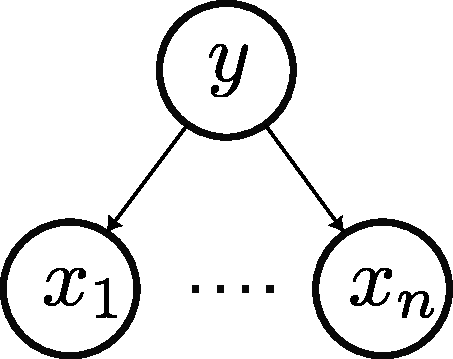
\includegraphics[scale=0.5]{./images/conditional_independence.pdf}
		\end{figure}
    \item This allows us to write the class conditional density as a product of one dimensional densities:
    $$p(\mathbf{x}|y=c, \boldsymbol{\theta}) = \prod_{j=1}^{D}p(x_j|y=c,\boldsymbol{\theta}_{jc})$$
  \end{itemize}
  The resulting model is called a \textbf{naive Bayes classifier (NBC)}. The model is called ``naive'' since we assume the independence between the features, which is not true in practice. However, if often results in classifiers that work well.

  The form of the class-conditional density depends on the type of each feature. We give some possibilities below:
  \begin{itemize}
    \item In the case of real-valued features, we can use the Gaussian distribution: $p(\mathbf{x}|y=c, \boldsymbol{\theta}) = \prod_{j=1}^{D}\mathcal{N}(x_j|\mu_{jc}^2)$, where $\mu_{jc}$ is the mean of feature $j$ in objects of class $c$, and $\sigma_{jc}^2$ is its variance.
    \item In the case of binary features, we can use the Bernoulli distribution: $p(\mathbf{x}|y=c, \boldsymbol{\theta}) = \prod_{j=1}^{D}\textrm{Ber}(x_j|\mu_{jc})$, where $\mu_{jc}$ is the probability that feature $j$ occurs in class $c$. This is sometimes called the \textbf{multivariate Bernoulli naive Bayes} model.
    \item In the case of categorical features, $x_j\in \{1,...,K\}$, we can model the multinomial distribution: $p(\mathbf{x}|y=c, \boldsymbol{\theta}) = \prod_{j=1}^{D}\textrm{Cat}(x_j|\mu_{jc})$, where $\boldsymbol{\mu}_{jc}$ is a histogram over the $K$ possible values for $x_j$ in class $c$.
  \end{itemize}

The probability for a single data case is given by
$$p(\mathbf{x}_i,y_i|\boldsymbol{\theta}) = p(y_i|\boldsymbol{\pi})\prod_{j}p(x_{ij}|\boldsymbol{\theta}_j)=\prod_{c}\pi_{c}^{\mathds{I}(y_i=c)}\prod_{j}\prod_{c}p(x_{ij}|\boldsymbol{\theta}_{jc})^{\mathds{I}(y_i=c)},$$
where $\boldsymbol{\pi}$ is a vector of class probability. Hence the log-likelihood is given by
	$$\textrm{log}p(\mathcal{D}|\boldsymbol{\theta}) = \sum_{c=1}^{C}N_c\textrm{log}\pi_c+\sum_{j=1}^{D}\sum_{c=1}^{C}\sum_{i:y_i=c}\textrm{log}p(x_{ij}|\boldsymbol{\theta}_{jc})$$

	\begin{algorithm}[H]
		\SetAlgoLined
%		\KwResult{Write here the result }
		Initialize $N_c=0,N_{jc}=0$ \;
		\For{$i=1:N$}{
      $c=y_i$ //Class label of $i$-th example;

      $N_c:=N_c+1$;

  		\For{$j=1:D$}{
      \uIf{$x_{ij}=1$}{
        $N_{jc}:=N_{jc}+1$
        }
  		}
		}
  $\hat{\pi}=\frac{N_c}{N},\hat{\theta}_{jc}=\frac{N_{jc}}{N_c}$
	\caption{Fitting a naive Bayes classifier to binary features}
\end{algorithm}

\section{Logistic Regression}
\label{sec:logistic_regression}

Logistic regression corresponds to the following binary classification model:
$$p(y|\mathbf{x},\mathbf{w})=\textrm{Ber}(y|\sigma(\mathbf{w}^T\mathbf{x}))$$

Logistic regression modles a logit (log odds) through a linear model. For binary data, the goal is to model the probability $p$ that one of two outcomes occurs. The logit function is $\textrm{log}\frac{p}{1-p}$, which varies between $-\infty$ and $+\infty$ as $p$ varies between $0$ and $1$.
$$\textrm{log}\frac{p}{1-p} = w_0x_0 +  w_1x_1 + ... + w_nx_n$$
Note that the logistic regression model assumes that the log-odds (\textit{logit}) of an observation $y$ can be expressed as a linear function. In this context, the logit function is called the \textbf{\textit{link function}} because it ``links'' the probability to the linear function of the predictor variables.

% Simplest solution to model a dependant variable $y$ is a linear regression. However, $y$ should be in a range of $[0,1]$. So we need to introduce the logit function. 

% The linear regression can be generalized to the classification setting with two changes:
% \begin{itemize}
% 	\item Replacing the Gaussian distribution for $y$ with a Bernoulli distribution: $p(y|\mathbf{x},\mathbf{w})=Ber(y|\mu(\mathbf{x}))$
% 	\item Squashing input data into sigmoid function $\sigma(\eta)$ that range from 0 to 1: $\sigma(\eta)\triangleq \frac{1}{1+exp(-\eta)}$.
% \end{itemize}
% $$p(y|\mathbf{x},\mathbf{w})=Ber(y|\sigma(\mathbf{w}^T\mathbf{x})),\$$

The negative log-likelihood for logistic regression is given by
\begin{align*}
	\textrm{NLL}(\mathbf{w}) &= -\sum_{i=1}^{N}\textrm{log}[\mu_i^{\mathds{I}(y_i=1)}\times (1-\mu_i)^{\mathds{I}(y_i=0)}]\\
	&=-\sum_{i=1}^{N}[y_i\textrm{log}\mu_i + (1-y_i) \textrm{log}(1-\mu_i)], \textrm{ }\footnotemark
\end{align*}
where $\mu=\sigma(\mathbf{w}^T\mathbf{x})$. This is also called \textbf{cross-entropy} error function. 
\footnotetext{$\mathds{I}(y_i=1) = y_i$, because $y_i\in \{0, 1\}$ is a binary variable}

Another way to express \textrm{NLL} is as follows. Suppose $\hat{y}_i\in\{-1,+1\}$ instead of $y_i\in\{0,1\}$. We have $p(y=1)=\frac{1}{1+\mathrm{exp}(-\mathbf{w}^T\mathbf{x})}$ and $p(y=-1)=\frac{1}{1+\mathrm{exp}(+\mathbf{w}^T\mathbf{x})}$. Hence
\begin{align*}
	\textrm{NLL}(\mathbf{w}) &= -\frac{1}{N}\sum_{n=1}^N [\mathbb{I}(\hat{y}_n=1)\log(\sigma(a_n))+\mathbb{I}(\hat{y}_n=-1)\log(\sigma(-a_n))]\\
							 &= -\frac{1}{N}\sum_{n=1}^N \log(\sigma(\hat{y}_na_n))\\
							 &=  \frac{1}{N}\sum_{i=1}^{N}\textrm{log}(1+\mathrm{exp}(-\hat{y}_i\mathbf{w}^T\mathbf{x}_i).
\end{align*}
Note that the sigmoid is used for compressing the output into $[0,1]$ and $\sigma(-a_n) = 1-\sigma(a_n)$. Unlike the linear regression, there is no closed from solution for logistic regression, thus we need optimization algorithms for it. Typically, optimization process involves the gradient and Hessian. 
\begin{align*}
	\mathbf{g}&=\frac{d}{d\mathbf{w}}\mathrm{NLL}(\mathbf{w})=\frac{d}{d\mu_i}\mathrm{NLL}(\mathbf{w})\frac{d\mu_i}{d\mathbf{h}}\frac{d\mathbf{h}}{d\mathbf{w}}\\
	& = \sum_{i=1}\Bigg[-\frac{y_i}{\mu_i} + \frac{(1-y_i) }{(1-\mu_i)}\Bigg]\frac{d\mu_i}{d\mathbf{h}}\frac{d\mathbf{h}}{d\mathbf{w}}=\sum_{i=1}\Bigg[\frac{\mu_i-y_i }{\mu_i(1-\mu_i)}\Bigg]\frac{d\mu_i}{d\mathbf{h}}\frac{d\mathbf{h}}{d\mathbf{w}}\\
	&=\sum_{i}(\mu_i-y_i)\mathbf{x}_i=\mathbf{X}^T(\boldsymbol{\mu}-\mathbf{y})\\
	\frac{d\mu_i}{d\mathbf{h}}& = \mu_i(1-\mu_i)\\
	\frac{d\mathbf{h}}{d\mathbf{w}}& = \mathbf{x}_i
\end{align*}
where $\mathbf{h}=\mathbf{w}^T\mathbf{x}$. 

We can also use the second-order method. 
\begin{align*}
\mathbf{H}&=\frac{d}{d\mathbf{w}}g(\mathbf{w})^T=\sum_{i}(\nabla_{\mathbf{w}}\mu_i)\mathbf{x}_i^T=\sum_{i}\mu_i(1-\mu_i)\mathbf{x}_i\mathbf{x}_i^T\\
&=\mathbf{X}^T\mathbf{S}\mathbf{X},
\end{align*}
where $\mathbf{S}\triangleq \mathrm{diag}(\mu_i(1-\mu_i))$. Note that $\mathbf{H}$ is positive definite, because the \textrm{NLL} is convex and has a global minimum. 

\section{Decision Tree}
In decision analysis, a decision tree can be used to visually and explicitly represent decisions and decision making. In data mining, a decision tree describes data (but the resulting classification tree can be an input for decision making).
\begin{itemize}
    \item Classification trees: Tree models where the target variable take a discrete set of values; in these tree structures, leaves represent class labels and branches represent conjunctions of features that lead to those class labels. 
    \item Regression trees: Decision trees where the target variable can take continuous values (typically real numbers). 
\end{itemize}
The term Classification And Regression Tree (CART) analysis is an umbrella term used to refer to both them.

Some techniques, often called ensemble methods, construct more than one decision tree:
\begin{itemize}
    \item Boosted tree: Incrementally building an ensemble by training each new instance to emphasize the training instances previously mis-modeled. A typical example is AdaBoost.
    \item Bootstrap aggregated (or bagged): decision trees, an early ensemble method, builds multiple decision trees by repeatedly resampling training data with replacement, and voting the trees for a consensus prediction, e.g., random forest.
    \item Rotation forest: in which every decision tree is trained by first applying principal component analysis (PCA) on a random subset of the input features
\end{itemize}

The basic algorithm used in decision trees is known as the ID3 (by Quinlan) algorithm. The ID3 algorithm builds decision trees using a top-down, greedy approach. Briefly, the steps to the algorithm are: Select the best attribute $\rightarrow$ Assign A as the decision attribute (test case) for the NODE. - For each value of A, create a new descendant of the NODE. - Sort the training examples to the appropriate descendant node leaf. - If examples are perfectly.

Now, the next big question is how to choose the best attribute. For ID3, we think of the best attribute in terms of which attribute has the most information gain, a measure that expresses how well an attribute splits that data into groups based on classification.

Pseudocode: ID3 is a greedy algorithm that grows the tree top-down, at each node selecting the attribute that best classifies the local training examples. This process continues until the tree perfectly classifies the training examples or until all attributes have been used.

The pseudocode assumes that the attributes are discrete and that the classification is binary. Examples are the training example. Target attribute is the attribute whose value is to be predicted by the tree. Attributes is a list of other attributes that may be tested by the learned decision tree. Finally, it returns a decision tree that correctly classifies the given Examples.

\subsection{Information Gain}
Information gain is a statistical property that measures how well a given attribute separates the training examples according to their target classification. As you can see in the Fig. \ref{fig:info_gain}, attribute with low information gain (right) splits the data relatively evenly and as a result doesn't bring us any closer to a decision. Whereas, an attribute with high information gain (left) splits the data into groups with an uneven number of positives and negatives and as a result helps in separating the two from each other.

\begin{figure}[h]
    \centering
    \begin{subfigure}{.4\textwidth}
        \centering
        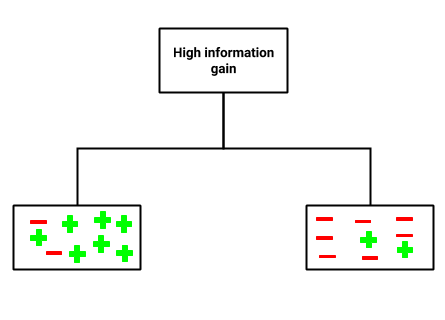
\includegraphics[scale=.45]{./images/decision_tree/high_gain.png}
        \caption{High information gain.}
        \label{fig:high_gain}
    \end{subfigure}
    \begin{subfigure}{.4\textwidth}
        \centering
        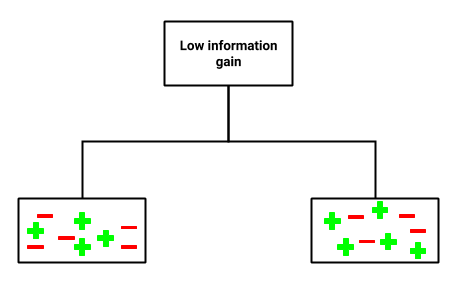
\includegraphics[scale=.45]{./images/decision_tree/low_gain.png}
        \caption{Low information gain.}
        \label{fig:low_gain}
    \end{subfigure}
    \caption{Information gain comparison.}
    \label{fig:info_gain}
\end{figure}

To define information gain precisely, we need to define a measure commonly used in information theory called entropy that measures the level of impurity in a group of examples. Mathematically, it is defined as:
$$Entropy = -\sum_i p_i \log p_i$$
, where $i$ is the class index. Since, the basic version of the ID3 algorithm deal with the case where classification are either positive or negative, we can define entropy as:
$$Entropy(S) = -p_+\log_2 p_+ - p_-\log_2 p_-$$
, where 
\begin{itemize}
    \item $S$: training examples
    \item $p_+$: is the proportion of positive examples in $S$
    \item $p_-$: is the proportion of negative examples in $S$
\end{itemize}

To illustrate, suppose $S$ is a sample containing 14 boolean examples, with 9 positive and 5 negative examples. Then, the entropy of $S$ relative to this boolean classification is:
$$Entropy([9+, 5-]) = -(9/14)\cdot \log_2(9/14) - (5/14)\cdot \log_2(5/14) = 0.940$$
Note that entropy is 0 if all the members of $S$ belong to the same class. For example, if all members are positive ($p_+$=1), then $p_-=0$, and $Entropy(S) = -1\cdot \log_2(1) -0\cdot \log_2(0) = 0$. Entropy is 1 when the sample contains an equal number of positive and negative examples. If the sample contains unequal number of positive and negative examples, entropy is between 0 and 1. The following figure shows the form of the entropy function relative to a boolean classification as $p_+$ varies between 0 and 1.

\begin{figure}[h]
    \centering
    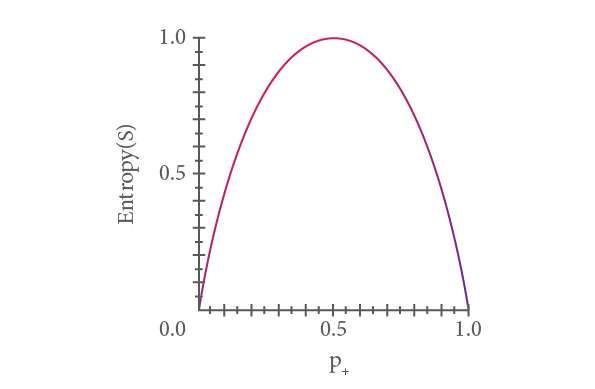
\includegraphics[scale=.40]{./images/decision_tree/entropy.jpg}
    \caption{Entropy.}
    \label{fig:entropy}
\end{figure}

Now, given entropy as a measure of the impurity in a sample of training examples, we can now define information gain as a measure of the effectiveness of an attribute in classifying the training data. Information gain, $Gain (S, A)$ of an attribute $A$, relative to a sample of examples $S$, is defined as:
$$Gain(S, A) \equiv Entrpoy(S) - \sum_{v \in Values(A)} \frac{|S_v|}{|S|} \cdot Entropy(S_v)$$
, where $|S_v|$ is a sample belongs to class $v$ and $|S|$ is the number of training samples. In other words,
$$\textrm{Gain  = Parent node of Entropy - [Average of Children Nodes Entropy]}$$




\section{Principal Component Analysis}
\subsection{Covariance and the weight vector}

When deriving PCA, we seek a vector \( \mathbf{w} \) (the weight vector or loading vector) such that the projection of the data onto this vector maximizes the variance. Maximizing the variance is equivalent to projecting the data onto a lower-dimensional linear subspace in such a way that the distance between a vector and its projection is not too large. For a given data matrix \( \mathbf{X} \) with mean zero (mean-centered data), the projection of the data onto \( \mathbf{w} \) is given by \( \mathbf{X}\mathbf{w} \).

The variance of the projected data can be expressed as:

\[
\text{Var}(\mathbf{X}\mathbf{w}) = \frac{1}{n} (\mathbf{X}\mathbf{w})^T (\mathbf{X}\mathbf{w}) = \frac{1}{n} \mathbf{w}^T \mathbf{X}^T \mathbf{X} \mathbf{w}
\]

Where \( n \) is the number of data points. The matrix \( \mathbf{X}^T \mathbf{X} \) is the covariance matrix of the data (up to a scaling factor).

The goal is to maximize the variance \( \mathbf{w}^T \mathbf{X}^T \mathbf{X} \mathbf{w} \) with respect to the weight vector \( \mathbf{w} \), subject to the constraint that \( \mathbf{w}^T \mathbf{w} = 1 \) (to prevent the trivial solution where the variance could be made arbitrarily large just by scaling \( \mathbf{w} \)).
\begin{align*}
	\mathcal{L} = \frac{1}{n} \mathbf{w}^\mathsf{T} \mathbf{X}^\mathsf{T} \mathbf{X} \mathbf{w} - \lambda \left( \mathbf{w}^\mathsf{T} \mathbf{w}  - 1 \right)
\end{align*}

\begin{align*}
	\frac{\partial \mathcal{L}}{\partial \mathbf{w}} = \frac{2}{n} \mathbf{X}^\mathsf{T} \mathbf{X} \mathbf{w} - 2 \lambda \mathbf{w} = \mathbf{0}
\end{align*}

\begin{align*}
	\underbrace{ \frac{1}{n} \mathbf{X}^\mathsf{T} \mathbf{X} }_{:= \mathbf{S} } \mathbf{w} = \lambda \mathbf{w}  \quad \Rightarrow \quad \mathbf{S} \mathbf{w} = \lambda \mathbf{w}
\end{align*}
This is exactly the eigenvalue equation. The eigenvectors $\rvw$ are the directions that maximize the variance, and the eigenvalues $\lambda$ represent the magnitude of the variance along those directions.

\begin{itemize}
	\item Eigenvectors: Each eigenvector of the covariance matrix represents a direction in the feature space. These directions are the principal components.
	\item Eigenvalues: The corresponding eigenvalue tells us how much variance is captured along that direction. The larger the eigenvalue, the more variance is captured by the corresponding eigenvector.
\end{itemize}

\[
\text{Var}(\mathbf{X}\mathbf{w}) = \frac{1}{n} (\mathbf{X}\mathbf{w})^T (\mathbf{X}\mathbf{w}) = \frac{1}{n} \mathbf{w}^T \mathbf{X}^T \mathbf{X} \mathbf{w} = \frac{1}{n} \mathbf{w}^T \mathbf{S} \mathbf{w} = \frac{1}{n} \mathbf{w}^T \lambda \mathbf{w} = \frac{1}{n} \lambda
\]

Capturing the Most Information:

\begin{itemize}
	\item Variance is a measure of how spread out the data is along a particular direction. By maximizing the variance, we ensure that the principal components capture the most significant patterns in the data.
	\item If we reduce the dimensionality by selecting components with the highest variance, we retain the most information about the data, effectively compressing the data without losing critical details.
	\item High variance indicates that the data points are spread out and less likely to be redundant. Conversely, low variance implies that data points are clustered close together, often making the information less significant.
\end{itemize}




\section{Latent Semantic Allocation}
\label{sec:lsa}

Topic model provides insights like
\begin{itemize}
	\item Can analyze topics. \eg, a certain topic includes specific words more than other topics. 
	\item A certain document's topic distribution (simplex)
\end{itemize}


pLSA: Latent Variable Model
$$P_{LSA}(w|d) = \sum_{z}P(w|z;\theta)P(z|d;\pi)$$
\begin{itemize}
	\item $w$: word
	\item $d$: document
	\item $z$: latent variable
\end{itemize}

Equivalently, 
$$P_{LSA}(d,w) = \sum_{z}P(w|z)P(d|z)p(z) = p(d)\sum_{z}P(w|z)P(z|d)$$

The probability of observing $n(w_i, d_j)$ occurrences of word $w_i$ in document $d_j$ is given by
$$p(w_i, d_j)^{n(w_i, d_j)}$$

The probability of observing the complete document collection is then given by the product of probabilities of observing every single word in every document with corresponding number of occurrences.

Then, the likelihood function becomes

$$L = \prod_{i=1}^{m}\prod_{j=1}^{n}p(w_i, d_j)^n(w_i, d_j)$$

The log-likelihood is then
\begin{align*}
	\mathcal{L} &= \sum_{i=1}^{m}\sum_{j=1}^{n}n(w_i, d_j)\log (p(w_i, d_j))\\
				&= \sum_{l=1}^kp(w_i|z_l)p(d_j|z_l)p(z_l) 
\end{align*}

Parameter Inference:
\begin{itemize}
	\item We cannot maximize the likelihood analytically because of the logarithm of the sum
	\item A standard procedure is to use \textit{EM}. 
\end{itemize}




\section{Latent Dirichlet Allocation}
\label{sec:topic_modeling_lda}

The assumptions of LDA:
\begin{itemize}
	\item Each topic is a distribution over words.
	\item Each document is a mixture of corpus-wide topics.
	\item Each word is sampled from one of topics. 
\end{itemize}
The LDA attempts to model the document generation process stochastically. However, we have to infer the latent structure (the distributions) of documents. 


\begin{figure}[h]
	\centering
	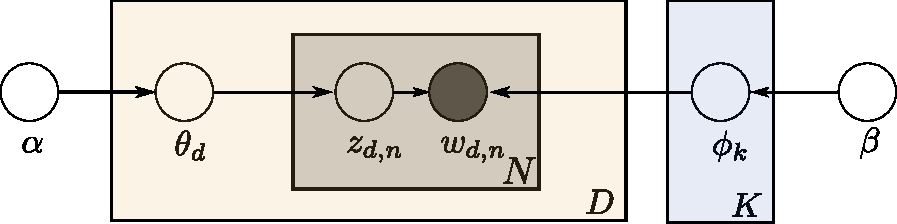
\includegraphics[scale=1.0]{./images/lda/lda.pdf}
\end{figure}
\begin{itemize}
	\item $\theta_d\sim Dir(\alpha)$: For each document, draw topic distribution. 
		\begin{itemize}
			\item $\alpha$: Dirichlet parameter
		\end{itemize}
	\item $z_{d,n}\sim Mult(\theta_d)$: per-word topic assignment. The $n$-th word of document $d$ is from which topic?
	\item $w_{d,n}\sim Mult(\phi_{z_{d,n}},n)$: observed word. The $n$-th word in a document $d$ is from a certain topic ($z_{d,n}$) distribution $\phi_{z_{d,n}}$.
	\item $\phi_k\sim Dir(\beta), i=\{1,\dots,K\}$: topics.
		\begin{itemize}
			\item $\beta$: topic hyperparameter (Dirichlet parameter).
		\end{itemize}
\end{itemize}
We can immediately notice that the LDA's modeling approach is quite far from the way we write texts. However, LDA works quite well. 

The document generation process can be modelled as follows:
\begin{align*}
	p(\phi_{1:K}, \theta_{1:D}, z_{1:D}, w_{1:D}) = \prod_{i=1}^K p(\phi_i|\beta)\prod_{d=1}^D p(\theta_d|\alpha)\Bigg(\prod_{n=1}^N p(w_{d,n}|\phi_{1:K},z_{d,n})p(z_{d,n}|\theta_d)\Bigg).
\end{align*}

\subsection{LDA Inference}
The posterior of the latent variables given the document is
\begin{align*}
	p(\phi, \theta, \mathbf{z}|\mathbf{w}) = \frac{p(\phi, \theta, \mathbf{z},\mathbf{w})}{\int_{\phi}\int_{\theta}\sum_{\mathbf{z}}p(\phi, \theta, \mathbf{z},\mathbf{w})}
\end{align*}
Computing the posterior is intractable:
\begin{itemize}
	\item The denominator is intractable
	\item We cannot compute the denominator, the marginal p(w).
	\item We are going to use collapsed Gibbs sampling. 
\end{itemize}

We want to estimate the topic distribution $\mathbf{z}$. 

\subsection{Dirichlet Distribution}
The Dirichlet Distribution can be considered as a extension of the \textit{beta distribution}. 
\begin{align}
	p(P=\{p_i\}|\alpha_i) = \frac{\Gamma(\sum_i\alpha_i)}{\prod_i\Gamma(\alpha_i)}\prod_ip_i^{\alpha_i-1}
	\label{eq:dirichlet_dist}
\end{align}
\begin{itemize}
	\item $\sum_ip_i = 1$
	\item The posterior distribution of Dirichlet distribution is also Dirichlet distribution. 
\end{itemize}

\chapter{Fourier Analysis}
Reference: Y.D. Chong 2021, NTU Lecture Note

The Fourier transform is one of the most important mathematical tools used for analyzing functions. Given an arbitrary function $f(x)$, with a real domain $(x \in \mathbb{R})$, we can express it as a linear combination of complex waves

\section{Fourier Series}
\label{sec:fourier_series}

We begin by discussing the Fourier series, which is used to analyze functions that are periodic in their inputs. A periodic function $f(x)$ is a function of a real variable $x$ that repeats itself every time $x$ changes by $a$. The constant $a$ is called the period. We can write the periodicity condition as
$$f(x+a) = f(x), \forall x\in \mathbb{R}.$$
The value of $f(x)$ can be real or complex, but $x$ should be real.

Let's consider what it means to specify a periodic function $f(x)$. One way to specify the function is to give an explicit mathematical formula for it. Another approach might be to specify the function values in $−a/2 \leq x < a/2$. Since there's an uncountably infinite number of points in this domain, we can generally only achieve an approximate specification of $f$ this way, by giving the values of $f$ at a large but finite set $x$ points. 

There is another interesting approach to specifying f. We can express it as a linear combination of simpler periodic functions, consisting of sines and cosines:
$$f(x) = \sum_{n=1}^{\infty} \alpha_n \sin\bigg(\frac{2\pi n x}{a}\bigg)+\sum_{m=0}^{\infty}\beta_m \cos\bigg(\frac{2\pi m x}{a}\bigg).$$
Note that the index $n$ does not include 0; since the sine term with $n = 0$ vanishes for all $x$, it's redundant. The above formula is called a \textit{Fourier series}. Given the numbers $\{\alpha_n, \beta_m\}$, which are called the \textit{Fourier coefficients}, $f(x)$ can be calculated for any $x$. The Fourier coefficients are real if $f(x)$ is a real function, or complex if $f(x)$ is complex.

\subsection{Square-integrable functions}
Can arbitrary periodic functions always be expressed as a Fourier series? It turns out that a certain class of periodic functions, commonly encountered in physical contexts, are guaranteed to always be expressible as Fourier series. These are called square-integrable functions such that the integral of the square of the absolute value is finite:
\begin{align*}
\int_{-a/2}^{a/2}|f(x)|^2 dx < \infty.
\end{align*}
Unless otherwise stated, we will always assume that the functions we're dealing with are square-integrable.

\subsection{Complex Fourier series and inverse relations}

We have written the Fourier series as a sum of sine and cosine functions. However, sines and cosines can be expressed by exponential functions by using \textit{Euler's formula}. 
\begin{align}
	e^{ix}=\cos x+i\sin x
	\label{eq:euler_formula}
\end{align}
\begin{itemize}
	\item $\cos x=\frac{e^{ix}+e^{-ix}}{2}$
	\item $\sin x=\frac{e^{ix}-e^{-ix}}{2i}$
\end{itemize}
Thus, Fourier series can be expressed as follows:
$$f(x) = \sum_{n=-\infty}^{\infty}e^{2\pi i n x/a}f_n$$
\begin{itemize}
	\item $i$: complex number
	\item $n$: integer
	\item $a$: period
	\item $f_n$: Fourier coefficient
\end{itemize}



\chapter{Training, Testing, and Regularization}
\section{Sources of Error in ML}
$$E_{out} \leq E_{ml}+\Omega$$
\begin{itemize}
	\item $E_{out}$: estimation of error. 
	\item $E_{ml}$: error from a learning algorithm
	\item $\Omega$: error caused by the variance from observations. 
\end{itemize}
We also define 
\begin{itemize}
	\item $f$: target function
	\item $g$: learning function
	\item $g^{(D)}$: learned function based on $D$, or simply \textit{hypothesis}.
	\item $D$: dataset drawn from the real world.
	\item $\bar{g}$: the average hypothesis of a given infinite number of $D$s. 
		$$\bar{g}(x) = \mathbb{E}_D[g^{(D)}(x)].$$
\end{itemize}

Error of a single instance $x$ from $g$ learnt from $D$ is given by
\begin{align*}
	Err_{\textrm{out}}(g^{(D)}(x)) = \mathbb{E}_{X}[(g^{(D)}(x)-f(x))^2],
\end{align*}
where $X$ can be considered as test sets. Then, the expected error over the infinite number of datasets $D$ sampled from a true data distribution is
\begin{align*}
	\mathbb{E}_D[Err_{\textrm{out}}(g^{(D)}(x))] &= \mathbb{E}_D[\mathbb{E}_{X}[(g^{(D)}(x)-f(x))^2]]\\
												 &= \mathbb{E}_X[\mathbb{E}_D[(g^{(D)}(x)-f(x))^2]]
\end{align*}
Let's simplify the term inside with an average of hypothesis $\bar{g}(x)$:
\begin{align*}
	\mathbb{E}_D[(g^{(D)}(x)-f(x))^2]&= \mathbb{E}_D[(g^{(D)}(x)-\bar{g}(x)+\bar{g}(x)-f(x))^2]\\
	&= \mathbb{E}_D\big[(g^{(D)}(x)-\bar{g}(x))^2+(\bar{g}(x)-f(x))^2\\ &\quad + 2 (g^{(D)}(x)-\bar{g}(x))(\bar{g}(x)-f(x))\big]\\
	&= \mathbb{E}_D\big[(g^{(D)}(x)-\bar{g}(x))^2\big]+(\bar{g}(x)-f(x))^2\\ &\quad + \mathbb{E}_D\big[2 (g^{(D)}(x)-\bar{g}(x))(\bar{g}(x)-f(x))\big]
\end{align*}
Since, $\mathbb{E}_D\big[2 (g^{(D)}(x)-\bar{g}(x))(\bar{g}(x)-f(x))\big]$ is 0, the expectation of the error becomes
\begin{align*}
	\mathbb{E}_D[Err_{\textrm{out}}(g^{(D)}(x))] = \mathbb{E}_X\big[\mathbb{E}_D\big[(g^{(D)}(x)-\bar{g}(x))^2\big]+(\bar{g}(x)-f(x))^2\big].
\end{align*}
Let's closely look at this formula. The errors are from two sources:
\begin{itemize}
	\item \textbf{Variance}: $\mathbb{E}_D\big[(g^{(D)}(x)-\bar{g}(x))^2\big]$. Variance captures how much your classifier changes if you train on a different training set. We need to collect more data to reduce the variance. 
	\item \textbf{Bias}: $(\bar{g}(x)-f(x))^2$. Bias is the inherent error that you obtain from your classifier even with infinite training data. We need to build a more complex model to reduce the bias. 
\end{itemize}
However, if we reduce the bias, then the variance tends to increase. 

\subsection{Alternative Derivation}

The derivation of the bias–variance decomposition for squared error proceeds as follows.[6][7] For notational convenience, abbreviate $f = f(x)$ and $\hat{f} = \hat{f}(x)$. First, recall that, by definition, for any random variable $\mathbf{X}$, we have
$$\displaystyle \operatorname {Var} {\big [}{\hat {f}}(x){\big ]}=\operatorname {E} [X^{2}]-\operatorname {E} [X]^{2}.$$
By rearranging, we get 
$$\operatorname {E} [X^{2}] = \displaystyle \operatorname {Var} {\big [}{\hat {f}}(x){\big ]}+\operatorname {E} [X]^{2}.$$
Since $f$ is deterministic
$$\operatorname {E} [f] = f$$

Thus, given $y = f+\varepsilon$ and $\operatorname {E} [\varepsilon] = 0$, implies $\operatorname {E} [y] = \operatorname {E} [f+\varepsilon] = \operatorname {E} [f] = f$

Also, since $\operatorname{Var} [\varepsilon ]=\sigma ^{2}$
$$\displaystyle \operatorname {Var} [y]=\operatorname {E} [(y-\operatorname {E} [y])^{2}]=\operatorname {E} [(y-f)^{2}]=\operatorname {E} [(f+\varepsilon -f)^{2}]=\operatorname {E} [\varepsilon ^{2}]=\operatorname {Var} [\varepsilon ]+{\Big (}\operatorname {E} [\varepsilon ]{\Big )}^{2}=\sigma ^{2}$$

Thus, since $\varepsilon$ and $\hat {f}$ are independent, we can write:
\begin{align*}
	\operatorname {E} {\big [}(y-{\hat {f}})^{2}{\big ]}&=\operatorname {E} {\big [}(f+\varepsilon -{\hat {f}})^{2}{\big ]}\\
	&=\operatorname {E} {\big [}(f+\varepsilon -{\hat {f}}+\operatorname {E} [{\hat {f}}]-\operatorname {E} [{\hat {f}}])^{2}{\big ]}\\
	&=\operatorname {E} {\big [}(f-\operatorname {E} [{\hat {f}}])^{2}{\big ]}+\operatorname {E} [\varepsilon ^{2}]+\operatorname {E} {\big [}(\operatorname {E} [{\hat {f}}]-{\hat {f}})^{2}{\big ]}+2\operatorname {E} {\big [}(f-\operatorname {E} [{\hat {f}}])\varepsilon {\big ]}+\\
	&\quad 2\operatorname {E} {\big [}\varepsilon (\operatorname {E} [{\hat {f}}]-{\hat {f}}){\big ]}+2\operatorname {E} {\big [}(\operatorname {E} [{\hat {f}}]-{\hat {f}})(f-\operatorname {E} [{\hat {f}}]){\big ]}\\
	&=(f-\operatorname {E} [{\hat {f}}])^{2}+\operatorname {E} [\varepsilon ^{2}]+\operatorname {E} {\big [}(\operatorname {E} [{\hat {f}}]-{\hat {f}})^{2}{\big ]}+\\
	&\quad 2(f-\operatorname {E} [{\hat {f}}])\operatorname {E} [\varepsilon ]+2\operatorname {E} [\varepsilon ]\operatorname {E} {\big [}\operatorname {E} [{\hat {f}}]-{\hat {f}}{\big ]}+2\operatorname {E} {\big [}\operatorname {E} [{\hat {f}}]-{\hat {f}}{\big ]}(f-\operatorname {E} [{\hat {f}}])\\
	&=(f-\operatorname {E} [{\hat {f}}])^{2}+\operatorname {E} [\varepsilon ^{2}]+\operatorname {E} {\big [}(\operatorname {E} [{\hat {f}}]-{\hat {f}})^{2}{\big ]}\\
	&=(f-\operatorname {E} [{\hat {f}}])^{2}+\operatorname {Var} [y]+\operatorname {Var} {\big [}{\hat {f}}{\big ]}\\
	&=\operatorname {Bias} [{\hat {f}}]^{2}+\operatorname {Var} [y]+\operatorname {Var} {\big [}{\hat {f}}{\big ]}\\
	&=\operatorname {Bias} [{\hat {f}}]^{2}+\sigma ^{2}+\operatorname {Var} {\big [}{\hat {f}}{\big ]}
\end{align*}

\chapter{Optimization}
\label{ch:optimization}

\section{Intuition of Gradient}

Gradient is a vector function that represents a direction of steepest increase of a function to be differentiated at a certain point. For example, a convex function $z = ax^2+by^2$ has a gradient $[2ax, 2by]$. Its steepest descent direction is $[-2ax, -2by]$. At the point $x_0,y_0$, the gradient direction for the function is $2ax_0(y-y_0) = 2by_0(x-x_0)$. But then the lowest point $(x,y) = (0,0)$ does not lie on the line. Thus, we cannot find that minimum point in one step of ``gradient descent''. The steepeset direction does not lead to the bottom of the bowl. 

\subsection{Gradient Descent Proof}

Most deep learning algorithms involve \textbf{optimization}.

\begin{itemize}
	\item The derivative of the objective function $f(\mathbf{x})$ provides the slope of $f(\mathbf{x})$ at the point $f(\mathbf{x})$.
	\item It tells us how to change $\mathbf{x}$ in order to make a small improvement in our goal.
\end{itemize}

	A function $f(\mathbf{x})$ can be approximated by its first-order Taylor expansion at $\bar{\mathbf{x}}$:
	$$f(\mathbf{x})\approx f(\bar{\mathbf{x}})+\nabla f(\bar{\mathbf{x}})^T(x-\bar{\mathbf{x}})$$
	Now let $\mathbf{d}\neq0, ||\mathbf{d}||=1$ be a direction, and in consideration of a new point $\mathbf{x}:=\bar{\mathbf{x}}+\mathbf{d}$, we define:
	$$f(\bar{\mathbf{x}}+\mathbf{d})\approx f(\bar{\mathbf{x}})+\nabla f(\bar{\mathbf{x}})^T\mathbf{d}$$

We would like to choose $\mathbf{d}$ that minimizes the function $f$. From the Cauchy-Schwarz inequality \footnote{Cauchy-Schwarz Inequaility: $|\mathbf{a}\cdot \mathbf{b}|\leq ||\mathbf{a}||\textrm{ } ||\mathbf{b}||$. Equality holds if and only if either $\mathbf{a}$ or $\mathbf{b}$ is a multiple of the other.}, we know that
$$\nabla f(\bar{\mathbf{x}})^T\mathbf{d}\leq ||\nabla f(\bar{\mathbf{x}})||\textrm{ }||\mathbf{d}||$$
with equality when $\mathbf{d}=\lambda \nabla f(\bar{\mathbf{x}})$, where $\lambda\in \mathbbm{R}$.

	Since we want to minimize the function $f$, we negate the steepest direction $\mathbf{d}^{*}$ so the iterations of steepest descent becomes
	$$\mathbf{x}^{(k+1)} = \mathbf{x}^{(k)} - \eta \nabla f(\mathbf{x}^{(k)})$$
	, where $k$ is the index of iteration step and $\eta$ is the learning rate parameter.



%	$\nabla f(\bar{\mathbf{x}})^T\mathbf{d}/||\mathbf{d}||\geq ||\nabla f(\bar{\mathbf{x}})||=\nabla f(\bar{\mathbf{x}})^T\Bigg(\frac{\nabla f(\bar{\mathbf{x}})}{||\nabla f(\bar{\mathbf{x}})||}\Bigg)$

\section{Normalized Gradient Descent}

The underlying issue of the vanila gradient descent is the presence of saddle points in nonconvex functions; the gradient $\nabla f(x)$ vanishes near saddle points, which causes GD to ``stall'' in neighboring regions. This both slows the overall convergence rate and makes detection of local minima difficult. The detrimental effects of this issue become particularly severe in high-dimensional problems where the number of saddle points may proliferate.


However, in the normalized gradient descent
$$ \frac{\nabla f(x)}{||\nabla f(x)||}$$
The normalized gradient preserves the direction of the gradient but ignores magnitude, because the normalization does not vanish near saddle points, the intuitive expectation is that NGD should not slow down in the neighborhood of saddle points and should therefore escape quickly. 

\section{Projected Gradient Descent}
Gradient Descent (GD) is a standard way to solve unconstrained optimization problem. Starting from an initial point $x\in \mathbbm{R}^n$, GD itereates until a stopping criterion is met. Projected Gradient Descent (PGD) is a way to solve constrained optimization problem. Consider a constraint set $\mathcal{Q}$, starting from a initial point $x_0 \in \mathcal{Q}$, PGD iterates the following equation until a stopping condition is met:
$$x_{k+1} = P_\mathcal{Q} \Big(x_k - t_k \nabla f(x_k)\Big),$$
where $P_\mathcal{Q}$ is the projection operator
$$P_\mathcal{Q}(x_0) = \argmin_{x\in \mathcal{Q}} \frac{1}{2}||x-x_0||^2_2$$
In other words, given a point $x_0$, $P_\mathcal{Q}$ tries to to find a point $x\in \mathcal{Q}$ which is ``closest''to $x_0$.


Note that a vector projection can be expressed as follows:
$$a_1 = ||\malthbf{a}||\cos \theta = \mathbf{a}\cdot \hat{\mathbf{b}} = \mathbf{a}\cdot \frac{\mathbf{b}}{||\mathbf{b}||}$$
Thus, a projection for unit $L_2$ ball is given by the solution of the equation as follows:
$$\mathbf{x} = \mathcal{P}_{||x||_2\leq 1}(\mathbf{y})$$
The solution is
$$\mathbf{x} = \frac{\mathbf{y}}{\max \{1,||\mathbf{y}||_2\}}$$
The ``geometric'' proof is given as follows: Let $\mathcal{S} = \{\mathbf{x}\in \mathbbm{R}^n: ||\mathbf{x}||_2 \leq 1\}.$
\begin{itemize}
		\item If $\mathbf{y}\in \mathcal{S}$, then $||y||_2\leq 1$ and $\mathbf{y}$ itself is the closest point to $\mathbf{y}$.
		\item If $\mathbf{y}\notin \mathcal{S}$, then $||y||_2> 1$ and the closest point $\mathbf{x}\in \mathcal{S}$ to $\mathbf{y}$ will be simply $\frac{\mathbf{y}}{||\mathbf{y}||_2}$ as the norm of $\frac{\mathbf{y}}{||\mathbf{y}||_2}=1$.
\end{itemize}
By combining the bost cases, we have
$$\mathbf{x} = \frac{\mathbf{y}}{\max \{1,||\mathbf{y}||_2\}}$$


\section{Exponentially Weighted Average}
\begin{align*}
    v_t = \beta v_{t-1} + (1-\beta) \theta_t
\end{align*}
Larger $\beta$ value covers more longer history. EMA is exponentially weighted average the previous result. 

\section{Bias Correction}
The initial values of $v_t$ will be very low which need to be compensated, since the curve starts from 0, there are not many values to average on in the initial points. Thus, the curve is lower than the correct value initially and then moves in line with expected values. The $\beta$ is the same as the averaging coefficient. As $t$ becomes large, the impact of the bias correction will be decreased. 
\begin{align*}
    v_t = \frac{v_t}{1-\beta^t}
\end{align*}


\section{Momentum}
Momentum can reduce the oscillation in the gradients. Let's say $w$ has a small value and $b$ is in charge of oscillation. Then momentum can cancel out $db$ by averaging them. 

\begin{align*}
    &v_{dw} = \beta v_{dw} + (1-\beta)dw \\
    &v_{db} = \beta v_{db} + (1-\beta)db \\
    & w = w-\alpha v_{dw}\\
    & b = b-\alpha v_{db}\\
\end{align*}

\section{Adagrad: Adaptive Gradient}
\begin{align*}
    &v_{dw} = v_{dw} + dw \cdot dw \\
	& w = w-\frac{\alpha}{\sqrt{v_{dw}}+\epsilon} v_{dw}\\
\end{align*}
A con of Adagrad is learning rate will become very small


\section{RMS Prop}

\begin{align*}
    &s_{dw} = \beta s_{dw} + (1-\beta)dw^2 \\
    &s_{db} = \beta s_{db} + (1-\beta)db^2 \\
	& w = w-\alpha  \frac{dw}{\sqrt{s_{dw}}}\\
	& b = b-\alpha \frac{db}{\sqrt{s_{db}}} \\
\end{align*}

\section{ADAM}
Its name is derived from adaptive moment estimation, and the reason it's called that is because Adam uses estimations of first and second moments of gradient to adapt the learning rate for each weight of the neural network. $N$-th moment of a random variable is defined as the expected value of that variable to the power of $n$. More formally:
$$m_n = \mathbbm{E}[X^n]$$

To estimates the moments, Adam utilizes exponentially moving averages, computed on the gradient evaluated on a current mini-batch:

Since $m$ and $v$ are estimates of first and second moments, we want to have the following property:
\begin{align}
	\mathbbm{E}[m_t] &= \mathbbm{E}[g_t]\\
	\mathbbm{E}[v_t] &= \mathbbm{E}[g_t^2]\\
\end{align}
Unbiased estimators

ADAM uses both momentum style and RMS prop style averaging. 
\begin{itemize}
	\item $v_{dw} = \beta v_{dw} + (1-\beta)dw$
	\item $v_{db} = \beta v_{db} + (1-\beta)db$
	\item $s_{dw} = \beta s_{dw} + (1-\beta)dw^2 $
	\item $s_{db} = \beta s_{db} + (1-\beta)db^2 $
\end{itemize}

Using them,
\begin{itemize}
	\item $ v^{\textrm{corr}}_{dw} = \frac{v_{dw}}{1-\beta_1^t}$
	\item $ v^{\textrm{corr}}_{db} = \frac{v_{db}}{1-\beta_1^t}$
	\item $ s^{\textrm{corr}}_{dw} = \frac{s_{dw}}{1-\beta_2^t}$
	\item $ s^{\textrm{corr}}_{db} = \frac{s_{db}}{1-\beta_2^t}$
\end{itemize}

Finally, 
\begin{align*}
	& w = w-\alpha  \frac{v^{\textrm{corr}}_{dw}}{\sqrt{s^{\textrm{corr}}_{dw}}+\varepsilon}\\
	& b = b-\alpha  \frac{v^{\textrm{corr}}_{db}}{\sqrt{s^{\textrm{corr}}_{db}}+\varepsilon}\\
\end{align*}





\part{Regression}
\chapter{Ensemble Learning}

\section{Bagging}

\textit{Bagging} (bootstrap aggregating) is a simple way to make a noisy model more stable. Imagine you have a wobbly predictor-like a deep decision tree-that can change its mind a lot if the training data changes a little. Instead of trusting a single tree, bagging builds many versions of that model on slightly different views of the data, and then averages their answers (or takes a majority vote for classification). Averaging smooths out the noise, so the final prediction is steadier and usually more accurate.


How do we get those slightly different views? That's where bootstrapping comes in. From the original training set, we repeatedly draw new datasets of the same size with replacement (so the same example can appear multiple times, and some examples are left out). Each bootstrapped dataset trains its own model. Because each model sees a different sample, their mistakes won't line up perfectly—averaging then cancels out a lot of the randomness.

Why does this help? Many models, especially high-variance ones like decision trees, can overfit the quirks of a single dataset. Bagging reduces variance by blending many perspectives, without increasing bias too much. In practice, this often yields a solid accuracy boost and better reliability. A nice side effect is you get out-of-bag estimates: the examples left out of each bootstrap can be used as a built-in validation set to measure performance without a separate hold-out.

Bagging isn't magic—if the base model is already very stable (low variance) or consistently biased in the wrong direction, averaging won't fix the core problem. It also costs more compute and can feel less interpretable since you're dealing with many models instead of one. But as a foundational ensemble idea, bagging is both elegant and powerful—and it's the backbone of methods like Random Forests, which add an extra twist by randomly selecting features, too.

\subsection{Intuition}


We start with a single training set ($D={(x_i,y_i)}_{i=1}^n$). Instead of hoping for many independent datasets, we \textbf{simulate} them by drawing \textbf{bootstrap samples} ($D_1,\dots,D_M$): each ($D_m$) is formed by sampling ($n$) examples \textbf{with replacement} from ($D$). For each ($D_m$), we fit a base learner ($h_m$) (\eg a decision tree, ridge regression, logistic regression). We then \textbf{aggregate} the models:
\begin{align*}
	\bar{h}(x)=\frac{1}{M}\sum_{m=1}^{M}h_m(x).
\end{align*}

If we could draw truly independent datasets ($D^{(1)},\dots,D^{(M)}$) from the population and train ($h^{D^{(m)}}$) on each, then the \textbf{empirical average hypothesis} would converge to the \textbf{theoretical average hypothesis} ($\mathbb{E}_D[h^D(x)]$) as ($M\to\infty$). With bagging, our bootstraps come from the \textbf{empirical distribution} of ($D$), not the population, so they're not independent. 

\begin{itemize}
	\item Each bootstrap sample is just a reshuffled, reweighted version of the same original points.
	\item So two bootstrap samples will overlap a lot (they reuse the same observations), unlike two brand-new datasets collected from the real world.
	\item In short: they're new mixes of the same ingredients, not new ingredients.
\end{itemize}

Still, two facts make bagging effective:
\begin{enumerate}
	\item \textbf{Variance reduction by averaging}: Training many models on these different mixes and averaging their predictions smooths out noise (reduces variance), especially for models that change a lot when the data changes (like deep trees).
	\item \textbf{Bootstrap as a population proxy}: Drawing with replacement from ($D$) mimics sampling from the underlying data-generating process via the empirical distribution. This is not perfect independence, but for many learners it's good enough to bring ($\bar h$) close to ($\mathbb{E}_D[h^D(x)]$) in practice, especially for unstable learners (small data perturbations $\to$ large model changes), like deep decision trees.
\end{enumerate}

\subsection{Bias–variance intuition}

\begin{itemize}
	\item Variance: Bagging typically decreases variance because averaging stabilizes predictions.
	\item Bias: Bagging usually does not increase bias, and may slightly reduce it for some learners. But its main win is variance.
	\item Who benefits most? Unstable learners (\eg trees, k-NN with small ($k$)) benefit a lot. Stable learners (\eg linear/ridge regression) benefit less, though averaging can still help in noisy regimes.
\end{itemize}

Their are some costs: 
\begin{itemize}
	\item Interpretability
	\item Computational costs
\end{itemize}

## When and why it works (and when it doesn't)

\begin{itemize}
	\item Correlation matters. If base learners are too correlated, variance reduction is limited. This is why Random Forests add feature subsampling at each split to further decorrelate trees, improving over plain bagging of trees.
	\item Computational cost. Training ($M$) models costs ($M\times$) as much compute (though it parallelizes nicely).
	\item Interpretability. An averaged ensemble is harder to interpret than a single model (especially vs. a small tree or linear model). You can mitigate with feature importance, partial dependence, SHAP, and so on., but it's still less transparent.
	\item Diminishing returns in ($M$). Gains flatten as (M) grows because you approach the correlation floor. In practice, tens to a few hundreds of models are often sufficient.
\end{itemize}

\section{Boosting}

Boosting builds a strong model by adding many small, simple models (weak learners) sequentially. Each new model focuses on the mistakes of the models before it. In the end, we add their predictions to get one strong predictor.

\begin{itemize}
	\item Bagging = parallel averaging to reduce \textbf{variance}.
	\item Boosting = sequential fixing to reduce \textbf{bias} (and often variance too).
\end{itemize}

Types of Boosting Algorithms:
\begin{itemize}
	\item AdaBoost (Adaptive Boosting)
	\item Gradient Tree Boosting
	\item XGBoost
\end{itemize}

\subsection{AdaBoost}

Boosting is a general strategy for learning classifiers by combining simpler ones. The idea of boosting is to take a ``weak classifier'' - that is, any classifier that will do at least slightly better than chance — and use it to build a much better classifier, thereby boosting the performance of the weak classification algorithm. This boosting is done by averaging the outputs of a collection of weak classifiers. 

The most popular boosting algorithm is \textit{AdaBoost}, so-called because it is ``adaptive.'' AdaBoost is extremely simple to use and implement (far simpler than SVMs), and often gives very effective results. There is tremendous flexibility in the choice of weak classifier as well. Boosting is a specific example of a general class of learning algorithms called ensemble methods, which attempt to build better learning algorithms by combining multiple simpler algorithms.

Suppose we are given training data $\{(\rvx_i, y_i)\}^N_{i=1}$, where $\rvx_i \in \mathbb{R}^K$ and $y_i \in \left\{-1, 1\right\}$. And suppose we are given a (potentially large) number of weak classifiers, denoted $f_m(\rvx) \in \left\{-1, 1\right\}$, and a \textbf{0-1} loss function $I$, defined as
\begin{align*}
	I(f_m(\rvx), y) = \begin{cases}
		0&\text{ if } f_m(\rvx_i)=y_i\\
		1&\text{ if } f_m(\rvx_i)\neq y_i
	\end{cases}
\end{align*}
\begin{itemize}
	\item $I=0$ if prediction equals the truth ( $\hat{y}=y$)
	\item $I=1$ if prediction is wrong ( $\hat{y}\neq y$)
\end{itemize}

AdaBoost aims to build a strong classifier by combining many weak ones. It does this in rounds $m=1,2,\dots,M$ :

\begin{enumerate}
	\item Start fair: Give every training example the same weight (everyone is equally important at the beginning).
	\item Fit a weak learner on the weighted data
	\item Compute how good it is: measure its weighted error of weak learner $f_m$, $e_m$. 
		\begin{align*}
			e_m = \sum_{i=1}^{N}w_i^m \cdot I(f_m(\rvx_i), y_i),
		\end{align*}
		where $w_i^m$ is the current example weight. 
	\item Give it a vote: compute $\alpha_m$ (bigger when $e_m$ is smaller). 
		\begin{align*}
			\alpha_m = \frac{1}{2}\ln \left(\frac{1-e_m}{e_m}\right).
		\end{align*}
	\item Focus on the hard cases
	\item Repeat: fit the next weak learner on the reweighted data, and so on.
\end{enumerate}

After learning, the final classifier is based on a linear combination of the weak classifiers:
\begin{align*}
	\sum_m \alpha_mf_m(\rvx).
\end{align*}






\part{Kernel Methods}
\chapter{Kernel Methods}
\begin{itemize}
	\item The main idea is to use large set of fixed non-linear basis functions.
	\item The complexity depends on number of basis functions, but dual trick changes it to a size of dataset. 
\end{itemize}

Kernel function: Let $\phi(\rvx)$ be a set of basis functions that map inputs $\rvx$ to a feature space. In many algorithms, this feature space only appears in a dot product $\phi(\rvx)^T\phi(\rvx')$ of input pairs $\rvx$ and $\rvx'$. Then, kernel function can be defined as $k(\rvx, \rvx') = \phi(\rvx)^T\phi(\rvx')$. Note that we only need to know $k(\rvx, \rvx')$, not $\phi(\rvx)$.
\begin{itemize}
	\item The kernel function is a measure of similarity between $\rvx_i$and $\rvx_j$ 
\end{itemize}

A function $k: \mathbb{R}^d\times \mathbb{R}^d\to \mathbb{R}$ is said to be a positive semidefinite kernel if it is symmetric, (\ie $k(\rvx',\rvx)= k(\rvx,\rvx')$).

Recall that the linear regression can be modelee as follows:
$$f(\rvx) = \rvx^T\rvw,$$
where $\rvx = [x_1, \dots, x_m]^T$ and $\rvw = [w_1,\dots,w_m]$. The ridge regression for $\mathbf{X}\in \mathbb{R}^{n\times m}$ matrix can be modeled as follows:
\begin{align}
	J(\rvw) &= \|\mathbf{y}-\mathbf{X}\rvw\|^2_2 + \lambda \|\rvw\|^2_2 \\
			&= (\mathbf{y}-\mathbf{X}\rvw)^T(\mathbf{y}-\mathbf{X}\rvw)+\lambda\rvw^T\rvw\\
			&= (\mathbf{y}^T-\rvw^T\mathbf{X}^T)(\mathbf{y}-\mathbf{X}\rvw)+\lambda\rvw^T\rvw\\
			&= \rvy^T\rvy-\rvw^T\mathbf{X}^T\rvy-\rvy^T\mathbf{X}\rvw+\rvw^T\mathbf{X}^T\mathbf{X}\rvw+\rvw^T\lambda\mathbf{I}\rvw\\
	\frac{\partial J}{\partial \rvw}&= -\mathbf{X}^T\rvy-\mathbf{X}^T\rvy+\mathbf{X}^T\mathbf{X}\rvw+\mathbf{X}^T\mathbf{X}\rvw+2\lambda\mathbf{I}\rvw = 0\\
	\rvw	&= (\mathbf{X}^T\mathbf{X}+\lambda\mathbf{I})^{-1}\mathbf{X}^T\rvy
	\label{eq:ridge_regression}
\end{align}
Let's change it into a dual form:
\begin{align}
	(\mathbf{X}^T\mathbf{X}+\lambda\mathbf{I})\rvw	&= (\mathbf{X}^T\mathbf{X}+\lambda\mathbf{I})(\mathbf{X}^T\mathbf{X}+\lambda\mathbf{I})^{-1}\mathbf{X}^T\rvy\\
	(\mathbf{X}^T\mathbf{X}+\lambda\mathbf{I})\rvw &= \mathbf{X}^T\rvy\\ 
	\rvw &= \lambda^{-1}\mathbf{I}(\mathbf{X}^T\rvy-\mathbf{X}^T\mathbf{X}\rvw)\\
	&= \mathbf{X}^T\lambda^{-1}(\rvy-\mathbf{X}\rvw)\\
	&= \mathbf{X}^T\alpha\\
	\lambda\alpha &= (\rvy-\mathbf{X}\rvw)\\
	&= (\rvy-\mathbf{X}\mathbf{X}^T\alpha)\\
	\rvy &= (\mathbf{X}\mathbf{X}^T\alpha+\lambda\alpha)\\
	\alpha &= (\mathbf{X}\mathbf{X}^T+\lambda)^{-1}\rvy\\
	\alpha &= (\mathbf{G}+\lambda)^{-1}\rvy,
	\label{eq:dual_regression}
\end{align}
where $\mathbf{G} = \mathbf{X}\mathbf{X}^T$ is a \textit{Gram matrix}. Thus, we just have to solve $m\times m$ matrix. 

Therefore, given a new input $\rvx'\in \mathbb{R}^m$, the prediction $f(\rvx') = (\rvx')^T\rvw $ can be expressed as follows:
$$f(\rvx') = (\rvx')^T\mathbf{X}^T(\mathbf{X}\mathbf{X}^T+\lambda\mathbf{I})^{-1}\rvy.$$

Note that this formula depends only on the data via inner products. 
\begin{align*}
	(\rvx')^T\mathbf{X}^T = 
	\begin{bmatrix}
		\langle \rvx',\rvx_1\rangle\\
		\vdots\\
		\langle \rvx',\rvx_n\rangle
	\end{bmatrix}^T,\quad
	\mathbf{X}\mathbf{X}^T = 
	\begin{bmatrix}
		\langle \rvx_1,\rvx_1\rangle& \dots& \langle \rvx_1,\rvx_n\rangle\\
		\vdots&\ddots&\vdots\\
		\langle \rvx_n,\rvx_1\rangle &\dots &\langle \rvx_n,\rvx_n\rangle
	\end{bmatrix}
\end{align*}
Therefore, we can apply the kernel trick and consider the more general prediction function.


% Then, the closed-form solution of the ridge regression is given by
% $$\hat{\boldsymbol{\theta}} = (\mathbf{X}^T\mathbf{X}+\lambda\mathbf{I})^{-1}\mathbf{X}^T\mathbf{y}.$$


% We can rewrite it by $\rvw = \Phi \rva$, where $\Phi = [\phi(\rvx_1),\dots,\phi(\rvx_N)]$, $\rva = [a_1,\dots,a_N]^T$, and $a_n =-\frac{1}{\lambda} (\rvw^T\phi(\rvx_n)-y_n).$. Then, we get a dual objective, which aims to minimize $E$ with respect to $\rva$.

% Let $K = \Phi^T\Phi$ be the Gram matrix. 


\section{Gaussian Process}
\label{sec:gaussian_process}
Gaussian processes are distributions over functions $f(x)$ of which the distribution is defined by a mean function $m(x)$ and positive definite covariance function $k(x,x')$:
$$f(x) \sim \mathcal{GP}(m(x),k(x,x')).$$

Let $f(x) = \phi(x)^Tw$, with $w\sim \mathcal{N}(0, \alpha^{-1}\mathbf{I})$. Then, $m(x) = \mathbb{E}[f(x)] = \mathbb{E}[w]^T\phi(x) = 0$

$k(x, x') = \mathbb{E}[(f(x)-m(x))(f(x')-m(x'))] =\mathbb{E}[f(x)(f(x')] $


\chapter{Support Vector Machine}
\section{Introduction}

\subsection{Orthogonal Projection}
Given two vectors $x$ and $y$, we would like to find the orthogonal projection of $x$ onto $y$.

By definition:
$$||z|| = ||x||cos(\theta).$$
Note that the dot product of $x$ and $y$ is 
$$cos(\theta)= \frac{x\cdot y}{||x||\cdot||y||}.$$
So we can replace the cosine 
$$||z|| = ||x||\frac{x\cdot y}{||x||\cdot||y||}.$$
This results in 
$$||z|| = u\cdot x,$$
where $u$ is an unit vector of $y$, which has the same direction as $z$. Therefore we can express $z$ as follows: 
$$z = ||z||\cdot u,$$
Then, 
\begin{align*}
	z &= (u\cdot x)u.
\end{align*}
Equivalently, 
\begin{align*}
	\textrm{Proj}_yx &= \Bigg(\frac{y\cdot x}{||y||^2}\Bigg)y.
\end{align*}

\section{Decision Boundary with Margin}

Support vectors are the data points that lie closest to the decision surface(or hyperplane). They are directly related to the optimal hyperplane. The goal of SVM is to find the optimal separating hyperplane which maximizes the margin of the training data. The hyperplane can be written as the set of points $\mathbf{x}$, satisfying 
$$\mathbf{w}\cdot \mathbf{x}+b=0$$
Note that the hyperplain is normal to the vector $\mathbf{w}$. 
$$\mathbf{w}(\mathbf{x}-\mathbf{x}_0)=0,$$
where $b = \mathbf{w}\cdot\mathbf{x}_0$. However, what is the optimal separating hyperplanes? The optimal hyperplane is the one which maximizes the margin of the training data. SVMs maximize the margin around the separating hyperplane. The decision function is fully specified by a subset of training samples, the support vectors. Let's consider a simple case, where training data is linearly separable, $\mathcal{D} = \left\{ (\mathbf{x}_i, y_i)\mid\mathbf{x}_i \in \mathbb{R}^p,\, y_i \in \{-1,1\}\right\}_{i=1}^n$. Then, we can build two hyperplanes separating the data with no points between them:
\begin{itemize}
	\item $H_1:\mathbf{w}\cdot \mathbf{x}+b=1$
	\item $H_2:\mathbf{w}\cdot \mathbf{x}+b=-1$
\end{itemize}

There are two constraints:
\begin{enumerate}
	\item $\mathbf{w}\cdot \mathbf{x}+b\geq1$
	\item $\mathbf{w}\cdot \mathbf{x}+b\leq-1$
\end{enumerate}
These can be combined as follows:
$$y(\mathbf{w}\cdot \mathbf{x}+b)\geq 1.$$

To maximize the margin, we can consider a unit vector $\mathbf{u} = \frac{\mathbf{w}}{||\mathbf{w}||}$, which is perpendicular to the hyperplanes and a point $x_0$ on the hyperplane $H_2$. If we scale $u$ from $x_0$, we get $z = x_0+ru$. If we assume $z$ is on $H_1$, then $\mathbf{w}\cdot z +b=1$. This is equivalent to 
\begin{align*}
	\mathbf{w}\cdot (x_0+ru)+b=1\\
	\mathbf{w}x_0+\mathbf{w}r\frac{\mathbf{w}}{||\mathbf{w}||}+b=1\\
	\mathbf{w}x_0+r||\mathbf{w}||+b=1\\
	\mathbf{w}x_0+b=1-r||\mathbf{w}||
\end{align*}
$x_0$ is on $H_2$, so $\mathbf{w}x_0+b=-1$
\begin{align*}
	-1=1-r||\mathbf{w}||\\
	r=\frac{2}{||\mathbf{w}||}
\end{align*}
Note that the scaled unit vector $ru$'s magnitude is $r$. Thus, the maximization of margin is equivalent to maximize $r$. To maximize $r$, it is important to minimize the norm of $\mathbf{w}$. This is equivalent to an optimization problem. 
\begin{align*}
	&\min ||w||,\quad \textrm{subject to } \\
	&y_i(\mathbf{w}\cdot \mathbf{x}_i+b)\geq 1 \quad\forall i.
\end{align*}
This minimization problem gives the same result as the following:  
\begin{align*}
	&\min \frac{1}{2}||w||^2,\quad \textrm{subject to } \\
	&y_i(\mathbf{w}\cdot \mathbf{x}_i+b)\geq 1 \quad\forall i.
\end{align*}
Now, we now have \textbf{convex quadratic optimization problem}. However, this hard margin cannot tolerate erroneous cases. There could be two solutions:
\begin{itemize}
	\item Admits prediction errors. 
	\item Use non-linearity (complex decision boundary).
\end{itemize}

\section{Error Handling in SVM}
Let's first try to solve the issue by allowing some prediction errors. 
\begin{align*}
	&\min ||w||+C\cdot N_{e},\quad \textrm{subject to } \\
	&y_i(\mathbf{w}\cdot \mathbf{x}_i+b)\geq 1 \quad \forall i.
\end{align*}
where $N_e$ is the number of errors. It means we consider all errors equally. This penalty approach is \textbf{0-1 loss}. This approach is not popular, since it is hard to solve. Another approach is to use a \textbf{slack variable} with \textbf{hinge loss}, instead of counting the number of errors. 
\begin{align*}
	&\min ||w||+C\sum_j\xi_j ,\quad \textrm{subject to } \\
	&y_i(\mathbf{w}\cdot \mathbf{x}_i+b)\geq 1-\xi_j \quad \forall i,\, \xi_j\geq 0,\, \forall j.
\end{align*}
Note that $\xi_j>1$ when mis-classified by its definition: 
\begin{align*}
	\xi_j = (1-(\mathbf{w}x_j+b)y_j)_+
\end{align*}
Let's look at the new constraint. If some data points are mis-classified, then $\xi_j>1$ and $y_i(\mathbf{w}\cdot \mathbf{x}_i+b)\leq 0$. This approach is called \textbf{soft-margin SVM}. Lastly, how do we set $C$?

\section{Kernel Trick}
\label{sec:kernel_trick}
Applying the kernel trick simply means replacing the dot product of two examples in a dual form by a kernel function. 

\begin{align}
	 \max_\alpha \sum_i \alpha_i -\frac{1}{2}\sum_i\sum_j \alpha_i\alpha_j y_iy_j \psi(\mathbf{x}_i)\cdot \psi(\mathbf{x}_j)
	 \label{eq:kernel_dual_form}
\end{align}
Equivalently, 
\begin{align}
	 \max_\alpha \sum_i \alpha_i -\frac{1}{2}\sum_i\sum_j \alpha_i\alpha_j y_iy_j K(\mathbf{x}_i,\mathbf{x}_j)
\end{align}














\section{SVM Optimization: Lagrange Multipliers}

\begin{align*}
&\min_{\rvx} f(\rvx) \\
&\textrm{subject to}\quad g(\rvx)=0.\\
\end{align*}
The minimum of $f$ is found when its gradient point in the same direction as the gradient of $g$. In other words, when:  
$$\nabla f(\rvx) = \alpha\nabla g(\rvx)$$
So if we want to find the minimum of $f$ under the constraint $g$, we just need to solve the following function: 
$$\mathcal{L}(\rvx, \alpha) = f(\rvx) - \alpha g(\rvx)$$
Note that the $\alpha$ is called a \textit{Lagrange multiplier}. 

Recall that we want to solve the following convex quadratic optimization problem:
\begin{align*}
	&\min \frac{1}{2}||w||^2,\quad \textrm{subject to } \\
	&y_i(\mathbf{w}\cdot \mathbf{x}_i+b)\geq 1 \quad\forall i.
\end{align*}
We can reformulate the above problem as follows:
\begin{align}
	\mathcal{L}(\rvw, b, \alpha) = \frac{1}{2}||w||^2 - \sum_i \alpha_i \Big[y_i(\mathbf{w}\cdot \mathbf{x}_i+b)-1\Big]
	\label{eq:objective_function}
\end{align}
We could try to solve the optimization problem, but this problem can only be solved analytically when the number of examples is small. Thus, we will reformulate the problem in the duality principle. 

To get the solution of the primal problem, we need to solve the following \textbf{Lagrangian problem}: 
\begin{align*}
	&\max_{\mathbf{w}, b}\min_\alpha \mathcal{L}(\rvw, b, \alpha)\\
	&\textrm{subject to}\quad \alpha_i\geq 0, \forall i.\\
\end{align*}

You may have noticed that the method of Lagrange multipliers is used for solving problems with equality constraints, and here we are using them with inequality constraints. This is because the method still works for inequality constraints, provided some additional conditions (the \textbf{KKT conditions}) are met. We will discuss about this soon.

\section{The Wolfe Dual Problem}
The Lagrangian problem has $m$ inequality constraints (where $m$ is the number of training examples) and is typically solved using its \textit{dual form}. The duality principle tells us that \textbf{an optimization problem can be viewed from two perspectives}: \Ni The first one is the \textit{primal problem}, a minimization problem in our case. \Nii The other one is the \textit{dual problem}, which will be a maximization problem. What is interesting is that the maximum of the dual problem will always be less than or equal to the minimum of the primal problem (we say it \textbf{provides a lower bound to the solution of the primal problem}). 

In our case, we are trying to solve a convex optimization problem, and \textbf{Slater's condition} holds for affine constraints (Gretton, 2016), so Slater’s theorem tells us that strong duality holds. Note that the strong duality denotes that the solutions from the dual and the primal are identical (the maximum of the dual problem is equal to the minimum of the primal problem). 

Solving the minimization problem involves taking the partial derivatives of $\mathcal{L}$ with respect to $\rvw$ and $b$.  
\begin{align*}
	&\nabla_\rvw\mathcal{L}(\rvw, b, \alpha) = \rvw - \sum_i \alpha_i y_i \mathbf{x}_i\\
	& \nabla_b\mathcal{L}(\rvw, b, \alpha) = -\sum_i \alpha_i y_i
\end{align*}
The first term gives
\begin{align*}
	&\rvw = \sum_{i=1}^m \alpha_i y_i \mathbf{x}_i\\
\end{align*}
Let's substitute the objective function \Cref{eq:objective_function} with $\rvw$:
\begin{align*}
	\mathbf{W}(\alpha, b) &= \frac{1}{2}\Big(\sum_i \alpha_i y_i \mathbf{x}_i\Big)\cdot \Big(\sum_j \alpha_j y_j \mathbf{x}_j\Big) - \sum_i \alpha_i \Bigg[y_i\Bigg(\Big(\sum_j \alpha_j y_j \mathbf{x}_j\Big)\cdot \mathbf{x}_i+b\Bigg)-1\Bigg]\\
						  &= \frac{1}{2}\Big(\sum_i\sum_j \alpha_i\alpha_j y_iy_j \mathbf{x}_i\cdot \mathbf{x}_j\Big) - \sum_i \alpha_i \Bigg[y_i\Bigg(\Big(\sum_j \alpha_j y_j \mathbf{x}_j\Big)\cdot \mathbf{x}_i+b\Bigg)\Bigg]+\sum_i \alpha_i \\
						  &= \frac{1}{2}\sum_i\sum_j \alpha_i\alpha_j y_iy_j \mathbf{x}_i\cdot \mathbf{x}_j - \sum_i\sum_j \alpha_i\alpha_j y_iy_j \mathbf{x}_i \cdot \mathbf{x}_j-\sum_i \alpha_i y_i b+\sum_i \alpha_i \\
						  &= \sum_i \alpha_i -\frac{1}{2}\sum_i\sum_j \alpha_i\alpha_j y_iy_j \mathbf{x}_i\cdot \mathbf{x}_j-\sum_i \alpha_i y_i b
\end{align*}
There is still $b$, but $b=0$, so we can just remove it. Finally, we get
\begin{align}
	 \mathbf{W}(\alpha, b) = \sum_i \alpha_i -\frac{1}{2}\sum_i\sum_j \alpha_i\alpha_j y_iy_j \mathbf{x}_i\cdot \mathbf{x}_j
	 \label{eq:dual_form}
\end{align}
This is the \textbf{Wolfe dual Lagrangian function}. Note that we transform the problem as a problem with regard to $\alpha$. Also, this is again a quadratic programming problem. The optimization problem is also called the \textbf{Wolfe dual problem}: 
\begin{align*}
	 &\max_\alpha \mathbf{W}(\alpha, b) = \sum_i \alpha_i -\frac{1}{2}\sum_i\sum_j \alpha_i\alpha_j y_iy_j \mathbf{x}_i\cdot \mathbf{x}_j\\
	 &\textrm{subject to } \alpha_i\geq 0 \textrm{ for any } i=1,\dots,m\\
	 & \sum_{i=1}^m \alpha_iy_i=0
\end{align*}
Once we get the value of $\alpha$, we can get the optimal $\rvw$ and $b$ can be obtained by using $\alpha_i(y_i(\mathbf{w}\cdot \mathbf{x}_i+b)-1=0$. Details will be covered in the following section.


\section{Karush-Kuhn-Tucker conditions }
Because we are dealing with inequality constraints, there is an additional requirement. The solution must also satisfy the \textbf{Karush-Kuhn-Tucker (KKT) conditions}. 

The KKT conditions are first-order necessary conditions for a solution of an optimization problem to be optimal. Moreover, the problem should satisfy some regularity conditions. Luckily for us, one of the regularity conditions is Slater’s condition, and we just saw that it holds for SVMs. Because the primal problem we are trying to solve is a convex problem, the KKT conditions are also sufficient for the point to be primal and dual optimal, and there is zero duality gap. 

To sum up, if a solution satisfies the KKT conditions, we are guaranteed that \textbf{it is the optimal solution}. Note that solving the SVM problem is equivalent to finding a solution to the KKT conditions. 





% \chapter{Explicit Generative Models}
Two important factors of explicit models to be determined:
\begin{itemize}
	\item Distributions
	\item Parameters of the distributions.
\end{itemize}

\part{Generative Modeling}
\chapter{Introduction}
\section{KL Divergence}
% \href{https://dibyaghosh.com/blog/probability/kldivergence.html}{Reference}
The KL divergence can be defined as follows:
\begin{align*}
	D_{KL}(P||Q) = \mathbbm{E}_{x\sim P}\Bigg[\log \frac{P(X)}{Q(X)}\Bigg]
\end{align*}

\subsection{Properties}
\begin{itemize}
	\item Non symmetric
	\item $D_{KL} \in [0,\infty]$ 
	\item In order for the KL divergence to be finite, the support of $P$ needs to be in the support of $Q$. 
\end{itemize}

\subsection{Rewriting the Objective}
\begin{align*}
	D_{KL}(P||Q) &= \mathbbm{E}_{x\sim P}\Bigg[\log \frac{P(X)}{Q(X)}\Bigg]\\
	&= \mathbbm{E}_{x\sim P} [-\log Q(X)] - \mathcal{H}(P(X))
\end{align*}

\begin{itemize}
	\item $\mathbbm{E}_{x\sim P} [-\log Q(X)]$: Cross entropy
	\item $\mathcal{H}(P(X))$: Entropy of $P$
\end{itemize}

\subsection{Forward and Reverse KL}

Let's say there is a true distribution $P(X)$ with two modes and our approximation $Q(X)$ has one mode. Then,

\begin{itemize}
	\item Forward KL: $D_{KL}(P||Q)$
	\item Reverse KL: $D_{KL}(Q||P)$
\end{itemize}

\paragraph{Forward KL: Mean-Seeking Behavior}
\begin{align*}
\arg\min_{\theta}D_{KL}(P \| Q) &= \arg\min_{\theta} \mathbbm{E}_{x \sim P}[-\log Q_\theta(X)] - \mathcal{H}(P(X))\\
&= \arg\min_{\theta} \mathbbm{E}_{x \sim P}[-\log Q_\theta(X)]\\
&= \arg\max_{\theta} \mathbbm{E}_{x \sim P}[\log Q_\theta(X)]
\end{align*}

Intuition: $x$ will be sampled from the distribution $P$, and its value will be estimated from $Q$. Thus, there will be higher chance that $x$ will be sampled from a space with higher probablity in $P$. Therefore, $Q_\theta$ has to consider all modes, which have high probabilities. 

To use the forward KL, we have to have an access to the true model $P(X)$ for sampling. 

\paragraph{Reverse KL: Mode-Seeking Behavior}
\begin{align*}
\arg\min_{\theta}D_{KL}(Q \| P) &= \arg\min_{\theta} \mathbbm{E}_{x \sim Q_\theta}[-\log P(X)] - \mathcal{H}(Q_\theta(X))\\
&= \arg\max_{\theta} \mathbbm{E}_{x \sim Q_\theta}[\log P(X)] + \mathcal{H}(Q_{\theta}(X))
\end{align*}

Intuition: $x$ will be sampled from the distribution $Q$, and its value will be estimated from $P$. Thus, there will be higher chance that $x$ will be sampled from a space with higher probablity in $Q$. Therefore, to maximize the value, we need to focus on a single mode.  

To use the reverse KL, we have to be able to evaluate the true model $P(X)$. 



\chapter{Sampling Based Inference}
\section{Basic Sampling Methods}
% \subsection{Forward Sampling}

\subsection{Inverse Transform Sampling}
Inverse transform sampling is a basic method for pseudo-random number sampling, \ie for generating sample numbers at random from any probability distribution given its cumulative distribution function (CDF).

\textbf{Assume that we already have a uniformly distributed random number generator}, \eg \textrm{np.random.randn()}
\begin{enumerate}
	\item Generate a random number $u \sim Unif[0,1]$
	\item Find the inverse of the desired CDF, $F_{X}^{-1}(x)$.
	\item Compute $X=F_{X}^{-1}(u)$. The computed random variable $X$ has distribution $F_X(x)$
\end{enumerate}
However, it is \textbf{hard to compute the inverse of CDF} ($F_X(x)$)

	\begin{itemize}
		\item $F_X(x):\mathbb{R}\mapsto [0,1]$ is any CDF. 
		\item CDF is a non-negative and non-decreasing (monotone) function that is continuous. 
		\item Our objective is to simulate a random variable $X$ distributed as $F$; that is, we want to simularte a $X$ such that $P(X\leq x)=F(x)$.
		\item $F$ is invertible since it is continuous and strictly increasing.
%		\item $y$-axis: Uniform distribution
%		\item $x$-axis: sample value
	\end{itemize}

\begin{figure}[t]
	\begin{center}
		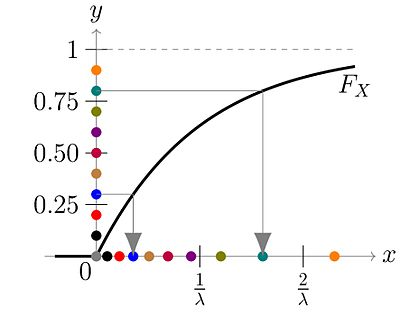
\includegraphics[scale=0.6]{./images/sampling/inverse.jpg}
	\end{center}
	\caption{$y$-axis: Uniform distribution, $x$-axis: sample value}
\end{figure}

\begin{figure}[t]
	\begin{center}
		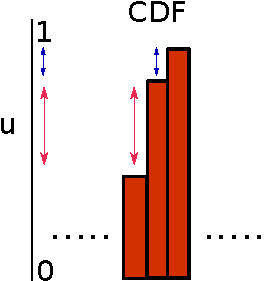
\includegraphics[scale=1.2]{./images/sampling/cdf.pdf}
	\end{center}
	\caption{How can this sampling method recover the original distribution?}
\end{figure}

\subsection{Ancestral Sampling}
$$p(\mathbf{x}) = p(\mathbf{x}_1)p(\mathbf{x}_2|\mathbf{x}_1)p(\mathbf{x}_3|\mathbf{x}_2)\cdots$$
Sampling steps:
\begin{enumerate}
	\item sample $\mathbf{x}_1$
	\item sample $\mathbf{x}_2$ conditioned by $\mathbf{x}_1$
	\item sample $\mathbf{x}_3$ conditioned by $\mathbf{x}_2$
\end{enumerate}



\subsection{Rejection Sampling}
Rejection sampling is a simple method. It rejects samples violating a given condition (\eg conditions of conditional probability.). Let's see its theory. 

Rejection sampling is a method for sampling from a distribution $p(x)=\frac{1}{Z}p'(x)$ that is difficulut to sample directly, but its unnormalized pdf $p'(x)$ is east to evaluate ($Z$ is hard to compute). In rejection sampling, we need some simpler distribution $q(x)$, called a \textbf{proposal distribution}. 

The intuition of rejection sampling is actually similar to Monte-Carlo estimation. By setting a large area (proposal distribution), we can sample points and take them that are inside the our target distribution

% The $k$ must be sufficiently large to envelope the true distribution.
To run the rejection sampling, introduce a constant $k$ whose value is chosen such that $kq(x)\geq p'(x)$ for all values of $x$. The function $kq(x)$ is called a comparison function. Each step of the rejection sampler involves generating two random variables:
	\begin{enumerate}
		\item Sample $x_0\sim q$
		\item Sample $u_0\sim U[0,kq(x_0)]$.
	\end{enumerate}
	Finally, If $u_0>p'(x_0)$, then the sample $x_0$ will be rejected, otherwise we add the sample $x_0$ to our set of samples $\{x^{r}\}$.

	\begin{figure}[h]
		\begin{center}
			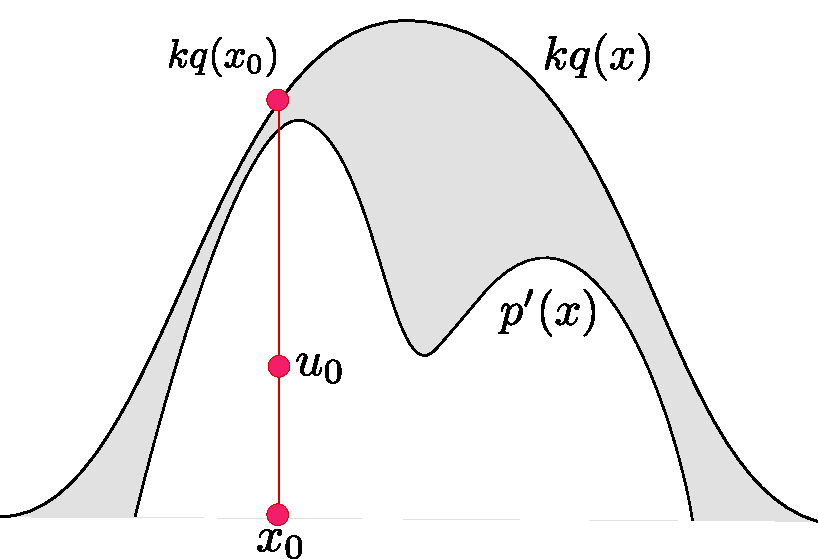
\includegraphics[scale=0.5]{./images/sampling/rejection.pdf}
		\end{center}
	\end{figure}

	The original values of $x$ are generated from the distribution $q(x)$ and these samples are then accepted with probability $p'(x)/kq(x)$ (see the figure above. The acceptance probability (\ie length) is the $p'$ divided by $kq$). Then, the probability that a sample will be accepted is given by   
	\begin{align*}
	p(accept) &= p\Bigg(u\leq \frac{p'(x)}{kq(x)}\Bigg)\\
	&= \int p\Bigg(u\leq \frac{p'(x)}{kq(x)}\bigg|x\Bigg)q(x)dx\\
	% & = \mathbb{E}[p'(x)/kq(x)] \tiny \textrm{ by Lemma 1} \\
	& = \int \frac{p'(x)}{kq(x)}q(x)dx\\
	& = \frac{1}{k}\int p'(x)dx
	\end{align*}
	Thus, the sampling will be more efficient if we choose small $k$ to increase the change of acceptance. 
%	\begin{align*}
%	p(accpet) &= \int p(accpet, x)dx\\
%	& = \int \frac{p'(x)}{kq(x)}q(x)dx\\
%	& = \frac{1}{k}\int p'(x)dx\\
%	& = \frac{1}{k}
%	\end{align*}
%	\begin{align*}
%		p(x^*) &= \frac{[p'(x^*)/kq(x^*)]q(x^*)}{\int [p'(x)/kq(x)]q(x)dx}\\
%		& = \frac{p'(x^*)}{\int p'(x^*)dx}\\
%		& = p(x^*)
%	\end{align*}

\subsection{Importance Sampling}

We want to estimate an expectation of function $f(x), x\sim p(x)$, but it would be hard to estimate the distribution $p(x)$. Again, the importance sampling is not a method for generating samples from $p(\mathbf{x})$. In this case, we can use a simple distribution $q(x)$ by
$$\mathbb{E}(f) = \int f(x)p(x)dx = \int f(x)\frac{p(x)}{q(x)}q(x)dx \approx \frac{1}{N}\sum_{n=1}^N \frac{p(x_i)}{q(x_i)}f(x_i) .$$

%Importance sampling is not a method for generating samples from $p(\mathbf{x})$. It is just a method for estimating the expectation of a function $f(\mathbf{x})$. We first generate $R$ samples $\{x^{(r)}\}$ from $q(x)$, then we could estimate the expectation by Monte Carlo method. However, if the generated samples, values of $x$ where $q(x)$ is greater than $p(x)$ will be over-represented in this estimator, and where $q(x)$ is less than $p(x)$ will be under-represented. Thus, we introduce weights 
%$$w_r = \frac{p(x^*)}{q(x^*)}$$
	
%	%$$\hat{f} = \frac{1}{L}\sum_{l=1}^{L}f(\mathbf{z}^{(l)})$$

\begin{itemize}
	\item Assume that $p(\mathbf{x})$ is known and too complicated to be sampled directly. 
	\item Samples are independently drawn from a \textbf{proposal density} $Q(\mathbf{x})$, which is designed to be close to the true density $p(\mathbf{x})$ and \textbf{simpler}
	\item Generate $R$ samples from $Q(\mathbf{x})$
\end{itemize}

\section{Gibbs Sampling}
% \label{sec:}

The phrase ``Markov chain Monte Carlo'' encompasses a broad array of techniques that have in common a few key ideas. The setup for all the techniques that we will discuss in this book is as follows:

\begin{enumerate}
	\item We want to sample from a some complicated density or probability mass function $\pi$. Often, this density is the result of a Bayesian computation so it can be interpreted as a posterior density. The presumption here is that we can evaluate $\pi$ but we cannot sample from it.
	\item We know that certain stochastic processes called Markov chains will converge to a stationary distribution (if it exists and if specific conditions are satisfied). Simulating from such a Markov chain for a long enough time will eventually give us a sample from the chain’s stationary distribution.
	\item Given the functional form of the density $\pi$, we want to construct a Markov chain that has $\pi$ as its stationary distribution.
	\item We want to sample values from the Markov chain such that the sequence of values $\{x_n\}$ generated by the chain converges in distribution to the density $\pi$.
\end{enumerate}

In order for all these ideas to make sense, we need to first go through some background on Markov chains. The rest of this chapter will be spent defining all these terms, the conditions under which they make sense, and giving examples of how they can be implemented in practice.

\subsection{Markov Chain}

A Markov chain is a stochastic process that evolves over time by transitioning into different states. The sequence of states is denoted by the collection $\{X_i\}$ and the transition between states is random, following the rule 
$$P(X_t|X_{t-1},\dots,X_0)=P(X_t|X_{t-1})$$

\begin{itemize}
	\item Each node has a probability distribution of states.
	\item Each link represents a probability state transition.  
		% \begin{align*}
		% 	P(X_1=i) = \sum_{i=1}^N P(X_i=j|X_0=i)P(X_0=i)\\
		% \end{align*}
\end{itemize}

\begin{itemize}
	\item $i \to j$: Accessible if a state $j$ is accessible from $i$. 
		\begin{itemize}
			\item $i \leftrightarrow j$: Communicate between the two states.
		\end{itemize}
	\item Reducibility: A Markov chain is \textbf{\textit{irreducible}} if $i\leftrightarrow j, \forall i,j\in S$. Simply, if all states can visit other states, then it is irreducible. 
	\item Periodic: State $i$ has a period $d$ (\ie periodically visit the state $i$) $\leftrightarrow$ aperiodic.
	\item Transience: A state is transient if, when we leave this state, there is a non-zero probability that we will never return to it. Conversely, a state is recurrent if we know that we will return to that state, in the future, with probability 1 after leaving it (if it is not transient). 
		\begin{itemize}
			\item Stationary Distribution: A probability of being in a state s at time-step t is equal to a probability of being in the state s at the next time-step. Then, it is a stationary probability distribution.
		\end{itemize}
	\item Ergodicity: A state is ergodic if the state is recurrent, aperiodic. Markov chain is ergodic if all states are ergodic. 
\end{itemize}

\subsection{Stationary Distribution}
% The return time $RT_i = \min\{n>0: X_n=i|X_0=i\}$ is the minimum time when we observe the state $X_n$ is at $i$ after the first visit ($X_0$) at $n$. 

% Limit theorem of Markov chain:
% \begin{itemize}
% 	\item If a MC is irreducible and ergodic.
% \end{itemize}

\paragraph{Limit theorem of Markov chain}

For a Markov chain with a discrete state space and transition matrix $P$, let $\pi_*$ be such that $\pi_*P=\pi_*$. Then $\pi_*$ is a stationary distribution of the Markov chain and the chain is said to be stationary if it reaches this distribution.

The basic limit theorem for Markov chains says that, under a specific set of assumptions that we will detail below, we have 
$$||\pi_*-\pi_n|| \to 0$$
as $n\to\infty$, where $||\cdot||$ is the total variation distance between the two densities. Therefore, no matter where we start the Markov chain ($\pi_0$), $\pi_n$ will eventually approach the stationary distribution. Another way to think of this is that 
$$\lim_{n\to\infty}\pi_n(i)=\pi_*(i).$$
for all states $i$ in the state space. Note that $\pi_0$ is the probability distribution of the Markov chain at time 0. Also, $\pi_n$ denote the distribution of the chain at time $n$.

\url{https://bookdown.org/rdpeng/advstatcomp/background.html}


\paragraph{Reversible MC}
Consider a stationary ergodic Markov chain with transition probability$p(i, j)$ and stationary distribution $\pi(i)$, if we reverse the process, we will get a reversed Markov chain with transition probability$q(i, j)$: 
\begin{align*}
	q(j,i) &= P(X_m=i|X_{m+1}=j)\\
		   &= \frac{P(X_m=i,X_{m+1}=j)}{P(X_{m+1}=j)}\\
		   &= \frac{P(X_m=i|X_{m+1}=j)P(X_{m+1}=j)}{P(X_{m+1}=j)}\\
		   &= \frac{\pi(i)p(i,j)}{\pi(j)}\\
	\pi(i)p(i,j) &= \pi(j)q(j,i)
\end{align*}
If $p(i,j) = q(j,i)$, it is called time-reversible Markov chain. 

% \section{Markov Chain for Sampling}


\section{Markov Chain Monte Carlo}
MCMC aims to generate samples from some complex probability distribution $p(x)$ that is difficult to directly sample from.

The basic sampling methods we have learnt so far do not leverage past information, which assumes all samples are independent. In Markov chain based sampling, we will treat random variables as a sequence of sampling process. 

In Markov Chain Monte Carlo(MCMC), we assume that a stationary distribution is already known. We are more interested in estimating a transition rule that describing the stationary distribution. 



Ground rules for MCMCs:
\begin{itemize}
	\item MCMCs stochastically explore the parameter space in such a way that the histogram of their samples produces the target distribution.
	\item Markovian: Evolution of the chain (\ie collections of samples from one iteration to the other) only depends on the current position and some transition probability distribution (\ie how we move from one point in parameter space to another). This means that the chain has no memory and past samples cannot be used to determine new positions in parameter space.
	\item The chain will converge to the target distribution if the transition probability is:
		\begin{itemize}
			\item Irreducible: From any point in parameter space, we must be able to reach any other point in the space in a finite number of steps.
			\item Positive recurrent: For any point in parameter space, the expected number of steps for the chain to return to that point is finite. This means that the chain must be able to re-visit previously explored areas of parameter space.
			\item Aperiodic: The number of steps to return to a given point must not be a multiple of some value $k$. This means that the chain cannot get caught in cycles.
		\end{itemize}
\end{itemize}



\subsection{Metropolis-Hasting Algorithm}
% \begin{itemize}
% 	\item Current value $z^t$
% 	\item Propose a candidate $z^*\sim q(z^*|z^t)$ where $q_t$ is a proposal distribution (\ie Normal distribution). 
% 	\item Same as importance and rejections samplings, yet the difference is the Markov property idea in the proposal distribution. 
% 	\item With an acceptance probability (or moving criteria), $\alpha$.
% \end{itemize}

% \href{https://youtu.be/oX2wIGSn4jY}{Ref: YouTube Lecture}

% % The product of MCMC is a posterior distribution.

Suppose we have a target posterior distribution $\pi(x)$, where $x$ here can be any collection of parameters (not a single parameter). In order to move around this parameter space we must formulate some proposal distribution:

$$q(x_{i+1}\mid x_i),$$

that specifies the probability of moving to a point in parameter space, $x_{i+1},$ given that we are currently at $x_i$. The Metropolis Hastings algorithm accepts a ``jump'' to $x_{i+1}$ with the following probability

$$\kappa(x_{i+1}\mid x_i) = \mathrm{min}\left(1, \frac{\pi(x_{i+1})q(x_i\mid x_{i+1})}{\pi(x_{i})q(x_{i+1}\mid x_{i})}\right) = \mathrm{min}(1, H),$$

where the fraction above is called the Hastings ratio, $H$. The above expression represents that the probability of transitioning from point $x_{i+1}$ given the current position $x_{i}$ is a function of the ratio of the value of the posterior at the new point to the old point (\ie $\pi(x_{i+1})/\pi(x_i)$) and the ratio of the transition probabilities at the new point to the old point (\ie $q(x_i\mid x_{i+1})/q(x_{i+1}\mid x_i)$). Firstly, it is clear that if the ratio is bigger than 1 then the jump will be accepted. Secondly, the ratio of the target posteriors ensures that the chain will gradually move to high probability regions. Lastly, the ratio of the transition probabilities ensures that the chain is not ``favored'' toward certain locations by the proposal distribution function. Note that many proposal distributions are symmetric (\ie $q(x_{i+1}\mid x_i) = q(x_i\mid x_{i+1})$).

The Metropolis-Hasting algorithm is then:

\begin{lstlisting}[language=Python]
def mh_sampler(x0, lnprob_fn, prop_fn, prop_fn_kwargs={}, iterations=100000):
    """Simple metropolis hastings sampler.

    :param x0: Initial array of parameters.
    :param lnprob_fn: Function to compute log-posterior.
    :param prop_fn: Function to perform jumps.
    :param prop_fn_kwargs: Keyword arguments for proposal function
    :param iterations: Number of iterations to run sampler. Default=100000

    :returns:
        (chain, acceptance, lnprob) tuple of parameter chain , acceptance rate
        and log-posterior chain.
    """

    # number of dimensions
    ndim = len(x0)

    # initialize chain, acceptance rate and lnprob
    chain = np.zeros((iterations, ndim))
    lnprob = np.zeros(iterations)
    accept_rate = np.zeros(iterations)

    # first samples
    chain[0] = x0
    lnprob0 = lnprob_fn(x0)
    lnprob[0] = lnprob0

    # start loop
    naccept = 0
    for ii in range(1, iterations):

        # propose
        x_star, factor = prop_fn(x0, **prop_fn_kwargs)

        # draw random uniform number
        u = np.random.uniform(0, 1)

        # compute hastings ratio
        lnprob_star = lnprob_fn(x_star)
        H = np.exp(lnprob_star - lnprob0) * factor

        # accept/reject step (update acceptance counter)
        if u < H:
            x0 = x_star
            lnprob0 = lnprob_star
            naccept += 1

        # update chain
        chain[ii] = x0
        lnprob[ii] = lnprob0
        accept_rate[ii] = naccept / ii

    return chain, accept_rate, lnprob

\end{lstlisting}


% \begin{algorithm}
% 	Initialization: $x_0$\\
% 	\For {$i=1,\dots,N$}{
		
% 	}
% 	Return $p(X) = \sum_i^M \alpha_T^i$
% 	\caption{Metropolis-Hasting algorithm}
% 	\label{algo:metro-polis}
% \end{algorithm}




\chapter{Topic Modeling}
\section{Latent Dirichlet Allocation}
\label{sec:topic_modeling_lda}


The assumptions of LDA:
\begin{itemize}
	\item Each topic is a distribution over words.
	\item Each document is a mixture of corpus-wide topics.
	\item Each word is sampled from one of topics. 
\end{itemize}
The LDA attempts to model the document generation process stochastically. However, we have to infer the latent structure (the distributions) of documents. 

\begin{figure}[h]
	\centering
	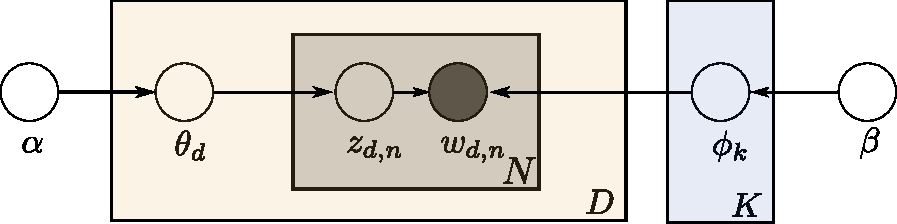
\includegraphics[scale=1.0]{./images/lda/lda.pdf}
\end{figure}
\begin{itemize}
	\item $\theta_d\sim Dir(\alpha)$: For each document, draw topic distribution. 
		\begin{itemize}
			\item $\alpha$: Dirichlet parameter
		\end{itemize}
	\item $z_{d,n}\sim Mult(\theta_d)$: per-word topic assignment. The $n$-th word of document $d$ is from which topic?
	\item $w_{d,n}\sim Mult(\phi_{z_{d,n}},n)$: observed word. The $n$-th word in a document $d$ is from a certain topic ($z_{d,n}$) distribution $\phi_{z_{d,n}}$.
	\item $\phi_k\sim Dir(\beta), i=\{1,\dots,K\}$: topics.
		\begin{itemize}
			\item $\beta$: topic hyperparameter (Dirichlet parameter).
		\end{itemize}
\end{itemize}
The document generation process can be modelled as follows:
\begin{align*}
	p(\phi_{1:K}, \theta_{1:D}, z_{1:D}, w_{1:D}) = \prod_{i=1}^K p(\phi_i|\beta)\prod_{d=1}^D p(\theta_d|\alpha)\bigg(\prod_{n=1}^N p(w_{d,n}|\phi_{1:K},z_{d,n})p(z_{d,n}|\theta_d)\bigg).
\end{align*}

\subsection{LDA Inference}
The posterior of the latent variables given the document is
\begin{align*}
	p(\phi, \theta, \mathbf{z}|\mathbf{w}) = \frac{p(\phi, \theta, \mathbf{z},\mathbf{w})}{\int_{\phi}\int_{\theta}\sum_{\mathbf{z}}p(\phi, \theta, \mathbf{z},\mathbf{w})}
\end{align*}
\begin{itemize}
	\item The denominator is intractable
\end{itemize}
We want to estimate the topic distribution $\mathbf{z}$. 

\subsection{Dirichlet Distribution}
The Dirichlet Distribution can be considered as a extension of the beta distribution. 
\begin{align}
	p(P=\{p_i\}|\alpha_i) = \frac{\Gamma(\sum_i\alpha_i)}{\prod_i\Gamma(\alpha_i)}\prod_ip_i^{\alpha_i-1}
	\label{eq:dirichlet_dist}
\end{align}
\begin{itemize}
	\item $\sum_ip_i = 1$
	\item The posterior distribution of Dirichlet distribution is also Dirichlet distribution. 
\end{itemize}


% \part{Introduction to Machine Learning}
\chapter{Latent Variable Models}
\section{Introduction}
\subsection{Motivation of Latent Variable Models}
\label{sec:intro_motivation}
If we knew a corresponding latent variable for each observation, then modelling might be easier. Imagine, how can we find $z^* = \argmax_{z} p(\mathbf{x|z})$ for the data $\mathbf{x}$ as shown in Fig. \ref{fig:clusters}(b)

\begin{figure}[h]
	\begin{center}			
		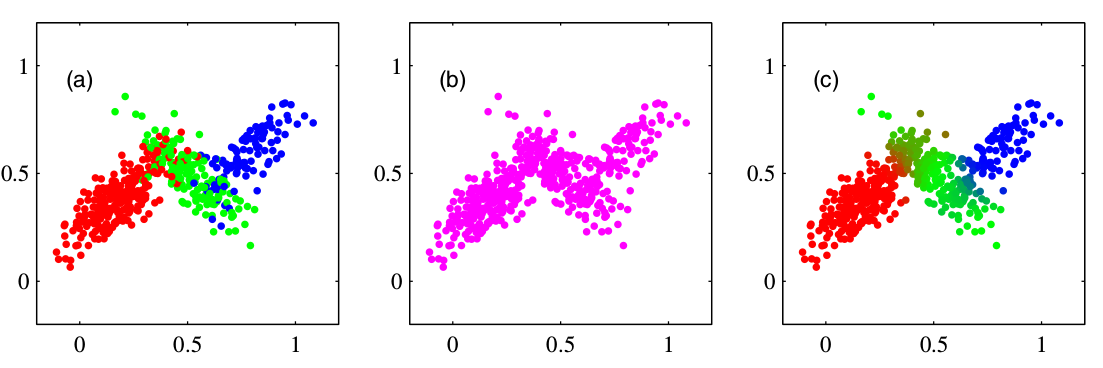
\includegraphics[scale=0.25]{./images/generative/latent.png}
	\end{center}
	\caption{(a) Complete data set $p(\mathbf{x|z})$. (b) Incomplete data set $p(\mathbf{x})$. (c) Inference result}
	\label{fig:clusters}
\end{figure}
For example, we want to model the complete data set $p(\mathbf{x|z})$ under the i.i.d. assumption 
\begin{equation*}
p(\mathbf{x}_i, \mathbf{z}_i|\boldsymbol{\theta}) = 
\begin{cases}
p(\mathcal{C}_1)p(\mathbf{x}_i|\mathcal{C}_1) \textrm{ if } z_i=0\\
p(\mathcal{C}_2)p(\mathbf{x}_i|\mathcal{C}_2) \textrm{ if } z_i=1\\
p(\mathcal{C}_3)p(\mathbf{x}_i|\mathcal{C}_3) \textrm{ if } z_i=2\\
\end{cases}
\end{equation*}
\begin{align*}
p(\mathbf{x}_1, \mathbf{x}_2,...,\mathbf{x}_N, \mathbf{z}_1, \mathbf{z}_2, ..., \mathbf{z}_N|\boldsymbol{\theta}) = \prod_{n=1}^{N}\prod_{k=1}^{K}\pi_k^{z_{nk}}\mathcal{N}(\mathbf{x}_n|\boldsymbol{\mu}_k, \boldsymbol{\Sigma}_k)^{z_{nk}}
\end{align*}
, where $\pi_k=p(\mathcal{C}_k)$ and $p(\mathbf{x}_i|\mathcal{C}_k)=\mathcal{N}(\mathbf{x}_n|\boldsymbol{\mu}_k, \boldsymbol{\Sigma}_k)$. However, in many cases, it is not observable. 

%In this case, what we can only do is find a posterior $p(\mathbf{x}|\mathbf{z},\boldsymbol{\theta})$.

\chapter{Clustering}


\section{K-Means Clustering}
Suppose we have a data set $\mathbf{X} = \{\mathbf{x}_1,...,\mathbf{x}_n\}$ consisting of $N$ observations of a random $D$-dimensional variable $\mathbf{x}\in \mathbb{R}^{D}$. Our goal is to partition the data into some number $K$ of clusters.  Intuitively, we may think of a cluster as comprising a group of data points whose inter-point distances are small compared with the distances to points outside of the cluster.

This notion can be formalized by introducing a set of $D$-dimensional vectors $\boldsymbol{\mu}_k$, which represents the centers of the clusters. Our goal is to find an assignment of data points to clusters, as well as a set of vectors $\{\boldsymbol{\mu}_k\}$. Objective function of $K$-means clustering (\textit{distortion measure}) can be defined as follows:
$$J =  \sum_{n=1}^{N}\sum_{k=1}^{K}r_{nk}||\boldsymbol{x}_n-\boldsymbol{\mu}_k||^2$$
, where $r_{nk}\in\{0,1\}$ is a binary indicator variable which represents the \textbf{membership of data} $\mathbf{x}_n$. Our goal is to find values for the $\boldsymbol{\mu}_k$ and the $r_{nk}$ so as to minimize $J$. 

We can minimize $J$ through an iterative procedure in which each iteration involves two successive steps corresponding to successive optimizations with respect to the $\boldsymbol{\mu}_k$ and the $r_{nk}$ First we choose some initial values for the $\boldsymbol{\mu}_k$. Then in the first phase we minimize $J$ with respect to the $r_{nk}$, keeping the $\boldsymbol{\mu}_k$ fixed. In the second phase we minimize $J$ with respect to the $\boldsymbol{\mu}_k$, keeping $r_{nk}$ fixed. This two-stage optimization is then repeated until convergence.

The $r_{nk}$ can be optimized in a closed-form solution as follows:
$$r_{nk}=\begin{cases}
1 & \textrm{if } k=\argmin_{j} ||\boldsymbol{x}_n-\boldsymbol{\mu}_j||^2\\
0 & \textrm{otherwise}
\end{cases}$$

Now consider the optimization of the $\boldsymbol{\mu}_k$ with the $r_{nk}$ held fixed. The objective function $J$ is a quadratic function of $\boldsymbol{\mu}_k$, and it can be minimized by setting its derivative with respect to $\boldsymbol{\mu}_k$ to zero giving
\begin{align*}
2\sum_{n=1}^{N}r_{nk}(\boldsymbol{x}_n-\boldsymbol{\mu}_k) = 0.
\end{align*}
We can arrange as
\begin{align*}
\boldsymbol{\mu}_k = \frac{\sum_n r_{nk}\boldsymbol{x}_n}{\sum_n r_{nk}}.
\end{align*}

% \begin{enumerate}
% 	\item Expectation (expectation of a log-likelihood give parameters): $$2\sum_{n=1}^{N}r_{nk}(\boldsymbol{x}_n-\boldsymbol{\mu}_k) = 0.$$
% 	\item Maximization (maximize parameters give a log-likelihood function): $$\boldsymbol{\mu}_k = \frac{\sum_n r_{nk}\boldsymbol{x}_n}{\sum_n r_{nk}}.$$ This updates the centroids. 
% \end{enumerate}

The denominator of $\boldsymbol{\mu}_k$ is equal to the number of points assigned to cluster $k$. The mean of cluster $k$ is essentially the same as the mean of data points $\mathbf{x}_n$ assigned to cluster $k$. For this reason, the procedure is known as the $K$-means clustering algorithm. 

The two phases of re-assigning data points to clusters and re-computing the cluster means are repeated in turn until there is no further change in the assignments. These two phases reduce the value of the objective function $J$, so the convergence of the algorithm is assured. However, it may converge to a local rather than global minimum of $J$. 

Some properties:
\begin{itemize}
	\item Hard clustering ($\leftrightarrow$ Soft clusstering)
	\item Centroid initialization issue.
	\item The number of clusters is uncertain. 
	\item Distance metric issue (\eg Euclidean?)
\end{itemize}



\newpage
\section{Gaussian Mixture Models}

\subsection{Multinomial Distribution}
$$P(X|\boldsymbol{\mu}) = \prod_{n} \prod_k \mu_k^{x_{nk}} = \prod_k\mu_k^{\sum_n x_{nk}}.$$
How to determine the MLE solution of $\boldsymbol{\mu}?$ \ie maximize$P(X|\boldsymbol{\mu})$ subject to $\mu_k\geq 0$ and $ \sum_k \mu_k = 1$. We can use the Lagrange method. 

\begin{align*}
	&\mathcal{L} = \sum_k\sum_nx_{nk}\ln \mu_k +\lambda(\sum_k\mu_k-1)\\ 
	&\frac{\partial \mathcal{L}}{\partial \mu_k} = \frac{\sum_nx_{nk}}{\mu_k}+\lambda. \\
	& \mu_k^{\textrm{ML}} = \frac{m_k}{N},
\end{align*}
where $m_k = \sum_n x_{nk}.$ We can consider the joint distribution of the quantities $m_1, \dots, m_K$, conditioned on the parameters $\boldsymbol{\mu}$ and on the total number $N$ observations: 
$$\textrm{Mult}(m_1, \dots, m_K|\boldsymbol{\mu}, N) = \binom{N}{m_1, \dots, m_K} = \frac{N!}{m_1!,\dots, m_K!}.$$
Note that the variables $m_k$ are subject to the constraint
$$\sum_k m_k = N.$$


\subsection{Multivariate Gaussian Distribution}
\begin{align*}
	\mathcal{N}(x|\mu,\sigma^2) = \frac{1}{\sqrt{2\pi\sigma^2}}\exp\bigg(-\frac{1}{2\sigma^2}(x-\mu)^2\bigg)
\end{align*}
For a $D$-dimensional vector $\mathbf{x}$, 
\begin{align*}
	\mathcal{N}(\mathbf{x}|\boldsymbol{\mu},\boldsymbol{\Sigma}) &= \frac{1}{(2\pi)^{D/2}|\boldsymbol{\Sigma}|^{1/2}}\exp\bigg(-\frac{1}{2}(\mathbf{x}-\boldsymbol{\mu})^T\boldsymbol{\Sigma}^{-1}(\mathbf{x}-\boldsymbol{\mu})\bigg)\\
	\ln\mathcal{N}(\mathbf{x}|\boldsymbol{\mu},\boldsymbol{\Sigma}) &= -\frac{1}{2}\ln|\boldsymbol{\Sigma}|-\frac{1}{2}(\mathbf{x}-\boldsymbol{\mu})^T\boldsymbol{\Sigma}^{-1}(\mathbf{x}-\boldsymbol{\mu})+C.
\end{align*}
Note that the functional dependence of the Gaussian on $\mathbf{x}$ is through the quadratic form: 
$$\Delta^2 = (\mathbf{x}-\boldsymbol{\mu})^T\boldsymbol{\Sigma}^{-1}(\mathbf{x}-\boldsymbol{\mu}).$$
The quantity $\Delta$ is called the \textit{Mahalanobis distance} from $\boldsymbol{\mu}$ to $\mathbf{x}$ and reduces to the Euclidean distance when $\boldsymbol{\Sigma}$ is the identity matrix.

Also,by using i.i.d. condition of a dataset, we can also express as follows:
\begin{align*}
	\ln\mathcal{N}(\mathbf{X}|\boldsymbol{\mu},\boldsymbol{\Sigma}) &= -\frac{N}{2}\ln|\boldsymbol{\Sigma}|-\frac{1}{2}\sum_n(\mathbf{x}_n-\boldsymbol{\mu})^T\boldsymbol{\Sigma}^{-1}(\mathbf{x}_n-\boldsymbol{\mu})+C
\end{align*}








\subsection{Gaussian Mixture Models}


K-means clustering is a hard-clustering, but in some cases soft-clustering provides a better model in practice. Gaussian mixture model assumes a simple \textbf{linear superposition} of Gaussian components, aimed at providing a richer class of density models than the single Gaussian. Let's consider a single sample case and it can be expressed as follows:
$$p(\mathbf{x})= \sum_{k=1}^{K}\pi_k\mathcal{N}(\mathbf{x}|\boldsymbol{\mu_k}, \boldsymbol{\Sigma}_k)$$
Let us introduce a $K$-dimensional binary random variable $\mathbf{z}$ having a 1-of-$K$ representation in which a particular element $z_k$ is equal to 1 and all other elements are 0. I will explain more about $\mathbf{z}$ later. It satisfied the following properties:
\begin{itemize}
	\item $z_k\in\{0,1\}$
	\item $\sum_kz_k=1$
\end{itemize}
The marginal distribution over $\mathbf{z}$ is specified in terms of the mixing coefficients $\pi_k$, such that 
$$p(z_k=1) = \pi_k$$
, where the mixing coefficients must satisfy
$$0\leq\pi_k\leq1$$
and 
$$\sum_{k=1}^{K}\pi_k = 1 $$
in order to be valid probabilities. We can also write pdf of $\mathbf{z}$ in a product of mixing coefficient because it is a 1-of-$K$ representaion.
$$p(\mathbf{z}) = \prod_{k=1}^{K}\pi_k^{z_k} = \pi_k \because z_k\in\{
0,1\}$$
Similarly, the conditional distribution of $\mathbf{x}$ given a particular $\mathbf{z}$ can be modeled to be a Gaussian distribution.
\begin{equation*}
p(\mathbf{x}|z_k=1) = \mathcal{N}(\mathbf{x}|\boldsymbol{\mu}_k, \boldsymbol{\Sigma}_k) 
\end{equation*}
Also can be represented in the form 
\begin{align*}
p(\mathbf{x}|\mathbf{z}) &= \prod_{k=1}^{K}\mathcal{N}(\mathbf{x}|\boldsymbol{\mu}_k, \boldsymbol{\Sigma}_k)^{z_k}\\
& = \mathcal{N}(\mathbf{x}|\boldsymbol{\mu}_k, \boldsymbol{\Sigma}_k) \because z_k\in\{
0,1\}
\end{align*}
Finally, marginal data distribution can be obtrained by summing the joint distribution over all possible states of $\mathbf{z}$ to give
\begin{align*}
	p(\mathbf{x}) &  = \sum_{\mathbf{z}} p(\mathbf{x},\mathbf{z})\\
	& = \sum_{\mathbf{z}} p(\mathbf{z})p(\mathbf{x}|\mathbf{z})= \sum_{z_1,...,z_K} p(z_1,...,z_K)p(\mathbf{x}|z_1,...,z_K)\\
	& = \sum_{k=1}^{K}\pi_k \mathcal{N}(\mathbf{x}|\boldsymbol{\mu}_k, \boldsymbol{\Sigma}_k) 
\end{align*}
Note that for every observed data point $\mathbf{x}_n$ there is a corresponding latent variable $\mathbf{z}_n$, which \textbf{indicates the membership of} $\mathbf{x}_n$. This can be represented as in Fig. \ref{fig:gmm}.

\begin{figure}[h]
	\begin{center}			
		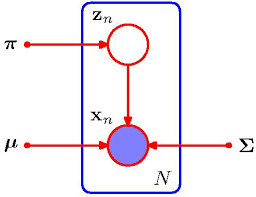
\includegraphics[scale=0.4]{./images/generative/gmm.png}
	\end{center}
	\caption{Graphical representation of GMM model. The GMM models a joint distribution $p(\mathbf{x}, \mathbf{z})$ in terms of a marginal distribution $p(\mathbf{z})$ and conditional distribution $p(\mathbf{x}|\mathbf{z})$ to model $p(\mathbf{x})$. Each $\mathbf{x}_n$ is coupled with $\mathbf{z}_n$}
	\label{fig:gmm}
\end{figure}
Now we can work with the joint distribution $p(\mathbf{x,z})$ instead of the marginal distribution $p(\mathbf{x})$, which is hard to estimate directly as explained in \Cref{sec:intro_motivation}. 

Another quantity which plays a central role is the conditional proability of $\mathbf{z}$ given $\mathbf{x}$, $p(z_k=1|\mathbf{x})$. 
\begin{itemize}
\item $p(z_k=1) = \pi_k$ can be viewed as a prior of $z_k=1$
\item $\gamma(z_k)$: assignment probability or responsibility. This represents the probability of assignment of a sample.  This quantity will be updated through the Bayes Theorem.
\item[] $\rightarrow$  A simple explanation is that \textbf{this is the classification result} of $\mathbf{x}_n$.
\end{itemize}
\begin{align*}
\gamma(z_k) \equiv p(z_k=1|\mathbf{x}) & \equiv \frac{p(z_k=1)p(\mathbf{x}|z_k=1)}{\sum_{j=1}^{K}p(z_j=1)p(\mathbf{x}|z_j=1)} \\
& = \frac{\pi_k\mathcal{N}(\mathbf{x}|\boldsymbol{\mu}_k, \boldsymbol{\Sigma}_k)}{\sum_{j=1}^{K} \pi_j\mathcal{N}(\mathbf{x}|\boldsymbol{\mu}_j, \boldsymbol{\Sigma}_j)}
\end{align*}

\subsection{Maximum Likelihood}
Suppose we have a data set of observations $\mathbf{X}=\{\mathbf{x}_1,...,\mathbf{x}_n\}^{T}\in\mathbbm{R}^{N\times D}$ and we want to model the data distribution $p(\mathbf{X})$ using GMM. If we assume an \textrm{i.i.d.} data set, it can be expressed as follows: 
\begin{align*}
p(\mathbf{X}|\boldsymbol{\pi},\boldsymbol{\mu},\boldsymbol{\Sigma}) &=\prod_{n=1}^{N}\Bigg(\sum_{k=1}^{K}\pi_k\mathcal{N}(\mathbf{x}_n|\boldsymbol{\mu}_k, \boldsymbol{\Sigma}_k)\Bigg)\\
\end{align*}
then its \textbf{loglikelihood function for GMM} is given by:
\begin{align*}
\ln p(\mathbf{X}|\boldsymbol{\pi},\boldsymbol{\mu},\boldsymbol{\Sigma}) &= \sum_{n=1}^{N}\ln \Bigg(\sum_{k=1}^{K}\pi_k\mathcal{N}(\mathbf{x}_n|\boldsymbol{\mu}_k, \boldsymbol{\Sigma}_k)\Bigg)
\end{align*}

%In a single dimension case, 
%\begin{align*}
%	\ln p(x, \pi, \mu, \sigma) & =\sum_{n=1}^{N}\ln \sum_{k=1}^{K}\pi_k \frac{1}{\sigma_k \sqrt{2\pi_k}}\exp\Big(-\frac{1}{2}\Big(\frac{x_n-\mu_k}{\sigma_k}\Big)^2\Big)\\
%	\frac{\partial }{\partial \mu_k}\ln p(x, \pi, \mu, \sigma) & =\sum_{n=1}^{N} \frac{\pi_k \frac{1}{\sigma_k \sqrt{2\pi}}\exp\Big(-\frac{1}{2}\Big(\frac{x_n-\mu_k}{\sigma_k}\Big)^2\Big) \frac{x_n-\mu_k}{\sigma_k^2}}{\sum_{k=1}^{K}\pi_k \frac{1}{\sigma_k \sqrt{2\pi}}\exp\Big(-\frac{1}{2}\Big(\frac{x_n-\mu_k}{\sigma_k}\Big)^2\Big)}\\
%	& =\sum_{n=1}^{N} \underbrace{\frac{\pi_k \mathcal{N}(x_n|\mu_k, \sigma_k) }{\sum_{k=1}^{K}\pi_k \mathcal{N}(x_n|\mu_k, \sigma_k)}}_{=\gamma(z_{nk})}\frac{x_n-\mu_k}{\sigma_k^2}\\
%	\mu_k &=\frac{1}{N_k}\sum_{n=1}^{N} \gamma(z_{nk}) x_n,
%\end{align*}
%where 
%$N_k = \sum_{n=1}^{N} \gamma(z_{nk})$. $N_k$ can be interpreted as the effective number of points assigned to cluster $k$. 

How to solve this MLE? While a gradient-based optimization is possible, we consider the iterative \textit{Expectation Maximization} algorithm.

Before, maximizing the likelihood, it is worth to emphasize two issues in GMM: (i) \textit{singularities} and (ii) \textit{identifiability}.

%\subsection{Singularity and Identifiability}
\paragraph{Singularity}
% Suppose that one of the components of the mixture model, let us say the $j$-th component, has its mean $\mathbf{\mu}_j$ exactly equal to one of the data points so that $\mathbf{\mu}_j=\mathbf{x}_n$ for some value of $n$. This data point will then contributes a term in the likelihood function of the form 
% $$\mathcal{N}(\mathbf{x}_n, \sigma_j^2\mathbf{I}) = \frac{1}{(2\pi)^{1/2}} \frac{1}{\sigma_j}$$
% If we consider the limit $\sigma_j \to 0$, then we see that this term goes to infinity and so the log likelihood function will also go to infinity. Thus the maximization of the log likelihood function will also go to infinity. Thus the maximization of the log likelihood function is not a well posed problem because such sigularities will walways be present and will occur whenever one of the Gaussian components collapses onto a specific data point. 

Before discussing how to maximize this function, it is worth emphasizing that there is a significant problem associated with the maximum likelihood framework applied to Gaussian mixture models, due to the presence of singularities. For simplicity, consider a Gaussian mixture whose components have covariance matrices given by $\Sigma_k = \sigma^2_kI$, where $I$ is the unit matrix, although the conclusions will hold for general covariance matrices. Suppose that one of the components of the mixture model, let us say the $j$-th component, has its mean $\boldsymbol{\mu}_j$ exactly equal to one of the data points so that $\boldsymbol{\mu}_j = \mathbf{x}_n$ for some value of $n$. This data point will then contribute a term in the likelihood function of the form
\begin{align*}
	\mathcal{N}(\mathbf{x}_n|\mathbf{x}_n, \sigma^2_jI) = \frac{1}{\sqrt{2\pi}\sigma_j}
\end{align*}
If we consider the limit $\sigma_j \to 0$, then we see that this term goes to infinity and so the log likelihood function will also go to infinity. Thus the maximization of the log likelihood function is not a well posed problem because such singularities will always be present and will occur whenever one of the Gaussian components `collapses' onto a specific data point. Recall that this problem did not arise in the case of a single Gaussian distribution as the variance can not be zero (recall the definition of variance). 


\paragraph{Identifiability}
A further issue in finding MLE based solutions arises from the fact that for any given maximum likelihood solution, a $K$-component mixture will have a total ok $K!$ equivalent solutions corrsponding to the $K!$ ways of assigning $K$ sets of parameters to $K$ components. In other words, for any given point in the space of parameter values there will be a further $K!-1$ additional points all of which give rise to exactly the same distribution. 

\subsection{Expectation Maximization for GMM}

The goal of Expectation Maximization (EM) is to find maximum likelihood solutions for models having latent variables 
\begin{itemize}
	\item Suppose that it is hard to optimize $p(\mathbf{X}|\boldsymbol{\theta})$ directly.
	\item However, it is easier to optimize the complete-data likelihood function $p(\mathbf{X}, \mathbf{Z}|\boldsymbol{\theta})$ 
	\item In this case, we can use \textbf{EM algorithm}. EM algorithm is a general technique for finding maximum likelihood solutions for latent variable models. 
\end{itemize}
Let us begin by writing down the conditions that must be satisfied at a maximum of the likelihood function. Setting the derivatives of $\ln p(\mathbf{X}|\boldsymbol{\pi},\boldsymbol{\mu},\boldsymbol{\Sigma})$  with respect to the means $\boldsymbol{\mu}_k$ of the Gaussian components to zero, we obtain
\begin{align*}
	0 = -\sum_{n=1}^N\frac{\pi_k\mathcal{N}(\mathbf{x}|\boldsymbol{\mu}_k, \boldsymbol{\Sigma}_k)}{\sum_{j=1}^{K} \pi_j\mathcal{N}(\mathbf{x}|\boldsymbol{\mu}_j, \boldsymbol{\Sigma}_j)}\boldsymbol{\Sigma}_k(\mathbf{x}_n-\boldsymbol{\mu}_k)
\end{align*}
Multiplying by $\boldsymbol{\Sigma}_k^{-1}$ (which we assume to be non-singular) and rearranging we obtain
\begin{align*}
	\boldsymbol{\mu}_k = \frac{1}{N_k}\sum_{n=1}^{N}\gamma(z_{nk})\mathbf{x}_n, 
\end{align*}
where we have defined
\begin{align*}
	N_k = \sum_{n=1}^{N}\gamma(z_{nk}).
\end{align*}
We can interpret $N_k$ as the effective number of points assigned to cluster $k$. We can obtain the MLE solutions for other variables similarly.
\begin{algorithm}
	Initialize the means $\boldsymbol{\mu}_k$, covariances $\boldsymbol{\Sigma}_k$ and mixing coefficients $\pi_k$ and evaluate the initial value of the log likelihood.\\
	\For{n}{
		E step: evaluate the responsibilities of $\mathbf{x}_n$ based on the current parameter values with the given parameters
		$$ \gamma(z_{nk})= p(z_k=1|\mathbf{x}_n) =  \frac{\pi_k\mathcal{N}(\mathbf{x}_n|\boldsymbol{\mu}_k, \boldsymbol{\Sigma}_k)}{\sum_{j=1}^{K} \pi_j\mathcal{N}(\mathbf{x}_n|\boldsymbol{\mu}_j, \boldsymbol{\Sigma}_j)}$$\\
		where $z_{nk}$ denote the $k$-th component of $\mathbf{z}_n$\\
		M step: maximize expectation
		\begin{itemize}
			\item $\boldsymbol{\mu}_k^{\textrm{new}} = \frac{1}{N_k}\sum_{n=1}^{N}\gamma(z_{nk})\mathbf{x}_n$
			\item $\boldsymbol{\Sigma}_k^{\textrm{new}} = \frac{1}{N_k}\sum_{n=1}^{N}\gamma(z_{nk})(\mathbf{x}_n-\boldsymbol{\mu}_k^{\textrm{new}})(\mathbf{x}_n-\boldsymbol{\mu}_k^{\textrm{new}})^T$
			\item $\pi_k^{\textrm{new}} = p(z_k=1) = \frac{N_k}{N}$
		\end{itemize}
	Evaluate the log likelihood to check for convergence of parameters
	$$\textrm{ln}p(\mathbf{X}|\boldsymbol{\pi},\boldsymbol{\mu},\boldsymbol{\Sigma}) = \sum_{n=1}^{N}\textrm{ln}\Bigg(\sum_{k=1}^{K}\pi_k\mathcal{N}(\mathbf{x}_n|\boldsymbol{\mu}_k, \boldsymbol{\Sigma}_k)\Bigg)$$
	}
	\caption{EM algorithm for GMM}
\end{algorithm}
	\begin{figure}[h]
	\begin{center}
		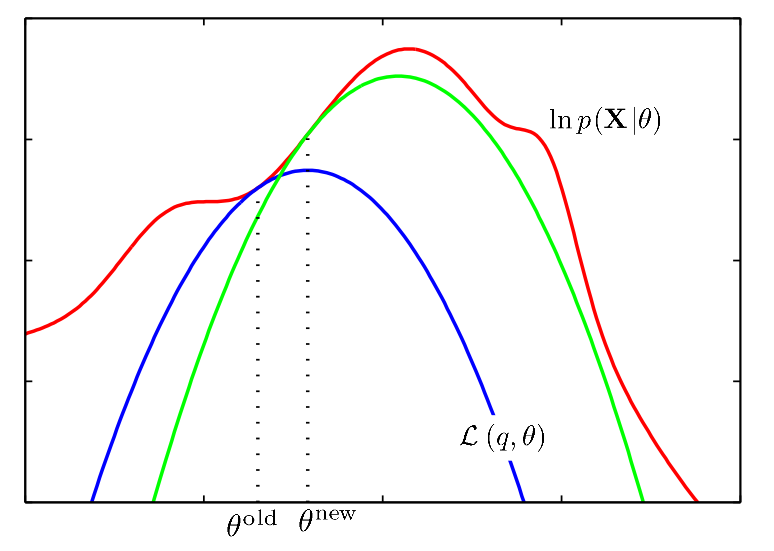
\includegraphics[scale=0.3]{./images/generative/em_update.png}
	\end{center}
	\caption{M-step of EM algorithm}
	\label{fig:em2}
\end{figure}

\section{Alternative View of EM}
The goal of the EM algorithm is to find maximum likelihood (loglikelihood) solutions for models having latent variables.
$$\ln p(X|\theta) = ln\sum_Z p(X,Z|\theta).$$
We are not given the complete data set ${X, Z}$, but only the incomplete data $X$. Our state of knowledge of the values of the latent variables
in $Z$ is given only by the posterior distribution $p(Z|X, \theta)$. Because we cannot use the complete-data log likelihood, we consider instead its expected value under the posterior distribution of the latent variable, which corresponds (as we shall see) to the E step of the EM algorithm.

In the subsequent M step, we maximize this expectation. If the current estimate for the parameters is denoted $\theta_{old}$, then a pair of successive E and M steps gives rise to a revised estimate $\theta^{new}$.

The algorithm is initialized by choosing some starting value for the parameters $\theta_0$. The use of the expectation may seem somewhat arbitrary.

In the E step, we use the current parameter values $\theta^{old}$ to find the posterior distribution of the latent variables given by $p(Z|X, \theta^{old})$. We then use this posterior distribution to find the expectation of the complete-data log likelihood evaluated for some general parameter value $\theta$. This expectation, denoted $Q(\theta, \theta^{old})$, is given by 
$$Q(\theta, \theta^{old}) = \sum_Z p(Z|X, \theta^{old})\ln p(X,Z|\theta).$$
In the M step, we determine the revised parameter estimate $\theta^{new}$ by maximizing this function
$$\theta^{new}=\argmax Q(\theta, \theta^{old}).$$


\begin{algorithm}
The goal is to maximize the likelihood function $p(X|\theta)$ with respect to $\theta$ given a joint distribution $p(X, Z|\theta)$.\\
1. Init $\theta^{old}$\\
2. E-Step: evaluate $p(Z|X, \theta^{old})$ \\
3. M-Step: evaluate $\theta^{new}$ given by 
$$\theta^{new} = \argmax Q(\theta, \theta^{old}),$$
where
$$Q(\theta, \theta^{old}) = \sum_Z p(Z|X, \theta^{old})\ln p(X,Z|\theta).$$
4. Check for convergence of either the log likelihood or the parameter values. If the convergence criterion is not satisfied, then let
$$\theta^{old}\leftarrow \theta^{new}.$$
Return to the step 2. 
\caption{General EM algorithm}
\end{algorithm}



\section{Latent Variable Modeling}

For each object $x_i$, we establish additional latent variable $z_i$ which denotes the index of gaussian from which $i$-th object was generated. Then our model is
$$p(X,Z|\theta) = \prod_{i=1}^{n}p(x_i,z_i|\theta) = \prod_{i=1}^{n}p(x_i|z_i,\theta)p(z_i|\theta) = \prod_{i=1}^{n}\mathcal{N}(x_i|\mu_{z_i},\sigma_{z_i}^2)\pi_{z_i},$$
where $\pi_{j} = p(z_i=j)$ are prior probability of $j$-th gaussian and $\theta = \{\mu_j, \sigma_j, \pi_j\}_{j=1}^K$. If we know both $X$ and $Z$ then we can obtain explicit ML-solution:
$$\theta_{ML} = \argmax_{\theta}p(X,Z|\theta) = \argmax_{\theta}\log p(X,Z|\theta).$$
However, in practice, we don't know $Z$, but only know $X$. Thus, we need to maximize w.r.t. $\theta$ the log of incomplete likelihood
\begin{align}
	\log p(X|\theta) & = \ln \int  p(X, Z|\theta)dZ\\
					 & = \ln\int q(Z|X) \frac{p(X, Z|\theta)}{q(Z|X)}dZ\\
					 & \geq \underbrace{\int q(Z|X) \ln\frac{p(X, Z|\theta)}{q(Z|X)}dZ}_{\textrm{ELBO, } \mathcal{L}(q,\theta)} \quad\textrm{by Jensen's Inequality.}\\
					 &= \int q(Z|X) \ln p(X, Z|\theta) - q(Z|X)\ln q(Z|X)dZ\\
					 &= \int q(Z|X)[\ln p(X|Z,\theta) + \ln p(Z|\theta)]  - q(Z|X)\ln q(Z|X)dZ\\
					 &= \int q(Z|X)\ln p(X|Z,\theta)  - q(Z|X)\ln\frac{q(Z|X)}{p(Z|\theta)}dZ\\
					 &= \mathbb{E}_{q(Z|X)} \ln p(X|Z,\theta)  - KL(q(Z|X)||p(Z|\theta)) 
	% & = \int q(Z)\log \frac{p(X,Z|\theta)}{p(Z|X,\theta)}dZ\\
	% & = \int q(Z)\log \frac{q(Z)p(X,Z|\theta)}{q(Z)p(Z|X,\theta)}dZ\\
	% & = \int q(Z)\log \frac{p(X,Z|\theta)}{q(Z)}dZ+ \int q(Z)\log \frac{q(Z)}{p(Z|X,\theta)}dZ\\
	% & = \underbrace{\int q(Z)\log \frac{p(X,Z|\theta)}{q(Z)}dZ}_{\textrm{ELBO, } \mathcal{L}(q,\theta)}+ \textrm{KL}(q(Z)||\log p(Z|X,\theta))
	\label{eq:elbo}
\end{align}
% Note that $\textrm{KL}( \cdot|| \cdot)\geq 0$, thus $\mathcal{L}(q,\theta) \leq \log p(X|\theta)$. In other words, $\mathcal{L}(q,\theta)$ is a \textbf{lower bound} on $\log p(X|\theta)$.

% Let's see ELBO in a different perspective
% \begin{align*}
% 	\mathcal{L}(q,\theta) &=  \int q(Z)\log \frac{p(X,Z|\theta)}{q(Z)}dZ\\
% 	&= \int q(Z)\Big[\log p(X,Z|\theta)- \log q(Z)\Big]dZ\\
% 	&= \int q(Z)\Big[\log p(Z|X,\theta)+\log p(X|\theta)-\log q(Z)\Big]dZ\\
% 	&= \int q(Z)\log p(X|\theta)dZ+\int q(Z) \log\frac{ p(Z|X,\theta)}{ q(Z)}dZ\\
% 	&= \log p(X|\theta)-\textrm{KL}(q(Z)||p(Z|X,\theta))
% \end{align*}
To maximize the above equation, we need to minimize KL divergence. 

% Also note that $p$ does not depend of $q$, \textbf{so maximizing ELBO is equal to minimizing the KL divergence}. 

% By using ELBO, we are able to maximize the incomplete likelihood. If you see the KL term, it is trying to minimize the divergence between $q(Z)$ and $p(Z)$ through maximizing ELBO.


\subsection{Evidence Lower Bound (ELBO)}
For any choice of inference model $q_{\phi}(z|x)$, we can represent the marginal probability of data (or model evidence) distribution, since the $z$ is not related to $x$, so the integration does not affect $x$. Thus, we can also derive ELBO as follows:
\begin{align*}
	\log p_{\theta}(x) &= \mathbb{E}_{q_{\phi}(z|x)}[\log p_{\theta}(x)]\\
	& = \mathbb{E}_{q_{\phi}(z|x)}\Bigg[\log \frac{p_{\theta}(x,z)}{p_{\theta}(z|x)}\Bigg]\\
	& = \mathbb{E}_{q_{\phi}(z|x)}\Bigg[\log \frac{p_{\theta}(x,z)q_{\phi}(z|x)}{q_{\phi}(z|x) p_{\theta}(z|x)}\Bigg]\\
	& = \underbrace{\mathbb{E}_{q_{\phi}(z|x)}\Bigg[\log \frac{p_{\theta}(x,z)}{q_{\phi}(z|x) }\Bigg]}_{=\mathcal{L}(\phi,\theta)(x)}+\underbrace{ \mathbb{E}_{q_{\phi}(z|x)}\Bigg[\log \frac{q_{\phi}(z|x)}{p_{\theta}(z|x)}\Bigg]}_{=D_{KL}(q_{\phi}(z|x)||p_{\theta}(z|x))}
\end{align*}

To get more intuition about ELBO, we can express ELBO as follows:
\begin{align*}
	\mathcal{L}(\phi,\theta) & = \mathbb{E}_{q_{\phi}(z|x)}\Bigg[\log \frac{p_{\theta}(x,z)}{q_{\phi}(z|x) }\Bigg]\\
	& = \mathbb{E}_{q_{\phi}(z|x)}\Bigg[\log p_{\theta}(x,z)-\log q_{\phi}(z|x)\Bigg]\\
	& = \mathbb{E}_{q_{\phi}(z|x)}\Bigg[\log p_{\theta}(x)+\log p_{\theta}(z|x)-\log q_{\phi}(z|x)\Bigg]\\
	& = \log p_{\theta}(x) - D_{\textrm{KL}}(q_{\phi}(z|x)||p_{\theta}(z|x))\\
	& \leq \log p_{\theta}(x)
\end{align*}

ELBO can be also written as follows:
\begin{align*}
\mathcal{L}(\phi,\theta) & = \mathbb{E}_{q_{\phi}(z|x)}\Bigg[\log \frac{p_{\theta}(x,z)}{q_{\phi}(z|x) }\Bigg]\\
& = \mathbb{E}_{q_{\phi}(z|x)}\Bigg[\log p_{\theta}(x,z)-\log q_{\phi}(z|x)\Bigg]\\
& = \mathbb{E}_{q_{\phi}(z|x)}\Bigg[\log p_{\theta}(z)+\log p_{\theta}(x|z)-\log q_{\phi}(z|x)\Bigg]\\
& = \mathbb{E}_{q_{\phi}(z|x)}[\log p_{\theta}(x|z)] - D_{\textrm{KL}}(q_{\phi}(z|x)||p_{\theta}(z))\\
\end{align*}

We can get a conclusion that maximizing ELBO is equivalent to minimizing the KL divergence through the above equation. Fianlly, the log-likelihood can be rewritten as follows:
\begin{align*}
	\log p_{\theta}(x) = \mathcal{L}(\phi,\theta) + D_{\textrm{KL}}(q_{\phi}(z|x)||p_{\theta}(z|x))
\end{align*}


%\section{Variational Lower Bound}
%Function $g(\xi, x)$ is called variational lower bound for function $f(x)$ iff
%\begin{itemize}
%	\item For all $\xi$ for all $x$ if follows $f(x)\geq g(\xi, x)$
%	\item For any $x_0$ there exists $\xi(x_0)$ such that $f(x_0)=g(\xi(x_0), x_0)$
%\end{itemize} 

\subsection{Expectation Maximization}
We want to maximize ELBO, $\mathcal{L}(q,\theta)$ to minimize KL divergence between $q(Z)$ and $\log p(Z|X,\theta)$.
$$\max_{q,\theta}\mathcal{L}(q,\theta) = \max_{q,\theta}\int q(Z)\log \frac{p(X,Z|\theta)}{q(Z)}dZ.$$
We start from initial point $\theta_0$ and iteratively repeat \Ni E-step and \Nii M-step, iteratively:
\begin{itemize}
	\item E-Step: $\theta_0$ is fixed. 
		$$q(Z) = \argmax_{q}\mathcal{L}(q,\theta) = \argmin_{q}\textrm{KL}(q(Z)|p(Z|X,\theta)) = p(Z|X,\theta_0).$$ 
		\begin{itemize}
			\item This is because, maximizing ELBO is equal to minimizing KL divergence and the minimum $q$ can be achieved when $q$ is equal to $p(Z|X,\theta_0)$.
			\item Now, we just have to evaluate $p(Z|X,\theta_0)$.
		\end{itemize}
	\item M-Step: $q$ is fixed.
		$$\theta_* = \argmax_{\theta}\mathcal{L}(q,\theta) = \argmax_{\theta}\mathbb{E}_{q(Z)}[\log p(X,Z|\theta)]$$
		\begin{itemize}
			\item Can be accomplished by taking derivatives
			\item Set $\theta_0=\theta_*$ and go to the E-Step until convergence
		\end{itemize}
	
\end{itemize}

\subsection{Categorical Latent Variables}
$z_i \in \{1,...,K\}$
$$p(x_i|\theta) = \sum_{k=1}^{K}p(x_i|k,\theta)p(z_i=k|\theta)$$
is simply a finite mixture of distributions. 

E-Step:
$$q(z_i=k) = p(z_i=k|x_i,\theta) = \frac{p(x_k|z_i=k,\theta)p(z_i=k|\theta)}{\sum_{l=1}^{K}p(x_i|z_i=l,\theta)p(z_i=l|\theta)}$$
M-Step:
$$\argmax_{\theta}\mathbb{E}_{q(Z)}[\log p(X,Z|\theta)] = \sum_{i=1}^{n}\mathbb{E}_{q(z_i)}[\log p(x_i,z_i|\theta)] = \sum_{i=1}^{n}\sum_{k=1}^{K}q(z_i=k)\log p(x_i,k|\theta)$$

For GMM, we model $p(x|z)$ as Gaussian.

%\subsection{Continous Latent Variables}
%Continuous latent variables can be regarded as a mixture model of continous distributions. 
%$$p(x_i|\theta) = \int p(z_i|x_i,\theta) dz_i = \int p(x_i|z_i,\theta)p(z_i|\theta) dz_i$$
%E-step can be done in a closed from only in case of conjugate distributions, otherwise the true posterior is intractadble.
%$$q(z_i) = p(z_i|x_i,\theta) = \frac{p(x_k|z_i,\theta)p(z_i|\theta)}{\int p(x_i|z_i,\theta)p(z_i|\theta)dz_i}$$
%
%Typically, continuous latent variables are used for dimension reduction techniques also known as \textbf{representation learning.}

% \part{Deep Generative Models}
\chapter{Explicit Generative Models}
\section{Variational Autoencoder}

Our goal is to find the data distribution $p(X)$. \Cref{fig:dgm} represents a general structure of deep generative model. As you can see, we first sample $z\sim p(z)$ and feed it into a deep neural network $f(z)$ and output $x$.

\begin{figure}[h]
	\begin{center}
		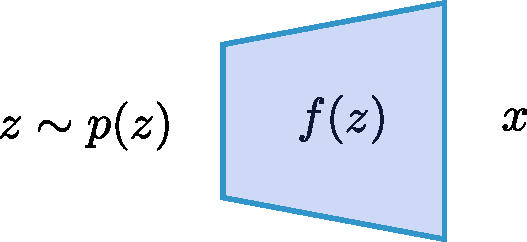
\includegraphics[scale=0.5]{./images/generative/dgm.pdf}
	\end{center}
	\caption{General structure of deep generative models. This model does not infer $z$ from $x$.}
	\label{fig:dgm}
\end{figure}

VAE performs an inference by introducing a probabilistic encoder, called inference network. VAEs are generative model with a latent variable distributed according to some distribution $p(z_i)$. The observed variable is distributed according to a conditional distribution 
$$p_\theta(x_i|z_i)$$
This conditioning means the latent variable values are the one most likely given the observations. We also create a distribution $q_\phi(z_i|x_i)$. We would like to be able to encode our data into the latent variable space. Let's model the distribution.

\begin{itemize}
	\item $p_\theta(x_i|z_i)\sim \mathcal{N}(x_{i}|\mu(z_i), \sigma^2(z_i))$: A probabilistic decoder (or generative network, $\theta$)
	\item $q_\phi(z_i|x_i)$: A probabilistic encoder (or inference network $\phi$). We can choose a family of distributions for our conditional distribution $q$ (\eg standard Gaussian distribution). 
		$$q_\phi(z_i|x_i) = \mathcal{N}(z_i|\mu(x_i, W_1), \sigma^2(x_i, W_2)I),$$
	where $W_1$ and $W_2$ are network weights and collectively denoted as $\phi$. We create a neural network to model the distribution $q$ from our data in a non-linear manner. The outputs of the network are $\mu$ and $\sigma$. 
\end{itemize}

\begin{figure}[h]
	\begin{center}
		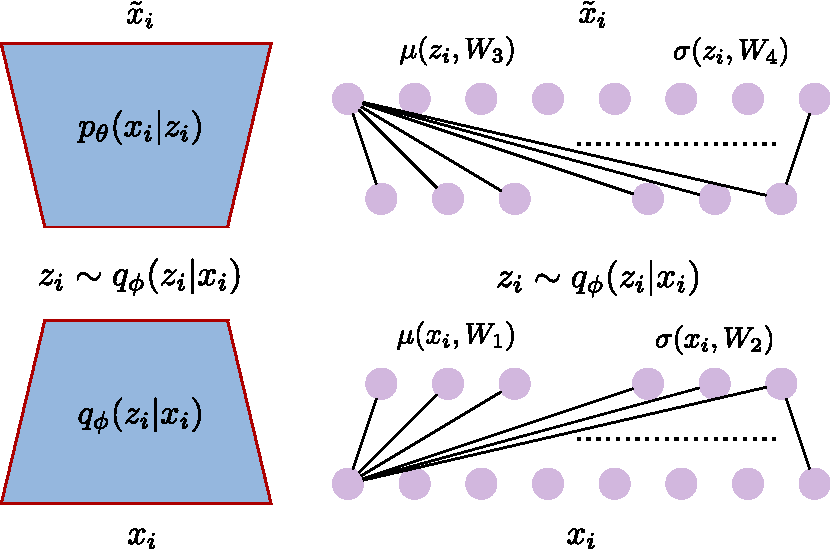
\includegraphics[scale=0.5]{./images/generative/encoder.pdf}
	\end{center}
	\caption{Overview of variational autoencoder.}
	\label{fig:vae}
\end{figure}



\begin{align*}
	p(X,Z|\theta) &=  \prod_{i=1}^{n}\underbrace{p(x_i|z_i,\theta)}_{\textrm{Likelihood, Generator}}\underbrace{p(z_i|\theta)}_{\textrm{Prior on latent variable}}\\
	&= \prod_{i=1}^{n} \mathcal{N}(x_{i}|\underbrace{\mu(z_i), \sigma^2(z_i)}_{\textrm{Non-linear}}) \mathcal{N}(z_i|0, I)
\end{align*}

Subsequently, marginal distributions can be expressed as follows under i.i.d. assumption:
\begin{align*}
	p(X|\theta) &= \prod_{i=1}^{n} p(x_i|\theta) \\
	&= \prod_{i=1}^{n} \int p(x_i, z_j|\theta) dz_j \\
	& = \prod_{i=1}^{n} \int p(x_i|z_i, \theta)p(z_i|\theta)dz_i \\
	& = \prod_{i=1}^{n} \int \mathcal{N}(x_{i}|\mu(z_i), \sigma^2(z_i)) \underbrace{\mathcal{N}(z_i|0, I)}_{\textrm{Mixture weight}} dz_i
\end{align*}

\begin{itemize}
	\item As you can see, the marginal distribution $p(X|\theta)$ becomes a mixture of Gaussian (infinite mixture of Gaussian). 
	\item Even though $p(x|z)$ and $p(z)$ are normal, $p(x)$ is not normal, because it is a mixture distribution.
	\item The non-linearity of Gaussian parameters (modeled by a neural network), conjugacy between the prior and the likelihood does not hold anymore.
%	\item Diagonal covariance matrix does not mean the independence between elements of $x$.
	\item Again, $\mu$ and $\sigma$ is non-linear function of $z$ modeled by some non-linear neural network. The neural network works as a powerful non-linear parameter approximator (based on universal approximation theorem). 
	\item Simple prior is used. Let's consider the data $x$ is an image of $100\times 100$ pixels. Then the covariance matrix has to be $10000\times 10000$. Thus, it is common to set a simple prior such as the standard Gaussian (covariance matrix is diagonal matrix). However, even if we set a simple distribution, with the infinite mixture of Gaussian, we can model any distribution.
	\item VAE uses a global parametric model to predict the local
		variational parameters for each data point (\textbf{amortized inference}). 
%	\item Under the simple standard Gaussian prior assumption, the generator, $p(x_i|z_i,\theta)$, returns factorized Gaussian whose mean and variance are non-linear functions of latent variable modelled by deep neural network parameterized by $\theta$.
%	$$p(x_i|z_i,\theta) = \mathcal{N}(x_{i}|\mu(z_i), \sigma^2(z_i))$$
%	\item VAEs uses a simple prior over latent variables and complicated and powerful generator (neural network).
	\item It allows to convert complicated large-dimensional data distributions into simple lower-dimensional latent variable representations.  
%	\item $Std = e^{\frac{1}{2}\log (Var)}$, thus output is the log var
\end{itemize}

\subsection{VAE Optimization}
We can train VAE using variational inference with the following objective function, ELBO:
$$\mathcal{L}(\phi,\theta) = \mathbbm{E}_{q_{\phi}(z|x)}[\log p_{\theta}(x|z)] - D_{\textrm{KL}}(q_{\phi}(z|x)||p_{\theta}(z))$$
Let's closely look at this objective function:
\begin{itemize}
	\item In $q_{\phi}(z|x)$, $x$ is a given data, so it is not stochatic. How to sample $z$?
	\item $q$ has to be deterministic and differentiable. 
	\item[] $\to$ \textbf{Reparameterization trick}!
		$$\tilde{z}\sim q_\phi(z|x) \to \tilde{z}\sim g_{\phi}(\epsilon, x)$$, where $\epsilon\sim p(\epsilon).$

	\item Estimated by using Monte-Carlo estimation 
		$$\mathbbm{E}_{q_{\phi}(z|x)}[\log p_{\theta}(x|z)]\approx \frac{1}{N}\sum_j \log p_{\theta}(x_i|z_j).$$
\end{itemize}

\subsection{Conditional VAE}
If we have label information about data, then it would provide a better optimization of VAE model. Recall that the following objective function is the objective of the original VAE:
$$\mathcal{L}(\phi,\theta) = \mathbbm{E}_{q_{\phi}(z|x)}[\log p_{\theta}(x|z)] - D_{\textrm{KL}}(q_{\phi}(z|x)||p_{\theta}(z))$$
In conditional VAE, 
$$\mathcal{L}(\phi,\theta) = \mathbbm{E}_{q_{\phi}(z|x, y)}[\log p_{\theta}(x|y, z)] - D_{\textrm{KL}}(q_{\phi}(z|x, y)\ ||\ p_{\theta}(z|y))$$

\begin{align}
	\log p(X|Y) & = \ln\int q(Z|X, Y) \frac{p(X, Z|Y)}{q(Z|X, Y)}dZ\\
					 & \geq \underbrace{\int q(Z|X, Y) \ln\frac{p(X, Z|Y)}{q(Z|X, Y)}dZ}_{\textrm{ELBO, } \mathcal{L}(q,\theta)} \quad\textrm{by Jensen's Inequality.}\\
					 &\dots\\
					 &\dots\\
					 &= \mathbb{E}_{q(Z|X,Y)} [\ln p(X|Z,Y)]  - KL(q(Z|X,Y)||p(Z|Y)) 
	% & = \int q(Z)\log \frac{p(X,Z|\theta)}{p(Z|X,\theta)}dZ\\
	% & = \int q(Z)\log \frac{q(Z)p(X,Z|\theta)}{q(Z)p(Z|X,\theta)}dZ\\
	% & = \int q(Z)\log \frac{p(X,Z|\theta)}{q(Z)}dZ+ \int q(Z)\log \frac{q(Z)}{p(Z|X,\theta)}dZ\\
	% & = \underbrace{\int q(Z)\log \frac{p(X,Z|\theta)}{q(Z)}dZ}_{\textrm{ELBO, } \mathcal{L}(q,\theta)}+ \textrm{KL}(q(Z)||\log p(Z|X,\theta))
\end{align}
Note that not we have a prior $p_{\theta}(z|y)$. However, we have no idea about latent variable $z$, so we simply assume that we cannot impact the $z$ by $y$. Thus, we typically set it as a standard normal distribution. Also, we can simply concatenate the input $X$ with $Y$. 

\subsection{Variational Deep Embedding (VaDE)}
The generative process of VADE $p(x, z, c) = p(x|z)p(z|c)p(c)$:
\begin{itemize}
	\item Choose a cluster $c\sim Cat(\pi)$
	\item Choose a latent vector $z\sim \mathcal{N}(\mu_c, \sigma_c^2I)$
	\item Choose a sample $x$:
		\begin{align*}
			x\sim
			\begin{cases}
				Ber(\mu_x)\quad &\textrm{If }$x$ \textrm{ is binary} \\
				\mathcal{N}(\mu_x, \sigma_x^2I) \quad &\textrm{else}
			\end{cases}
		\end{align*}
\end{itemize}
ELBO of VaDE:
\begin{align}
	\log p(X) & = \ln\int \sum_c p(X,Z,C) dz \\
					 & \geq \underbrace{\int q(Z,C|X) \ln\frac{p(X, Z, C)}{q(Z,C|X)}dZ}_{\textrm{ELBO}} 
\end{align}
The ELBO can be decomposed as follows:
\begin{align*}
\mathcal{L}_{ELBO} &= \mathbb{E}_q(z,c|x)\bigg[\ln\frac{p(x,z,c)}{q(z,c|x)}\bigg]\\
				   &= \mathbb{E}_q(z,c|x)[\ln p(x,z,c) - \ln q(z,c|x)]\\
				   &= \mathbb{E}_q(z,c|x)[\ln p(x|z) + \ln p(z|c)+ \ln p(c)-\ln q(z|x)-\ln q(c|x)]
\end{align*}
By using two factorizations:
\begin{itemize}
	\item $p(x, z, c) = p(x|z)p(z|c)p(c)$
	\item $q(z,c|x) \approx q(z|x)q(c|x)$ (Mean-field assumption)
		\begin{itemize}
			\item $q(z|x)\sim \mathcal{N}$: encoder, estimate mean and variance.
			\item $q(c|x)$: assignment probability of Gaussian mixture model
		\end{itemize}
\end{itemize}

\subsection{Importance Weighted VAE}


% \begin{itemize}
% 	\item 
% 		$$\mathbbm{E}_{q_{\phi}(z|x)}[\log p_{\theta}(x|z)]\approx \frac{1}{N}\sum_j \log p_{\theta}(x_i|z_j).$$
% 	\item The second term can be solve analytically for some distributions like Gaussian.
% 	\item For training, we need to use a reparameterization trick. 
% \end{itemize}




%\footnotetext[1]{Uncorrelated relationship does not imply the independence (independence makes covariance to be diagonal). If two variables are uncorrelated, $Cov(x_i,x_j)=0 $, there is no linear relationship between them.}
%\footnotetext[2]{In practice, simple prior could be a problem.}

\chapter{Implicit Generative Models}
\section{Generative Adversarial Networks}
\label{sec:gan}
\begin{itemize}
	\item Generator's distribution: $p_{g}$
	\item Prior on input noise: $p_{z}(z)$
	\item Mapping to data space: $z\rightarrow x$ through $G(z;\theta_{g})$
	\item[] a differentiable multilayer perceptron with parameter $\theta_{g}$
	\item $D(x;\theta_{d})$: a differentiable multilayer perceptron with parameter $\theta_{d}$. It outputs a single scalar 
	\item $D(x)$: probability that $x$ (real) came from the data rather than $p_g$ (fake)
\end{itemize}

\begin{figure}[h]
	\begin{center}
		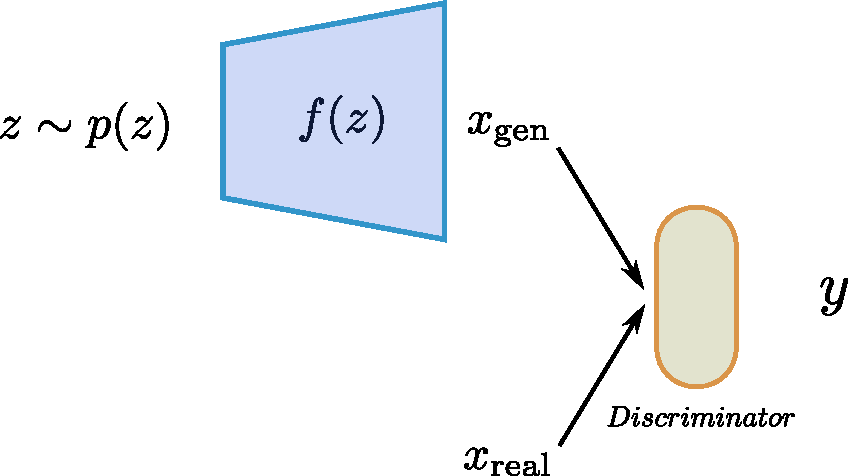
\includegraphics[scale=0.5]{./images/generative/gan/gan_model.pdf}
	\end{center}
	\caption{GAN structure}
	\label{fig:gan}
\end{figure}

\subsection{Discriminator}
The discriminator's goal is to maximize the following equation given $G$
\begin{equation*}
\mathbbm{E}_{x \sim p_{data}(x)}\log(D(x))+\mathbbm{E}_{z \sim p_{z}(z)}\log(1-D(G(z)))
\end{equation*}
The optimal discriminator given $G$ can be denoted as $D^*_{G}$. To get the optimal discriminator, define a value function
\begin{equation*}
V(G,D):= \mathbbm{E}_{x \sim p_{data}(x)}\log(D(x))+\mathbbm{E}_{z \sim p_z(z)}\log(1-D(G(z))).
\end{equation*}
Then, $D_G^* = \text{argmax}_D V(G,D)$

However, the generator $G$ wants to minimize the value function given $D=D^*_G$. 
\begin{equation*}
G^* = \text{argmin}_G V(G,D_G^*).
\end{equation*}

\begin{equation*}
\min_{G}\max_{D}V(D,G) =  \mathbbm{E}_{x\sim p_{data}(x)}[\textrm{log}D(x)]+\mathbbm{E}_{z\sim p_{z}(z)}[\textrm{log}(1-D(G(z)))]
\end{equation*}
\begin{itemize}
	\item $\min_{G} \rightarrow$ try to generate fake data that is similar to real data
	\item $\max_{D} \rightarrow$ try to assign correct label \footnotemark
\end{itemize}

At this point, we must show that this optimization problem has a unique solution $G^*$ and that this solution satisfies $p_G=p_{data}$.

\footnotetext{The above equation is trained separately at the same time, don't get confused}

One big idea from the GAN paper–, which is different from other approaches is that $G$ \textbf{need not be invertible}. Many pieces of notes online miss this fact when they try to replicate the proof and incorrectly use the change of variables formula from calculus (which would depend on $G$ being invertible). Rather, the whole proof relies on this equality:
\begin{equation*}
	\mathbbm{E}_{z \sim p_{z}(z)}\log(1-D(G(z))) = \mathbbm{E}_{x \sim p_{G}(x)}\log(1-D(x)) .
\end{equation*}

With the above equality, 
\begin{align*}
	&\mathbbm{E}_{x \sim p_{data}(x)}\log(D(x))+\mathbbm{E}_{z \sim p_z(z)}\log(1-D(G(z)))\\
	&=\int_{x} p_{data}(x)\log D(x) \, \mathrm{d}x + \int_{z} p(z)\log ( 1- D(G(z))) \, \mathrm{d}z\\ 
	&= \int_{x} p_{data}(x)\log D(x) + p_G(x) \log ( 1- D(x)) \, \mathrm{d}x
\end{align*}

Additionally, we will use the following property:
\begin{align*}
	f(y)= a \log y + b \log(1-y).
\end{align*}
To find a critical point,
$$f^\prime(y) = 0 \Rightarrow \frac{a}{y} - \frac{b}{1-y} = 0 \Rightarrow y = \frac{a}{a+b}$$
If $a+b\neq0$, do the second derivative test:
$$f^{\prime\prime}\big ( \frac{a}{a+b} \big) = - \frac{a}{(\frac{a}{a+b})^2} - \frac{b}{(1-\frac{a}{a+b})^2} < 0
$$
If $a,b\in (0,1)$, $\frac{a}{a+b}$ is a maximum.

By rewriting the equation,
\begin{align*}
V(G,D) &= \int_{x} p_{data}(x)\log D(x) + p_G(x) \log ( 1- D(x)) \, \mathrm{d}x \\
& \leq \int_x \max_y {p_{data}(x)\log y + p_G(x) \log ( 1- y)}\, \mathrm{d}x 
\end{align*}
Thus, if $D(x) = \frac{p_{data}}{p_{data}+p_G}$, then we can achieve the maximum $V(G,D)$. 

\subsection{Generator}
If we achieve the optimal $G$ (i.e., $p_G = p_{data}$), then $D$ would be completely confused and $D^*_G(x) = \frac{p_{data}}{p_{data}+p_G}=\frac{1}{2}$ (it means that $D$ cannot make a clear decision.).

The global minimum of the virtual training criterion $C(G)=\max_DV(G,D)$ is acheived if and only if $p_{G}=p_{data}$. Let's plug $D^*_G(x)$ into the criterion then, 
\begin{equation*}
	C(G) = \int_{x} p_{data}(x)\log \big (\frac{p_{data}(x)}{p_{G}(x)+p_{data}(x)} \big )  + p_G(x) \log\big ( \frac{p_{G}(x)}{p_{G}(x)+p_{data}(x)}\big ) \, \mathrm{d}x. 
\end{equation*}
To get the minimum $C(G)$, we can use the Jansen-Shannon divergence:

\begin{align*}
	D_{JS}(p_{data}||p_{G}) & = \frac{1}{2}\Bigg[D_{KL}\Big(p_{data}\Big|\Big|\frac{p_{data}+p_{G}}{2}\Big)+D_{KL}\Big(p_{G}\Big|\Big|\frac{p_{data}+p_{G}}{2}\Big)\Bigg]\\
	& = \frac{1}{2}\Bigg[\Bigg(\int_x p_{data}(x)\textrm{log}\Bigg(\frac{2p_{data}(x)}{p_{data}(x)+p_{G}(x)}\Bigg)dx\Bigg)+\Bigg(\int_x p_{G}(x)\textrm{log}\Bigg(\frac{2p_{G}(x)}{p_{data}(x)+p_{G}(x)}\Bigg)dx\Bigg)\Bigg]\\
	& = \frac{1}{2}\Bigg[\Bigg(\int_x p_{data}(x)\textrm{log}2+p_{data}(x)\textrm{log}\Bigg(\frac{p_{data}(x)}{p_{data}(x)+p_{G}(x)}\Bigg)dx\Bigg)+\\
	&\hspace{1cm}\Bigg(\int_x p_{G}(x)\textrm{log}2+p_{G}(x)\textrm{log}\Bigg(\frac{p_{G}(x)}{p_{data}(x)+p_{G}(x)}\Bigg)dx\Bigg)\Bigg]\\
	& = \frac{1}{2}\Bigg[\Bigg(\textrm{log}2+\int_x p_{data}(x)\textrm{log}\Bigg(\frac{2p_{data}(x)}{p_{data}(x)+p_{G}(x)}\Bigg)dx\Bigg)+\\
	& \hspace{1cm}\Bigg(\textrm{log}2+\int_x p_{G}(x)\textrm{log}\Bigg(\frac{2p_{G}(x)}{p_{data}(x)+p_{G}(x)}\Bigg)dx\Bigg)\Bigg]\\
	& = \frac{1}{2}(\textrm{log}4+C(G))
\end{align*}

Thus,
$$C(G) = -\textrm{log}4 + 2D_{JS}(p_{data}||p_{G})$$

Since the Jensen-Shannon divergence between two distributions is always non-negative and zero only when they are equal, we have shown that $C^* = -\textrm{log}(4)$ is the global minimum of $C(G)$ and that the only solution is $p_G=p_{data}$, i.e., the generative model perfectly replicating the data generating process.

\begin{figure}[h]
	\centering
	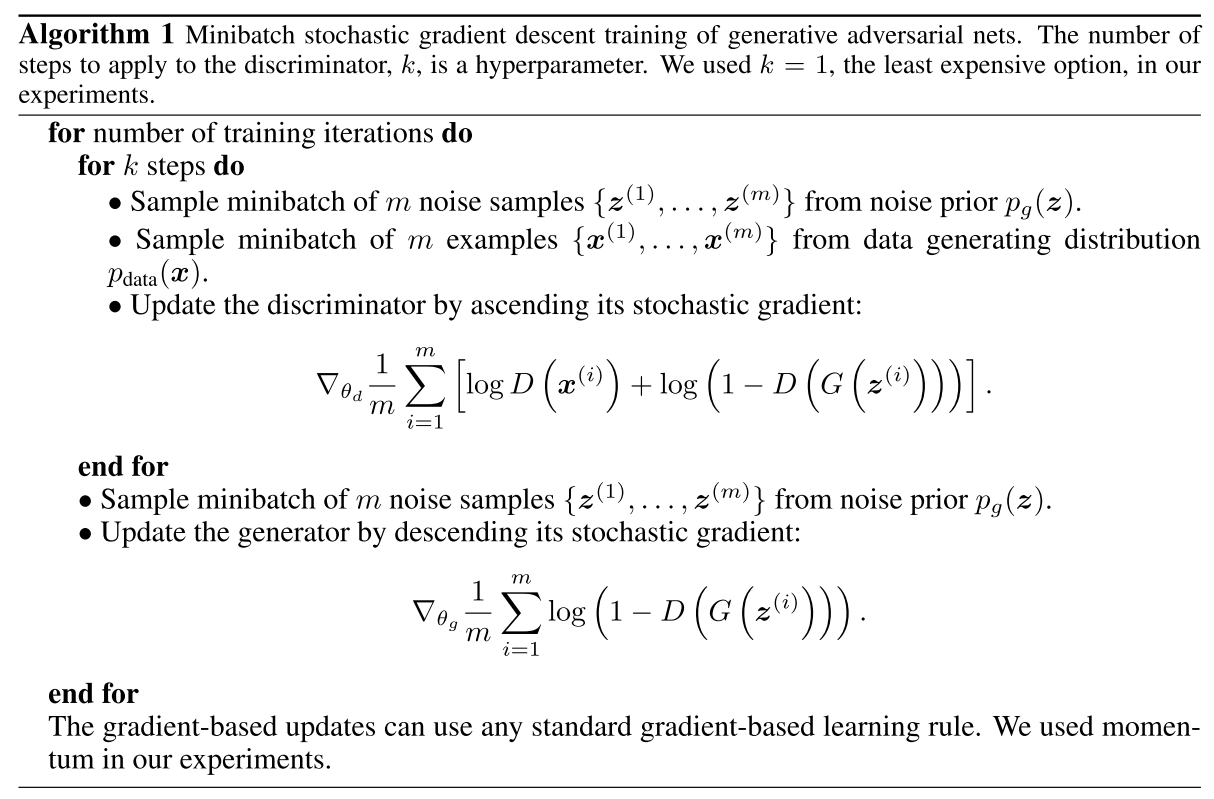
\includegraphics[scale=0.3]{./images/generative/gan/gan_algorithm.png}
	\caption{Training GAN}
	\label{fig:algorithm}
\end{figure}

\section{Some notes}
What would be the optimal discriminator that separates the two different distributions $p(x)$ and $q(x)$? It turns out that it is
$$f(x) = \frac{q(x)}{p(x)+q(x)}$$
Actually, there are many choices for classifiers e.g., KL-divergence

\begin{enumerate}
	\item What do we need to learn a classifier?
	\begin{itemize}
		\item Only samples from $p(x)$ and $q(x)$
	\end{itemize}
	\item How do we parameterize $q(x)$?
	\begin{itemize}
		\item Parametric density function (Gaussian)
		\item Define implicitly (GANs approach): define mapping from one (noise) to another (data or image)
	\end{itemize}
\end{enumerate}

The orignal GAN does not learn the data distributions. 





\section{Wasserstein Generative Adversarial Networks}
\subsection{KL Divergence}
Definition:
$$D_\textrm{KL}(q(x)||p(x)) = \int q(x)\log \frac{q(x)}{p(x)}dx$$
\begin{itemize}
	\item Forward KL: 
	\begin{itemize}
		\item If $q(z)\rightarrow 0, \textrm{Forward KL}\rightarrow \infty$ 
		\item Zero avoiding for $q(z)$ 
	\end{itemize}
	\item Reverse KL:
	\begin{itemize}
		\item If $p(z)\rightarrow 0, \textrm{Reverse KL}\rightarrow \infty$ 
		\item Zero forcing: $q(z)\rightarrow 0$ 
	\end{itemize}
\end{itemize}

Typically, $p(x)$ and $q(x)$ are far apart at the initial state. 

\begin{figure}[h]
	\begin{center}
		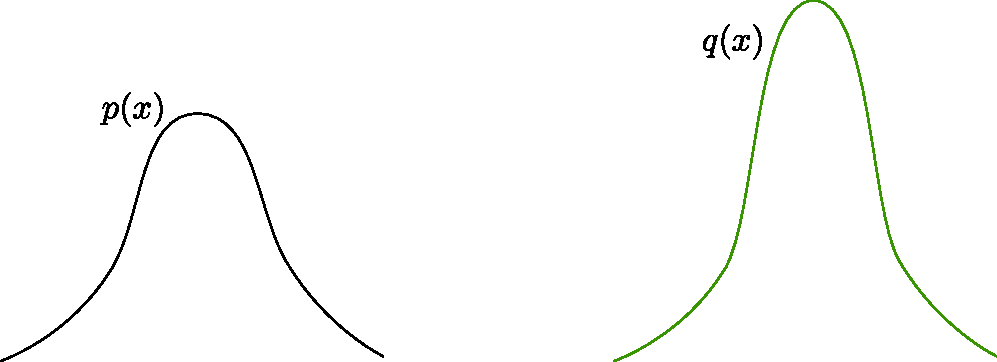
\includegraphics[scale=0.5]{./images/generative/gan/twodist.pdf}
	\end{center}
	\caption{Two distributions: $p(x)$ and $q(x)$}
	\label{fig:}
\end{figure}

Thus, both the forward KL and the reverse KL suffers an unstability issue. Specifically, in each case, if the denominator goes to zero, then the divergence goes to infinity. 

\subsection{Jensen-Shannon Divergence}

Definition:
$$D_{JS}(p_{data}||p_{G}) = \frac{1}{2}\Bigg[D_{KL}\Big(p_{data}\Big|\Big|\frac{p_{data}+p_{G}}{2}\Big)+D_{KL}\Big(p_{G}\Big|\Big|\frac{p_{data}+p_{G}}{2}\Big)\Bigg]$$

The KL divergence's issue can be alleviated by JS-divergence. Consider a simple example in Fig. \ref{fig:wassersteinexample}6
\begin{align*}
	\forall (x, y) \in P, x = 0 \text{ and } y \sim U(0, 1)\\
	\forall (x, y) \in Q, x = \theta, 0 \leq \theta \leq 1 \text{ and } y \sim U(0, 1)
\end{align*}

\begin{figure}[h]
	\begin{center}
		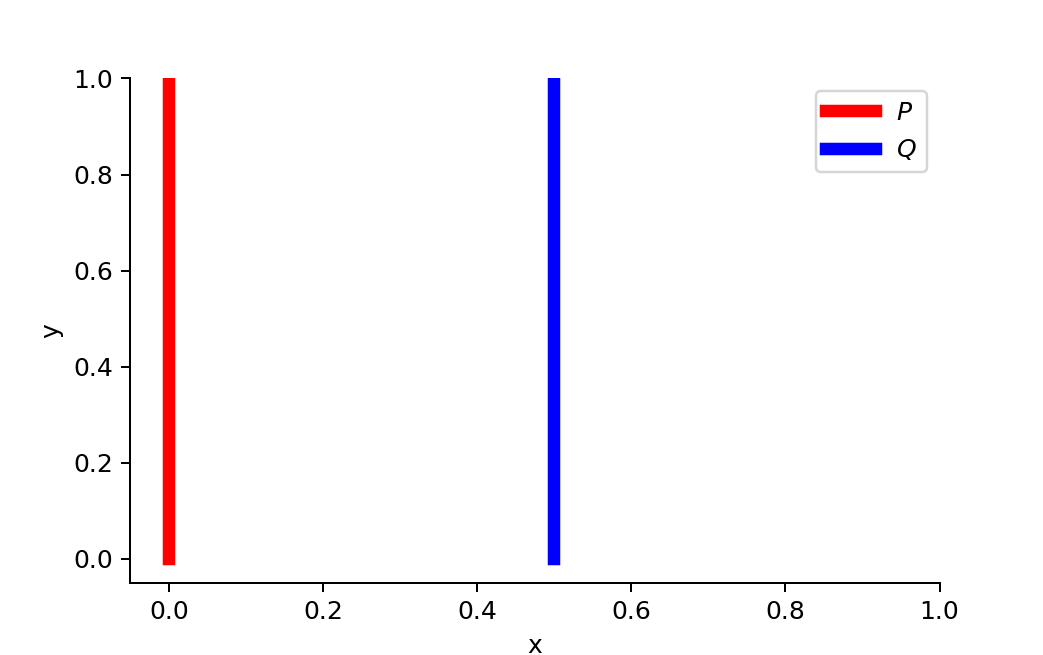
\includegraphics[scale=0.25]{./images/generative/gan/wassersteinexample.png}
	\end{center}
	\caption{Two distributions: $p(x)$ and $q(x)$}
	\label{fig:wassersteinexample}
\end{figure}

\begin{align*}
	D_\textrm{KL}(q(x)||p(x)) &= \infty\\
	D_\textrm{KL}(p(x)||q(x)) &= \infty\\
	D_{JS}(p_{data}||p_{G}) &= \frac{1}{2}\Bigg[D_{KL}\Big(p_{data}\Big|\Big|\frac{p_{data}+p_{G}}{2}\Big)+D_{KL}\Big(p_{G}\Big|\Big|\frac{p_{data}+p_{G}}{2}\Big)\Bigg]\\
	& = \frac{1}{2}\Bigg[D_{KL}\Big(p_{data}\Big|\Big|\frac{p_{data}}{2}\Big)++D_{KL}\Big(p_{G}\Big|\Big|\frac{p_{G}}{2}\Big)\Bigg]\\
	& = \frac{1}{2}[\log 2 + \log 2] = \log 2\\
	W(p,q) & = |\theta|
\end{align*}
Therefore, Jensen-Shannon divergence is more stabler than KL divergece. This is one of the reasons why GAN, which uses JS divergence works better than VAE, which uses KL divergence. 

However, JS divergence also has some problem. If the value is close to $\frac{1}{2}\log 2$, then the gradient will be very small or close to zero, because the divergence is close to constant. It means that a training speed is very slow. Thus, we need a better metric. 

\subsection{Wasserstein Distance}
Wasserstein Distance is a measure of the distance between two probability distributions. It is also called Earth Mover’s distance, short for EM distance, because informally it can be interpreted as the minimum energy cost of moving and transforming a pile of dirt in the shape of one probability distribution to the shape of the other distribution.
\begin{equation*}
	W(p_r, p_g) = \inf_{\gamma \sim \Pi(p_r, p_g)} \mathbbm{E}_{(x, y) \sim \gamma}[\| x-y \|]
\end{equation*}

\begin{itemize}
	\item $\Pi$: is the transportation plan and the set of all possible joint probability distributions between $p_r$ and $p_g$. One joint distribution $\gamma \sim \Pi(p_r, p_g)$ describes one transport plan.\
	\item $\mathbbm{E}_{x, y \sim \gamma} \| x-y \| = \sum_{x, y} \gamma(x, y) \| x-y \|$
	\item Finally, we take the minimum one among the costs of all dirt moving solutions as the EM distance (by infimum). 
\end{itemize}

\section{WGAN}
However, consider all possible joint distribution is intractable, so dual solution can be used. 

$$W(p_r, p_g) = \frac{1}{K} \sup_{\| f \|_L \leq K} \mathbbm{E}_{x \sim p_r}[f(x)] - \mathbbm{E}_{x \sim p_g}[f(x)]$$

So to calculate the Wasserstein distance, we just need to find a 1-Lipschitz function. To enforce the constraint, WGAN applies a very simple clipping to restrict the maximum weight value in $f$, i.e. the weights of the discriminator

Suppose this function $f$ comes from a family of $K$-Lipschitz continuous functions, $\{f_w\}_{w\in W}$, parameterized by $w$. In the modified Wasserstein-GAN, the ``discriminator'' model is used to learn $w$ to find a good $f_w$ and the loss function is configured as measuring the Wasserstein distance between $p_r$ and $p_g$.

$$L(p_r, p_g) = W(p_r, p_g) = \max_{w \in W} \mathbbm{E}_{x \sim p_r}[f_w(x)] - \mathbbm{E}_{z \sim p_r(z)}[f_w(g_\theta(z))]$$

There are two ways to satisfy the Lipschitz continuity:
\begin{itemize}
	\item Weight clipping
	\item Gradient Penalty
\end{itemize}

\subsection{Lipschitz continuity}
The function $f$ in the new form of Wasserstein metric is demanded to satisfy $\| f \|_L \leq K$, meaning it should be $K$-Lipschitz continuous. \citep{Lil2017}

A real-valued function $f: \mathbbm{R} \rightarrow \mathbbm{R}$ is called $K$-Lipschitz continuous if there exists a real constant $K\geq 0$ such that, for all $x_1, x_2 \in \mathbbm{R}$
$$\lvert f(x_1) - f(x_2) \rvert \leq K \lvert x_1 - x_2 \rvert$$
Here $K$ is known as a Lipschitz constant for function $f(\cdot)$. Functions that are everywhere continuously differentiable is Lipschitz continuous, because the derivative, estimated as $\frac{\lvert f(x_1) - f(x_2) \rvert}{\lvert x_1 - x_2 \rvert}$, has bounds. However, a Lipschitz continuous function may not be everywhere differentiable, such as $f(x) = \lvert x \rvert$

\begin{figure}[h]
	\begin{center}
		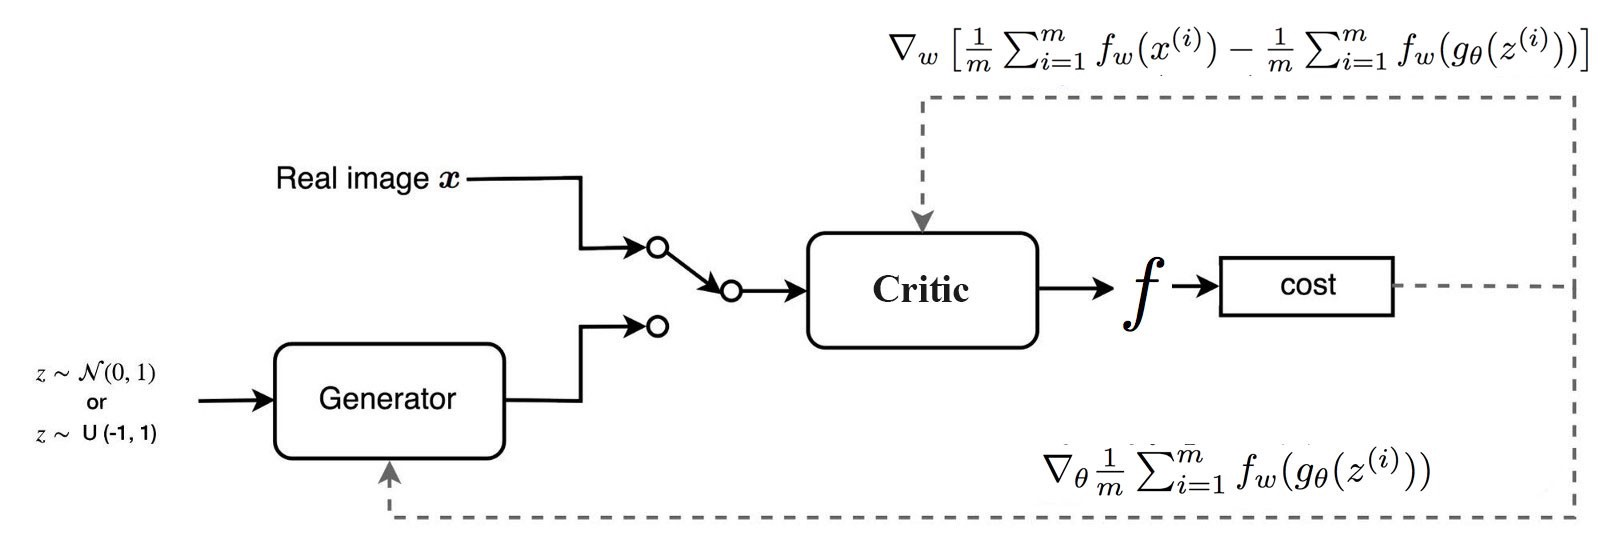
\includegraphics[scale=0.25]{./images/generative/gan/wgan.jpeg}
	\end{center}
	\caption{WGAN}
	\label{fig:wgan}
\end{figure}

\begin{figure}[h]
	\begin{center}
		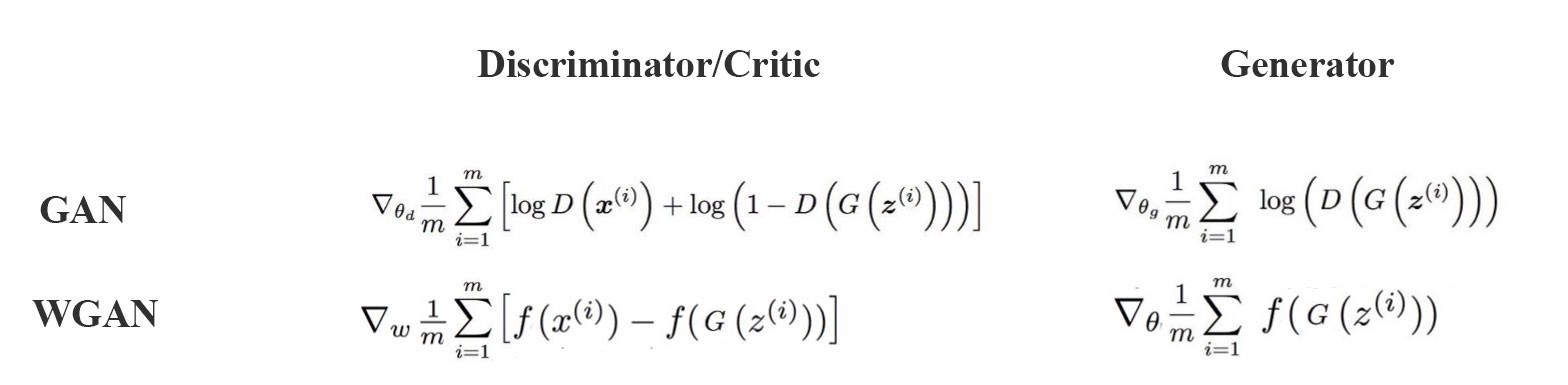
\includegraphics[scale=0.2]{./images/generative/gan/wgan_2.jpeg}
	\end{center}
	\caption{WGAN}
\end{figure}

\section{InfoGAN: Interpretable Representation Learning by Information Maximizing Generative Adversarial Nets}
\label{sec:q}

\subsection{Joint Entropy}
\begin{align*}
H(X,Y) = \mathbb{E}_{X,Y}[-\log p(x,y)] = -\sum_{x,y}p(x,y)\log p(x,y)
\end{align*}
\subsection{Conditional Entropy}
\begin{align*}
H(X|Y) &= \mathbb{E}_{Y}[H(X,Y)] \\
&= -\sum_{y\sim p_Y(y)}p(y)\sum_{x\sim p_X(x)}p(x|y)\log p(x|y)\\
& = -\sum_{y\sim p_Y(y)}\sum_{x\sim p_X(x)}p(y)p(x|y)\log p(x|y)\\
& = -\sum_{y\sim p_Y(y)}\sum_{x\sim p_X(x)}p(x,y)\log p(x|y) = -\mathbb{E}_{x,y}[\log p(x|y)]\\
& = -\sum_{y\sim p_Y(y)}\sum_{x\sim p_X(x)}p(x,y)\log \frac{p(x,y)}{p(y)}\\
& = -\sum_{y\sim p_Y(y)}\sum_{x\sim p_X(x)}p(x,y)\log p(x,y) + \sum_{y\sim p_Y(y)}\sum_{x\sim p_X(x)}p(x,y)\log p(y)\\
& = H(X,Y) - H(Y)
\end{align*}
\subsection{Variational Mutual Information Maximization}
\begin{align*}
I(c;G(z,c)) &= H(c) - H(c|G(z,c))\\
& = H(c) + \int\int p(c=c',x=G(z,c))\log p(c=c'|x=G(z,c)) dc' dz\\
& = H(c) + \mathbb{E}_{x\sim G(z,c),c'\sim p(c|x)}[\log p(c'|x)]\\
& = H(c) + \mathbb{E}_{x\sim G(z,c)}\mathbb{E}_{c'\sim p(c|x)}[\log p(c'|x)]\\
& = H(c) + \mathbb{E}_{x\sim G(z,c)}\mathbb{E}_{c'\sim p(c|x)}\Bigg[\log \frac{p(c'|x)Q(c'|x)}{Q(c'|x)}\Bigg]\\
& = H(c) + \mathbb{E}_{x\sim G(z,c)}\mathbb{E}_{c'\sim p(c|x)}\Bigg[\log \frac{p(c'|x)}{Q(c'|x)}\Bigg] + \mathbb{E}_{x\sim G(z,c)}\mathbb{E}_{c'\sim p(c|x)}\Big[\log Q(c'|x)\Big]\\
& = H(c) + \mathbb{E}_{x\sim G(z,c)}\Bigg[D_{KL}(p(c'|x)||Q(c'|x))\Bigg] + \mathbb{E}_{x\sim G(z,c)}\mathbb{E}_{c'\sim p(c|x)}\Big[\log Q(c'|x)\Big]\\
& \geq H(c) + \mathbb{E}_{x\sim G(z,c)}\mathbb{E}_{c'\sim p(c|x)}\Big[\log Q(c'|x)\Big] \footnotemark
\end{align*}

Thus we get a lower bound for the mutual information as follows:

$$I(c;G(z,c)) \geq H(c) + \mathbb{E}_{x\sim G(z,c)}\mathbb{E}_{c'\sim p(c|x)}\Big[\log Q(c'|x)\Big]$$

However, we still have a problem. We need to sample $c$ from $p(c|x)$. Thus, we need to replace it with a known distribution. Firstly, with the reasoning that $x\sim G(z,c)$ means sample $c$ from $p(c)$ then sample $x$ from $G(z,c)$. So we can express $\mathbb{E}_{x\sim G(z,c)}$ with $\mathbb{E}_{c\sim p(c)}\mathbb{E}_{x\sim G(z,c)}$. and by the Lemma \ref{lemma:1}, 
\begin{align*}
I(c;G(z,c)) &\geq H(c) + \mathbb{E}_{x\sim G(z,c)}\mathbb{E}_{c'\sim p(c|x)}\Big[\log Q(c'|x)\Big]\\
&= H(c) + \mathbb{E}_{c\sim p(c)}\mathbb{E}_{x\sim G(z,c)}\mathbb{E}_{c'\sim p(c|x)}\Big[\log Q(c'|x)\Big]\\
& = H(c) + \mathbb{E}_{c\sim p(c)}\mathbb{E}_{x\sim G(z,c)}\Big[\log Q(c'|x)\Big] \footnotemark
\end{align*}

Thus, we can directly sample $c$ from the known distribution instead of $p(c|x)$.

\begin{lemma}
	For random variables $X, Y$ and function $f(x, y)$ under suitable regularity conditions:
	$$\mathbb{E}_{x\sim X, y\sim Y|x}[f(x,y)] = \mathbb{E}_{x\sim X, y\sim Y|x, x'\sim X|y}[f(x',y)]$$
	\begin{proof}
		\begin{align*}
		\mathbb{E}_{x\sim X, y\sim Y|x}[f(x,y)] &=\int_x P(x)\int_y P(y|x)f(x,y)dydx\\
		& = \int_x\int_yP(x,y)f(x,y)dydx\\
		& = \int_{x'}\int_yP(x',y)f(x',y)dydx'\\
		& = \int_{x'}\int_y P(y)P(x'|y)f(x',y)dydx'\\
		& = \int_{x'}\int_y\int_{x} P(x,y)P(x'|y)f(x',y)dxdydx'\\
		& = \int_{x}P(x)\int_y P(x|y) \int_{x'} P(x'|y)f(x',y)dxdydx'\\
		& = \mathbb{E}_{x\sim X, y\sim Y|x, x'\sim X|y}[f(x',y)]
		\end{align*}
	\end{proof}
	\label{lemma:1}
\end{lemma} 


% \chapter{Introduction}
\section{Introduction}
The HMM is based on the Markov chain assumption. A Markov chain is a model
that tells us something about the probabilities of sequences of random variables,
states, each of which can take on values from some set. These sets can be words, or
tags, or symbols representing anything, like the weather.

There are two important assumptions:
\begin{itemize}
	\item Markov assumption
	\item Output independence: $p(x_i|z_1,\dots,z_i,\dots,z_T,x_1,\dots,x_i,\dots,x_T) = p(x_i|z_i)$
\end{itemize}

\subsection{Conditional Independence}
If two events $A$ and $B$ are \textbf{conditionally independent} given an event $C$ then,
\begin{itemize}
	\item $P(A\cap B|C) = P(A|C)P(B|C)$. 
	\item $P(A|B,C) = P(A|C)$
\end{itemize}

\subsection{Notation}

\begin{itemize}
	\item $X = (x_i, x_2,\dots, x_T)$
	% \item $x_i\in\{c_1,...,c_m\}$
	\item Initial state probabilities: $p(z_1) \sim \textrm{Multinomial}(\pi_1,...,\pi_k)$, need to learn $\pi$
	\item Transition probability:
	$$p(z_t|z_{t-1}=i)\sim \textrm{Multinomial}(a_{i,1},...,a_{i,k})$$
	, where $a_{i,j} = p(z_t=j|z_{t-1}=i)$ and $i$ and $j$ denote clusters or states, respectively.
	\item Emission probability:
	$$p(x_t|z_{t}=i)\sim \textrm{Multinomial}(b_{i,1},...,b_{i,m})$$
	, where $b_{i,j} = p(x_t=j|z_{t}=i)$
\end{itemize}


\section{Bayesian Network}
\subsection{Bayes Ball}

\begin{figure}[h!]
	\centering
	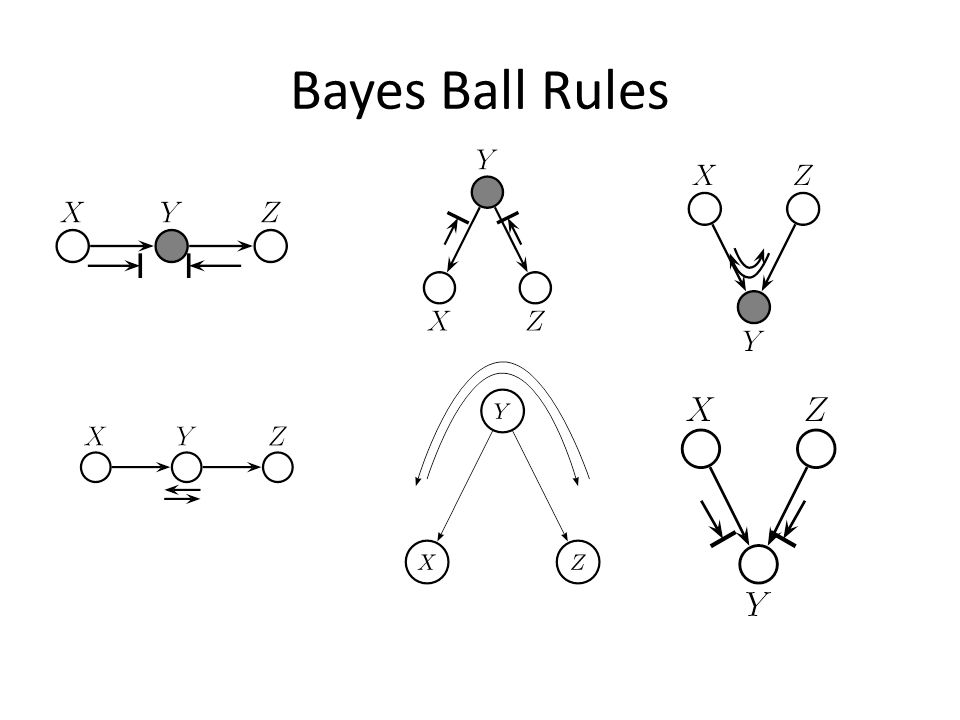
\includegraphics[scale=0.3]{./images/hmm/bayes.jpg}
	\caption{Bayes ball}
	\label{fig:bayes}
\end{figure}

\begin{itemize}
	\item Cascading: $P(Z|Y,X) = P(Z|Y)$. The information of $Y$ decouples $X$ and $Z$.
	\item Common parent: $P(X,Z|Y) = P(X|Y)P(Z|Y)$. The information of $Y$ decouples $X$ and $Z$.
	\item V-Structure (common child): Unlike the above two cases, the information of $Y$ couples $X$ and $Z$.
		$$P(X,Y,Z) = P(X)P(Y)P(Y|X,Z).$$
\end{itemize}

\subsection{Potential Function}
Potential function is a function which is not a probability function, but it can become a probability function by normalizing it. 
$$P(A,B,C,D) = P(A|B)P(B|C)P(C|D)P(D)$$

\begin{figure}[h]
	\centering
	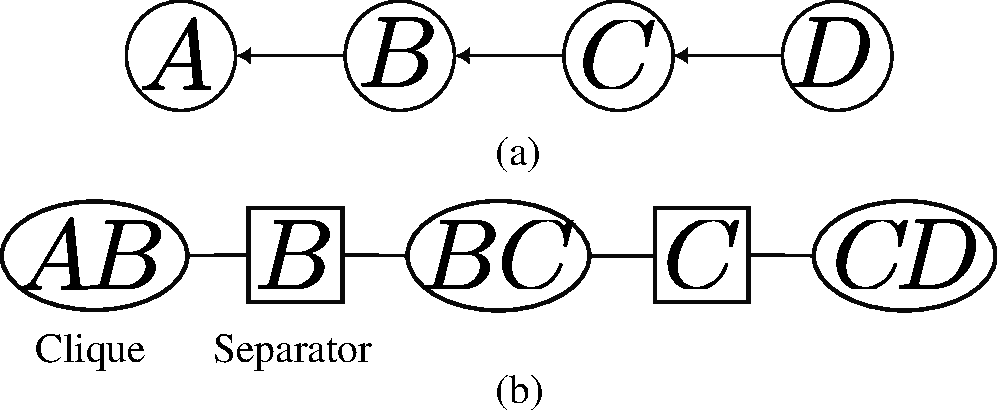
\includegraphics[scale=0.5]{./images/hmm/cascade.pdf}
\end{figure}

\begin{itemize}
	\item Cliques: $\Psi(a,b), \Psi(b,c), \Psi(c,d)$
	\item Separators $\phi(b), \phi(c)$
\end{itemize}
Given a clique tree with cliques and separators, the joint probability distribution is defined as follows:
% By using potential functions, we can express the joint probability as
\begin{align*}
	P(A,B,C,D) &= P(U) = \frac{\prod_N \Psi(N)}{\prod_L\phi(L)}= \frac{ \Psi(a,b)\Psi(b,c)\Psi(c,d)}{\phi(b)\phi(c)}\\
\end{align*}
An effect of an observation propagates through the clique graph $\to$ \textbf{Belief propagation}. How to propagate the belief? \textbf{Absorption rule}!

Let's say we have some new observations about $A$, then it affects the clique $\Psi(a,b)$. The updated clique is now $\Psi^*(a,b)$. Similarly, $\phi^*(b) = \sum_A\Psi^*(a,b)$. Subsequently, $\Psi^*(b,c) = \Psi^(b,c)\frac{\phi^*(b)}{\phi(b)}$.



\chapter{Hidden Markov Model}
\begin{figure}[h]
	\begin{center}
		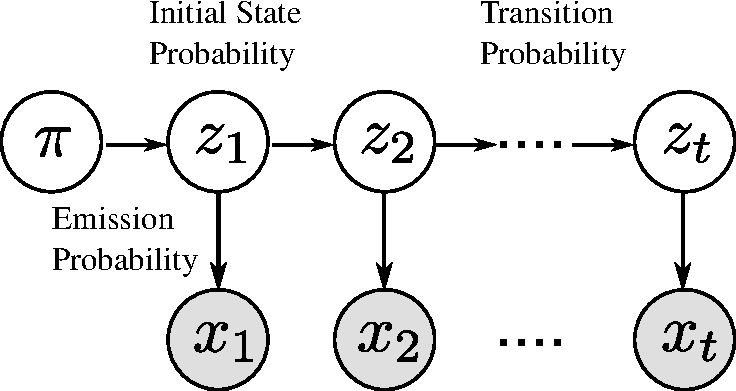
\includegraphics[scale=0.7]{./images/hmm/hmm_figure.pdf}
	\end{center}
	\caption{HMM Structure}
	\label{fig:HMM}
\end{figure}

The observation can be discrete or continuous. If the latent factors are continuous, then HMM is often referred as \textbf{Kalman filter}. 

\begin{itemize}
	\item Initial state probability: $P(z_1)\sim \textrm{Mult}(\pi_1, \dots, \pi_k)$
	\item Transition probability: $P(z_t|z^i_{t-1}=1)\sim \textrm{Mult}(a_{i,1}, \dots, a_{i,k})$, \\ where $P(z_t^j=1|z_{t-1}^i=1) = a_{i,j}$
	\item Emission probability: $P(x_t|z_t^i=1)\sim \textrm{Mult}(b_{i,1}, \dots, b_{i,m})\sim f(x_t|\theta_i)$,\\ where $P(x_t^j=1|z_{t}^i=1) = b_{i,j}$. The probability of observing $x_j$ at the  $i$-th cluster. 
\end{itemize}
Note that $i$ and $j$ are indices of clusters. 

There are three main problems in HMM:
\begin{enumerate}
	\item Evaluation Questions (likelihood): %Forward algorithm
	\begin{itemize}
		\item Given $\boldsymbol{\pi}\mathbf{, a, b}, X$
		\item Find $p(X|M, \boldsymbol{\pi}\mathbf{, a, b})$
		\item How much are $X$ likely to be observed by a model $M$?
	\end{itemize}
	
	\item Decoding Questions:
	\begin{itemize}
		\item Given $\boldsymbol{\pi}\mathbf{, a, b}, X$
		\item Find $\argmax_Z p(Z|X, M, \boldsymbol{\pi}\mathbf{, a, b})$
		\item What is the most probable sequence of $Z$ (latent states)? 
	\end{itemize}
	
	\item Learning Questions: Forward-Backward (Baum-Welch)
	\begin{itemize}
		\item Given $X$
		\item Find $\argmax_{\boldsymbol{\pi}\mathbf{, a, b}} p(X|M, \boldsymbol{\pi}\mathbf{, a, b})$
		\item What would be the optimal model parameters? 
	\end{itemize}
\end{enumerate}

% For a given hidden state, we can easily compute the output likelihood.

\section{Evaluation: Forward-Backward Probability}
% The forward–backward algorithm is an inference algorithm for hidden Markov models which computes the posterior marginals of all hidden state variables given a sequence of observations/emissions

% The term forward–backward algorithm is also used to refer to any algorithm belonging to the general class of algorithms that operate on sequence models in a forward–backward manner.

% In the first pass, the forward–backward algorithm computes a set of forward probabilities which provide, for all $t\in \{1,\dots ,T\}$, the probability of ending up in any particular state given the first $t$ observations in the sequence, i.e. $P(X_{t}\ |\ o_{1:t})$. In the second pass, the algorithm computes a set of backward probabilities which provide the probability of observing the remaining observations given any starting point $t$, i.e. $P(o_{t+1:T}\ |\ X_{t})$. These two sets of probability distributions can then be combined to obtain the distribution over states at any specific point in time given the entire observation sequence:

% These two sets of probability distributions can then be combined to obtain the distribution over states at any specific point in time given the entire observation sequence:
% $$P(X_{t}\ |\ o_{1:T})=P(X_{t}\ |\ o_{1:t},o_{t+1:T})\propto P(o_{t+1:T}\ |\ X_{t})P(X_{t}|o_{1:t})$$
% The forward–backward algorithm can be used to find the most likely state for any point in time. However, It cannot be used to find the most likely sequence of states.

\subsection{Joint Probability}
We can factorize the joint distribution of HMM in \Cref{fig:HMM} by using a Bayesian approach as follows:. 

\begin{align}
	p(X,Z) = p(x_1,\dots,x_t, z_1,\dots,z_t) = p(z_1)p(x_1|z_1),p(z_2|z_1),\dots,p(x_{t}|z_{t}),p(z_{t}|z_{t-1})
	\label{eq:hmm_joint}
\end{align}

As the number of latent factor increases, it is getting harder to decode the latent factors. 

\subsection{Marginal Probability}
% \subsection{Forward Probability}
We want to compute the likelihood of sequence $X$ which is given by
$$p(X|\boldsymbol{\pi}\mathbf{, a, b}) = \sum_Z p(X, Z|\boldsymbol{\pi}\mathbf{, a, b})$$
The computation can be done as follows:
\begin{align*}
	p(X) &= \sum_Z p(X,Z)\\
	& = \sum_{z_1}\dots\sum_{z_t}p(x_1,\dots,x_t,z_1,\dots,z_t)\\
	& = \sum_{z_1}\dots\sum_{z_t}\pi_{z_{1}}\prod_{t=2}^{T}a_{z_{t-1},z_t}\prod_{t=1}^{T}b_{z_{t},x_t}
\end{align*}
The last step is done by using \Cref{eq:hmm_joint}). The computation of this equation requires lots of computations, so we will change it into a \textbf{recursive form} by using the factorization rule $p(a,b,c) = p(a)p(b|a)p(c|a,b)$. 

\begin{align}
	p(&x_1,\dots,x_t,z_t^k=1) = \sum_{z_{t-1}}p(x_1,\dots,x_{t-1}, x_t,z_{t-1},z_t^k=1)\\
	&= \sum_{z_{t-1}} p(\underbrace{x_1,\dots,x_{t-1}, z_{t-1}}_{a}, \underbrace{x_t}_{c}, \underbrace{z_t^k=1}_{b})\\
	& = \sum_{z_{t-1}} p(x_1,\dots,x_{t-1},z_{t-1}) p(z_t^k=1|x_1,\dots,x_{t-1},z_{t-1})p(x_t|z_t^k=1, x_1,\dots,x_{t-1},z_{t-1}) \\
	&\hspace{0.5cm} \because p(a,b,c) = p(a)p(b|a)p(c|a,b) \textrm{ or by the structure of HMM}\nonumber\\ 
	& = \sum_{z_{t-1}} p(x_1,\dots,x_{t-1},z_{t-1}) p(z_t^k=1|z_{t-1}) p(x_t|z_t^k=1)\\
	& = p(x_t|z_t^k=1) \sum_{z_{t-1}} p(x_1,\dots,x_{t-1},z_{t-1}) p(z_t^k=1|z_{t-1}) \\
	& = b_{z^k_t,x_t} \sum_{z_{t-1}} p(x_1,\dots,x_{t-1},z_{t-1}) a_{z_{t-1},z_t^k}
	\label{eq:hmm_eval_fact}
\end{align}

\begin{itemize}
	\item In the second line, the $x_{t-1}$ and $z_{t-1}$ are grouped together. 
	\item Then, we can find the HMM structure by factorizing the equation. 
	\item In the fourth line, $x$ terms are removed, since $z_t$ only relies on $z_{t-1}$ by the Markov assumption. Similarly, $x_t$ only depends on $z_t$. We can interpret this by using Bayes ball too. 
\end{itemize}
% In the fifth step, we assume that $z_t=k$ is given, thus by Markov assumption, we only need $z_{t-1}$. 
Now we can find a recursive structure of $p(x_1,\dots,x_{t},z_{t}^k=1)$ as follows:
$$\alpha_t^k = p(x_1,\dots,x_{t},z_{t}^k=1) = b_{k,x_t}\sum_i \alpha_{t-1}^ia_{i,k}$$
, where \textbf{$\alpha_t^k$ is the probabilities of being in state $k$ after observing the first $t$ observations.} Thus, 
\begin{align*}
	p(x_1,\dots,x_{t}) & = \sum_{\mathbf{z}} p(x_1,\dots,x_{t},z)\\
	& = \sum_{k} \alpha_t^k
\end{align*}
% \begin{itemize}
% 	\item $\alpha_t^k$: \textbf{Forward probability}. Probabilities of being in state $k$ after observing the first $t$ observations.
% 	% \item $a_{i,k}$: transition probability
% 	% \item $b_{k,x_t}$: observation (or emission) probability
% \end{itemize}
Note that $\alpha_t^k$ is also called \textbf{Forward probability}.

\subsection{Forward Algorithm}
Forward probability solves the evaluation problem. Essentially, this is a dynamic programming, so it calculates required values in a bottom-up manner. 
\begin{itemize}
	\item Forward probability: $\alpha_t^k$, $Time\times States$
\end{itemize}
%\LinesNumbered
\begin{algorithm}
	Create a probability matrix $forward[M,T] = \alpha_t^k$\\
	Initialization: \\
	\For {\textrm{each state} k=1,...,M}{
		$\alpha_1^k\leftarrow \pi_kb_{k,x_1}$
	}
	\For {\textrm{time step} t=2,...,T}{
		\For {\textrm{each step} k=1,...,M}{
			$\alpha_t^k = b_{k,x_t}\sum_i \alpha_{t-1}^ia_{i,k}$
			}
		
	}
	Return $p(X) = \sum_i^M \alpha_T^i$
	\caption{Forward Algorithm}
	\label{algo:forward_algorithm}
\end{algorithm}
%\begin{algorithm}
%	Init: $\alpha_1^k = b_{k,x_1}\pi_k$\\
%	\For{t=1,...,T}{
%		$\alpha_t^k = b_{k,x_t}\sum_i \alpha_{t-1}^ia_{i,k}$
%	}
%	Return $p(X) = \sum_i\alpha_T^i$
%	\caption{Forward Algorithm}
%	\label{algo:forward_algorithm}
%\end{algorithm}
Note again that 
$$p(X) = p(x_1,...,x_T) =\sum_i\alpha_T^i = \sum_i p(x_1,...,x_T, z_T^i=1)$$
Note also that the forward-algorithm returns $p(X)$ and forward probability is the probability of being in state $k$ after observing the first $t$ observations without $Z$. 

\subsection{Backward Probability}
The forward probability only considers an observation at $t$. To determine the $z_t$, we need to leverage the future observations. \textbf{The backward probability $\beta$ is the probability of seeing the observations from time $t+i$ to the end, given that we are in state $k$ at time $t$.} 
$$\beta_t^k = p(x_{t+1},\dots,x_T|z_t^k=1)$$
We want to compute $p(z_t^k=1|X)$ rather than $p(x_1,\dots,x_t, z_t^k=1)$. In other words, we will leverage the whole observations $X$. 
\begin{align*}
	p(z_t^k=1,X) &= p(x_1,\dots,x_t, z_t^k=1, x_{t+1},\dots,x_T)\\
	& = p(x_1,\dots,x_t, z_t^k=1)p(x_{t+1},\dots,x_T|x_1,\dots,x_t, z_t^k=1)\\
	& = p(x_1,\dots,x_t, z_t^k=1)p(x_{t+1},\dots,x_T|z_t^k=1)\\
	& = \alpha_{t}^k\beta_{t}^k
\end{align*}
We already know that $p(x_1,\dots,x_t, z_t^k=1) = \alpha_t^k$. We just need to compute backward probability as follows:
\begin{align*}
	\beta_t^k &= p(x_{t+1},\dots,x_T|z_t^k=1)\\
	& = \sum_{z_{t+1}}p(\underbrace{z_{t+1}}_{a}, \underbrace{x_{t+1}}_b,\underbrace{x_{t+2},\dots,x_T}_c|z_t^k=1)\\
	& = \sum_{i} p(z_{t+1}^i=1|z_t^k=1)p(x_{t+1}|z_{t+1}^i=1,z_t^k=1)p(x_{t+2},\dots,x_T|x_{t+1},z_{t+1}^i=1,z_t^k=1)\\
	& \because p(a,b,c) = p(a)p(b|a)p(c|a,b)\\
	& = \sum_{i} p(z_{t+1}^i=1|z_t^k=1)p(x_{t+1}|z_{t+1}^i=1)p(x_{t+2},\dots,x_T|z_{t+1}^i=1)\\
	& = \sum_{i}a_{k,i}b_{i,x_{t+1}} \beta_{t+1}^i
\end{align*}

Another recursive structure:
\begin{align*}
	p(z_t^k=1,X) &= \alpha_{t}^k\beta_{t}^k\\
	& = b_{k,x_t}\sum_i \alpha_{t-1}^ia_{i,k} \times \sum_{i}a_{k,i}b_{i,x_{t}} \beta_{t+1}^i
\end{align*}
This means at time $t$, the latent label is belong to some class $k$ and this can be computed by using the forward probability and the backward probability. Now we can compute
\begin{align*}
p(z_t^k=1|X) &= \frac{p(z_t^k=1,X)}{p(X)} = \frac{\alpha_{t}^k\beta_{t}^k}{p(X)}
\end{align*}
Then, 
$$k_t = \argmax_{k}p(z_t^k=1|X)$$
Note that this is for a single latent variable at a single time step given the whole observation $X$, but we want to decode a sequence of latent variables. Thus, we need some decoding algorithm.

\section{Decoding: Viterbi Algorithm}
For any model, such as an HMM, that contains hidden variables, \textbf{the task of determining which sequence of variables is the underlying source of some sequence of observations is called the decoding task}.

We might propose to find the best sequence as follows: 
\begin{enumerate}
	\item For each possible hidden state sequence (HHH, HHC, HCH, etc.), we could run the forward algorithm and compute the likelihood of the observation sequence given that hidden state sequence.
	\item Then, we could choose the hidden state sequence with the maximum observation likelihood.
\end{enumerate}  
However, this is not a feasible solution, because there are an exponentially large number of state sequences.

Instead, the most common decoding algorithms for HMMs is the \textbf{Viterbi algorithm}. Like the forward algorithm, \textbf{Viterbi} is a kind of \textbf{dynamic programming algorithm.}

Note that the Viterbi algorithm is identical to the forward algorithm except that it takes the \textbf{max} over the previous path probabilities whereas the forward algorithm takes the \textbf{sum}. This is because, we want to obtain \textbf{the most probable latent variable sequence}. Note also that the Viterbi algorithm has one component that the forward algorithm doesn't have: \textbf{backpointers}. The reason is that while the forward algorithm needs to produce an observation likelihood, the Viterbi algorithm must produce a probability and also the most likely state sequence. We compute this best state sequence by keeping track of the path of hidden states that led to each state and then at the end backtracing the best path to the beginning (the Viterbi backtrace).

We can leverage the forward-backward probabilities:
\begin{itemize}
	\item $k^* = \argmax_{k}p(z_t^k=1|X) = \argmax_{k}p(z^k_t=1,X) = \argmax_{k}\alpha_{t}^k\beta_{t}^k$
\end{itemize}
We will use a forward approach:
% \setcounter{equation}{0}
\begin{align}
	V_t^k &= \max_{z_1,\dots,z_{t-1}}p(x_1,\dots,x_{t-1},z_1,\dots,z_{t-1},x_t,z_t^k=1)\\ 
	& = \max_{z_1,\dots,z_{t-1}}p(x_t,z_t^k=1|x_1,\dots,x_{t-1},z_1,\dots,z_{t-1})p(x_1,\dots,x_{t-1},z_1,\dots,z_{t-1})\\
	& = \max_{z_1,\dots,z_{t-1}}p(x_t,z_t^k=1|z_{t-1})p(x_1,\dots,x_{t-2},z_1,\dots,z_{t-2}, x_{t-1}, z_{t-1})\\
	& = \max_{z_{t-1}}p(x_t,z_t^k=1|z_{t-1})\max_{z_1,\dots,z_{t-2}}p(x_1,\dots,x_{t-2},z_1,\dots,z_{t-2}, x_{t-1}, z_{t-1})\\
	& = \max_{i\in z_{t-1}}p(x_t,z_t^k=1|z_{t-1}^i=1)V_{t-1}^i\\
	& = \max_{i\in z_{t-1}}p(x_t|z_t^k=1)p(z_t^k=1|z_{t-1}^i=1)V_{t-1}^i\\
	& = p(x_t|z_t^k=1)\max_{i\in z_{t-1}}p(z_t^k=1|z_{t-1}^i=1)V_{t-1}^i\\
	& = b_{k,x_t}\max_{i\in z_{t-1}}a_{i,k}V_{t-1}^i
\end{align}
\begin{itemize}
	\item $V_{t}^k$ is Viterbi variable which denotes the probability that the HMM is in state $k$ at $t$ after observing the first $t$ observations and $t-1$ latent variables. In another words, this is the probability of most likely sequence of states ending at state $z_t=k$.
	\item The first line assumes that the observation at time $t$ and the latent variable are fixed and also the fourth line has the recursive structure.
	\item The third step, only $z_{t-1}$ can affect the $z_{t}$, so we can remove all other unnecessary variables.
	\item The step six can be derived by the HMM structure. 
	\item $i\in z_{t-1}$ simply denotes the index of potential cluster at $t-1$.
	\item We have already computed the backward and the forward probabilities. So we just need to apply the Viterbi algorithm. 
	% \item $\textrm{idx}(x_t)$
\end{itemize}

Note that  Also note that we present the most probable path by taking the maximum over all possible previous state sequences $\max_{z_1,\dots,z_{t-1}}$. Like other DP-algorithm, Viterbi fills each cell recursively. 

%\LinesNumberedHidden
\begin{algorithm}
	$V_t^k = viterbi[M,T]$, where $M$ is the number states\\
	% Initialization: $\pi$ is the initial probability of being state $k$\\
	\For{k=1,\dots,M}{
		$V_1^k \leftarrow \pi_{z_k}b_{k,x_1}$\\
		$backpointer[k,1]\leftarrow 0$
	}
	\For{t=2,\dots,T}{
		\For{k=1,\dots,M}{
			$V_t^k \leftarrow b_{k,x_t}\max_{k'} V_t^{k'}a_{k',k}$, where $k'$ is the previous state.\\
			$backpointer[k,t]\leftarrow b_{k,x_t}\argmax_{k'} V_t^{k'}a_{k',k}$
		}
	}
	$bestpathprob \leftarrow \max_{k}V_T^{k}$ \quad //termination step
	
	$bestpathpointer \leftarrow \argmax_{k}V_T^{k}$ \quad//termination step
	
	$bestpath \leftarrow $ the path starting at state $bestpathpointer$, that follows backpointer[] to states back in time
	
	Return $bestpathpointer$, $bestpathprob$

	\caption{Viterbi Algorithm}
	\label{algo:viterbi}
\end{algorithm}

Viterbi algorithm typically shows some technical issues:
\begin{itemize}
	\item Underflow problems $\to$ log $V$.
\end{itemize}

\section{Learning: Baum-Welch Algorithm}
We have to learn HMM parameters with only $X$. Baum-Welch algorithm or Forward-Backward Algorithm is a standard training algorithm for HMM. The algorithm let us train both the transition and the emission probabilities of the HMM. If we do not have the information about $Z$, then we can assign the most probable $Z$ given $X$.

\begin{itemize}
	\item Given $X$, estimate parameters $\pi, a, b$.
		% $$\theta^* = \argmax_\theta \ln \sum_Z P(X,Z|\theta).$$
	\item Then, find the most probable $Z$ given the parameters. 
	% \item We don't have $Z, \pi, a, b$, so we need to find out them.
\end{itemize}
We will use EM algorithm!

\subsection{EM Algorithm}
\begin{align*}
	P(X|\theta) = \sum_Z P(X,Z|\theta) \to \ln P(X|\theta) = \ln \sum_Z P(X,Z|\theta).
\end{align*}
We cannot directly estimate the log-likelihood function, so we will estimate the expectation of it. 
\begin{align*}
	Q(\theta, \theta^{old}) &= \mathbb{E}_{Z}\ln P(X,Z|\theta) \\
							&= \sum_Z p(Z|X,\theta^{old})\ln P(X,Z|\theta)\\
							&= \sum_Z p(Z|X,\pi^t, a^t, b^t)\ln P(X,Z|\pi, a, b).
\end{align*}
Note that $p(X,Z) = \pi_{z_{1}}\prod_{t=2}^{T}a_{z_{t-1},z_t}\prod_{t=2}^{T}b_{z_{t},x_t}$. Thus, $\ln p(X,Z) = \ln \pi_{z_{1}}+\sum_{t=2}^{T}\ln a_{z_{t-1},z_t}+\sum_{t=1}^{T}\ln b_{z_{t},x_t}$. Therefore
$$Q(\theta, \theta^{old}) = \sum_Z p(Z|X, \theta^{old}) \bigg(\ln \pi_{z_{1}}+\sum_{t=2}^{T}\ln a_{z_{t-1},z_t}+\sum_{t=1}^{T}\ln b_{z_{t},x_t}\bigg).$$
To optimize the above function we will use the Lagrange method as follows: 
$$\mathcal{L}(\pi, a, b) = Q(\theta, \theta^{old}) - \lambda_\pi \bigg(\sum_{i=1}^K\pi_i-1\bigg) - \sum_i^K\lambda_{a_i} \bigg(\sum_{j=1}^Ka_{i,j}-1\bigg) - \sum_i^K\lambda_{b_i} \bigg(\sum_{j=1}^Kb_{i,j}-1\bigg).$$
The constraints are for forcing the sum of each probability is equal to 1. 

Now, take a partial derivative for each parameter. Let's take a derivative with regard to $\pi_i$ first. Then, 
\begin{align*}
	\frac{\partial \mathcal{L}}{\partial \pi_i} &= \frac{\partial Q(\theta, \theta^{old})}{\partial \pi_i} - \lambda_\pi\\
												&= \frac{\partial }{\partial \pi_i}\sum_Z p(Z|X, \theta^{old}) \ln \pi_{z_{1}} - \lambda_\pi\\
												&= \frac{p(z_1^i=1|X, \theta^{old})}{\pi_i} - \lambda_\pi\\
	\frac{\partial \mathcal{L}}{\partial \lambda_{\pi_i}} &= \sum_{i=1}^K\pi_i - 1 = 0 \to \sum_{i=1}^K\pi_i = 1.
\end{align*}
By setting the derivative is equal to zero, 
\begin{align*}
 \pi_i = \frac{p(z_1^i=1|X, \theta^{old})}{\lambda_\pi}. 
\end{align*}
By using the constraint of $\pi$, the Lagrange multiplier $\lambda_\pi$ must be a normalizer. 
\begin{align*}
	\pi_i = \frac{p(z_1^i=1|X, \theta^{old})}{\sum_{j=1}^K p(z_1^j=1|X, \theta^{old})}. 
\end{align*}
Similarly, we can compute other parameters too. 
\begin{align*}
	a^{t+1}_{i,j} &= \frac{\sum_{t=2}^T p(z_{t-1}^i=1, z_t^j=1|X, \theta^{old})}{\sum_{t=2}^T p(z_{t-1}^i=1|X, \theta^{old})}.\\ 
	b^{t+1}_{i,j} &= \frac{\sum_{t=1}^T p(z_{t1}^i=1|X, \theta^{old})I(x_t=j)}{\sum_{t=1}^T p(z_{t}^i=1|X, \theta^{old})}, 
\end{align*}
where $I(x)$ is an indicator function which returns 1 if $x$ is true and 0, otherwise. 



\section{Python Implementation}
\label{sec:hmm_python}

\subsection{Viterbi Algorithm}
The Viterbi algorithm is a dynamic programming algorithm used to determine the most probable sequence of hidden states in a Hidden Markov Model (HMM) based on a sequence of observations. 

The algorithm works by recursively computing the probability of the most likely sequence of hidden states that ends in each state for each observation.

At each time step, the algorithm computes the probability of being in each state and emits the current observation based on the probabilities of being in the previous states and making a transition to the current state.

Assuming we have an HMM with N hidden states and T observations, the Viterbi algorithm can be summarized as follows:

    Initialization: At time t=1, we set the probability of the most likely path ending in state i for each state i to the product of the initial state probability pi and the emission probability of the first observation given state i. This is denoted by: delta[1,i] = pi * b[i,1].
    Recursion: For each time step t from 2 to T, and for each state i, we compute the probability of the most likely path ending in state i at time t by considering all possible paths that could have led to state i. This probability is given by:

delta[t,i] = max_j(delta[t-1,j] * a[j,i] * b[i,t])

Here, a[j,i] is the probability of transitioning from state j to state i, and b[i,t] is the probability of observing the t-th observation given state I.

We also keep track of the most likely previous state that led to the current state i, which is given by:

psi[t,i] = argmax_j(delta[t-1,j] * a[j,i])

\begin{itemize}
	\item Termination: The probability of the most likely path overall is given by the maximum of the probabilities of the most likely paths ending in each state at time T. That is, P* = max_i(delta[T,i]).
	\item Backtracking: Starting from the state i* that gave the maximum probability at time T, we recursively follow the psi values back to time t=1 to obtain the most likely path of hidden states.
\end{itemize}

The Viterbi algorithm is an efficient and powerful tool that can handle long sequences of observations using dynamic programming.


% \begin{lstlisting}[language=Python]
% import torch.optim as optim
% epsilon = 2./255

% delta = torch.zeros_like(pig_tensor, requires_grad=True) # init delta
% opt = optim.SGD([delta], lr=1e-1) # Update delta

% for t in range(30):
%     pred = model(norm(pig_tensor + delta))
% 	# For gradient ascent -CELoss
%     loss = -nn.CrossEntropyLoss()(pred, torch.LongTensor([341])) 
%     if t % 5 == 0:
%         print(t, loss.item())

%     opt.zero_grad()
%     loss.backward()
%     opt.step()
%     delta.data.clamp_(-epsilon, epsilon) # infinity norm

% print("True class probability:", nn.Softmax(dim=1)(pred)[0,341].item())
% \end{lstlisting}

\section{Summary}

\begin{itemize}
	\item Forward-probability: probability of being in state $k$ after observing the first $t$ observations. 
	$$\alpha_t^k = p(x_1,...,x_t,z_t^k=1)$$
	\item Backward-probability: probability of observations from time $t+1$ to the end, given that we are in state $k$ 
	$$\beta_t^k = p(x_{t+1},...,x_T|z_t^k=1)$$
	\item These two sets of probability distributions can then be combined to obtain the distribution over states at any specific point in time given the entire observation sequence
	\begin{align*}
	p(z_t^k=1,X) &= p(x_1,...,x_t, z_t^k=1, x_{t+1},...,x_T)\\
	& = p(x_1,...,x_t, z_t^k=1)p(x_{t+1},...,x_T|x_1,...,x_t, z_t^k=1)\\
	& = p(x_1,...,x_t, z_t^k=1)p(x_{t+1},...,x_T|z_t^k=1)\\
	& = \alpha_{t}^k\beta_{t}^k
	\end{align*}
	In short, if we know the forward and backward probability, we could know the cluster of state at time $t$ given our observations. 
	\item Forward-algorithm: return a marginal likelihood of the observed sequence
	\item Forward-backward: predict a single hidden state
	\item Viterbi: predict an entire sequence of hidden states
	\item Baum-Welch: unsupervised training (EM)
\end{itemize}

There are two shortcomings of HMM:
\begin{itemize}
	\item HMM models capture dependences between each state and only its
	corresponding observation: Most NLP cases, many tasks needs not only local but also global feature (sentence level).
	\item Mismatch between learning objective function and prediction
	objective function: HMM learns a joint distribution of states and observations $p(Y,X)$, but we are more interested in $p(Y|X)$
\end{itemize}

\chapter{Diffusion Model}
\section{Introduction}

	(Denoising) Diffusion models have emerged as the new SOTA family of deep generative models. 
	\begin{itemize}
		\item First proposed in 2015.
		\item Outperform GANs on image synthesis (DDPM) $\sim$ 2020.
		\item Stable training dynamics.
		\item Image synthesis, super resolution, text-to-image, and so on.
%		\item DMs are inspired by non-equilibrium thermodynamics. 
%			\begin{itemize}
%				\item Random motion of molecules from a region of high concentration to a region of low concentration.
%			\end{itemize}
	\end{itemize}
%	\begin{figure}[h]
%		\centering
%		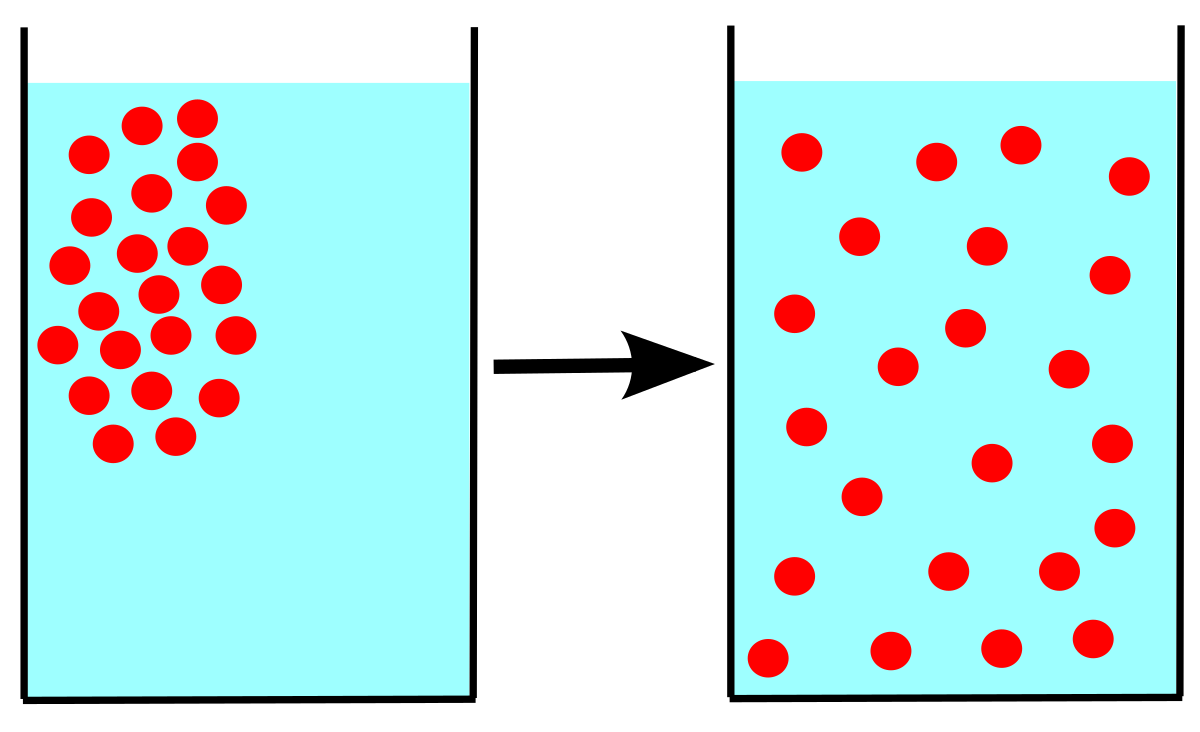
\includegraphics[scale=0.15]{./images/diffusion.png}
%		\caption{Disffusion.}
%		\label{fig:diffusion}
%	\end{figure}
% \vskip0pt plus 1filll
% \href{https://arxiv.org/abs/1503.03585}{\tiny \blue{ICML 2015 Deep Unsupervised Learning using Nonequilibrium Thermodynamics}}

	The overall idea is to construct a Markov chain of progressively less noisy samples. Each transition denoises a noisy sample. Diffusion models consist of two Markov chains:
	\begin{enumerate}
		\item Forward: A Markov chain of diffusion steps to \textbf{slowly add random noise} to data. 
			$$\rvx_0\to \rvx_1\cdots\to \rvx_T$$
		\item Backward (Reverse): Learn to \textbf{reverse the diffusion process} to construct desired data samples from the noise. 
			$$\rvx_T\to \rvx_{T-1}\cdots\to \rvx_0$$
	\end{enumerate}
	\begin{figure}[t]
		\centering
		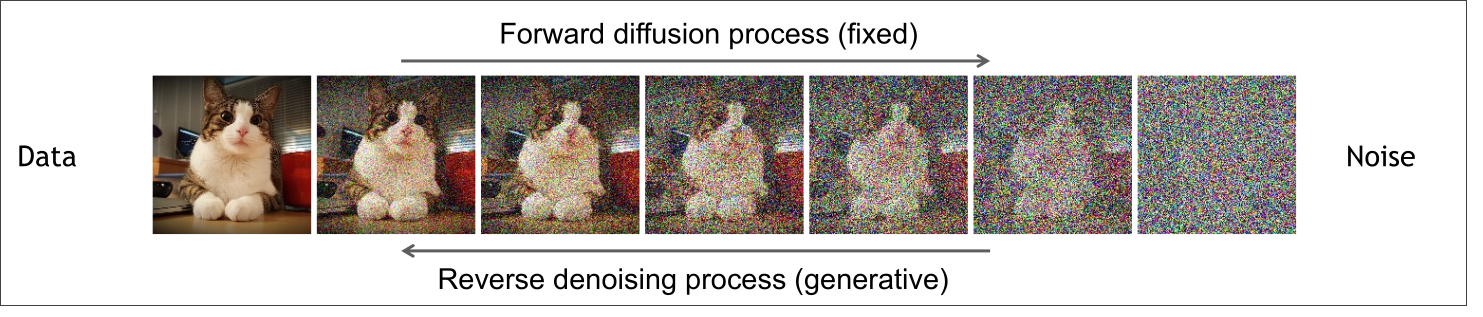
\includegraphics[scale=0.28]{./images/diffusion/diffusion_model.png}
	\end{figure}
	% \href{https://cvpr2022-tutorial-diffusion-models.github.io/}{\tiny \blue{CVRP 2022 Tutorial: Denoising Diffusion-based Generative Modeling: Foundations and Applications}}

\textbf{Some properties of diffusion models}:
	\begin{enumerate}
		%$$q(\rvx_t|\rvx_{t-1}) = \mathcal{T}(\rvx_t|\rvx_{t-1})$$
		\item Diffusion model has a pre-defined sampling equation.
			\begin{itemize}
				\item The equation relies on a random noise.
				\item Noise is all we need $\to$ Predict noise at a time step $t$.
			\end{itemize}
		\item Fit a model via forward and backward processes.
		\item \textbf{Iterative transform} of one distribution into another via \textbf{Makov Chain}.
			\begin{itemize}
				\item $\mathcal{D}_{data}\to \mathcal{N}$.
				\item $\mathcal{N}\to \mathcal{D}_{data}$.
				\item Diffusion model$\approx$Generative Markov Chain.
			\end{itemize}
		\item Learn a transition model:
			$$p_\theta(\mathbf{x}_{t-1}|x_t) = \mathcal{N}(\mathbf{x}_{t-1}|\boldsymbol{\mu}_{\theta}(\mathbf{x}_{t}, t), \boldsymbol{\Sigma}_\theta(\mathbf{x}_t,t)).$$
		\item Base case: $p(\mathbf{x}_T) = \mathcal{N}(0,I)$ 
		\item Marginal distribution over $\mathbf{x}_0$:
			$$p_\theta(\mathbf{x}_0) = \int p_\theta(\rvx_0,\dots,\mathbf{x}_T)d\rvx_1,\dots,\rvx_T$$
		\item We want to learn the parameters so that
			$$p(\rvx_0)\approx p_\theta(\rvx_0)$$

	\end{enumerate}

\section{Forward Diffusion}

	\begin{itemize}
		\item We want to model a forward trajectory (by the Markov property): 
			$$q(\mathbf{x}_{0:T}) = q(\rvx_0)\prod^T_{t=1} \underbrace{q(\mathbf{x}_t \vert \mathbf{x}_{t-1})}_{\text{Transition kernel}} $$
		\item Slow transform with a large $T$: $\rvx_0\to \rvx_1\cdots\to \rvx_T$
			\begin{itemize}
				\item Imagine someone said he is from Germany.
				\item We can't exactly track his journey without more information.
				\item We need to add more steps!
			\end{itemize}
		\item How to model $q(\mathbf{x}_t \vert \mathbf{x}_{t-1})$?
%		\item By the Markov property, $q$ is given by
%			$$q(\mathbf{x}_{1:T} \vert \mathbf{x}_0) &=  \prod^T_{t=1} q(\mathbf{x}_t \vert \mathbf{x}_{t-1})$$
		%\item $q(\mathbf{x}_t \vert \mathbf{x}_{t-1}) = $
	\end{itemize}

Forward Diffusion: $q(\rvx_t \vert \rvx_{t-1})$
	In a continuous case (\eg image), each transition can be parameterized as follows:
\begin{align}
	q(\rvx_t \vert \rvx_{t-1}) &= \mathcal{N}(\mathbf{x}_t; \sqrt{1 - \beta_t} \rvx_{t-1}, \beta_t\mathbf{I})
	\label{eq:forward_diffusion}
\end{align}
\begin{itemize}
		\item $\beta_t\in (0,1)$ is a variance at time $t$.
		\item $\sqrt{1 - \beta_t}$ downscales $\rvx_{t-1}$ to be 0, $\beta_1<\cdots<\beta_t$. Thus, $\rvx_t$ will become more noisier. $\rvx_t$ can be sampled as:
			$$\mathbf{x}_t= \sqrt{1 - \beta_t} \mathbf{x}_{t-1}+ \sqrt{\beta_t} \odot \epsilon$$
			\begin{enumerate}
				\item Sample $\rvx_{t}\sim q(\rvx_t)$ and scale it by $\sqrt{1 - \beta_t}$
				\item Adds noise $\epsilon\sim \mathcal{N}(0,I)$ with variance $\beta_t$.
			\end{enumerate}
		\item The above process is autoregressive (\ie ancestral sampling), but we can sample $\mathbf{x}_t$ directly from $q(\mathbf{x}_t|\rvx_0)$ in an analytic form:
\begin{align}
	\rvx_t &= \sqrt{1 - \beta_t} \mathbf{x}_{t-1}+ \sqrt{\beta_t} \odot \epsilon_{t-1}\\
						   &= \sqrt{\alpha_t} \mathbf{x}_{t-1}+ \sqrt{1-\alpha_t} \odot \epsilon_{t-1}\\
						   &= \sqrt{\alpha_t} \bigg(\sqrt{\alpha_{t-1}} \mathbf{x}_{t-2}+ \sqrt{1-\alpha_{t-1}} \odot \epsilon_{t-2}\bigg) + \sqrt{1-\alpha_t} \odot \epsilon_{t-1}\\
						   &= \sqrt{\alpha_t\alpha_{t-1}} \mathbf{x}_{t-2} + \sqrt{\alpha_t-\alpha_t\alpha_{t-1}} \odot \epsilon_{t-2} + \sqrt{1-\alpha_t} \odot \epsilon_{t-1}\\
						   &= \sqrt{\alpha_t\alpha_{t-1}} \mathbf{x}_{t-2} + \sqrt{\alpha_t-\alpha_t\alpha_{t-1}+1-\alpha_t} \odot \epsilon_{t-2} \\
						   &= \sqrt{\alpha_t\alpha_{t-1}} \mathbf{x}_{t-2} + \sqrt{1-\alpha_t\alpha_{t-1}} \odot \epsilon_{t-2} \\
						   &= \dots\\
						   &= \sqrt{\prod_{t}\alpha_t} \mathbf{x}_{0} + \sqrt{1-\prod_t \alpha_t} \odot \epsilon_{t_0} \\
						   &= \sqrt{\bar{\alpha}_t} \mathbf{x}_{0}+ \sqrt{1-\bar{\alpha}_t} \odot \epsilon\\
	&\sim \mathcal{N}(\mathbf{x}_t; \sqrt{\bar{\alpha}_t} \rvx_{0}, (1-\bar{\alpha}_t)\mathbf{I}),
	% &= q(\mathbf{x}_t|\rvx_{0}), 
	\label{eq:diffusion_forward_sampling}
\end{align}
			where $\alpha_t = 1-\beta_t$ and $\bar{\alpha}_t = \prod_{s=1}^t \alpha_s$. Thus, $\mathbf{x}_t= \sqrt{\bar{\alpha}_t} \mathbf{x}_{0}+ \sqrt{1-\bar{\alpha}_t} \odot \epsilon$. Note that the fifth step is done by using the property of sum of two Gaussian distributions (\eg $\mathcal{N}(0, \sigma_1^2I)+\mathcal{N}(0, \sigma_2^2I) = \mathcal{N}(0, (\sigma_1^2+\sigma_2^2)I)$ ). 
\end{itemize}

We can get some intuitions:
\begin{itemize}
	\item The original input $\rvx_0$ \textbf{gradually loses all info} during the forward diffusion process.
	\item This Markov chain has a \textbf{stationary distribution}: As $t\to \infty$, $q(\rvx_t) \approx \mathcal{N}(0,I)$.
		\begin{itemize}
			\item In practice, $T$ is a very high number \eg 1,000.
			\item Minimize info loss for each step.
			\item Allow a smooth training.
		\end{itemize}
\end{itemize}

%\begin{frame}{Forward Diffusion: $q(\rvx_t)$}
%	\begin{align*}
%		\underbrace{q(x_t)}_{\text{diffused data dist.}} = \int \underbrace{q(x_t,x_0)}_{\text{Joint dist.}} dx_0 = \int \underbrace{q(x_0)}_{\text{Input dist.}}\underbrace{q(x_t|x_0)}_{\text{Diffusion kernel}} dx_0 .
%	\end{align*}
%	\begin{itemize}
%		\item We can sample $\rvx_t\sim q(\rvx_t)$ by first sampling $\rvx_0\sim q(\rvx_0)$
%		\item Sample $\rvx_t$ at any arbitrary noise level without iterative computations.
%		\item $\rvx_t = \sqrt{\bar{\alpha}_t}\rvx_0+\sqrt{(1-\bar{\alpha}_t)}\epsilon$ : reparameterization
%		\item $\alpha_t:=1-\beta_t$
%		\item $\bar{\alpha}_t:=\prod_{i=1}^t\alpha_i$
%		\item \red{Why sampling $\rvx_t$?}
%	\end{itemize}
%\end{frame}

%\begin{frame}{Forward Diffusion}
%	\begin{itemize}
%		\item Diffusion kernel: 
%			$$q(x_t|x_0) = \mathcal{N}(\sqrt{\bar{\alpha}_t}x_0, (1-\bar{\alpha}_t)I )$$
%		\item[] $\approx$ Gaussian convolution.
%		\item We can sample $x_t$ by adding scaled noise to $x_0$.
%		\item $\beta_t$ value is scheduled to be $\bar{\alpha}_T\to 0$ and $q(x_t|x_0)\approx \mathcal{N}(x_T;0,I)$
%	\end{itemize}
%\end{frame}



\section{Backward Process}

Generative Learning by Denoising:
	\begin{itemize}
		\item Now we know how to model the forward process (diffusion process).
		\item However, a noisy image is not what we want.
		\item We want to generate a new image with high quality.
	\end{itemize}

	How to generate data? If we can reverse the forward process, then we can draw a true sample. We call it \textbf{Backward process}!
	\begin{itemize}
		\item Start from $q(\rvx_T)\approx \mathcal{N}(0,I)$.
		\item Sample $\rvx_T\sim \mathcal{N}(\rvx_T|0,I)$
			\begin{itemize}
				\item Sample a noise vector from a prior distribution.
			\end{itemize}
		\item Iteratively sample $\rvx_{t-1}\sim q(\rvx_{t-1}|\rvx_t).$ 
			\begin{itemize}
				\item $q(\rvx_{t-1}|\rvx_t)$: \textbf{true denoising distribution} (we don't know).
			\end{itemize}
		\item In general, $q(\rvx_{t-1}|\rvx_t)$ is intractable.
		%\item In general, $q(x_{t-1}|x_t)\propto q(x_{t-1})q(x_t|x_{t-1})$ is intractable.
		\item We can \textbf{approximate} $q(\rvx_{t-1}|\rvx_t)$ as \textbf{Normal distribution} if $\beta_t$ is small in each forward diffusion step.
			\begin{itemize}
				\item \eg $\rvx_3$ to $\rvx_2$
			\end{itemize}
	\end{itemize}
	\begin{figure}[h]
		\centering
		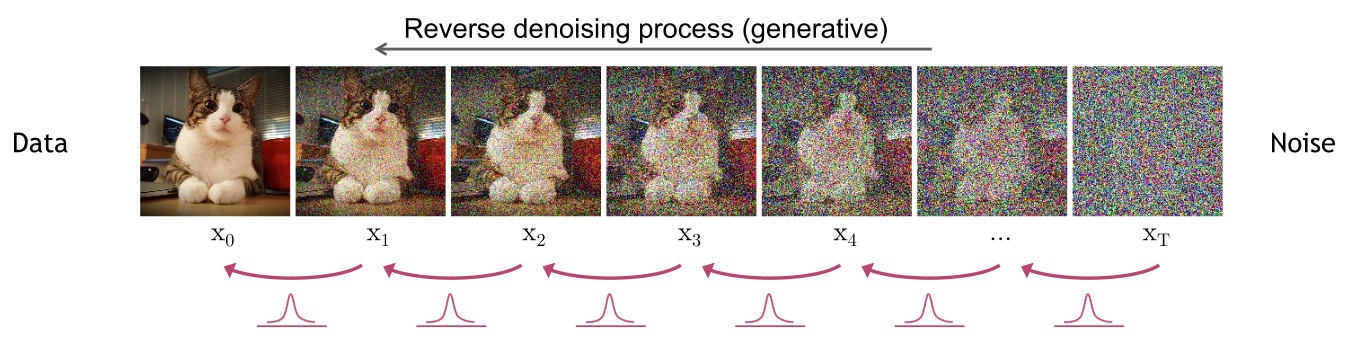
\includegraphics[scale=0.30]{./images/diffusion/reverse.png}
	\end{figure}
	\href{https://cvpr2022-tutorial-diffusion-models.github.io/}{\tiny \blue{CVPR 2022 Tutorial: Denoising Diffusion-based Generative Modeling: Foundations and Applications}}

Backward Process
	\begin{itemize}
%		\item Reverse the forward process
%			\begin{itemize}
%					\item Sample from the \textbf{exact reverse distribution} $q(\rvx_{t-1}|\rvx_t)$ (true denoising dist.), 
%					\item Recreate the true sample from a Gaussian noise input $\rvx_T\sim \mathcal{N}(0,I)$.
%				\end{itemize}
		%\item The reversal of the disffusion process has the identical form as the forward process.
		%\item The longer the trajectory the smaller the diffusion rate $\beta$ can be made.
		\item Approximate $q(\rvx_{t-1}|\rvx_t)$ using a neural network, $p_\theta(\mathbf{x}_{t-1} \vert \mathbf{x}_t)$.
		\item Backward process: $p_\theta(\mathbf{x}_{0:T}) = p(\mathbf{x}_T) \prod^T_{t=1} p_\theta(\mathbf{x}_{t-1} \vert \mathbf{x}_t)$.
			\begin{itemize}
				\item $p(\rvx_T) = \mathcal{N}(\rvx_T;0,I)$.
				\item $p_\theta(\mathbf{x}_{t-1} \vert \mathbf{x}_t) = \mathcal{N}(\mathbf{x}_{t-1}; \boldsymbol{\mu}_\theta(\mathbf{x}_t, t), \boldsymbol{\Sigma}_\theta(\mathbf{x}_t, t))$.  

				\item We can model the denoising distribution as Normal distribution like above (\cf \Cref{eq:diffusion_kl_true_denoising}).
				\item Note that the reverse conditional probability $q(\rvx_{t-1}|\rvx_t)$ is tractable when it is conditioned on $\rvx_0$ as shown in \Cref{eq:diffusion_kl_true_denoising}. This allows us to train a neural network to model this denoising distribution. 
			\end{itemize}
			% \begin{itemize}
			% 	\item Network outputs mean and variance ($\boldsymbol{\mu}_{\theta}$ and $\boldsymbol{\Sigma}_{\theta}$). 
			% 	\item We are not going to make a model to predict them directly.
			% 	\item \textbf{Train a noise prediction network.}
			% \end{itemize}
		\item Key to the success of this sampling process is training the reverse Markov chain to match the actual time reversal of the forward Markov chain. 
		\item After optimizing the backward process, the sampling procedure is that just sample Gaussian noise from $p(\rvx_T)$ and then iteratively running the denoising transitions (backward process) for T steps to generate a novel $\rvx_0$.
	\end{itemize}


\section{Distribution Modeling}
	What we want to learn (or model) is $p_\theta(\rvx_0)\approx p(\rvx_0)$ (approximate data distribution).
	\begin{itemize}
%		\item $p_\theta(\rvx_0)$: a distribution of output (denoised) image.
%			\begin{itemize}
%				\item This is our target.
%			\end{itemize}
		\item $p_\theta(\rvx_0) = \int p_\theta(\rvx_{0:T})d\rvx_{1:T}$
		\item It is intractable to compute all trajectories.
			$$\argmax_\theta\mathbb{E}_{\rvx_0\sim p}[\log p_\theta(\rvx_0)] = \mathbb{E}_{\rvx_0\sim p}\bigg[\log\int p_\theta(\rvx_{0:T})d\rvx_{1:T}\bigg].$$
		\item Thus, we will use variational lower bound with KL-Div:
	\end{itemize}
\begin{align}
\log p_\theta(\rvx_0) 
	&=  \log\int p(\rvx_{0:T})d\rvx_{1:T}\\
	&= \log\int p(\rvx_{0:T})\frac{q(\rvx_{1:T}|\rvx_0)}{q(\rvx_{1:T}|\rvx_0)}d\rvx_{1:T}\\
	&= \log\int q(\rvx_{1:T}|\rvx_0)\frac{p(\rvx_{0:T})}{q(\rvx_{1:T}|\rvx_0)}d\rvx_{1:T}\\
	&\geq \int q(\rvx_{1:T}|\rvx_0)\log\frac{p(\rvx_{0:T})}{q(\rvx_{1:T}|\rvx_0)}d\rvx_{1:T}\\
	&= \mathbb{E}_{q(\rvx_{1:T}|\rvx_0)}\bigg[\log\frac{p(\rvx_{0:T})}{q(\rvx_{1:T}|\rvx_0)}\bigg] \quad \to \textrm{ELBO}\\
	&= \mathbb{E}_{q(\rvx_{1:T}|\rvx_0)}\bigg[\log p(\rvx_T)\prod_{t=1}^T\frac{p(\rvx_{t-1}|\rvx_t)}{q(\rvx_{t}|\rvx_{t-1})}\bigg]\\
	&= \mathbb{E}_{q(\rvx_{1:T}|\rvx_0)}\bigg[\log \frac{p(\rvx_T)p(\rvx_0|\rvx_{1})\prod_{t=1}^{T-1} p(\rvx_{t}|\rvx_{t+1})}{q(\rvx_T|\rvx_{T-1})\prod_{t=1}^{T-1}  q(\rvx_{t}|\rvx_{t-1})}\bigg]\\
	&= \mathbb{E}_{q(\rvx_{1:T}|\rvx_0)}\bigg[\log \frac{p(\rvx_T)p(\rvx_0|\rvx_{1})}{q(\rvx_T|\rvx_{T-1})}\bigg] + \mathbb{E}_{q(\rvx_{1:T}|\rvx_0)}\bigg[\log \prod_{t=1}^{T-1}\frac{ p(\rvx_{t}|\rvx_{t+1})}{q(\rvx_{t}|\rvx_{t-1})}\bigg]\\
	&= \mathbb{E}_{q(\rvx_{1:T}|\rvx_0)}[\log p(\rvx_0|\rvx_{1})]+\mathbb{E}_{q(\rvx_{1:T}|\rvx_0)}\bigg[\log \frac{p(\rvx_T)}{q(\rvx_T|\rvx_{T-1})}\bigg]\\ 
	&\quad + \mathbb{E}_{q(\rvx_{1:T}|\rvx_0)}\bigg[\sum_{t=1}^{T-1}\log \frac{ p(\rvx_{t}|\rvx_{t+1})}{q(\rvx_{t}|\rvx_{t-1})}\bigg]\\
	&= \dots + \blue{\mathbb{E}_{q(\rvx_{1:T}|\rvx_0)}\bigg[\log \frac{p(\rvx_T)}{q(\rvx_T|\rvx_{T-1})}\bigg]} + \sum_{t=1}^{T-1}\mathbb{E}_{q(\rvx_{1:T}|\rvx_0)}\bigg[\log \frac{ p(\rvx_{t}|\rvx_{t+1})}{q(\rvx_{t}|\rvx_{t-1})}\bigg]\\
	% % &= \log\int q(\rvx_{1:T}|\rvx_0)p(\rvx_T)\prod_{t=1}^T\frac{p(\rvx_{t-1}|\rvx_t)}{q(\rvx_{t}|\rvx_{t-1})}d\rvx_{1:T}
		&= \dots + \int_{x_1}\dots\int_{x_T}q(\rvx_{1},\dots,\rvx_{T})\bigg[\log \frac{p(\rvx_T)}{q(\rvx_T|\rvx_{T-1})}\bigg]dx_1\dots dx_T + \dots\\
		&= \dots + \int_{x_T}\int_{x_{T-1}}\bigg[\log \frac{p(\rvx_T)}{q(\rvx_T|\rvx_{T-1})}\bigg]\dots\int_{x_1} q(\rvx_{1},\dots,\rvx_{T})dx_1\dots dx_T + \dots\\
		&= \dots + \int_{x_T}\int_{x_{T-1}}\bigg[\log \frac{p(\rvx_T)}{q(\rvx_T|\rvx_{T-1})}\bigg] q(\rvx_{t},\rvx_{t-1})dx_{T-1} dx_T + \dots\\
		&= \dots + \mathbb{E}_{q(\rvx_{t}, \rvx_{t-1}|\rvx_0)}\bigg[\log \frac{p(\rvx_T)}{q(\rvx_T|\rvx_{T-1})}\bigg] + \sum_{t=1}^{T-1}\mathbb{E}_{q(\rvx_{t-1},\rvx_t,\rvx_{t+1}|\rvx_0)}\bigg[\log \frac{ p(\rvx_{t}|\rvx_{t+1})}{q(\rvx_{t}|\rvx_{t-1})}\bigg]\\
		&= \mathbb{E}_{q(\rvx_{1}|\rvx_0)}[\log p(\rvx_0|\rvx_{1})] + \mathbb{E}_{q(\rvx_{t}, \rvx_{t-1}|\rvx_0)}\bigg[\log \frac{p(\rvx_T)}{q(\rvx_T|\rvx_{T-1})}\bigg]\\ 
		&\quad+ \sum_{t=1}^{T-1}\mathbb{E}_{q(\rvx_{t-1},\rvx_t,\rvx_{t+1}|\rvx_0)}\bigg[\log \frac{ p(\rvx_{t}|\rvx_{t+1})}{q(\rvx_{t}|\rvx_{t-1})}\bigg]\\
		&= \mathbb{E}_{q(\rvx_{1}|\rvx_0)}[\log p(\rvx_0|\rvx_{1})] - \mathbb{E}_{q(\rvx_{t-1}|\rvx_0)}[D_{KL}(q(\rvx_T|\rvx_{T-1})\| p(\rvx_T))]\\
		&\,- \sum_{t=1}^{T-1}\mathbb{E}_{q(\rvx_{t-1},\rvx_{t+1}|\rvx_0)}D_{KL}[q(\rvx_{t}|\rvx_{t-1})\|p(\rvx_{t}|\rvx_{t+1})]\\
		& \because q(\rvx_{t}, \rvx_{t-1}|\rvx_0) = \frac{q(\rvx_{t}, \rvx_{t-1},\rvx_0)}{q(\rvx_0)} = \frac{q(\rvx_{t}|\rvx_{t-1}, \rvx_0)q(\rvx_{t-1}, \rvx_0)}{q(\rvx_0)} = q(\rvx_{t}|\rvx_{t-1})q(\rvx_{t-1}|\rvx_0)
	% % &= \log\int q(\rvx_{1:T}|\rvx_0)p(\rvx_T)\prod_{t=1}^T\frac{p(\rvx_{t-1}|\rvx_t)}{q(\rvx_{t}|\rvx_{t-1})}d\rvx_{1:T}
	\label{eq:diffusion_mle}
\end{align}
\begin{itemize}
	\item The sixth step is done by Markov property.
	\item The first term is a \textit{reconstruction term}. 
	\item The second term is a \textit{prior matching term}. This term requires no optimization, as it has no trainable parameters; furthermore, as we have assumed a large enough $T$ such that the final distribution is Gaussian, this term effectively becomes zero.
	\item The last term is a \textit{consistency term}. It endeavors to make the distribution at xt consistent, from both forward and backward processes. That is, a denoising step from a noisier image should match the corresponding noising step from a cleaner image, for every intermediate timestep.  This term is minimized when we train $p_\theta(\rvx_t|\rvx_{t+1})$ to match the Gaussian distribution $q(\rvx_t|\rvx_{t-1})$, which is defined in \Cref{eq:forward_diffusion}. % \item For a small $\beta$, the forward and the backward processes can be identical.
	\item Under this derivation, all terms of the ELBO are computed as expectations, and can therefore be approximated using Monte Carlo estimates. 
	\item However, actually optimizing the ELBO using the terms we just derived might be suboptimal, because the consistency term is computed as an expectation over two random variables $\{x_{t-1}, x_{t+1}\}$ for every time step, the variance of its Monte Carlo estimate could potentially be higher than a term that is estimated using only one random variable per time step. As it is computed by summing up $T-1$ consistency terms, the final estimated value of the ELBO may have high variance for large $T$ values.
\end{itemize}

Let us instead try to derive a form for our ELBO where each term is computed as an expectation over \textbf{only one random variable at a time}. The key insight is that we can rewrite encoder transitions as $q(x_t|x_{t-1}) = q(x_t|x_{t-1}, x_0)$, where the extra conditioning term is superfluous due to the Markov property. Then, according to Bayes rule, we can rewrite each transition as:
\begin{align*}
	q(\rvx_t|\rvx_{t-1}, \rvx_0)= \frac{q(\rvx_{t-1}|\rvx_t, \rvx_0)q(\rvx_t| \rvx_0)}{q(\rvx_{t-1}| \rvx_0)} 
\end{align*}
Armed with this equation, we can factorize the ELBO again as follows:
\begin{align}
		L &= \mathbb{E}_{q(\rvx_{1:T}|\rvx_0)}\bigg[\log\frac{p(\rvx_{0:T})}{q(\rvx_{1:T}|\rvx_0)}\bigg] \quad \to \textrm{ELBO}\\		
		&= \mathbb{E}_{q(\rvx_{1:T}|\rvx_0)}\bigg[\log p(\rvx_T)\prod_{t=1}^T\frac{p(\rvx_{t-1}|\rvx_t)}{q(\rvx_{t}|\rvx_{t-1})}\bigg]\\
		&= \mathbb{E}_{q(\rvx_{1:T}|\rvx_0)}\bigg[\log \frac{p(\rvx_T)p(\rvx_0|\rvx_{1})\prod_{t=2}^{T} p(\rvx_{t-1}|\rvx_{t})}{q(\rvx_1|\rvx_{0})\prod_{t=2}^{T}  q(\rvx_{t}|\rvx_{t-1})}\bigg]\\
		&= \mathbb{E}_{q(\rvx_{1:T}|\rvx_0)}\bigg[\log \frac{p(\rvx_T)p(\rvx_0|\rvx_{1})\prod_{t=2}^{T} p(\rvx_{t-1}|\rvx_{t})}{q(\rvx_1|\rvx_{0})\prod_{t=2}^{T}  q(\rvx_{t}|\rvx_{t-1}, \blue{\rvx_0})}\bigg] \quad \textrm{ by Markov Property}\\
		&= \mathbb{E}_{q(\rvx_{1:T}|\rvx_0)}\bigg[\log \frac{p(\rvx_T)p(\rvx_0|\rvx_{1})}{q(\rvx_1|\rvx_{0})}+\log \prod_{t=2}^{T}\frac{ p(\rvx_{t-1}|\rvx_{t})}{q(\rvx_{t}|\rvx_{t-1}, \rvx_0)}\bigg]\\
		&= \mathbb{E}_{q(\rvx_{1:T}|\rvx_0)}\bigg[\log \frac{p(\rvx_T)p(\rvx_0|\rvx_{1})}{q(\rvx_1|\rvx_{0})}+\log \prod_{t=2}^{T}\frac{ p(\rvx_{t-1}|\rvx_{t})}{\frac{q(\rvx_{t-1}|\rvx_t, \rvx_0)q(\rvx_t| \rvx_0)}{q(\rvx_{t-1}| \rvx_0)}}\bigg]\\
		&= \mathbb{E}_{q(\rvx_{1:T}|\rvx_0)}\bigg[\log \frac{p(\rvx_T)p(\rvx_0|\rvx_{1})}{q(\rvx_1|\rvx_{0})}+\log \frac{q(\rvx_1|\rvx_0)}{q(\rvx_T|\rvx_0)}+\log \prod_{t=2}^{T}\frac{ p(\rvx_{t-1}|\rvx_{t})}{q(\rvx_{t-1}|\rvx_t, \rvx_0)}\bigg]\\
		&= \mathbb{E}_{q(\rvx_{1:T}|\rvx_0)}\bigg[\log \frac{p(\rvx_T)p(\rvx_0|\rvx_{1})}{q(\rvx_T|\rvx_{0})}+\log \prod_{t=2}^{T}\frac{ p(\rvx_{t-1}|\rvx_{t})}{q(\rvx_{t-1}|\rvx_t, \rvx_0)}\bigg]\\
		&= \mathbb{E}_{q(\rvx_{1}|\rvx_0)}[\log p(\rvx_0|\rvx_{1})]+\mathbb{E}_{q(\rvx_{T}|\rvx_0)}\bigg[\log \frac{p(\rvx_T)}{q(\rvx_T|\rvx_{0})}\bigg]+\ \sum_{t=2}^{T}\mathbb{E}_{q(\rvx_{t},\rvx_{t-1}|\rvx_0)}\bigg[\log\frac{ p(\rvx_{t-1}|\rvx_{t})}{q(\rvx_{t-1}|\rvx_t, \rvx_0)}\bigg]\\
		&= \mathbb{E}_{q(\rvx_{1}|\rvx_0)}[\log p(\rvx_0|\rvx_{1})]-D_{KL}_(q(\rvx_{T}|\rvx_0)||p(\rvx_T))-\sum_{t=2}^{T}\mathbb{E}_{q(\rvx_{t}|\rvx_0)}[D_{KL}(q(\rvx_{t-1}|\rvx_t, \rvx_0)\|p(\rvx_{t-1}|\rvx_{t}))]
		% &= \mathbb{E}_{q(\rvx_{1:T}|\rvx_0)}\bigg[\log \frac{p(\rvx_T)p(\rvx_0|\rvx_{1})}{q(\rvx_T|\rvx_{T-1})}\bigg] + \mathbb{E}_{q(\rvx_{1:T}|\rvx_0)}\bigg[\log \prod_{t=1}^{T-1}\frac{ p(\rvx_{t}|\rvx_{t+1})}{q(\rvx_{t}|\rvx_{t-1})}\bigg]\\
% 		&= \mathbb{E}_{q}\Bigg[-\log p_\theta(x_T)-\log\frac{\prod_{t=1}^Tp_\theta(x_{t-1}|x_t)}{\prod_{t=1}^Tq(x_{t}|x_{t-1})}\Bigg]\\
% 		&= \mathbb{E}_{q}\Bigg[-\log p_\theta(x_T)-\sum_{t\geq 1}\log\frac{p_\theta(x_{t-1}|x_t)}{q(x_{t}|x_{t-1})}\Bigg]\\
% 		&= \mathbb{E}_{q}\Bigg[-\log p_\theta(x_T)-\sum_{t=2}^T\log\frac{p_\theta(x_{t-1}|x_t)}{q(x_{t}|x_{t-1})}-\log \frac{p_\theta(x_{0}|x_1)}{q(x_{1}|x_{0})}\Bigg]\\
% 		&= \mathbb{E}_{q}\Bigg[-\log p_\theta(x_T)-\sum_{t=2}^T\log\frac{p_\theta(x_{t-1}|x_t)}{q(x_{t-1}|x_{t},x_0)}\cdot \red{ \frac{q(x_{t-1}|x_0)}{q(x_{t}|x_0)}}\\
% 		&\quad -\log \frac{p_\theta(x_{0}|x_1)}{q(x_{1}|x_{0})}\Bigg]\\
	\label{eq:diffusion_objective}
\end{align}
Let's closely look at the last three terms:
\begin{itemize}
	\item $\mathbb{E}_{q(\rvx_{1}|\rvx_0)}[\log p(\rvx_0|\rvx_{1})]$: reconstruction term. 
	\item $D_{KL} (q(\rvx_{T}|\rvx_0)||p(\rvx_T))$: Prior matching term.
		\begin{itemize}
			\item No trainable parameters 
		\end{itemize}
	\item $\sum_{t=2}^{T}\mathbb{E}_{q(\rvx_{t}|\rvx_0)}[D_{KL}(q(\rvx_{t-1}|\rvx_t, \rvx_0)\|p(\rvx_{t-1}|\rvx_{t}))]$: Denoising matching term.
		\begin{itemize}
			\item $p_\theta(\rvx_{t−1}|\rvx_t)$ as an approximation to tractable, ground-truth denoising transition step $q(\rvx_{t−1}|\rvx_t, \rvx_0)$. The $q(\rvx_{t−1}|\rvx_t, \rvx_0)$ transition step can act as a ground-truth signal, since it defines how to denoise a noisy image with access to what the final, completely denoised image $\rvx_0$ should be. This term is therefore minimized when the two denoising steps match as closely as possible, as measured by their KL Divergence.
		\end{itemize}
\end{itemize}
In the last term, $q(\rvx_{t-1}|\rvx_t, \rvx_0)$ can be further factorized as follows:
\begin{align*}
	q(\rvx_{t-1}|\rvx_t, \rvx_0) = \frac{q(\rvx_{t}|\rvx_{t-1}, \rvx_0)q(\rvx_{t-1}|\rvx_0)}{q(\rvx_{t}|\rvx_0)}=\frac{q(\rvx_{t}|\rvx_{t-1})q(\rvx_{t-1}|\rvx_0)}{q(\rvx_{t}|\rvx_0)}.
\end{align*}
Then, $q(\rvx_{t}|\rvx_{t-1}, \rvx_0) = q(\rvx_{t}|\rvx_{t-1})$ by Markov property. Now, let's compute the KL-divergence in the denoising matching term. 

\begin{align}
	q(\rvx_{t-1}|\rvx_t, \rvx_0) &=\frac{q(\rvx_{t}|\rvx_{t-1})q(\rvx_{t-1}|\rvx_0)}{q(\rvx_{t}|\rvx_0)}\\
								 &= \frac{\mathcal{N}(\mathbf{x}_t; \sqrt{\bar{\alpha}_t} \rvx_{t-1}, (1-\bar{\alpha}_t)\mathbf{I})\mathcal{N}(\mathbf{x}_{t-1}; \sqrt{\bar{\alpha}_{t-1}} \rvx_{0}, (1-\bar{\alpha}_{t-1})\mathbf{I})}{\mathcal{N}(\mathbf{x}_t; \sqrt{\bar{\alpha}_t} \rvx_{0}, (1-\bar{\alpha}_t)\mathbf{I})}\\
								 & \vdots\\
								 &\propto \mathcal{N}\bigg(\rvx_{t-1};\underbrace{\frac{\sqrt{{\alpha}_{t}}(1-\bar{\alpha}_{t-1})\rvx_t+\sqrt{\bar{\alpha}_{t-1}}(1-{\alpha}_{t})\rvx_0}{1-\bar{\alpha}_{t}}}_{\mu_q(\rvx_t,\rvx_0)}, \underbrace{\frac{(1-{\alpha}_{t})(1-\bar{\alpha}_{t-1})}{1-\bar{\alpha}_{t}}\mathbf{I}}_{\Sigma_{q}(t)}\bigg)
	\label{eq:diffusion_kl_true_denoising}
\end{align}

We have therefore shown that at each step, $\rvx_{t-1} \sim q(\rvx_{t-1}|\rvx_t, \rvx_0)$ is normally distributed, with mean $\mu_q(\rvx_t,\rvx_0)$ that is a function of $\rvx_t$ and $\rvx_0$, and variance $\Sigma_q(t)$ as a function of $\alpha$ coefficients. 

% These $\alpha$ coefficients are known and fixed at each time step; they are either set permanently when modeled as hyperparameters, or treated as the current inference output of a network that seeks to model them. We can rewrite the variance equation as $\Sigma_q(t) = \sigma^2_q(t)I$, where:
% $$\sigma^2_q(t) = \frac{(1-{\alpha}_{t})(1-\bar{\alpha}_{t-1})}{1-\bar{\alpha}_{t}}.$$
% In order to match approximate denoising transition step $p_\theta(\rvx_{t-1}|\rvx_{t})$ to ground-truth denoising transition step $q(\rvx_{t-1}|\rvx_t, \rvx_0)$ as closely as possible, we can also model it as a Gaussian. Furthermore, as all $\alpha$ terms are known to be frozen at each timestep, we can immediately construct the variance of the approximate denoising transition step to also be $\Sigma_q(t) = \sigma^2_q(t)I$.

% The following equation is the KL divergence between two normal distributions $P$ and $Q$:
% $$D_{KL}(P\|Q) = \frac{1}{2}\left[\log\frac{|\Sigma_2|}{|\Sigma_1|} - n + \text{tr} \{ \Sigma_2^{-1}\Sigma_1 \} + (\mu_2 - \mu_1)^T \Sigma_2^{-1}(\mu_2 - \mu_1)\right]$$
% We can optimize the KL divergence between two normal distributions to minimize the difference between the two means: 
% \begin{align}
% 	\mathcal{L} &= \min_\theta D_{KL}(q(\rvx_{t-1}|\rvx_t, \rvx_0)\|p_\theta(\rvx_{t-1}|\rvx_{t}))\\
% 				& \vdots\\
% 				&= \min_\theta \frac{1}{2\sigma^2_q(t)}\big[\|\boldsymbol{\mu}_\theta- \boldsymbol{\mu}_q\|^2_2\big],
% 	\label{eq:diffusion_kl_mean}
% \end{align}
% where $\boldsymbol{\mu}_q$ is a shorthand for $\boldsymbol{\mu}_q(\rvx_t,\rvx_0)$.

We can use the \Cref{eq:diffusion_kl_true_denoising} to compute the optimal $\theta$ by solving $\min_\theta D_{KL}(q(\rvx_{t-1}|\rvx_t, \rvx_0)\|p_\theta(\rvx_{t-1}|\rvx_{t}))$, but we can simplify the optimization problem by using \Cref{eq:diffusion_forward_sampling}:
\begin{align*}
	\rvx_t &= \sqrt{\bar{\alpha}_t} \mathbf{x}_{0}+ \sqrt{1-\bar{\alpha}_t} \odot \epsilon\\
	\mathbf{x}_{0} &= \frac{\rvx_t - \sqrt{1-\bar{\alpha}_t}\odot \epsilon}{\sqrt{\bar{\alpha}_t} } 
\end{align*}
By plugging the above equation into $\boldsymbol{\mu}_q(\rvx_t,\rvx_0)$, we can exclude $\rvx_0$ term as follows:
\begin{align}
	\boldsymbol{\mu}_q(\rvx_t,\rvx_0) &= \frac{\sqrt{{\alpha}_{t}}(1-\bar{\alpha}_{t-1})\rvx_t+\sqrt{\bar{\alpha}_{t-1}}(1-{\alpha}_{t})\rvx_0}{1-\bar{\alpha}_{t}}\\
									  &= \frac{\sqrt{{\alpha}_{t}}(1-\bar{\alpha}_{t-1})\rvx_t+\sqrt{\bar{\alpha}_{t-1}}(1-{\alpha}_{t})\frac{\rvx_t - \sqrt{1-\bar{\alpha}_t}\odot \epsilon}{\sqrt{\bar{\alpha}_t} }}{1-\bar{\alpha}_{t}}\\
									  &\vdots\\
									  &= \frac{1}{\sqrt{\alpha_t}}\rvx_t - \frac{1-\alpha_t}{\sqrt{1-\bar{\alpha_t}}\sqrt{\alpha_t}}\boldsymbol{\epsilon}_0
	\label{eq:diffusion_mean_simple}
\end{align}
Thus, we can force $\boldsymbol{\mu}_\theta(\mathbf{x}_t, t)$, which has no dependency on $\rvx_0$ term, to match the $\boldsymbol{\mu}_q$. Since the $\rvx_t$ is given at training time, we just need to predict the $\boldsymbol{\epsilon}_t$. Then, we can express $\boldsymbol{\mu}_\theta(\mathbf{x}_t, t)$ as follows:
\begin{align*}
\boldsymbol{\mu}_\theta(\mathbf{x}_t, t) &= \frac{1}{\sqrt{\alpha_t}} \bigg( \mathbf{x}_t - \frac{1 - \alpha_t}{\sqrt{1 - \bar{\alpha}_t}} \boldsymbol{\epsilon}_\theta(\mathbf{x}_t, t) \bigg) \\
\end{align*}
Thus, $\rvx_{t-1}\sim p_\theta(\mathbf{x}_{t-1} \vert \mathbf{x}_t)$ can be expressed as follows:
\begin{align*}
	\mathcal{N}\Bigg(\mathbf{x}_{t-1}; \frac{1}{\sqrt{\alpha_t}} \bigg( \mathbf{x}_t - \frac{1 - \alpha_t}{\sqrt{1 - \bar{\alpha}_t}} \boldsymbol{\epsilon}_\theta(\mathbf{x}_t, t) \bigg), \boldsymbol{\Sigma}_\theta(\mathbf{x}_t, t)\Bigg)
\end{align*}
Note that we can use the variance derived in \Cref{eq:diffusion_kl_true_denoising} instead of estimating it from a network for simplicity. Finally, we can solve the KL-divergence term:

\begin{align}
	\mathcal{L} &= \min_\theta D_{KL}(q(\rvx_{t-1}|\rvx_t, \rvx_0)\|p_\theta(\rvx_{t-1}|\rvx_{t}))\\
				& \vdots\\
				&= \min_\theta \frac{1}{2\sigma^2_q(t)}\frac{(1-\alpha_t)^2}{(1-\bar{\alpha}_t)\alpha_t}\big[\|\boldsymbol{\epsilon}_0- \hat{\boldsymbol{\epsilon}}_\theta(\rvx_t,t)\|^2_2\big].
	\label{eq:diffusion_kl_mean_simple}
\end{align}
Here $\hat{\boldsymbol{\epsilon}}_\theta(\rvx_t,t)$ is a is a neural network that learns to predict the source noise $\boldsymbol{\epsilon}_0 \sim \mathcal{N}(\boldsymbol{\epsilon}}; \mathbf{0}, \mathbf{I})$ that determines $\rvx_t$ from $\rvx_0$. We have therefore shown that the overall learning objective is equivalent to learning to predict the noise.



\section{Summary}
\begin{itemize}
	\item The loss function can be decomposed.
		$$L_\text{VLB} = L_T + L_{T-1} + \dots + L_0 .$$
	\item $L_T = D_\text{KL}(q(\mathbf{x}_T \vert \mathbf{x}_0) \parallel p_\theta(\mathbf{x}_T))$
		\begin{itemize}
			\item Constant $\approx 0$ since $x_T$ is a Gaussian noise.
		\end{itemize}
	\item $L_t = D_\text{KL}(q(\mathbf{x}_{t-1} \vert \mathbf{x}_{t}, \mathbf{x}_0) \parallel p_\theta(\mathbf{x}_{t-1} \vert\mathbf{x}_{t})) \text{ for } t>1 $
	%\item $L_t = D_\text{KL}(q(\mathbf{x}_t \vert \mathbf{x}_{t+1}, \mathbf{x}_0) \parallel p_\theta(\mathbf{x}_t \vert\mathbf{x}_{t+1})) \text{ for }1 \leq t \leq T-1 $
		\begin{itemize}
			\item This is the main part.
		\end{itemize}
	\item $L_0 = - \log p_\theta(\mathbf{x}_0 \vert \mathbf{x}_1)$
		\begin{itemize}
			\item Can be modeled by a separate decoder.
		\end{itemize}
	\item $q(\rvx_t|\rvx_0) = \mathcal{N}(\sqrt{\bar{\alpha}_t}\rvx_0, (1-\bar{\alpha}_t)I )$
	\item $q(\rvx_t \vert \rvx_{t-1}) &= \mathcal{N}(\mathbf{x}_t; \sqrt{1 - \beta_t}\rvx_{t-1}, \beta_t\mathbf{I}),$
		\begin{itemize}
			\item[] We can sample by $\rvx_t=\sqrt{1 - \beta_t}\rvx_{t-1}+ \sqrt{\beta_t}\epsilon$
		\end{itemize}
	\item $p_\theta(\mathbf{x}_{t-1} \vert \mathbf{x}_t) = \mathcal{N}(\mathbf{x}_{t-1}; \boldsymbol{\mu}_\theta(\mathbf{x}_t, t), \boldsymbol{\Sigma}_\theta(\mathbf{x}_t, t))$.
		\begin{itemize}
			\item We need to learn mean and variance.
			\item DDPM kept the variance fixed and let the neural network only learn the mean $\mu_\theta$.
			\item $\boldsymbol{\Sigma}_\theta(\mathbf{x}_t, t)) = \sigma_t^2\mathbf{I}$ and set $\sigma_t^2 = \beta_t$.
		\item Improved DDPM model trains $\sigma$ also.
		\end{itemize}
	\item One can reparameterize the mean to make the nerual network learn the added noise via a network $\epsilon_\theta$.
		$$\mu_\theta(\rvx_t, t) = \frac{1}{\sqrt{\alpha_t}}\bigg(\rvx_t - \frac{\beta_t}{\sqrt{1-\bar{\alpha}_t}}\underbrace{\epsilon_\theta(\rvx_t,t)}_{\text{Network}}\bigg)$$
	\item Final objective function $L_t$ is
		$$||\epsilon -\epsilon_\theta(\rvx_t,t)||^2 = ||\epsilon -\epsilon_\theta(\sqrt{\bar{\alpha}_t}\rvx_0+\sqrt{(1-\bar{\alpha}_t)}\epsilon,t)||^2 $$
		\begin{itemize}
			\item $t\sim\text{Unif}[\{1,..,T\}]$ 
			\item $\rvx_t=\sqrt{\bar{\alpha}_t}\rvx_0+\sqrt{(1-\bar{\alpha}_t)}\epsilon \sim q(\rvx_t|\rvx_0)$
			\item $\epsilon\sim \mathcal{N}(0,I)$
		\end{itemize}
	\item $\rvx_t$ is perturbed by $\epsilon$ and the noise prediction network $\epsilon_\theta$ predicts $\epsilon$.
\end{itemize}

\newpage
\begin{algorithm}[t]
	\begin{algorithmic}[1]
		\Repeat
			\State $\rvx_0\sim q(\rvx_0)$
			\State $t\sim \text{Unif}[\{1,\cdots,T\}]$
			\State $\epsilon\sim \mathcal{N}(0,I)$
			\State Take gradient descent step on
			$\nabla_\theta||\epsilon -\epsilon_\theta(\sqrt{\bar{\alpha}_t}\rvx_0+\sqrt{(1-\bar{\alpha}_t)}\epsilon,t)||^2 $
		\Until converged
	\end{algorithmic}
	\caption{Training}
	\label{alg:diffusion_training}
\end{algorithm}

The training process is given by
\begin{enumerate}
	\item $\rvx_0\sim q(\rvx_0)$ 
	\item Sample a noise level $t$ between $1$ and $T$ (\ie random time step).
	\item Sample a noise from a Gaussian distribution and perturb the input by the sampling equation.
	\item NN is trained to predict this noise $\epsilon$ used for generating $\rvx_t$.
	\item $\beta$ is often scheduled linearly.
	\item $\Sigma$ is set equal to $\beta$.
\end{enumerate}

The sampling process is given by
\begin{algorithm}[h]
	\begin{algorithmic}[1]
		\State $\rvx_T\sim \mathcal{N}(0,I)$
		\For{$t=T,\cdots,1$}
			\State $\rvz\sim \mathcal{N}(0,I)$
			\State $\rvx_{t-1}= \frac{1}{\sqrt{\alpha_t}}\bigg(\rvx_t-\frac{1-\alpha_t}{\sqrt{1-\bar{\alpha}_t}}\boldsymbol{\epsilon}_\theta(\rvx_t,t)\bigg)+\Sigma_t\rvz$
		\EndFor
		\State \textbf{return} $\rvx_0$
	\end{algorithmic}
	\caption{Sampling}
	\label{alg:diffusion_sampling}
\end{algorithm*}
\begin{itemize}
	\item Ancestral sampling.
	\item $T$ is typically around 1,000
\end{itemize}
	

\section{Score Matching}
\begin{itemize}
	\item Suppose $\{\rvx_0,\cdots,\rvx_N\}$, where each data point (\eg image, video, or text)) is sampled independently from a data distribution $p(\rvx)$. 
	\item Given the dataset, the goal of generative modeling is to fit a model to the data distribution such that we can synthesize new data points at will by sampling from the model. 
	\item One way is to directly model the distribution function as in likelihood-based models. Let $f_\theta(\rvx)\in \mathbb{R}^d$, then we can define a density function:
	$$p_\theta(\rvx) = \frac{\exp^{-f_{\theta}(\rvx)}}{Z_\theta}$$.
	\item $f_\theta(\rvx)\in \mathbb{R}^d$ is often called unnormalized probabilistic model or energy-based model.
	\item Energy-based model originates from the Gibbs distribution in statistical physics.
	\item $p_\theta(\rvx)$ can be trained by maximizing the log-likelihood of the data.
		\begin{align*}
			\max_\theta \sum_i^N \log p_\theta(\rvx_i).
		\end{align*}
	\item The gradient of the loglikelihood is given by
		\begin{align*}
			\nabla_\theta \log p_\theta(\rvx) &= \nabla_\theta f_\theta(\rvx)- \nabla_\theta Z_\theta\\
			\nabla_\theta Z_\theta	&= \frac{\nabla_\theta Z_\theta}{ Z_\theta}\\
									&= \frac{1}{ Z_\theta}\nabla_\theta \int\exp(f_\theta(\rvx))d\rvx \\
									&= \frac{1}{ Z_\theta} \int\exp(f_\theta(\rvx))\nabla_\theta f_\theta(\rvx)d\rvx \\
									&=  \int \frac{1}{ Z_\theta}\exp(f_\theta(\rvx))\nabla_\theta f_\theta(\rvx)d\rvx \\
									&=  \int p_\theta(\rvx)\nabla_\theta f_\theta(\rvx)d\rvx \\
									&=  \mathbb{E}_{p_\theta(\rvx)}[\nabla_\theta f_\theta(\rvx)] \\
			\nabla_\theta \log p_\theta(\rvx) &= \nabla_\theta f_\theta(\rvx) - \mathbb{E}_{p_\theta(\rvx)}[\nabla_\theta f_\theta(\rvx)]
		\end{align*}
	\item However, it is undesirable, since $Z_\theta$ is intractable.
		\begin{itemize}
			\item For instance, a gray scale image of $100\times 100$ has $256^{10,000}$ space. 
		\end{itemize}
	\item Thus, we have to sidestep the issue by using some solutions, for instance:
		\begin{itemize}
			% \item Architecture: NMF
			\item Approximate by using VAE or MCMC
		\end{itemize}
\end{itemize}

Instead, we can leverage \textbf{\textit{Stein Score}}: 
\begin{itemize}
	\item By modeling a score function, instead of the density function, we can sidestep the difficulty of computing the intractable normalizaing constants.
	\item \textit{Stein Score} function: $\nabla_\rvx\log p(\rvx)$.
		\begin{itemize}
			\item \textbf{Not a gradient w.r.t. model parameters.}
			\item Gradient of the log probability density function.
			\item Not same as the score in stat.
		\end{itemize}
	\item It is a direction that maximizes a log data density.
	\item A model for approximating the score function is called a \textit{score-based model} $s_\theta(\rva)$.
	\item Score-based models does not have to compute the intractable normalizing constant, $Z_\theta$.
		$$s_\theta(\rvx) = \nabla_\rvx\log p_\theta(\rvx) = -\nabla_\rvx f_{\theta}(\rvx)- \underbrace{\nabla_\rvx \log Z_\theta}_{\text{Constant}}.$$
	\end{itemize}

\subsection{Fisher Divergence}
We need to know about \textit{Fisher Divergence}:
\begin{itemize}
	\item Given \textit{i.i.d.} samples $\{\rvx_1, \cdots, \rvx_N\}\sim p_{data}(\rvx) = p(\rvx).$
	\item Estimating the score function $\nabla_\rvx \log p(\rvx)$.
	\item Score model $s_\theta(\rvx):\mathbb{R}^D\to \mathbb{R}^D$.
	\item Use score estimator $s_\theta(x)$:
		$$\mathcal{L}_{\theta} = \frac{1}{2}\mathbb{E}_{p(\rvx)}\big[||\nabla_\rvx \log p(\rvx)-s_\theta(\rvx)||^2_2\big]\,.$$
	\item It is called \textit{Fisher divergence}.
	\item Intuitively, the Fisher divergence compares the squared distance between the ground-truth data score and the score-based model. 
	\begin{itemize}
		\item It changes the problem into a \textit{regression} problem.
	\end{itemize}
	\item Direct computation of the divergence is \textbf{infeasible} due to the unknown data score $\nabla_\rvx \log p(\rvx)$.
	\begin{itemize}
		\item Since we have no access to the true data distribution $p(\rvx)$.
	\end{itemize}
\end{itemize}

Fortunately, there exists a family of methods called \textbf{\textit{score matching}} that minimize the Fisher divergence without knowledge of the ground-truth data score.
\begin{itemize}
	\item Score matching objectives can directly be estimated on a dataset and optimized with stochastic gradient descent, analogous to the log-likelihood objective for training likelihood-based models (with known normalizing constants).
	\item We can train the score-based model by minimizing a score matching objective, without requiring adversarial optimization.
\end{itemize}
\begin{align*}
	\mathcal{L}_{\theta} &=  \mathbb{E}_{p(\rvx)}\bigg[\frac{1}{2}||s_\theta(x)||^2_2+tr(\nabla_{\rvx}s_\theta(x))\bigg]\\
	&\approx \frac{1}{N}\sum_{i=1}^N\bigg[\frac{1}{2}||s_\theta(x)||^2_2+tr(\nabla_{\rvx}s_\theta(x))\bigg]
	\label{eq:score_integration}
\end{align*}
\begin{itemize}
	\item $\{\rvx_1, \cdots, \rvx_N\}\sim  p(\rvx)$
	\item $\nabla_{\rvx}s_\theta(x)$: Jacobian
	\item Remove the dependency of $p(\rvx)$
\end{itemize}
\begin{align}
	\mathcal{L}_{\theta} &= \frac{1}{2}\mathbb{E}_{p(x)}\big[||\nabla_x \log p(x)-s_\theta(x)||^2_2\big]\\
&= \frac{1}{2}\mathbb{E}_{p(x)}\big[\big(\nabla_x \log p(x)-s_\theta(x)\big)^2\big]\\
&= \frac{1}{2}\int p(x)(\nabla_x \log p(x)-s_\theta(x))^2dx\\
&= \underbrace{\frac{1}{2}\int p(x)(\nabla_x \log p(x))^2dx}_{\textrm{independent from theta}}+\frac{1}{2}\int p(x)s_\theta(x)^2dx-\int p(x)s_\theta(x)\nabla_x \log p(x)dx\\
	&= \dots-\int p(x)s_\theta(x)\nabla_x \log p(x)dx\\
	&= \dots-\int p(x)s_\theta(x)\frac{\nabla_x p(\rvx)}{p(x)}dx\\
	&= \dots-\int \nabla_\rvx p(x)s_\theta(x)dx\\
	&= \dots-\bigg[p(x)s_\theta(x)\bigg]^{\infty}_{x=-\infty}+\int  p(x) \nabla_x s_\theta(x)dx\\
	&= \frac{1}{2}\int p(x)s_\theta(x)^2dx+\int  p(x) \nabla_x s_\theta(x)dx+\textrm{const}\\
	&= \frac{1}{2}\mathbb{E}_{p(x)}[s_\theta(x)^2]+\mathbb{E}_{p(x)}[\nabla_xs_\theta(x)]+ \textrm{const}.
\end{align}
\begin{itemize}
	\item The second last term used the integration by parts.
	\item The last step is done by a boundary condition assumption which makes score function to be zero (\cf Sliced score matching paper).
		\begin{itemize}
			\item $p_{data}(x)\to 0$ as $|x|\to \infty$.
			\item In other words, gradient vanishes on the boundary. 
		\end{itemize}
\end{itemize}
% \begin{align*}
% 	&\quad \quad \frac{1}{2}\mathbb{E}_{p(x)}\big[(s_\theta(x)-\nabla_x \log p(x))^2\big]\\
% 	&= \frac{1}{2}\int p(x)(\nabla_x \log p(x))^2dx+\frac{1}{2}\int p(x)s_\theta(x)^2dx\\
% 	&\quad+\int  p(x) \nabla_x s_\theta(x)dx\\
% 	&= 
% \end{align*}

\subsection{Langevin Dynamics}
\begin{itemize}
	\item Once we have trained a score-based model $s_\theta(\rvx)\approx \nabla_\rvx\log p(\mathbf{x})$, we can use an iterative procedure called \textit{Langevin Dynamics} (LD) \cite{sgld2011} to draw samples from it.
	\item LD provides an MCMC procedure to sample from a distribution $p(\rvx)$ using only its score function.
\end{itemize}

	$$ \mathbf{x}_t \leftarrow \mathbf{x}_{t-1} + \frac{\epsilon}{2} \nabla_\rvx\log p(\mathbf{x}_{t-1}) + \sqrt{\epsilon} \mathbf{z}_t$$
\begin{itemize}
	\item Specifically, it initializes the chain from an arbitrary prior distribution $\rvx_0\sim \pi(\rvx)$, and then iterates the following
	\item Sample from $p(x)$ using only the score $\nabla_x\log p(x)$.
	\item $\mathbf{z}_t \sim \mathcal{N}(\mathbf{0},\mathbf{I})$.
	\item $\epsilon$ is the step size.
\item As $T\to \infty$ and $\epsilon\to 0$, $\rvx_T$ will become the true probability density $p(\rvx)$.
\end{itemize}


\chapter{Flow Models}

\begin{figure}[h]
	\centering
	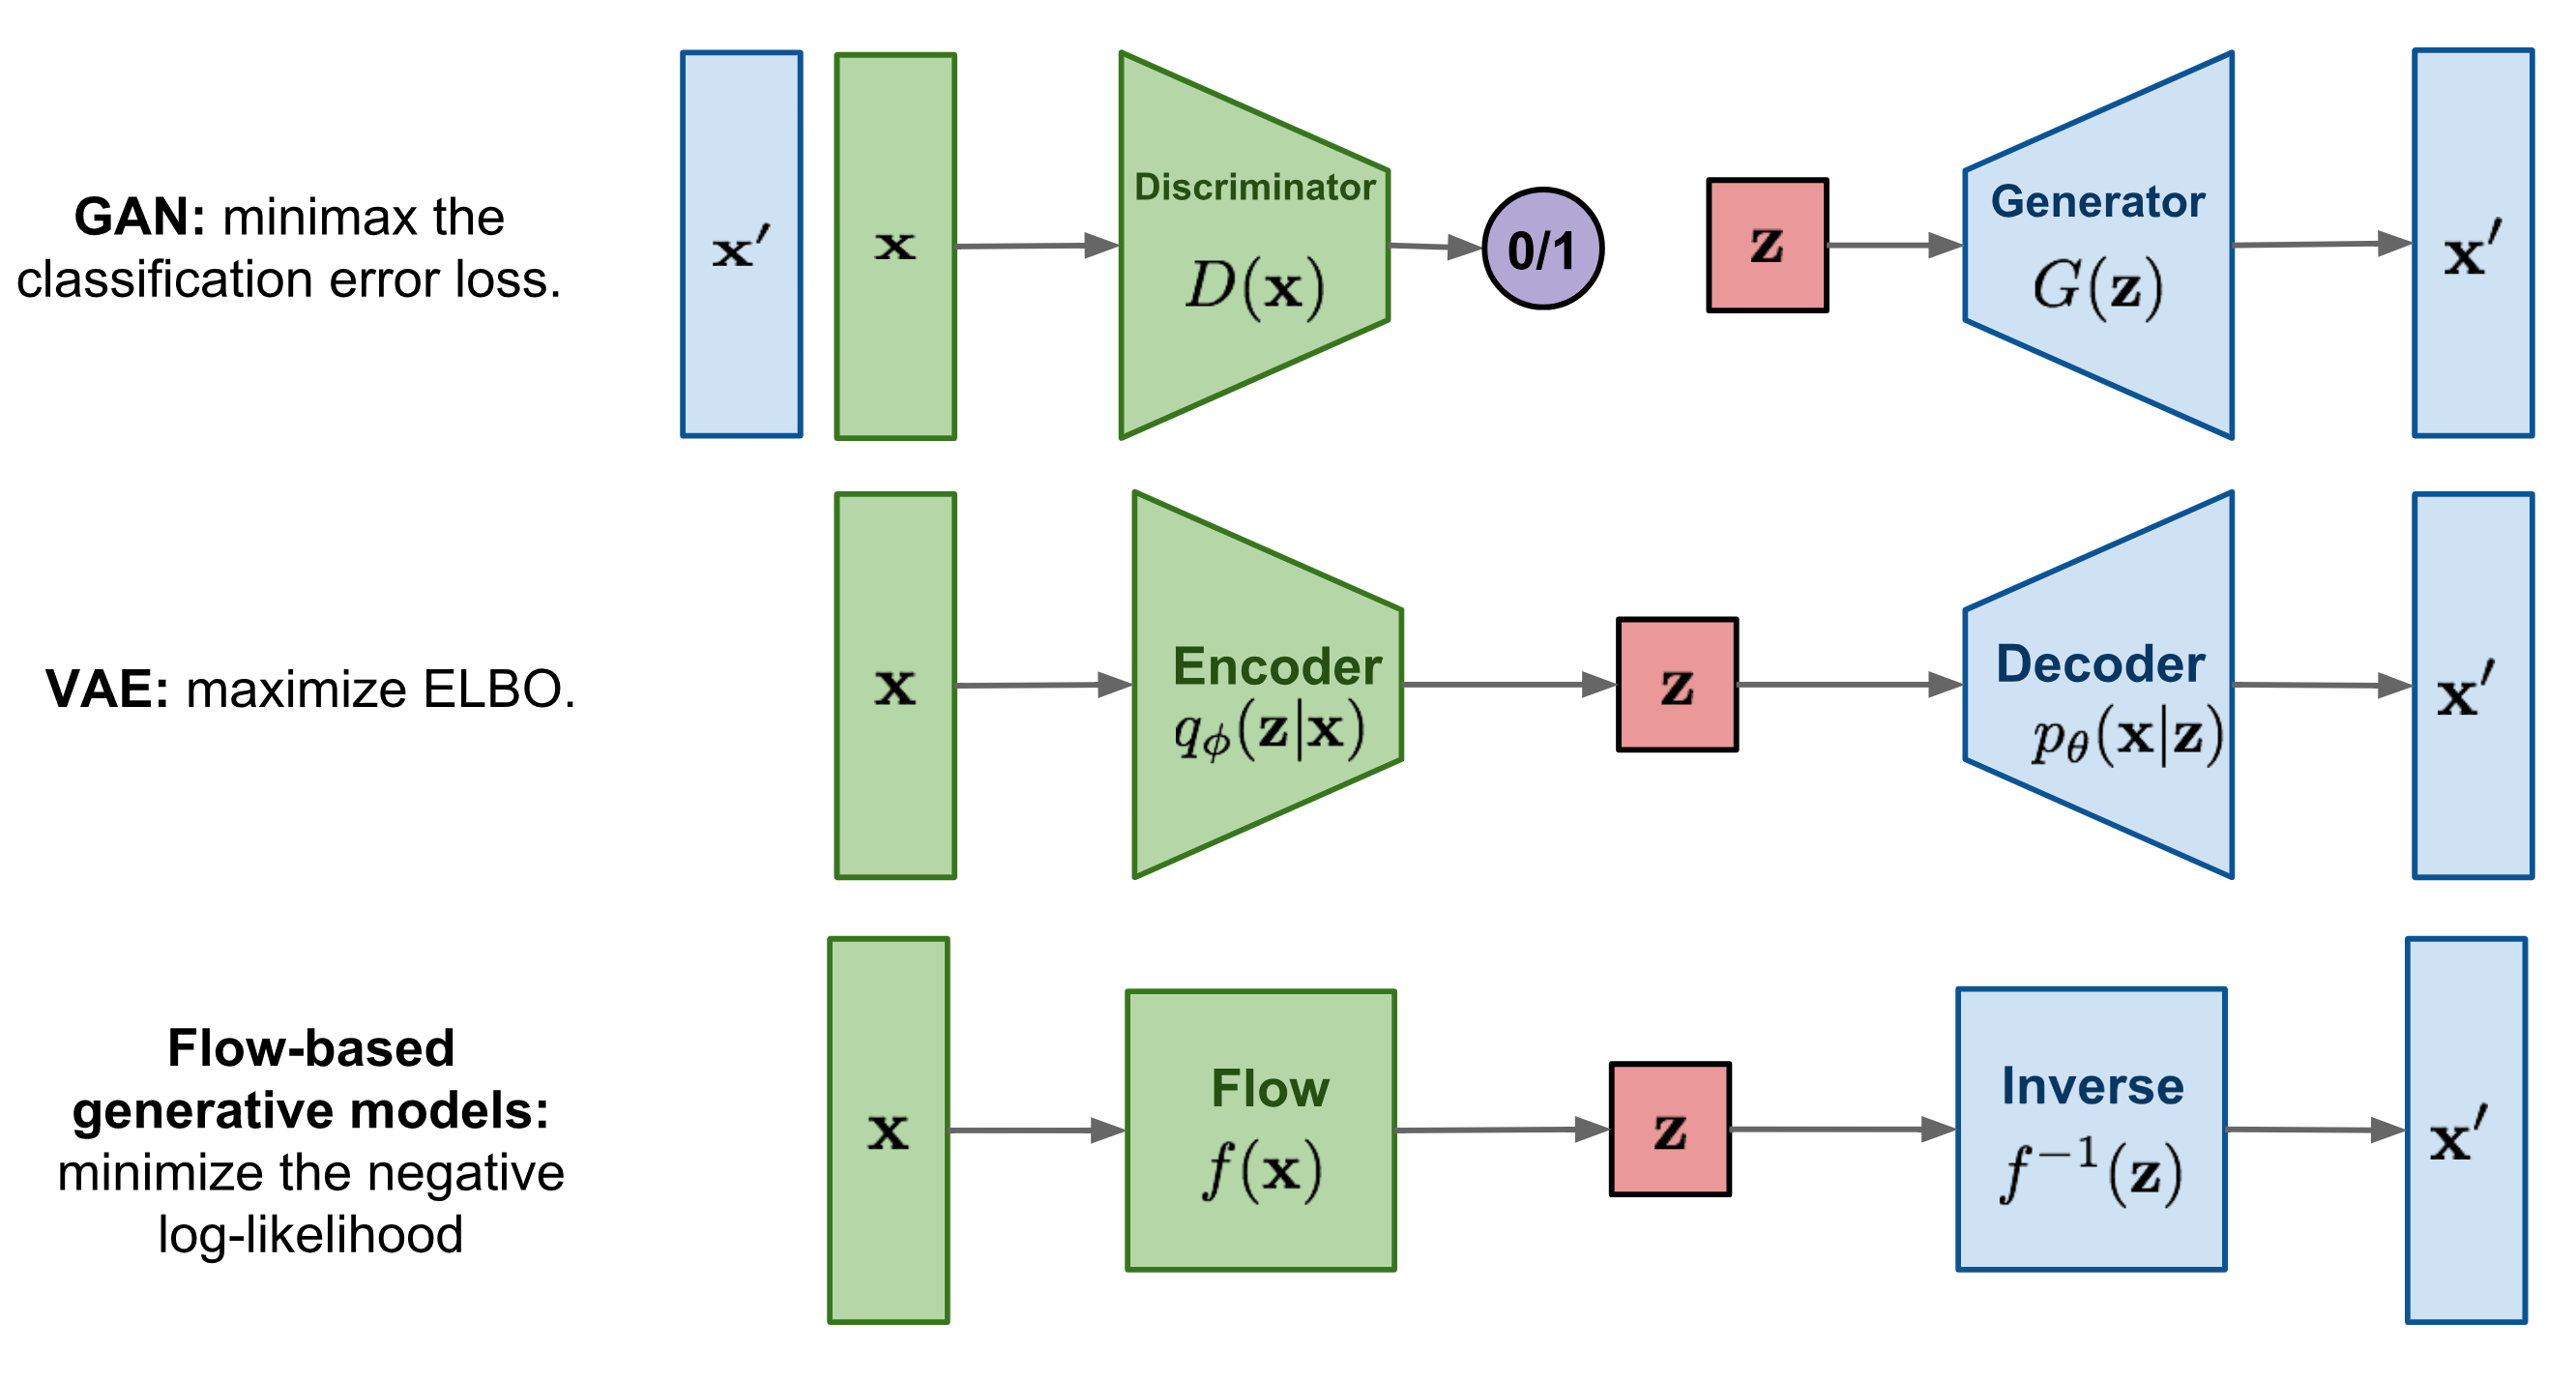
\includegraphics[scale=0.53]{./images/generative/flows/generative_models.png}
	\caption{An overview of generative models.}
\end{figure}

\begin{itemize}
	\item Flow-models get an exact estimate of the likelihood of your sample, as well as in the reverse direction. 
	\item VAEs optimize a lower bound on the (log) likelihood 
	\item GANs minimize a discrepancy between your input and transformed noise distributions. 
\end{itemize}



\section{The Method of Transformations of Random Variables}

If we are interested in finding the PDF of $Y=g(X)$, where $g(\cdot)$ is some deterministic transformation of $X$, and the function $g$ satisfies following properties, we can utilize a method called the method of transformations.
\begin{itemize}
	\item $g(x)$ is differentiable;
	\item $g(x)$ is a strictly (or monotonically) increasing function, that is, if $x_1<x_2$, then $g(x_1)<g(x_2)$.
\end{itemize}

% Now, let $X$ be a continuous random variable and $Y=g(X)$. We will show that you can directly find the PDF of $Y$ using the following formula.
% \begin{equation*}
% 	f_Y(y) = 
% 	\begin{cases}
% 	\frac{f_X(x_1)}{g'(x_1)}=f_X(x_1). \frac{dx_1}{dy} & \quad \textrm{where } g(x_1)=y\\
% 	0 & \quad \textrm{if }g(x)=y \textrm{ does not have a solution}
% 	\end{cases} 
% \end{equation*}

% Note that the derivative $\frac{dx}{dy}$ or $\frac{d}{dy}(g^{-1}(y))$ \textbf{measures how $X$ changes with respect to $Y$}.
% % Note that start with the function $y=f^{-1}(x)$. Write this as $x=f(y)$ and differentiate both sides implicitly with respect to$x$ using the Chain Rule:
% % \begin{align*}
% % 	1 &= f'(y)\frac{dy}{dx}\\
% % 	\frac{dy}{dx} &= \frac{1}{f'(y)}\\
% % 	y &= f^{-1}(x)\\
% % 	[f^{-1}]'(x) &= \frac{1}{f'(f^{-1}(x))}
% % \end{align*}
% Since $g$ is strictly increasing, its inverse function $g^{-1}$ is well defined. You can imagine a simple function like a linear function, \eg $Y=3X+1$. Then, for each $y\in R_Y$, there exists a \textbf{unique} $x_1$ such that $g(x_1)=y$. We can write $x_1=g^{-1}(y)$. Then,
% \begin{align*}
% 	\{Y\leq y\} = \{g(X)\leq y\} = \{X \leq g^{-1}(x)\}.
% \end{align*}
% Thus, 
% \begin{align*}
% 	F_Y(y) &= P(Y\leq y)\\
% 		   &= P(g(X)\leq y)\\
% 		   &= P(X\leq g^{-1}(y))\quad \text{, since }g \text{ is strictly increasing.}\\
% 		   &= F_X(g^{-1}(y)).
% \end{align*}
% To find the PDF of $Y$, we differentiate $F_Y(y)$ as follows:
% \begin{align*}
% 	f_Y(y) &= \frac{d}{dy}F_X(x_1)\quad \text{by } g(x_1)=y\\
% 		   &=\frac{dx_1}{dy}\cdot \underbrace{\frac{d}{dx_1}F_X(x_1)}_{=F'_X(x_1)}\\
% 		   &=\frac{dx_1}{dy}f_X(x_1)\\
% 		   &=f_X(g^{-1}(y))\left|\frac{d}{dy}(g^{-1}(y))\right|
% 		   % &= \frac{f_X(x_1)}{g'(x_1)} \quad \text{, since } \frac{dx}{dy}=\frac{1}{\frac{dy}{dx}}.
% \end{align*}
% We can repeat the same argument for the case where $g$ is \textbf{strictly decreasing}. In that case, $g'(x_1)$ will be \textbf{negative}, so we need to use $|g'(x_1)|$ . Thus, we can state the following theorem for a \textit{strictly monotonic function}. (A function $g:R\to R$ is called strictly monotonic if it is strictly increasing or strictly decreasing.)

% Actually, we assumed that $g$ was one-to-one out of convenience: the condition that $g$ is one-to-one is not necessary for change of variables to work: Consider a continuous random variable $X$ with domain $R_X$, and let $Y=g(X)$. Suppose that we can partition $R_X$ into a finite number of intervals such that $g(x)$ is strictly monotone and differentiable on each partition. Then the PDF of $Y$ is given by 
% \begin{align*}
% 	f_Y(y)= \sum_{i=1}^{n} \frac{f_X(x_i)}{|g'(x_i)|}= \sum_{i=1}^{n} f_X(x_i).
% 	\left|\frac{dx_i}{dy}\right|,
% \end{align*}
% where $x_1,\dots,x_n$ are real solutions to $g(x)=y$.

% \subsection{Intuitive Explanation}
How to derive the PDF of the random variable $Y=g(X)$ when one knows the PDF of the random variable $X$? If $X$ is discrete, we can derive the pmf for $Y$ by simply summing up the probability mass for all the $x$'s such that $f(x)=y$. For a general function $g$, there is no direct formula to get the PDF of the random variable $Y=g(X)$ knowing $p(X)$. There is a formula in case when $h$ is a differentiable one-to-one mapping from the range (\ie the support) of $X$ to the range of $Y$.

Take for example a random variable $X\sim \mathcal{N}(\mu, \sigma)$ and set $Y=\exp(X)$. The figure below shows some simulations of $X$ and the corresponding values of $Y$. The density of $X$ is shown in blue and the one of $Y$ is shown in orange in the vertical direction.

\begin{figure}[t]
	\centering
	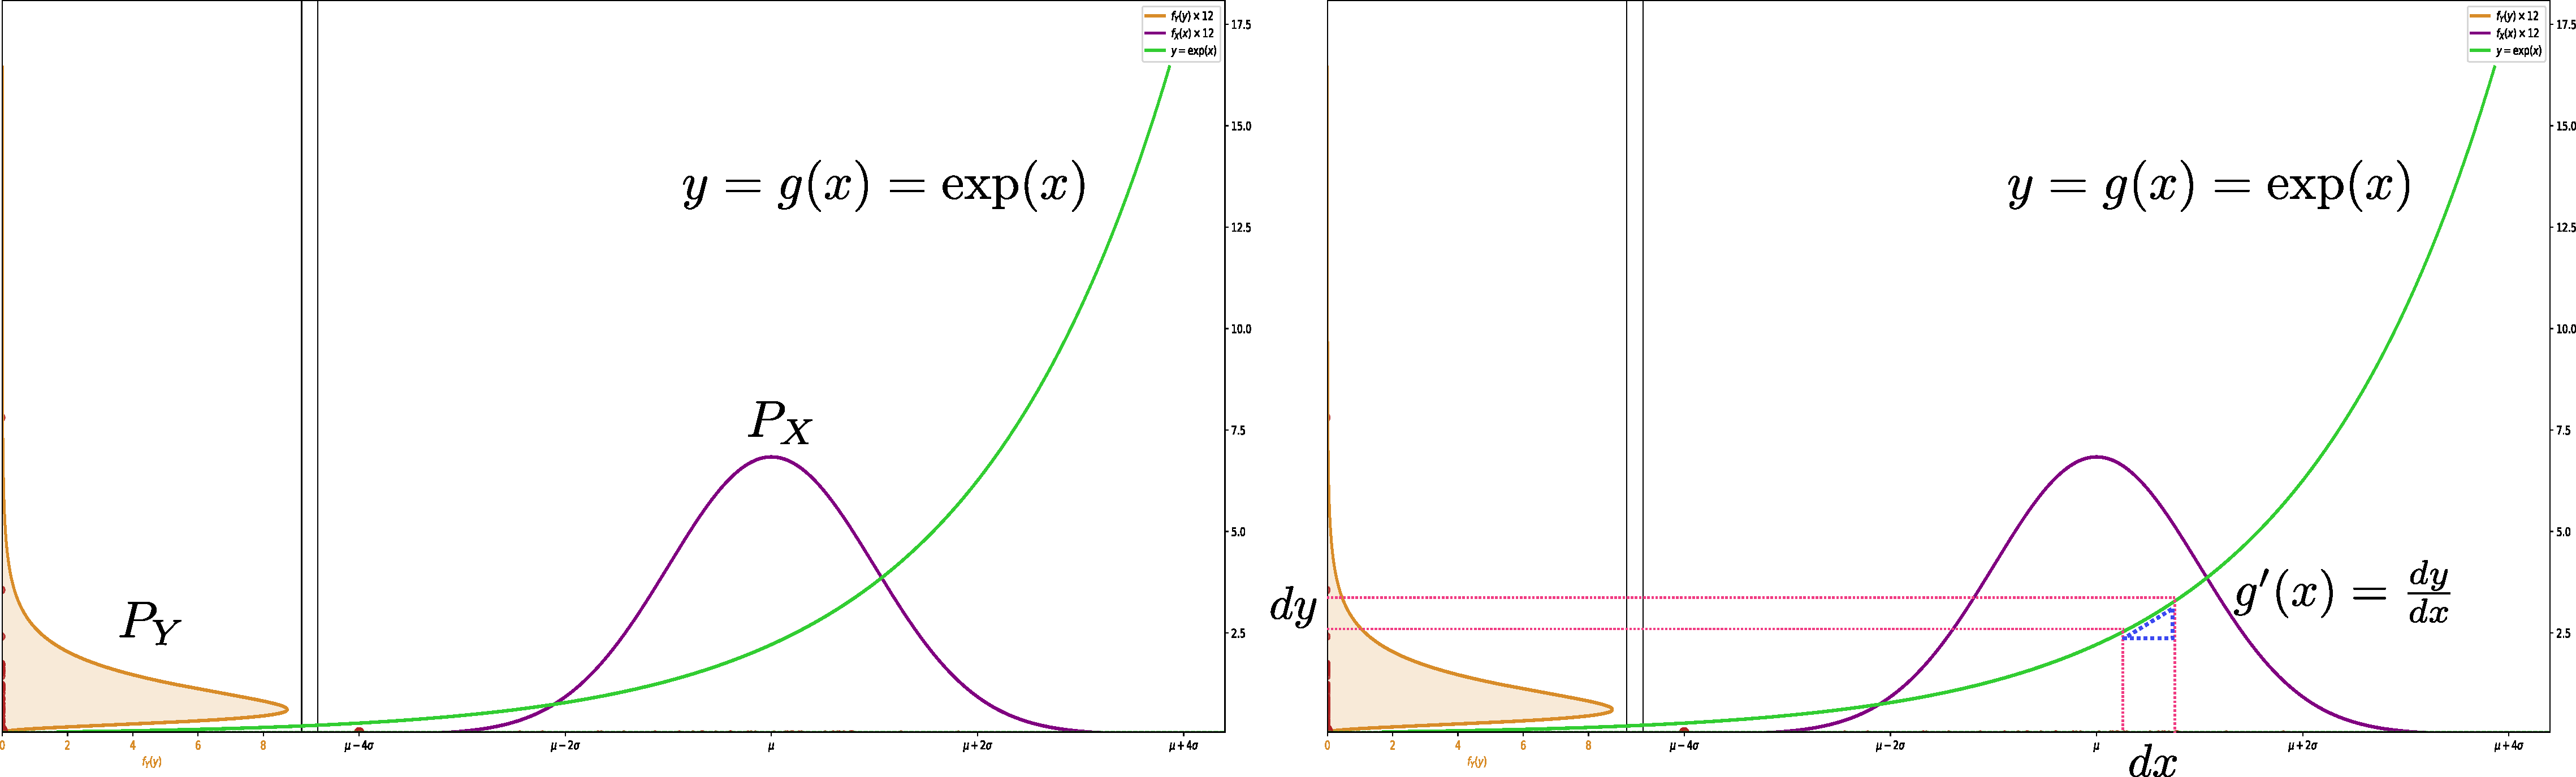
\includegraphics[scale=0.23]{./images/generative/flows/change_of_vars.pdf}
\end{figure}

\begin{figure}[t]
    \centering
    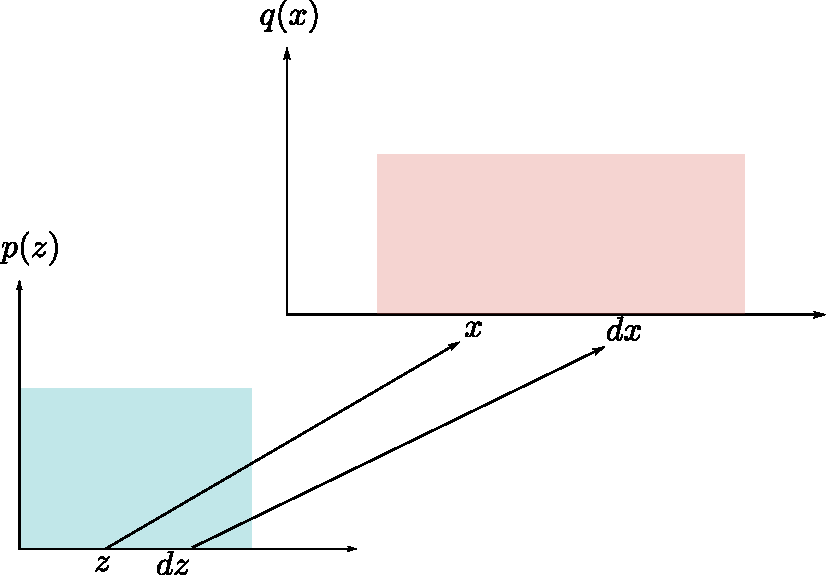
\includegraphics[scale=0.7]{./images/generative/flows/change_intuition.pdf}
    \caption{Area would be approximately $p(z)dz = q(z)dx$. Thus, $q(x) = p(z)\Big|\frac{dz}{dx}\Big|$}
    \label{fig:change_intuition}
\end{figure}


% \begin{figure}[ht]
%     \centering
%     \begin{minipage}[b]{0.45\textwidth}
%         \centering
%         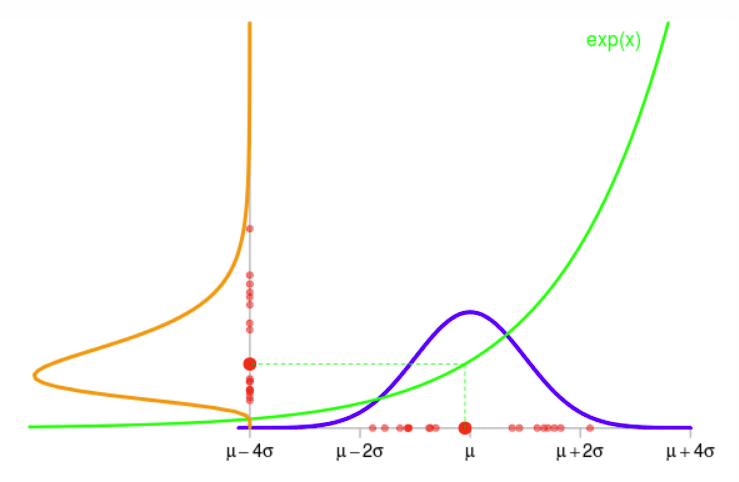
\includegraphics[width=\textwidth]{./images/generative/flows/sample.png}
%     \end{minipage}
%     \hfill
%     \begin{minipage}[b]{0.45\textwidth}
%         \centering
%         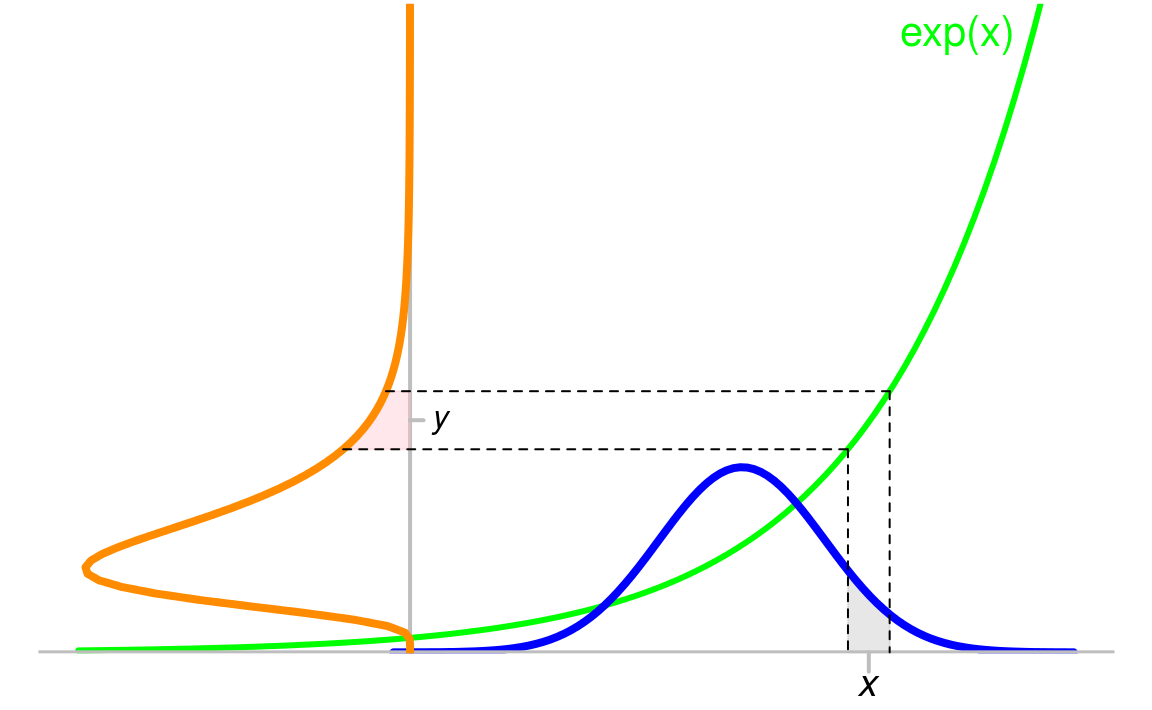
\includegraphics[width=\textwidth]{./images/generative/flows/sample2.png}
%     \end{minipage}
% \end{figure}
Now the question is: knowing the density of $X$, what is the density of $Y$?
Taking a point $y$ in the range of $Y$, the PDF $f_Y$ provides the probability of $Y$, belong to a small area $dy$ around $y$ by the formula below
$$P(Y\in dy)\approx f_Y(y)|dy|,$$
where $P(Y\in dy)$ is the area below the curve. Similarly, we can define
$$P(X\in dx)\approx f_X(x)|dx|$$
The above two areas are approximately the same in case of very small region. Note that if $dy$ and $dx$ are very small, we can approximate the derivative of $g'(x)=\frac{|dy|}{|dx|}$. Compactly, this can be expressed as follows:
$$P(X\in dx) = f_X(x)\frac{|dy|}{g'(x)}$$
With $y=g(x)$ we can get 
\begin{align*}
	P(X\in dx)\approx P(Y\in dy) &= f_X(x)\frac{|dy|}{g'(x)}\\
	& = f_X(g^{-1}(y))\frac{|dy|}{g'(g^{-1}(y))}\\
	& = f_X(g^{-1}(y))|dy|(g^{-1})'(y)
\end{align*}
The last line is by the derivative of inverse function which is 
\begin{align*}
	\frac{d}{dx}f^{-1}(x) = \frac{1}{f'(f^{-1}(x))}
\end{align*}
Then, 
\begin{align*}
	P(Y\in dy)\approx f_Y(y)|dy| = f_X(g^{-1}(y))|(g^{-1})'(y)|\cdot |dy|
\end{align*}
Finally, we can get 
$$f_Y(y) = f_X(g^{-1}(y))|(g^{-1})'(y)|$$
Note that the absolute is determined by the function $h$. This is the so-called \textit{change of variables formula}.



\subsection{Vector to Vector}

$Z$ and $X$ be random variables which are related by a mapping $f:\mathbb{R}^n\to \mathbb{R}^n$ such that $X=f(Z)$ and $Z=f^{-1}(X)$. Then
\begin{align*}
	p_X(\mathbf{x}) = p_Z(f^{-1}(\mathbf{x})) \left\vert \text{det}\left(\frac{\partial f^{-1}(\mathbf{x})}{\partial \mathbf{x}}\right) \right\vert
\end{align*}

Note that for any invertible square matrix $A$ over a field (\eg real or complex numbers),
\begin{align*}
	\det\bigl(A^{-1}\bigr)=\frac{1}{\det(A)}.
\end{align*}

Let
$$
A=\begin{bmatrix}
2 & 1\\[2pt]
3 & 4
\end{bmatrix}.
$$

Then, determinant of $A$ is given by
$$
\det(A)=2\cdot4-3\cdot1 = 8-3 = 5.
$$

The inverse of $A$ is 
$$
A^{-1}= \frac{1}{5}\begin{bmatrix}
4 & -1\\[2pt] -3 & 2
\end{bmatrix}.
$$

Then, the determinant of $A^{-1}$ is
$$
\det(A^{-1}) = \frac{1}{5^2}\bigl(4\cdot2-(-3)(-1)\bigr)
=\frac{1}{25}(8-3)=\frac{5}{25}=\frac{1}{5}.
$$

You can confirm the property:

$$
\det(A^{-1})=\frac{1}{5}=\frac{1}{\det(A)}.
$$


For example, we can transform $(x_1,x_2)$ to $(r,\theta)$ via $x_1=r\cos\theta$ and $x_2=r\sin\theta$.

Then
\[
J_{y\to x}=
\begin{pmatrix}
\dfrac{\partial x_1}{\partial r} & \dfrac{\partial x_1}{\partial\theta}\\[6pt]
\dfrac{\partial x_2}{\partial r} & \dfrac{\partial x_2}{\partial\theta}
\end{pmatrix}
=
\begin{pmatrix}
\cos\theta & -r\sin\theta\\
\sin\theta & \phantom{-}r\cos\theta
\end{pmatrix},
\tag{3}
\]
so
\[
\bigl|\det J_{y\to x}\bigr|
 = \bigl|\,r\cos^{2}\theta + r\sin^{2}\theta\,\bigr|
 = |r|.
\tag{4}
\]

Hence
\[
p_{\mathbf{y}}(\mathbf{y}) = p_{\mathbf{x}}(\mathbf{x})\,|J_{y\to x}|
\quad\Longrightarrow\quad
p_{R,\Theta}(r,\theta) = p_{X_1,X_2}(x_1,x_2)\,r.
\tag{5--6}
\]

For a two dimensional random vector $(X,Y)$ with density $p_{X,Y}$, 
\begin{align*}
	Pr((X,Y)\in A) = \int\int_A p_{X,Y}(x,y)dxdy.
\end{align*}
For a infinitesimally small region, we can approximate as follows:
\begin{align*}
	\int_x^{x+dx} p_{X}(x)dx \approx  p_{X}(x)dx.
\end{align*}

Similarly, we can get the probability as follows:
\[
P\!\bigl(r\le R\le r+dr,\;
        \theta\le\Theta\le\theta+d\theta\bigr)
  = p_{R,\Theta}(r,\theta)\,dr\,d\theta.
\tag{7}
\]
Note that the length of arc is $r\times d\theta$. Thus, the area $r\,dr\,d\theta$ or probability is given by
\[
P\!\bigl(r\le R\le r+dr,\;
        \theta\le\Theta\le\theta+d\theta\bigr)
  = p_{X,Y}(r\cos\theta, r\sin\theta)\,r\,dr\,d\theta,
\tag{8--9}
\]
so that finally
\[
p_{R,\Theta}(r,\theta)
  = p_{X,Y}(r\cos\theta, r\sin\theta)\,r.
\tag{10}
\]

% \begin{figure}[h]
%   \centering
%   % Replace the filename with the actual graphic if you have it.
%   \includegraphics[width=.55\linewidth]{polar_patch}
%   \caption{Change of variables from polar to Cartesian.
%            The area of the shaded patch is $r\,dr\,d\theta$.}
%   \label{fig:polarPatch}
% \end{figure}



\part{Natural Language Processing}
\chapter{Introduction}
\section{Evaluation Metrics}
\label{sec:nlp_eval_metrics}

\begin{itemize}
	\item Recall: TP/(TP+FN). Find all relevant cases whithin a dataset.
	\item Precision: TP/(TP+FP): While recall expresses the ability to find all relevant instances in a dataset, precision expresses the proportion of the data points our model says was relevant actually were relevant.
	\item The F1 score is the harmonic mean of precision and recall taking both metrics into account in the following equation:
\end{itemize}

\subsection{Perplexity}

Intuitively, perplexity can be understood as a \textit{measure of uncertainty}. The perplexity of a language model can be seen as the level of perplexity. Consider a language model with an entropy of three bits, in which each bit encodes two possible outcomes of equal probability. This means that when predicting a symbol, that language model has to choose among $2^3=8$ possible options. Thus, we can argue that this language model has a perplexity of 8.

It can be modeled as $2^H(P,Q)$:
\begin{align*}
	PPL(W) &= P(w_1,\cdots, w_N)^{-\frac{1}{N}}\\
	&\approx \Bigg(\prod_{i=1}^N P(w_i|w_{<i})\Bigg)^{-\frac{1}{N}}\\
	&= \sqrt[n]{\frac{1}{\prod_{i=1}^{N} P(w_{i}|w_{<i})}}
\end{align*}

Let's derive it from a cross-entropy. We want to optimize $P_\theta$ instead of the true distribution $P$:
\begin{align}
	% H & \approx -\sum_{i=1}^{N} \log P(w_{i}|w_{<i})\\
	\mathcal{L}_{CE} &= -\mathbb{E}_{w\sim P} [P_\theta(w_{i}|w_{<i})]\\
	&\approx -\frac{1}{N} \sum_{i=1}^{N} \log P_\theta(w_{i}|w_{<i})\\
	&= -\frac{1}{N} \log \prod_{i=1}^{N} P_\theta(w_{i}|w_{<i})\\
	&=  \log \Bigg(\prod_{i=1}^{N} P_\theta(w_{i}|w_{<i}) \Bigg)^{-\frac{1}{N}}\\
	&=  \log \sqrt[N]{\frac{1}{\prod_{i=1}^{N} P_\theta(w_{i}|w_{<i})}}\\
	\label{eq:ppl_entropy}
\end{align}
Thus, $PPL(W) = \exp\Big(\mathcal{L}_{CE}\Big).$

\subsection{Cross-Entropy and Perplexity}
\begin{align*}
	H(P,Q) &= -\sum_{x}P(x)\log Q(x) \\
	&= -\sum_{x}P(x) [\log P(x) + \log Q(x) - \log P(x)] \\
	&= -\sum_{x}P(x)\Bigg[\log P(x) + \log\frac{Q(x)}{P(x)}\Bigg] \\
	&= H(P) + D_{KL}(P||Q)
\end{align*}
It should be noted that since the empirical entropy $H(P)$ is unoptimizable, when we train a language model with the objective of minimizing the cross entropy loss, the true objective is to minimize the $KL$-divergence of the distribution, which was learned by our language model from the empirical distribution of the language.

\chapter{Classical NLP Techniques}

\section{Edit Distance}
\label{sec:nlp_edit_distance}

Edit distance is a method used in spell correction to determine how similar two words are by calculating the minimum number of operations (insertions, deletions, or substitutions) required to transform one word into another. The smaller the edit distance, the more similar the two words are.

For example, let's say we have the following dictionary of valid words: "cat", "car", "cart", "care", "cards", "cast". If the input word is "carr", we calculate the edit distance between "carr" and each word in the dictionary as follows:

\begin{itemize}
	\item cat: 3 (insert "r" and "r", then delete "t")
	\item car: 1 (replace second "r" with "t")
	\item cart: 2 (insert "t" and delete second "r")
\end{itemize}

The smallest edit distance is 1, between "carr" and "car", so "car" would be selected as the corrected word.

The edit distance method can be improved by using techniques such as weighting the importance of each operation (insertion, deletion, substitution) or using a more sophisticated algorithm such as \textit{Levenshtein distance}. Additionally, the method can be combined with other methods such as language modeling or phonetic analysis to further improve spell correction accuracy.

\section{Point-wise Mutual Information}
\label{sec:nlp_pmi}

Point-wise Mutual Information (PMI) is a statistical measure to calculate the association between two words in a given corpus. PMI is calculated by comparing the probability of the co-occurrence of two words with their individual probabilities of occurrence.

Formally, it is a quantity which is closely related to the mutual information is the point-wise mutual information. For two events (not random variables) $x$ and $y$, this is defined as
\begin{align}
	\textrm{PMI}[x,y] &\triangleq \textrm{log}\frac{p(x, y)}{p(x)p(y)}\\
					 &= \frac{p(x|y)}{p(x)}=\frac{p(y|x)}{p(y)}
	\label{eq:pmi}
\end{align}
This measures the discrepancy between these events occurring together compared to what would be expected by chance. 

\begin{itemize}
	\item $x$ and $y$ are two words being considered,
	\item $P(x)$ is the probability of the occurrence of word $x$ in the corpus,
	\item $P(y)$ is the probability of the occurrence of word $y$ in the corpus, and
	\item $P(x,y)$ is the probability of the co-occurrence of words $x$ and $y$ in the corpus. In other words, $x$ and $y$ are adjacent
\end{itemize}

For terms with three words, the formula becomes:
\begin{align*}
	\textrm{PMI}[x,y,z] &= \textrm{log}\frac{p(x, y, z)}{p(x)p(y)p(z)}
\end{align*}
PMI values can range from $-\infty$ to $\infty$. Positive PMI values indicate that the words have a strong association, while negative values indicate that the words are unlikely to appear together.

For example, consider a small corpus of text:
\begin{itemize}
	\item "The cat sat on the mat. The dog sat on the mat."
	\item The matrix below is $6\times 6$ considering all possible combination of the "forward" co-occurrences.
	\begin{align*}
		\begin{bmatrix}
		&the &cat &dog &sat &on  &mat\\
		the & 0  &1   &1   &0   &0   &2\\
		cat & 0  &0   &0   &1   &0   &0\\
		dog & 0  &0   &0   &1   &0   &0\\
		sat & 0  &0   &0   &0   &2   &0\\
		on  & 2  &0   &0   &0   &0   &0\\
		mat & 0  &0   &0   &0   &0   &0\\
		\end{bmatrix}
	\end{align*}
\end{itemize}


\subsection{Remove Stopwords prior to PMI}
In the above example we have not removed stopwords, so some of you might be wondering if we need to remove stopwords prior to PMI. It depends on the problem statement but if your objective is to find the related words, you should remove stopwords prior to calculating PMI. 

\section{TF-IDF}
\label{sec:nlp_tf_idf}

The term TF stands for term frequency, and the term IDF stands for inverse document frequency.

The TF-IDF representation takes into account the importance of each word in a document. In the bag-of-words model, each word is assumed to be equally important, which is obviously a less accurate assumption.

The method to calculate the TF-IDF weights of a term in a document is given by the following formula:

\begin{itemize}
	\item Term Frequency (TF), $tf(t,d)$, is the relative frequency of term t within document $d$,
		$$tf(t,d) = \frac{f_{t,d}}{\sum_{t'\in d}f_{t',d}},$$

		where $f_{t,d}$ is the raw count of a term in a document, \ie, the number of times that term $t$ occurs in document $d$. Note the denominator is simply the total number of terms in document $d$ (counting each occurrence of the same term separately). There are various other ways to define term frequency:
		\begin{itemize}
			\item The raw count itself: $tf(t,d) = f_{t,d}$ 
    		\item Boolean "frequencies": 
				\begin{align*}
					tf(t,d) = \begin{cases}
						1, \quad \text{if $t$ occurs in $d$}\\
						0 \quad \text{otherwise}
							\end{cases}
				\end{align*}
    		\item Logarithmically scaled frequency: $tf(t,d) = \log (1 + ft,d)$
    		\item Augmented frequency, to prevent a bias towards longer documents, \eg. raw frequency divided by the raw frequency of the most frequently occurring term in the document:
				\begin{align*}
					tf(t,d) = 0.5 + 0.5\frac{f_{t,d}}{\max \{f_{t',d}:t' \in d\}}
				\end{align*}
		\end{itemize}
	\item Inverse document frequency: The IDF is a measure of how much information the word provides, \ie, if it is common or rare across all documents. It is the logarithmically scaled inverse fraction of the documents that contain the word, which is obtained by dividing the total number of documents by the number of documents containing the term, and then taking the logarithm of that quotient: 
		\begin{align*}
			idf(t, D) = \log \frac{N}{|\{d\in D: t\in d\}|}
		\end{align*}
		\begin{itemize}
			\item $N$ total number of documents in the corpus ($=|D|$). 
			\item $|\{d\in D: t\in d\}|$: number of documents where the term $t$ appears. If the term is not in the corpus, this will lead to a division-by-zero. It is therefore common to adjust the numerator $1 + N$ and denominator to $1+|\{d\in D: t\in d\}|$.
			\item 
		\end{itemize}

\end{itemize}

\subsection{Term frequency–inverse document frequency}
TF-IDF is calculated as a multiplication of $tf(t, D)$ and $idf(t, D)$. 
\begin{itemize}
	\item A high weight in TF–IDF is reached by a high term frequency (in the given document) and a low document frequency of the term in the whole collection of documents; the weights hence tend to filter out common terms. 
	\item Since the ratio inside the IDF's log function is always greater than or equal to 1, the value of IDF (and TF–IDF) is greater than or equal to 0. 
	\item As a term appears in more documents, the ratio inside the logarithm approaches 1, bringing the IDF and TF–IDF closer to 0. 
\end{itemize}

% \subsection{Justification of IDF}
% Let's say
% \begin{align*}
% 	P(t|D) &= \frac{|\{d\in D: t\in d\}|}{N}.
% \end{align*}
% Then, 
% \begin{align*}
% 	IDF &= -\log P(t|D)\\
% 		&= \log \frac{1}{P(t|D)}\\
% 		&= \log \frac{N}{|\{d\in D: t\in d\}|}.\\
% \end{align*}

\subsection{Python Implementation}



\subsection{Link with Information Theory}
This expression shows that summing the TF–IDF of all possible terms and documents recovers the mutual information between documents and term taking into account all the specificities of their joint distribution. Each TF–IDF hence carries the "bit of information" attached to a term x document pair. 


\section{BM25}
\label{sec:nlp_bm25}











\section{Label Smoothing}
For each training example $x$, our model computes the probability of each label $k\in \{1,...,K\}$, $p(k|x) = \frac{\exp(z_k)}{\sum_i \exp(z_i)}$. Here $z_k$ are the logits.

Label smoothing is a mechanism to regularize the classifier layer by estimating the marginalized effect of label-dropout during training.

Vanila corss-entropy can cause two problem: 
\begin{itemize}
    \item First, it may result in over-fitting: if the model learns to assign full probability to the ground-truth label for each training example, it is not guaranteed to generalize. 
    \item Second, it encourages the differences between the largest logit and all others to become large, and this, combined with the bounded gradient $\frac{\partial \ell}{\partial z_k}$, reduces the ability of the model to adapt. Intuitively, this happens because the model becomes too confident about its predictions. 
\end{itemize}
We propose a mechanism for encouraging the model to be less confident. While this may not be desired if the goal is to maximize the log-likelihood of training labels, it does regularize the model and makes it more adaptable. The method is very simple. Consider a distribution over labels $u(k)$, independent of the training example $x$, and a smoothing parameter $\epsilon$. For a training example with ground-truth label $y$, we replace the label distribution $q(k|x) = \delta_{k,y}$ with
$$q'(k|x) = (1-\epsilon)\delta_{k,y}+\epsilon u(k)$$
which is a mixture of the original ground-truth distribution $q(k|x)$ and the fixed distribution $u(k)$, with weights $1-\epsilon$ and $\epsilon$, respectively. This can be seen as the distribution of the label $k$ obtained as follows: 
$$q'(k|x) = (1-\epsilon)\delta_{k,y}+\frac{\epsilon}{K} $$
We refer to this change in ground-truth label distribution as label-smoothing regularization, or LSR.

\subsection{\href{https://leimao.github.io/blog/Label-Smoothing/}{Another Interpretation}}

Instead of using one-hot encoded vector, we introduce noise distribution $u(y|x)$. Our new ground truth label for data $(x_i,y_i)$ would be

\begin{align*}
p^{\prime}(y|x_i) &= (1-\varepsilon) p(y|x_i) + \varepsilon u(y|x_i) \\
&=
\begin{cases}
    1 - \varepsilon + \varepsilon u(y|x_i) & \text{if } y = y_i \\
    \varepsilon u(y|x_i) & \text{otherwise}
\end{cases}
\end{align*}
Where $\varepsilon$ is a weight factor, $\varepsilon\in [0,1]$, and note that $\sum_{y=1}^{K}p'(y|x_i)=1$.

\chapter{POS Tagging}
\section{Introduction}
\label{sec:nlp_pos_intro}

Part-of-speech (POS) tagging is the process of labeling words in a text with their corresponding parts of speech in natural language processing (NLP). It helps algorithms understand the grammatical structure and meaning of a text.

\chapter{Transformer}
\section{Attention Mechanism}
\label{sec:nlp_attention}
The attention mechanism mimics the retrieval of a value $v_i$ for a query $q$ based on a key $k_i$ in database.
$$attn(q, k, v) = \sum_i sim(q,k_i)\times v_i$$
\begin{figure}[h]
	\centering
	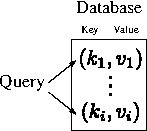
\includegraphics[scale=2.0]{./images/transformer/attention_database.pdf}
	\caption{The most similar key will be selected by measuring a similarity between a query and a key.}
\end{figure}

\begin{figure}[h]
	\centering
	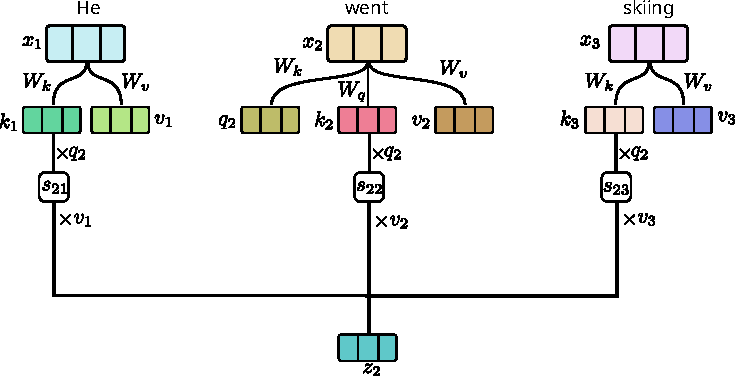
\includegraphics[scale=0.8]{./images/transformer/attention.pdf}
	\caption{The similarity $s_t$ is computed by a query and keys}
\end{figure}
There are several choices for a similarity function.
\begin{itemize}
	\item $q^Tk_i$: dot product.
	\item $\frac{q^Tk_i}{\sqrt{d}}$: scaled dot product.
	\item $q^TWk_i$: general dot product.
	\item $w_q^Tq+ w_k^Tk_i$: additive similarity.
\end{itemize}
Finally, the attention score can be computed by using a softmax:
$$a_i = \frac{\exp(s_i)}{\sum_j \exp(s_j)}$$

\section{Transformer}
\label{sec:nlp_transformer}

Attention:
$$attn(Q,K,V) = softmax(\frac{Q^TK}{\sqrt{d_k}})V$$
Masked attention:
$$\textrm{MA}(Q,K,V) = softmax\bigg(\frac{Q^TK+M}{\sqrt{d_k}}\bigg)V,$$
where $M$ is a matrix of 0 and $-\infty$. Note that $-\infty$ will make $exp$ term to be zero.




\part{Advanced Topics}
\chapter{Neural Ordinary Differential Equations}
\section{Preliminary}
\label{sec:node_preliminary}

\subsection{Euler Method}
The Euler method is a simple numerical technique used to solve ordinary differential equations (ODEs) of the form \( \frac{dy}{dt} = f(t, y) \). It is an initial value problem where we seek to find the function \( y(t) \) given an initial condition \( y(t_0) = y_0 \). Here's a step-by-step explanation of the Euler method:


\paragraph{Problem Setup:} Given,
\begin{itemize}
	\item A differential equation \( \frac{dy}{dt} = f(t, y) \)
	\item An initial condition \( y(t_0) = y_0 \)
\end{itemize}

\paragraph{Discretization:} The idea is to approximate the solution at discrete points. Let's denote:
\begin{itemize}
	\item \( t_n \) as the \( n \)-th time step
	\item \( y_n \) as the approximation of \( y(t_n) \)
\end{itemize}
We define a step size \( h \) such that \( t_{n+1} = t_n + h \).

\paragraph{Euler's Approximation:} Using the first-order Taylor series expansion, we can approximate \( y(t) \) at \( t_{n+1} \) as:
\[ y_{n+1} \approx y_n + h \cdot f(t_n, y_n) \]

\paragraph{Iterative Process:} Starting from the initial condition \( (t_0, y_0) \):
\begin{enumerate}
	\item Calculate the next value using the formula:
	\[ y_{n+1} = y_n + h \cdot f(t_n, y_n) \]
	\item Repeat the process for \( n = 0, 1, 2, \ldots \) until the desired value of \( t \) is reached.
\end{enumerate}

\paragraph{Example:} Let's solve the differential equation \( \frac{dy}{dt} = y \) with the initial condition \( y(0) = 1 \) using the Euler method.

\begin{itemize}
	\item Set the step size \( h \) (e.g., \( h = 0.1 \)).
	\item Start with \( t_0 = 0 \) and \( y_0 = 1 \).
\end{itemize}

Using the Euler formula:
\[ y_{1} = y_0 + h \cdot f(t_0, y_0) = 1 + 0.1 \cdot 1 = 1.1 \]
\[ y_{2} = y_1 + h \cdot f(t_1, y_1) = 1.1 + 0.1 \cdot 1.1 = 1.21 \]
\[ y_{3} = y_2 + h \cdot f(t_2, y_2) = 1.21 + 0.1 \cdot 1.21 = 1.331 \]

Euler's method can be visualized as taking small steps along the curve defined by the differential equation, using the slope at the current point to determine the direction of the next step.

\begin{figure}[h]
	\centering
	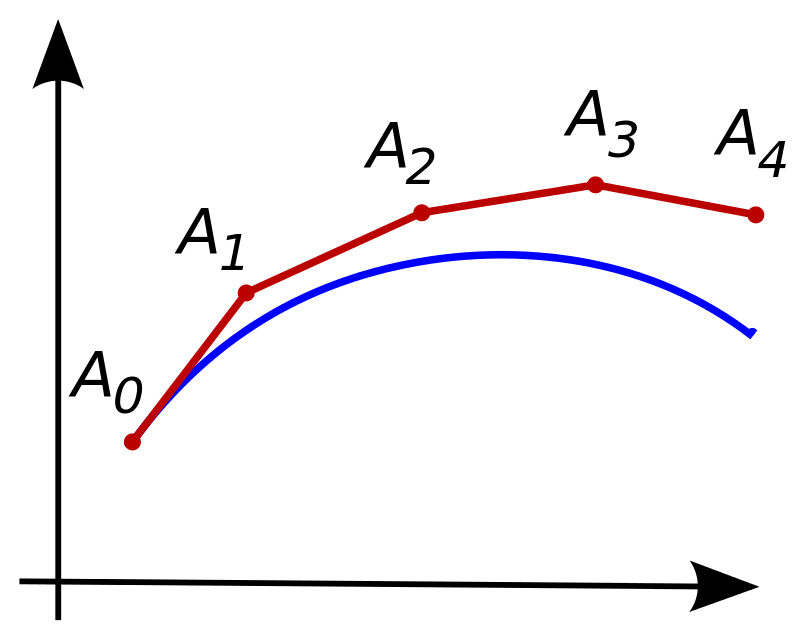
\includegraphics[scale=0.3]{./images/node/euler_method.png}
\end{figure}

\paragraph{Advantages:}
\begin{itemize}
	\item Simple to understand and implement.
	\item Requires only basic arithmetic operations.
\end{itemize}
\paragraph{Disadvantages:}
\begin{itemize}
	\item Low accuracy for large step sizes.
	\item Can become unstable if the step size is not chosen appropriately.
	\item Errors accumulate over time, leading to less accurate solutions.
\end{itemize}

Euler's method is often used as a basic introduction to numerical methods for solving ODEs, and more sophisticated methods like the \textit{Runge-Kutta} methods are used for more accurate solutions.



\section{Neural ODE}


Models such as residual networks, recurrent neural network decoders, and normalizing flows build complicated transformations by composing a sequence of transformations to a hidden state:
$$\rvh_{t+1} = \rvh_{t}+f(\rvh_{t}, \theta_t).$$

The $\rvh$ is iteratively updated as follows:
\begin{align*}
	\rvh_{2} &= \rvh_{1}+f(\rvh_{1}, \theta)\\
	\rvh_{3} &= \rvh_{2}+f(\rvh_{2}, \theta) = \rvh_{1}+f(\rvh_{1}, \theta)+f(\rvh_{2}, \theta)\\
	\vdots
\end{align*}
These iterative update can be seen as \textit{Euler discretization} of the \textit{continuous} transformation. Think of traditional neural networks as a sequence of steps. You give it some input, it goes through several steps (layers), and you get an output. Instead of thinking in steps, Neural ODEs think in \textbf{continuous change over time}. Note that this is the key contribution of this approach.   

Euler method can be expressed as follows: 
$$y_n = y_{n-1}+h\frac{\partial y_{n-1}}{\partial x_{n-1}},$$
where $h$ is the step size. In NODE, they view the $f$ as an ordinary differential equation, which depends on the state at time $t$ and parameter $\theta$. The following equation is the shape of Euler method:
$$y_n = y_{1}+h\frac{\partial y_{1}}{\partial x_{1}}+h\frac{\partial y_{2}}{\partial x_{2}}+\cdots+h\frac{\partial y_{n-1}}{\partial x_{n-1}}.$$
In NODE, 




\chapter{State Space Model}
\section{Introduction to State-Space Model}
\label{state:sec:ssm}
Reference: \href{http://apmonitor.com/pdc/index.php/Main/StateSpaceModel}{State-Space Models}.

The state of a dynamic system is a set of physical quantities, the specification of which completely determines the evolution of the system. The state variables are minimum set of variables that fully describe (enough information) the system. 

Many dynamic systems can be represented by using differential equations, since how the systems are changing is actually a function of current state. 
%For instance, if we want to depict a region, where its direction of wind varies by temperature and humidity. Then, we can set them as state variables. 
% \begin{figure}[h]
% 	\centering
% 	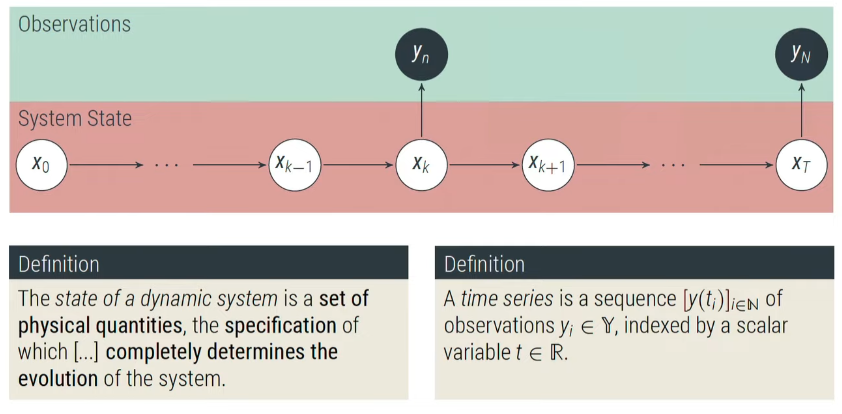
\includegraphics[scale=0.6]{./images/state_space/state_time_series.png}
% \end{figure}
% A probabilistic state-space model is a Bayesian model that defines
% \begin{itemize}
% 	\item An initial distribution $\rvx_0\sim p(\rvx_0)$ as a prior over the very first state, and for the state $\rvx_k\in \mathbb{R}^D$ and measurement $\rvy_k\in\mathbb{R}^d$ at time step $k$.
% 	\item A dynamics model as the prior over the (forward) state transitions.
% 		$$\rvx_k\sim p(\rvx_k|\rvx_{k-1}), $$
% 	\item A measurement model is a generative model for observations of the latent state.
% 		$$\rvy_k\sim p(\rvy_k|\rvx_{k}), $$
% \end{itemize}
\begin{align*}
	\dot{x} &= {A}x+{B}u,\\
	% \frac{dX}{dt} &= {A}X+{B}U,\\
	y &= {C}x+Du.
\end{align*}
The first and the second equations are known as \textit{state equation} and \textit{output equation}, respectively. The state equation tells us that how the state vector changes with the state vector and the (external) input. 

\begin{itemize}
	\item $x\in \mathbb{R}^n$: A state vector.
	\item $\dot{x}\in \mathbb{R}^n$: state derivative \ie $\big(\frac{dX}{dt}\big)$ represents the changes of the state vector. You can notice that this is a linear combination of state vector and the input vector. 
	\item $u\in \mathbb{R}^m$: Input
	\item $y\in \mathbb{R}^p$: Output
	\item $A\in \mathbb{R}^{n\times n}$: This matrix describes how the state vector influences the changes of the state vector. 
	\item $B\in \mathbb{R}^{n\times m}$: This matrix describes how the (external) input vector influences the changes of the state vector. 
	\item $C\in \mathbb{R}^{p\times n}$: Typically, an identity matrix ($I$).
	\item $D\in \mathbb{R}^{p\times m}$: Typically, zeros
\end{itemize}


\subsection{Stability}

The linear state space model is stable if all eigenvalues of $A$ are negative real numbers or have negative real parts to complex number eigenvalues. If all real parts of the eigenvalues are negative then the system is stable, meaning that any initial condition converges exponentially to a stable attracting point. If any real parts are zero then the system will not converge to a point and if the eigenvalues are positive the system is unstable and will exponentially diverge.

\subsection{First Order System in State Space}

Let's consider an example to transform a first order linear system (without time delay):
\begin{align*}
	\tau_{p}\frac{dy}{dt} &= -y+K_pu,\\
\end{align*}
where $\tau_{p}$ and $K_p$ are time constant and gain, respectively. Then, we can transform it into a state space form as follows:
\begin{align*}
	\dot{x}&= \bigg[-\frac{1}{\tau_p}\bigg]x+\bigg[\frac{K_p}{\tau_p}\bigg]u,\\
	y &= [1]x+[0]u\\
	  &= x.
\end{align*}
Here, $A=-\frac{1}{\tau_p}$, $B = \frac{K_p}{\tau_p}$, $C=1$, and $D=0$. We can solve such model by using various methods like Laplace transform. 


% If the eigenvalues of $A$ are all smaller than $0$, then the system is called \textit{stable}. 

% \begin{itemize}
% 	\item $X\in \mathbb{R}^n$ and ${dX}/{dt}$ are the state vector and the differential state vector, respectively. 
% 	\item $U$ and $Y$ are scalar input vector and scalar output vector, respectively. 
% 	\item $A$ is the system matrix.
% 	\item $B$ and $C$ are the input and the output matrices.
% 	\item $D$ is the feed-forward matrix.
% \end{itemize}


\section{Efficiently Modeling Long Sequences with Structured State-Spaces}
\label{sec:}
The state space model (SSM) can be defined as follows:
\begin{align*}
	x'(t) &= \mathbf{A}x(t)+\mathbf{B}u(t),\\
	y(t) &= \mathbf{C}x(t)+\mathbf{D}u(t).
\end{align*}

It maps a single dimensional input signal $u(t)$ to an $N$-dim latent state $x(t)$ before projecting to a one-dim output signal $y(t)$.  

Our goal is to simply use the SSM as a black-box representation in a deep sequence model, where $\rmA, \rmB, \rmC$, and $\rmD$ are parameters learned by gradient descent. We will omit the parameter $\rmD$ for exposition (or equivalently, assume $\rmD=0$, because the term $\rmD u$ can be viewed as a skip connection and is easy to compute).

An SSM maps a input $u(t)$ to a state representation vector $x(t)$ and an output $y(t)$. For simplicity, we assume the input and output are one-dimensional, and the state representation is $N$-dimensional. The first equation defines the change in $x(t)$ over time.

% \begin{lstlisting}[language=Python]
% 	def random_SSM(rng, N):
% 		a_r, b_r, c_r = jax.random.split(rng, 3)
% 		A = jax.random.uniform(a_r, (N, N))
% 		B = jax.random.uniform(b_r, (N, 1))
% 		C = jax.random.uniform(c_r, (1, N))
%     return A, B, C
% \end{lstlisting}



\chapter{DeepSeek}

\section{Multi-Head Latent Attention}

\begin{figure}[h]
	\centering
	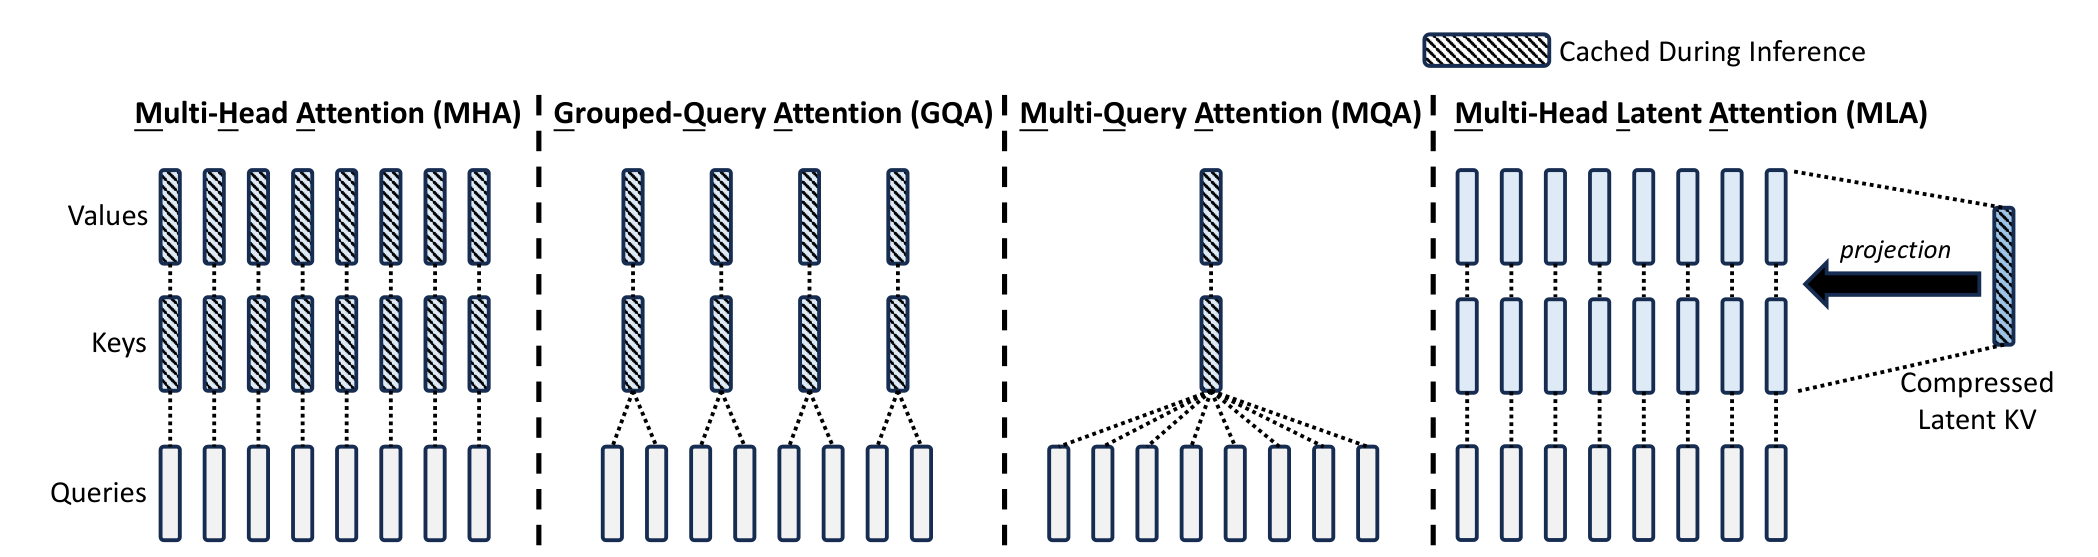
\includegraphics[scale=0.32]{./images/transformer/mla.png}
\end{figure}

The query, key, and value of the vanilla multi-head attention can be expressed as follows:
\begin{align*}
	\rvq_t &= W^{Q}\rvh_t\\
	\rvk_t &= W^{K}\rvh_t\\
	\rvv_t &= W^{V}\rvh_t
\end{align*}
\begin{itemize}
	\item $\rvq_t,\rvk_t,\rvv_t\in \mathbb{R}^{d_hn_h}$
	\item $\rvh_t\in \mathbb{R}^{d}$: Attention input of the $t$-th token at an layer.
	\item $d_h$: the attention head's dimension
	\item $n_h$: the number of attention heads
\end{itemize}
During inference, all keys and values need to be cached to accelerate inference, so MHA needs to cache $2n_hd_hl$ elements (\ie key, value for each layer and head) for each token. In model deployment, this heavy KV cache is a large bottleneck that limits the maximum batch size and sequence length.


\begin{figure}[h]
	\centering
	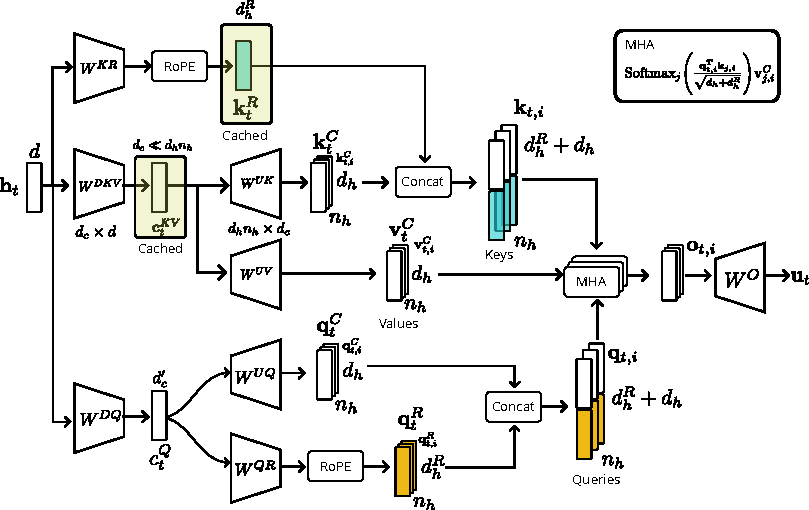
\includegraphics[scale=1.1]{./images/transformer/mla.pdf}
	\caption{The overview of MLA}
\end{figure}
The core of Multi-Head Latent Attention (MLA) is the low-rank joint compression for attention keys and values to reduce Key-Value (KV) cache during inference:
\begin{align*}
	\rvc_t^{KV} &= W^{DKV}\rvh_t\\
	[\rvk_{t,1}^C; \rvk_{t,2}^C; \dots ;\rvk_{t,n_h}^C;] = \rvk_t^{C} &= W^{UK}\rvc_t^{KV}\\
	\rvk_t^{R} &= \text{RoPE}(W^{KR}\rvh_t)\\
	\rvk_{t,i} &= [\rvk_{t,i}^C;\rvk_t^{R}]\\
	[\rvv_{t,1}^C; \rvv_{t,2}^C; \dots ;\rvv_{t,n_h}^C;] = \rvv_t^{C} &= W^{UV}\rvc_t^{KV}
\end{align*}
\begin{itemize}
	\item $\rvc_t^{KV}\in \mathbb{R}^{d_c}$ is the compressed \textit{latent vector} for keys and values, where $d_c\ll d_hn_h$. \textbf{Note that this is not a query vector.}
	\item $W^{DKV}\in \mathbb{R}^{d_c\times d}$ is the down-projection matrix
	\item $W^{UK},W^{UV}\in \mathbb{R}^{d_hn_h\times d_c}$ are the up-projection matrices for keys and values, respectively.
	\item $W^{KR}\in \mathbb{R}^{d_h^R\times d}$ is the matrix used for generating the decoupled key of RoPE. 
	\item \textbf{During inference, MLA only needs to cache $\rvc_t^{KV}$ and $\rvk_t^{R}$, which is a compressed latent vector, rather than high-dimensional key and value vector.} Thus, it can still have the multiple heads. This alleviates the issue of GQA or MQA while keeping their benefits. 
	% \item Thus, KV cache has only $d_c\times l$ elements, where $l$ is the number of layers.
	% \item Note that during inference the up-projection matrices W^UK and W^UV can be absorbed (Associative law of matrix multiplication) into the query(W^Q) and output(W^O) projections matrices, eliminating the need to compute keys and values explicitly.
\end{itemize}
% Unlike the MHA, MLA only needs to keep the $\rvc_t^{KV}$ and $\rvk_t^{R}$ (\ie cache). This leads to a significant memory usage. It does not look very clear at first. Let's closely look at the inner product of $\rvq$ and $\rvk$:
% \begin{align*}
% 	\rvq_t^T\rvk_t = \rvc_t^Q(W^{UQ}W^{UK})\rvc_T^{KV}
% \end{align*}
% \begin{itemize}
% 	\item As you can see the query and the key projected from the weight matrices allow them to be defined specifically in advance. 
% \end{itemize}

Moreover, in order to reduce the activation memory during training, we also perform low-rank compression for the queries, even if it cannot reduce the KV cache:
\begin{align*}
	\rvc_t^{Q} &= W^{DQ}\rvh_t\\
	[\rvq_{t,1}^C; \rvq_{t,2}^C; \dots ;\rvq_{t,n_h}^C;] = \rvq_t^{C} &= W^{UQ}\rvc_t^{Q}\\
	[\rvq_{t,1}^R; \rvq_{t,2}^R; \dots ;\rvq_{t,n_h}^R;] = \rvq_t^{R} &= \text{RoPE}(W^{QR}\rvc_t^Q)\\
	\rvq_{t,i} &= [\rvq_{t,i}^C;\rvq_{t,i}^{R}]
\end{align*}
\begin{itemize}
	\item $\rvc_t^{Q}\in \mathbb{R}^{d_c'}$ is the compressed latent vector for queries, where $d_c'\ll d_hn_h$
	\item $W^{DQ}\in \mathbb{R}^{d_c'\times d}$ and $W^{UQ}\in \mathbb{R}^{d_hn_h\times d_c'}$ are the down- and up- projection matrices for queries, respectively.
	\item $W^{QR}\in \mathbb{R}^{d_h^Rn_h\times d_c'}$ is the matrix for decoupled queries of RoPE.
\end{itemize}

Finally, the attention queries ($\rvq_{t,i}$), keys ($\rvk_{j,i}$), and values ($\rvv_{j,i}^C$) are combined to yield the final attention output $\rvu_t$:
\begin{align*}
	\rvo_{t,i} &= \sum_{j=1}^t\text{Softmax}_j\Bigg( \frac{\rvq_{t,i}^T\rvk_{j,i}}{\sqrt{d_h+d_h^R}} \Bigg)\rvv_{j,i}^C,\\
	\rvu_t &= W^O[\rvo_{t,1};\rvo_{t,2};\dots;\rvo_{t,n_h}],
\end{align*}
where $W^O\in \mathbb{R}^{d\times d_hn_h}$ is the output projection matrix.


\section{DeepSeek MoE}

This paper mentioned that the conventional TopK MoE has Knowledge Hybridity and Knowledge Redundancy. Knowledge Hybridity: existing MoE practices often employ a limited number of experts (e.g., 8 or 16), and thus tokens assigned to a specific expert will be likely to cover diverse knowledge. Consequently, the designated expert will intend to assemble vastly different types of knowledge in its parameters, which are hard to utilize simultaneously. (2) Knowledge Redundancy: tokens assigned to different experts may require common knowledge. As a result, multiple experts may converge in acquiring shared knowledge in their respective parameters, thereby leading to redundancy in expert parameters. These issues collectively hinder the expert specialization in existing MoE practices, preventing them from reaching the theoretical upper-bound performance of MoE models. By finely segmenting to more experts and introducing shared experts, DeepSeekMoE mitigated above tow issues.


\begin{figure}[t]
	\centering
	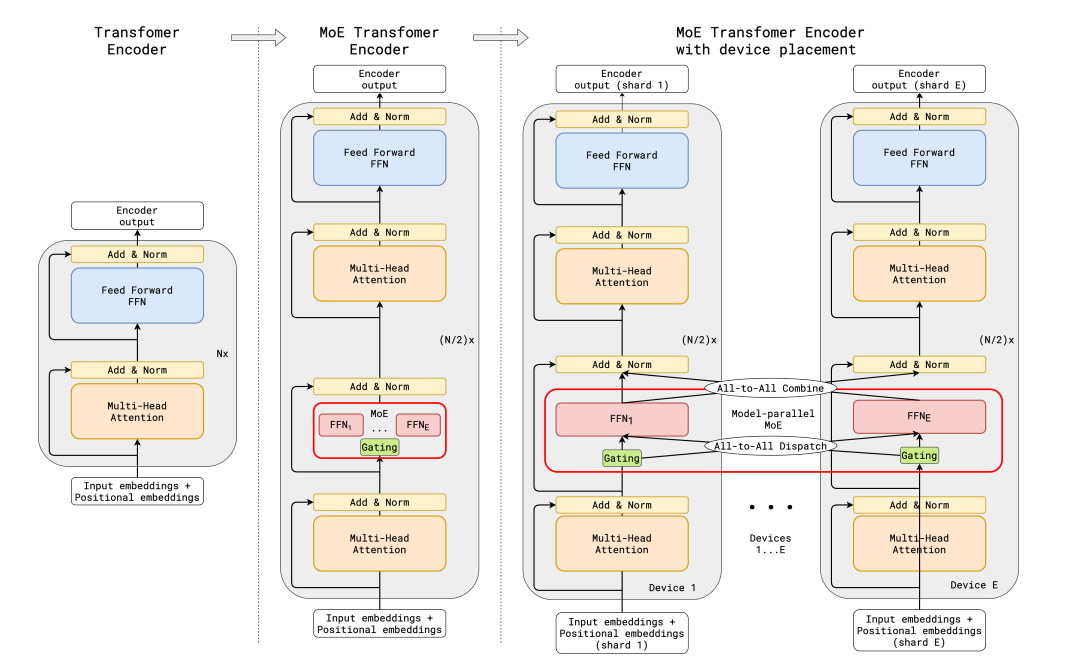
\includegraphics[scale=0.35]{./images/transformer/moe_block.png}
	\caption{MoE Transformer Encoder from the GShard Paper}
\end{figure}
A typical practice to construct an MoE language model usually substitutes FFNs in a Transformer with MoE layers at specified intervals. An MoE layer is composed of multiple experts, where each expert is structurally identical to a standard FFN. Then, each token will be assigned to one or two experts. If the 𝑙-th FFN is substituted with an MoE layer, the computation for its output hidden state h𝑙 𝑡is expressed as:


\begin{align*}
	\rvh_t' = \rvu_t+\sum^{N_s}_{i=1}FFN_i^{(s)}(\rvu_t)+\sum^{N_r}_{i=1}g_{i,t}FFN_i^{(r)}(\rvu_t),
\end{align*}
\begin{itemize}
	\item 
		$$g_{i,t} = \frac{g_{i,t}'}{\sum^{N_r}_{j=1}g_{j,t}'}$$
	\item 
		\begin{align*}
			g_{i,t}' = \begin{cases}
				s_{i,t}&\text{ } s_{i,t}\in TopK(\{s_{j,t}|1\leq j \leq N_r\}, K_r)\\
				0&\text{otherwise,}
			\end{cases}
		\end{align*}
	\item 
		$$s_{i,t} = \sigma(\rvu_t^T\rve_i)$$
	\item $\rvu_t$: FFN input of the $t$-th token. 
	\item $\rvh_t'$ FFN output
	\item $N_s$ and $N_r$ are the number of \textit{shared} experts and the \textit{routed} experts, respectively.
	\item $FFN_i^{(s)}(\cdot)$ and $FFN_i^{(r)}(\cdot)$ are the $i$-th \textit{shared} expert and the $i$-th \textit{routed} expert, respectively.
		\begin{itemize}
			\item The shared experts are always activated, aiming at capturing and consolidating common knowledge across varying contexts. 
			\item Through compressing common knowledge into these shared experts, redundancy among other routed experts will be mitigated.
		\end{itemize}
	\item $K_r$ is the number of activated routed experts
	\item $g_{i,t}$: gating value for the $i$-th expert, which is sparse by its nature. 
	\item $s_{i,t}$: a token assigned to an expert (\ie affinity score)
	\item $\rve_i$: the centroid vector of the $i$-th (routed) expert 
		\begin{itemize}
			\item This is an (learnable) expert embedding. 
		\end{itemize}
	\item $TopK(\cdot, K)$: the set comprising $K$ highest scores among the affinity scores calculated for the $t$-th token and all routed experts.
	\item $\sigma$: Sigmoid function.
\end{itemize}

Let's closely look at the equation
\begin{align*}
	\rvh_t' = \rvu_t+\sum^{N_s}_{i=1}FFN_i^{(s)}(\rvu_t)+\sum^{N_r}_{i=1}g_{i,t}FFN_i^{(r)}(\rvu_t),
\end{align*}
\begin{itemize}
	\item $\rvu_t+\dots$: this is just a skip connection
	\item $\sum^{N_s}_{i=1}FFN_i^{(s)}(\rvu_t)$: Always activated
	\item $\sum^{N_r}_{i=1}g_{i,t}FFN_i^{(r)}(\rvu_t)$
		\begin{itemize}
			\item Here, we can notice that $g_{i,t}$ is the weight for the corresponding (routed) experts
		\end{itemize}
\end{itemize}

To balance the load of the experts, DeepSeek also introduces a bias term $b_i$ for each expert and add it to the corresponding scores $s_{i,t}$ as follows:
\begin{align*}
	g_{i,t}' = \begin{cases}
		s_{i,t}&\text{ } s_{i,t}+b_i\in TopK(\{s_{j,t}+b_i|1\leq j \leq N_r\}, K_r)\\
		0&\text{otherwise,}
	\end{cases}
\end{align*}
During training, the bias term decreases by $\gamma$ at the end of each step if its corresponding expert is overloaded. 


\section{Multi-Token Prediction}

DeepSeek also adopts a multi-token prediction approach and they show that it can improve the output quality and generalization behaviors. One of potential reasons would be that MTP may mitigate the distributional discrepancy between training time teacher forcing and inference time autoregressive generation.

Unlike the conventional MTP approach, they keep the complete causal chain at each prediction depth by introducing MTP modules.

The input tokens $[t_1,t_2,t_3,t_4]$ go through the main model's transformer blocks and then go through the output head of main model to produce next predicted token $t_5$. Meanwhile the representation of the input tokens $[t_1,t_2,t_3,t_4]$ (\ie output of main model's transformer blocks) will be passed to the MTP module and combine them with new input tokens' embedding$[t_2,t_3,t_4,t_5]$ to help produce additional token $t_6$. In DeepSeek-V3, the model is designed to predict next 2 tokens.

\begin{align*}
	\rvh_i^{'k} = M_k[\text{RMSNorm}(\rvh_i^{k-1}); \text{RMSNorm}(\text{Emb}(t_{i+k}))]
\end{align*}
\begin{itemize}
	\item $\rvh_i^{k-1}$: $i$-th token at the $(k-1)$-th depth 
	\item $(i+k)$-th token embedding $\text{Emb}(t_{i+k})$
\end{itemize}

% \section{Decoupled RoPE}

\section{Reinforcement Learning}

\section{Training FrameWork}
\begin{itemize}
	\item 2048 H800 GPUs
	\item HAI-LLM framework: their custom framework. 
	\item 16-way Pipeline Parallelism
		\begin{itemize}
			\item The layers of a model are sharded across multiple devices. 
		\end{itemize}
	\item Expert Parallelism: evenly distributes some of the experts' full weight to different GPUs, which means each GPU holds part of the experts' full weight. \eg experts 1, 2, and 3 are assigned to the first GPU, while experts 4, 5, and 6 are assigned to the second one.
	\item ZeRO-1 DP
\end{itemize}
\section{DualPipe}
\section{FP8}





\part{Appendix}
\renewcommand{\thesection}{\Alph{section}.\arabic{section}}
\setcounter{section}{0}

\begin{appendices}
\chapter{Appendix}

\section{KL Divergence between Two Normal Distribution}
\begin{align*}
D_\text{KL}(P||Q) & = \mathbb{E}_P\Big[\textrm{log}\frac{P}{Q}\Big]\\
\end{align*}
Consider two multivariate Gaussians in $\mathbb{R}^n$, $P_1$ and $P_2$

\begin{align*}
D_\text{KL}(P||Q) &= \int \left[ \frac{1}{2} \log\frac{|\Sigma_2|}{|\Sigma_1|} - \frac{1}{2} (x-\mu_1)^T\Sigma_1^{-1}(x-\mu_1) + \frac{1}{2} (x-\mu_2)^T\Sigma_2^{-1}(x-\mu_2) \right] \times p(x) dx \\
&= \frac{1}{2} \log\frac{|\Sigma_2|}{|\Sigma_1|} - \frac{1}{2} \text{tr} \left\{E[(x - \mu_1)(x - \mu_1)^T] \ \Sigma_1^{-1} \right\} + \frac{1}{2} E[(x - \mu_2)^T \Sigma_2^{-1} (x - \mu_2)] \\
&= \frac{1}{2} \log\frac{|\Sigma_2|}{|\Sigma_1|} - \frac{1}{2} \text{tr}\ \{I_n \} + \frac{1}{2} (\mu_1 - \mu_2)^T \Sigma_2^{-1} (\mu_1 - \mu_2) + \frac{1}{2} \text{tr} \{ \Sigma_2^{-1} \Sigma_1 \} \\
&= \frac{1}{2}\left[\log\frac{|\Sigma_2|}{|\Sigma_1|} - n + \text{tr} \{ \Sigma_2^{-1}\Sigma_1 \} + (\mu_2 - \mu_1)^T \Sigma_2^{-1}(\mu_2 - \mu_1)\right]
\end{align*}

Trace tricks:
$$x^TAx = tr[x^TAx] = tr[xx^TA]$$
$$tr[A+B] = tr[A]+tr[B]$$
$$E[(x-\mu)^T \Sigma^{-1} (x-\mu)]= tr(E[(x-\mu)(x-\mu)^T] \Sigma^{-1})$$
$$\Sigma = E[(X-\mu)(X-\mu)^T]=E[XX^T]-\mu\mu^T$$
$$E[XX^T] = \Sigma + \mu\mu^T$$

Note that the determinant of a diagonal matrix could be computed as product of its diagonal.


\section{Various Tricks}

\subsection{Spectral Normalization}

A persisting challenge in the training of GANs is the performance control of the discriminator. The derivative of discriminator could be unbounded and even incomputable, so they introduced a regularization on the derivative of discriminator called, Lipchitz continuity, which bound the gradient.

Neural network is actually a composite function. So if we make each function to satisfy the Lipchitz continuity, then we can make whole network satisfy it. Lipchitz continuity of a linear operator can be seen as 

\begin{align*}
	||f(x_1)-f(x_2)||_2 &\leq L||x_1-x_2||_2\\
	||Ax_1-Ax_2||_2 &\leq L||x_1-x_2||_2\\
	\frac{||Ax||_2}{||x||_2}&\leq L\\
	\sigma_{max}\underbrace{\sup_x \frac{||Ax||_2}{||x||_2}}_{Spectral Norm}&\leq L, \quad \textrm{Since inequaility holds for all }x
\end{align*}
, where $\sigma_{max}$ is the maximum singular value. Note that the spectral norm is from the linear algebra. We can make the matrix $A$ Lipchitz continuous by 
\begin{align*}
1 = \underbrace{\sup_x \frac{||\frac{A}{\sigma_{max}}x||_2}{||x||_2}}_{Spectral Norm}\leq L
\end{align*}


\subsection{Moving Averaging}

\subsection{Weight Averaging}

\subsection{Quality Measurements}

\section{f-Divergence}
In probability theory, an $f$-divergence is a function $D_{f}(p||q)$ that measures the difference between two probability distributions $p$ and $q$. It helps the intuition to think of the divergence as an average, weighted by the function $f$, of the odds ratio given by $p$ and $q$.

For distributions $p$ and $q$, f-divergence is defined as:
$$D_{f}(p||q) = \int_{\mathcal{X}}f\Bigg(\frac{p(x)}{q(x)}\Bigg)q(x)dx$$

\begin{itemize}
	\item KL-divergence: $f(t) = t\log t$
	\item Reversed KL-divergence: $f(t) = -\log t$
	\item Total variation: $f(t) = \frac{1}{2}|t-1|$
	$$D_{f}(p||q) = \int_{\mathcal{X}}|p(x)-q(x)|dx$$
\end{itemize}

\section{Lipchitz Continuous}
The function $f$ in the new form of Wasserstein metric is demanded to satisfy $\| f \|_L \leq K$, meaning it should be $K$-Lipschitz continuous. \citep{Lil2017}

A real-valued function $f: \mathbb{R} \rightarrow \mathbb{R}$ is called $K$-Lipschitz continuous if there exists a real constant $K\geq 0$ such that, for all $x_1, x_2 \in \mathbb{R}$
$$\lvert f(x_1) - f(x_2) \rvert \leq K \lvert x_1 - x_2 \rvert$$

\section{Singular Value}
All singular values can be calculated via the singular value decomposition (SVD)
$$A = U\Sigma V^T$$
, where $U$ is the left singular vectors and $V$ is the right singular vectors. However, if we just want the maximum singular value then we just need to find corresponding vectors
$$\sigma = uAv^T$$
Actually, there is a simpler way to find the maximum singular value e.g., power iteration. 



\end{appendices}


\backmatter
% bibliography, glossary and index would go here.

\nocite{*}
\bibliographystyle{unsrt}
\bibliography{references}
\end{document}
